\documentclass[12pt]{article}
\usepackage[a4paper, total={7in,10in}]{geometry}
\usepackage{polyglossia}
\usepackage{ragged2e}
\usepackage{amsmath}
\usepackage{amssymb}
\usepackage{microtype}
\usepackage{graphicx}
\usepackage{changepage}
\usepackage{hyperref}
\usepackage{cancel}
\graphicspath{{./images/}}
\setmainlanguage{russian}
\setotherlanguage{english}
\newfontfamily\russianfont[Script=Cyrillic]{Times New Roman}
\newfontfamily\englishfont{Times New Roman}
\setlength{\parindent}{0em}
\setlength{\parskip}{6pt}

\def\posl#1#2{\{#1_{#2}\}}
\DeclareMathOperator*{\sh-like}{\sinh-like}
\DeclareMathOperator*{\ch-like}{\cosh-like}
\DeclareMathOperator*{\th-like}{\tanh-like}
\DeclareMathOperator*{\cth-like}{\coth-like}
\DeclareMathOperator*{\tg-like}{\tan-like}
\DeclareMathOperator*{\ctg-like}{\cot-like}
\DeclareMathOperator*{\arctg-like}{\arctan-like}
\DeclareMathOperator*{\arcctg-like}{\arctan-like}

\begin{document}
    \justifying
    \begin{titlepage}
        \begin{center}
            \hfill \break
            \large{МИНОБРНАУКИ РОССИИ}\\
            \footnotesize{ФЕДЕРАЛЬНОЕ ГОСУДАРСТВЕННОЕ АВТОНОМНОЕ ОБРАЗОВАТЕЛЬНОЕ УЧРЕЖДЕНИЕ}\\ 
            \footnotesize{ВЫСШЕГО ПРОФЕССИОНАЛЬНОГО ОБРАЗОВАНИЯ}\\
            \small{\textbf{«Дальневосточный федеральный университет»}}\\
            \hfill \break
            \normalsize{ИНСТИТУТ МАТЕМАТИКИ И КОМПЬЮТЕРНЫХ ТЕХНОЛОГИЙ}\\
             \hfill \break
            \normalsize{Департамент программной инженерии и искусственного интеллекта}\\
            \hfill\break
            \hfill \break
            \hfill \break
            \hfill \break
            \large{Лекции 1 курса по дисциплине}\\
            \large{Математический Анализ}\\
            \hfill \break
            \hfill \break
            \hfill \break
            \begin{flushright}
              Подготовлено студентами гр.\\
              Б9123-02.03.03тп\\
              Макевкин C.C.\\
              Тарасенко Т.В.\\
              \hfill \break
            \end{flushright}
            \begin{center}
                Для\\
              Зиновьева Павла Владимировича
            \end{center}
            \hfill \break
            
            \hfill \break
            
            \hfill \break
            \hfill \break
            \end{center}
             
            \hfill \break
             
            \normalsize{ 
            
            }
            \begin{center} Владивосток \\ 2024 \end{center}
            \thispagestyle{empty}
    \end{titlepage}
    \pagebreak
    \tableofcontents
    \pagebreak
    \section{Введение}
    \subsection{Элементы теории множеств.}
    \subsubsection*{Определения (множества)}
    \noindent \underline{Множество} - совокупность объектов одинаковой природы.\\
    Обозначение: A, B, C - множества. a, b, c - элементы множества.\par
    \noindent Множества A и B называются равными, если они состоят из одних и тех же элементов.\\
    Множество A называется подмножеством множества B, если $\forall a \in A \implies a \in B$. Обозначение: $A \subset B$.\\
    Множество, не содержащее ни одного элемента, называется пустым множеством. Обозначение: $\varnothing$.\par
    \noindent Объединением множеств A и B ($A \cup B$) называется $C : C = \{ c : c \in A \cup c \in B \}$.\\
    Пересечением множеств A и B ($A \cap B$) называется $D : D = \{ d : d \in A \cap d \in B \}$.\\
    Разностью множеств A и B ($A \diagdown B$) называется $E : E = \{ e : e \in A \cap e \notin B \}$.\\
    Симметричной разностью множеств A и B ($A \triangle B$) называется $F : F = \{ f : f \in (A \diagdown B) \cup (B \diagdown A)\}$.
    \par
    \subsubsection*{Свойства операций}
    \begin{enumerate}
        \item $\forall A \text{ } A \subset A$\\$\forall A \text { } \varnothing \subset A$
        \item $A \cup A = A$\\$A \cap A = A$
        \item $A \cup \varnothing = A$\\$A \cap \varnothing = \varnothing$
        \item $A \subset B, B \subset C \implies A \subset C$
        \item $A \subset B, B \subset A \implies A = B$
        \item $A \diagdown (A \diagdown B) = A \cap B$
        \item $(A \cap B) \cup C = (A \cup C) \cap (B \cup C)$
        \item $(A \cup B) \cap C = (A \cap C) \cup (B \cap C)$
        \item $A \diagdown (B \cap C) = (A \diagdown B) \cup (A \diagdown C)$
        \item $A \diagdown (B \cup C) = (A \diagdown B) \cap (A \diagdown C)$
        \item $(A \diagdown B) \cup (B \diagdown A) = (A \cup B) \diagdown (A \cap B)$
    \end{enumerate}
    \par
    \subsubsection*{Доказательство пункта 9:}
    \begin{adjustwidth}{1.5em}{1.5em}
        Пусть X - произвольное множество.\\
        Если $x \in A \implies x \in A \cup X$\\
        Если $x \notin A \implies x \notin A \cap X$\\
        Если $x \in A \cap B \implies x \in A \text{ и } x \in B$\\
        Если $x \in A \cup B \implies x \in A \text{ или } x \in B$\\
        Если $x \notin A \cap B \implies x \notin A \text{ или } x \notin B$\\
        Если $x \notin A \cup B \implies x \notin A \text{ и } x \notin B$\\
        \\
        \text{а) Пусть }$x \in A \diagdown (B \cap C)$. Тогда $x \in A$ и $x \notin B \cap C$. Следовательно $x \in A$ и $(x \notin B)$ или $(x \notin C)$. Отсюда ($x \in A$ и $x \notin B$) или ($x \in A$ и $x \notin B$). Тогда $x \in (A \diagdown B) \cup (A \diagdown C)$.\\\\
        \text{б) Пусть }$x \in (A \diagdown B) \cup (A \diagdown C)$. Тогда $x \in (A \diagdown B)$ или $x \in (A \diagdown C)$. Пусть для определённости $x \in A \diagdown B$. Тогда $x \in A$ и $x \notin B$. Отсюда $x \in A$ и $x \notin B \cap X$, например $x \in A$ и $x \notin B \cap C \implies x \in A \diagdown (B \cap C)$.
        \begin{center}
            \textbf{Ч.т.д.}
        \end{center}
    \end{adjustwidth}
    \subsubsection*{Определения (декартово произведение)}
    \noindent Декартовым произведением множеств A и B ($A \times B$) называется множество $C : C = \{ (a; b) : a \in A \text{ и } b \in B\}$.\\
    Отображением F множества A в множество B называется подмножество их декартова произведения. $(F \subset A \times B) : \forall a \in A \text{ } \exists \text{ } ! \text{ } (a;b) \in F$.\\
    \underline{Примеры:}\par
    $A = \{1; 3; 5\}, B = \{2; 4; 6\}$
    \begin{itemize}
        \item $F = \{(1;2), (3;4), (5;6)\}$ - отображение
        \item $F = \{(1;2), (1;4), (3;4), (5;6)\}$ - не отображение
    \end{itemize}
    Пусть $F$ - отображение $A$ в $B$. Тогда элемент $b : (a;b) \in F$ называется образом элемента $a$ при отображении $F$. $b = F(a)$\\
    При этом $a$ называется прообразом (одним из возможных) элемента $b$.\\
    Множество $\{b \in B : \exists \text{ } a \in A : b = F(a)\}$ называется образом множества $A$ при отображении $F$ и обозначается $F(A)$.\par
    \noindent Отображение $F$ называется \textbf{сюръекцией} или отображением "на", если $F(A) = B$ (все элементы $b$ использованы в парах с элементами $a$)\\
    Отображение $F$ называется \textbf{инъекцией} или вложением, если $F(a_{1}) = F(a_{2}) \implies a_{1} = a_{2}$ (каждому элементу $a$ соответствует \underline{только один} элемент $b$)\\
    Отображение $F$ называется \textbf{биекцией} или взаимно-однозначным отображением, если оно является и сюръекцией, и инъекцией.\par
    \noindent \underline{Пример:}  $A\{1;3;5\}, B\{2;4;6\}$
    \begin{itemize}
        \item $F_{1}\{(1;2),(3;2),(5;6)\}$ - не сюръекция, не инъекция.
        \item $F_{2}\{(1;2),(3;4),(5;6)\}$ - сюръекция, инъекция; следовательно, биекция.
    \end{itemize}

    \subsection{Мощность множества. Счётные и несчётные множества.}
    \subsubsection*{Эквивалентность}
    \noindent Множества $A$ и $B$ называются эквивалентными (равномощными), если между ними можно установить взаимно-однозначное соответствие.\\
    Обозначение: $A \sim B$.\\
    \underline{Свойства:}
    \begin{enumerate}
        \item $A \sim A$ (свойство рефлексивности)
        \item $A \sim B \implies B \sim A$ (свойство симметричности)
        \item $A \sim B, B \sim C \implies A \sim C$ (свойство транзитивности)
    \end{enumerate}
    \subsubsection*{Мощность множеств. Счётные множества.}
    Множества чисел:
    \begin{itemize}
        \item $N$ - натуральные числа ($1;2;3;\dots$)
        \item $Z$ - целые числа ($0;\pm1;\pm2;\dots$)
        \item $Q$ - рациональные числа ($\frac{p}{q} : p \in Z, q \in N, \frac{p}{q}$ - несократимое)
        \item $R$ - действительные/вещественные числа
    \end{itemize}
    $N \subset Z \subset Q \subset R$\par
    \noindent \textbf{Мощность множества} - некая числовая характеристика (обозначающаяся $\#A$), обладающая свойствами:
    \begin{enumerate}
        \item Если $A$ - конечно, то $\#A$ - кол-во элементов множества.
        \item Если $A,B$ - бесконечномерные, то \begin{itemize}
            \item $\#A = \#B \Leftrightarrow A \sim B$
            \item $\#A \le \#B \Leftrightarrow A \sim C, C \subset B, \text{ но } A \text{ не} \subset B$
        \end{itemize}
    \end{enumerate}
    \underline{Утверждение:} $Z \sim N$\\
    \underline{Доказательство:}
    \begin{adjustwidth}{1.5em}{1.5em}
        $0;-1;1;-2;2;-3;3;\dots$\\
        $1;2;3;4;5;6;7;\dots$\\
        Каждому элементу $Z$ соответствует элемент $N$.        
    \end{adjustwidth}
    \noindent \underline{Утверждение:} $Q \sim N$\\
    \underline{Доказательство:}
        \begin{adjustwidth}{1.5em}{1.5em}
        Договоримся, что $0 = \frac{0}{1}$\\
        Обозначим $h = |p| + q$ - высота числа $\frac{p}{q}$\\
        Будем нумеровать рациональные числа по возрастанию $h$; при фиксированном $h$ - по возрастанию $q$; при фиксированном $h$ и $q$ - по возрастанию $p$.\\
        \begin{gather*}
            h = 1, q = 1 \implies p = 0 : r_{1} = \frac{0}{1}\\
            h = 2, q = 1 \implies p = \pm 1 : r_{2} = \frac{-1}{1}, r_{3} = \frac{1}{1}\\
            h = 2, q = 2 \implies p = 0 \text{ (не может быть по определению)}\\
            h = 3, q = 1 \implies p = \pm 2 : r_{4} = \frac{-2}{1}, r_{5} = \frac{2}{1}\\
            h = 3, q = 2 \implies p = \pm 1 : r_{6} = \frac{-1}{2}, r_{7} = \frac{1}{2}\\
            h = 3, q = 3 \implies p = 0 \text{ (не может быть по определению)}\\
        \end{gather*}
        Индексы $r$ являются натуральными числами $\implies$ каждому рациональному числу можно поставить в соответствие натуральное число.
        \end{adjustwidth}
    \begin{center}
        \textbf{Ч.т.д.}
    \end{center}
    Множества, эквивалентные множеству $N$, называются \underline{счётными}.\\\\
    \underline{Утверждение:} $\forall$ непустое подмножество счётного множества конечно или счётно.\\
    \underline{Доказательство:} занумеруем все элементы множества, затем перенумеруем элементы подмножества в порядке возрастания номеров. Либо элементы закончатся, либо получим счётное подмножество.
    \begin{center}
        \textbf{Ч.т.д.}
    \end{center}
    \par
    \noindent \underline{Утверждение:} счётное объединение счётных множеств счётно.\\
    \underline{Доказательство:}
    \begin{gather*}
        A_{1} = \{a_{11}; a_{12}; \dots; a_{1n}\} \text{- счётное}\\
        A_{2} = \{a_{21}; a_{22}; \dots; a_{2n}\} \text{- счётное}\\
        A_{3} = \{a_{31}; a_{32}; \dots; a_{3n}\} \text{- счётное}\\
        A = \{a_{11}; a_{21}; a_{12}; a_{13}; a_{22}; a_{31}; a_{32}; \dots\}\\
        N = \{1; 2; 3; 4; 5; 6; 7; \dots\}
    \end{gather*}
    \begin{adjustwidth}{1.5em}{1.5em}
        Каждому элементу множества $A$ можно поставить в соответствие натуральное число из множества $N$. 
        \begin{center}
            \textbf{Ч.т.д.}
        \end{center}
    \end{adjustwidth}
    \subsubsection*{Несчётные множества.}
    \subsubsection*{Теорема 1.2.1}\label{th:1.2.1} 
    Множество $H$ всех бесконечных наборов из цифр $0$ и $1$ не является счётным.\par
    \noindent \underline{Доказательство:}
    \begin{adjustwidth}{1.5em}{1.5em}
        Пусть $h \in H, h = (h_{1}, h_{2}, h_{3}, \dots, h_{k}, \dots,), h_{k} = 0 \text{ или } 1$\\
        Предположим противное. Пусть $H$ - счётное, т.е. $H = \{h^{1},h^{2},h^{3},\dots,h^{j},\dots,h^{k},\dots\}$
        \[
            h^{1} = \{h_{1}^{1}, h_{2}^{1}, h_{3}^{1},\dots,\dots\}
        \]
        \[
            h^{2} = \{h_{1}^{2}, h_{2}^{2}, h_{3}^{2},\dots,\dots\}
        \]
        \[\vdots\]
        \[
            h^{j} = \{h_{1}^{j}, h_{2}^{j}, \dots, h_{j}^{j},\dots\}
        \]
        \[\vdots\]
        \[
            h^n = \{h_{1}^n, h_{2}^n,\dots, h_{n}^n,\dots\}
        \]
        Построим набор $\bar{h} = \{\bar{h_{1}^{1}};\bar{h_{2}^{2}};\dots;\bar{h_{j}^{j}};\dots;\bar{h_{n}^n};\dots\}$, где $\bar{h_{k}^{k}} = \begin{cases}0,\text{если } h_{k}^{k} = 1\\1,\text{если } h_{k}^{k} = 0\end{cases}$
        Очевидно, что $\bar{h} \in H$, т.е. $\bar{h}$ имеет номер, пусть $\bar{h} = h^{j}$\\
        На $j$-ом месте $h^{j}$ имеет элемент $h^{j}_{j}$\\
        На $j$-ом месте $\bar{h}$ имеет элемент $\bar{h^{j}_{j}}$, т.е. $h^{j}_{j} = \bar{h^{j}_{j}}$\\
        Получили противоречие. Таким образом $H$ не является счётным.
        \begin{center}
            \textbf{Ч.т.д.}
        \end{center}    
    \end{adjustwidth}
    \textbf{Следствие:} множество всех подмножеств счётного множества не является счётным.
    \subsubsection*{Теорема 1.2.2}\label{th:1.2.2}
    Множество $K$ всех бесконечных наборов, состоящих из цифр от 0 до 9, не является счётным.\par\noindent
    \underline{Доказательство:} очевидно, что $H \subset K$. Если бы $K$ было счётным, то и $H$ было бы счётным, а это не так.
    \begin{center}
        \textbf{Ч.т.д.}
    \end{center}
    Множества, эквивалентные множеству вещественных чисел отрезка $[0;1]$ называются множествами мощности континуума.

    \subsection{Понятие рационального числа. Понятие вещественного числа.}
    \noindent Рациональными числами будем называть числа вида \[\frac{p}{q}, p \in Z, q \in N, \text{НОД}(p,q) = 1, 0 = \frac{0}{1}\]
    Множество рациональных чисел - $Q$.
    \subsubsection*{Свойства:}
    \begin{enumerate}
        \item $\forall a,b \in Q$ $|$ $a < b$ или $a = b$ (правило упорядочивания)
        \item $\forall a,b \in Q$ $\exists!$ $c \in Q$ $|$ $ c = a + b$ (корректность определения суммы)
        \item $\forall a,b \in Q$ $\exists!$ $d \in Q$ $|$ $ d = ab$ (корректность определения произведения)
        \item $\forall a,b,c \in Q$ если $a < b$, а $b < c \implies a < c$\\$\forall a,b,c \in Q$ если $a = b$, а $b = c \implies a = c$ (транзитивность)
        \item $\forall a,b \in Q$ $|$ $a+b=b+a$ (коммутативность сложения)
        \item $\forall a,b,c \in Q$ $|$ $(a+b)+c = a+(b+c)$ (ассоциативность сложения)
        \item $\exists!$ $0 \in Q$ $|$ $\forall a \in Q$ $a+0 = 0+a = a$ (существование нейтрального элемента по сложению)
        \item $\forall a \in Q$ $\exists!$ $a' \in Q$ $|$ $a+a'=a'+a = 0$ (существование обратного элемента по сложению)
        \item $\forall a,b \in Q$ $|$ $ab=ba$ (коммутативность умножения)
        \item $\forall a,b,c \in Q$ $|$ $(ab)c = a(bc)$ (ассоциативность умножения)
        \item $\exists!$ $1 \in Q$ $|$ $\forall a \in Q$ $a \times 1 = 1 \times a = a$ (существование нейтрального элемента по умножению)
        \item $\forall a \ne 0, a \in Q$ $\exists!$ $a' \in Q$ $|$ $a \times a'=a' \times a = 1$ (существование обратного элемента по умножению)
        \item $\forall a,b,c \in Q$ $(a + b)c = ac + bc$ (дистрибутивность)
        \item если $a < b, c \in Q \implies a+c < b+c$
        \item если $a < b, c > 0 \implies ac < bc$
        \item $\forall a \in Q$ $\exists$ $n \in N$ $|$ $n > a$ (аксиома Архимеда, или "натуральных чисел бесконечно много")
    \end{enumerate}
    \subsubsection*{Вещественные числа}
    \noindent Вещественным или действительным числом называется произвольная бесконечная десятичная дробь вида $\pm a_{1},a_{2}a_{3}a_{4}\dots a_{n} \dots$\\
    Рассмотрим $0,(9) = 0,9999\dots \in Q$\\
    \[0,(9) = \frac{9}{10} + \frac{9}{100} + \frac{9}{1000} + \dots = \begin{vmatrix}
        S & = & \frac{b_{1}}{1-q}\\
        b_{1} & = & \frac{9}{10}\\
        q & = & \frac{1}{10}
    \end{vmatrix} = \frac{\frac{9}{10}}{1-\frac{1}{10}} = 1\]\\
    Договоримся, что рациональное число не может содержать в своей записи бесконечное число 9.\\
    Модуль (абсолютная величина) числа $a = \pm a_{0},a_{1}a_{2}\dots a_{n}\dots$ называется число, выраженное той же дробью, что и $a$, но взятой со знаком "+".
    \subsubsection*{Правила сравнения вещественных чисел}
    \begin{enumerate}
        \item Пусть $a = \pm a_{0},a_{1}a_{2}\dots a_{n}\dots$\\
        $b = \pm b_{0},b_{1}b_{2}\dots b_{n}\dots$\\
        $a,b \in R$\\
        Числа $a$ и $b$ называются равными, если перед ними один знак и $a_{0} = b_{0}, a_{1} = b_{1}, \dots, a_{n} = b_{n}, \dots$
        \item Пусть $a \ne b$
        \begin{itemize}
            \item $\forall$ положительное число $> 0$
            \item $\forall$ отрицательное число $< 0$
            \item $\forall$ положительное число $>$ $\forall$ отрицательного числа
            \item $a > 0, b > 0$. Будем говорить, что $a > b$, если $a_{0}=b_{0}, a_{1}=b_{1},\dots,a_{k}>b_{k}$.
            \item $a < 0, b < 0$. $a > b$, если $|a| < |b|$; $a < b$, если $|a| > |b|$.
        \end{itemize}
    \end{enumerate}

    \subsection{Ограниченные множества вещественных чисел.}
    \subsubsection*{Ограниченные множества}
    \noindent Множество $X \subset R$ ограничено сверху, если $\exists$ $M \in R$ $|$ $\forall x \in X$ $x \le M$\\
    Множество $X \subset R$ ограничено снизу, если $\exists$ $m \in R$ $|$ $\forall x \in X$ $x \ge m$\\
    Числа $M$ и $m$ называются верхней и нижней гранями множества $X$ соответственно.\\
    Число $\bar{x} \in R$ ($\underline{x} \in R$) называется точной верхней (нижней) гранью множества $X$, если:
    \begin{enumerate}
        \item $\forall x \in X$ $x \le \bar{x}$ $(x \ge \underline{x})$
        \item $\forall x' \in R$ $|$ $x' < \bar{x}$ $\exists$ $x_{0} \in X$ $|$ $x_{0} > x'$ ($\forall x' \in R$ $|$ $x' > \underline{x}$, $\exists$ $x_{0} \in X$ $x_{0} < x'$) (невозможность уменьшить точную грань)
        \item (на самом деле 2*): $\forall \varepsilon > 0$ $\exists$ $N = N(\varepsilon)$ $|$ $\bar{x} - \varepsilon < x_n$\\
        $\forall \varepsilon > 0$ $\exists$ $N = N(\varepsilon)$ $|$ $\underline{x} - \varepsilon > x_n$
    \end{enumerate} 
    Обозначения:
    \begin{itemize}
        \item $\bar{x} = \sup x$ - супремум множества X
        \item $\underline{x} = \inf x$ - инфинум множества X
    \end{itemize}
    \subsubsection*{Теорема 1.4.1 (принцип полноты Вейерштрасса)}\label{th:1.4.1}
    $\forall$ непустое ограниченное сверху (снизу) множество $X \subset R$ имеет точную верхнюю (нижнюю) грань.

    \subsection{Арифметические операции над вещественными числами. Свойства вещественных чисел.}
    \subsubsection*{Леммы}
    \noindent \textbf{Лемма 1:} пусть $a \in R$\\
    $\forall \varepsilon > 0, \varepsilon \in Q$ $\exists$ $\alpha, \beta \in Q$ $|$ $\alpha \le a \le \beta,$ причём $\beta - \alpha < \varepsilon$\\\\
    \underline{Доказательство:}
    \begin{adjustwidth}{1.5em}{1.5em}
        Пусть $a = a_{0},a_{1}a_{2}a_{3}\dots a_{n}\dots \ge 0$\\
        Пусть $\alpha = a_{0},a_{1}a_{2}a_{3}\dots a_{n}.$ Очевидно, что $\alpha \le a$.\\
        Положим $\beta = \alpha + \frac{1}{10^n}$\\
        $\beta = a_{0},a_{1}a_{2}a_{3}\dots (a_{n}+1)$. Очевидно, что $\beta \ge a$\\
        \underline{Замечание:} \[\forall \varepsilon > 0, \varepsilon \in Q \text{ } \exists \text{ } n \in N \implies | \text{ } 10^n > \frac{1}{\varepsilon} \text{ (аксиома Архимеда)}\]
        \[\beta - \alpha = \frac{1}{10^n} < \varepsilon\].
        \begin{center}
            \textbf{Ч.т.д.}
        \end{center}    
    \end{adjustwidth}

    \noindent \textbf{Лемма 2:} $\forall a,b \in R$ $\exists$ $\alpha \in Q$ $|$ $a < \alpha < b$\\
    \underline{Замечание:} таких $\alpha$ бесконечно много.\\\\
    \underline{Доказательство:} 
    \begin{adjustwidth}{1.5em}{1.5em}
        Пусть $a = a_{0},a_{1}\dots a_{n}\dots \ge 0$\\
        Пусть $a = a_{0},a_{1}\dots a_{k}99\dots9a_{p}\dots$ при $a_{p} \ne 9$\\
        $b = b_{0},b_{1}\dots b_{k}\dots$, $a_{0}=b_{0}, a_{1} = b_{1}, \dots, a_{k} < b_{k} \implies a < b$\\
        $\alpha = a_{0},a_{1}\dots a_{k}99\dots9(a_{p}+1)$.\\
        $a < \alpha$, т.к. $a_{p} < a_{p} + 1$\\
        $b > \alpha$, т.к. $a_{k} < b_{k}$\\
        Следовательно $a < \alpha < b$\\
        Если $a < 0$, $b > 0$, то $\alpha = 0,000\dots$\\
        Если $a < b \le 0$, то переходим к модулям.
        \begin{center}
            \textbf{Ч.т.д.}
        \end{center}
    \end{adjustwidth}

    \noindent \textbf{Лемма 3:} пусть $a,b \in R$. Если $\forall \varepsilon > 0, \varepsilon \in Q$ $|$ $\exists$ $\gamma_{1}, \gamma_{2} \in Q$ $|$ $\gamma_{1} \le a \le \gamma_{2}$ и $\gamma_{1} \le b \le \gamma_{2}$ и $\gamma_{1} - \gamma_{2} < \varepsilon$, то $a = b$.\\\\
    \underline{Доказательство:} 
    \begin{adjustwidth}{1.5em}{1.5em}
        Предположим противное.\\
        Пусть $a \ne b$; пусть для определённости $a < b$. Тогда по лемме 2 $\exists$ $\alpha_{1}, \alpha_{2} \in Q$ $|$ $a < \alpha_{1} < \alpha_{2} < b$\\
        Положим $\varepsilon = \frac{\alpha_{2}-\alpha_{1}}{2}$. По условию леммы $\exists$ $\gamma_{1}, \gamma_{2} \in Q$ $|$ $\gamma_{1} \le a < \alpha_{1} < \alpha_{2} < b \le \gamma_{2}$ и $\gamma_{2} - \gamma_{1} < \varepsilon$\\
        Отсюда $\gamma_{1} < \alpha_{1} < \alpha_{2} < \gamma_{2}$. Отнимем $\gamma_{1}$.\\
        \[0 < \alpha_{2} - \alpha_{1} < \alpha_{2}-\gamma_{1} < \gamma_{2}-\gamma_{1}\]
        \[\alpha_{2} - \alpha_{1} > \varepsilon, \gamma_{2} - \gamma_{1} < \varepsilon\]
        Получили противоречие. Следовательно, $a = b$.
        \begin{center}
            \textbf{Ч.т.д.}
        \end{center}
    \end{adjustwidth}

    \subsubsection*{Арифметические действия}
    \noindent Суммой чисел $a,b \in R$ называется число $c \in R$ $|$ $\forall \alpha_{1}, \alpha_{2}, \beta_{1}, \beta_{2} \in Q; \alpha_{1} \le a \le \alpha_{2}; \beta_{1} \le b \le \beta_{2}$ выполнено $\alpha_{1} + \beta_{1} \le c \le \alpha_{2} + \beta_{2}$\par\noindent
    \noindent Произведением чисел $a,b \in R$ называется число $c \in R$ $|$ $\forall \alpha_{1}, \alpha_{2}, \beta_{1}, \beta_{2} \in Q; \alpha_{1} \le a \le \alpha_{2}; \beta_{1} \le b \le \beta_{2}$ выполнено $\alpha_{1}\beta_{1}\le c \le \alpha_{2}\beta_{2}$\par\noindent
    \underline{Замечание:} все операции с вещественными числами производятся с погрешностью.\\\\
    По определению положим: $a \times 0 = 0 \times a = 0$\\
    Пусть $a,b \in R$. Тогда по определению
    \[ab = \begin{cases}
        |a||b|\text{, если }ab > 0\text{ (a и b одного знака)}\\
        -|a||b|\text{, если }ab < 0\text{ (a и b разных знаков)}
    \end{cases}\]
    \subsubsection*{Свойства вещественных чисел}
    \begin{enumerate}
        \item $\forall a,b \in R$ $|$ $a < b$ или $a = b$ (правило упорядочивания)
        \item $\forall a,b \in R$ $\exists!$ $c \in R$ $|$ $ c = a + b$ (корректность определения суммы)
        \item $\forall a,b \in R$ $\exists!$ $d \in R$ $|$ $ d = ab$ (корректность определения произведения)
        \item $\forall a,b,c \in R$ если $a < b$, а $b < c \implies a < c$\\$\forall a,b,c \in R$ если $a = b$, а $b = c \implies a = c$ (транзитивность)
        \item $\forall a,b \in R$ $|$ $a+b=b+a$ (коммутативность сложения)
        \item $\forall a,b,c \in R$ $|$ $(a+b)+c = a+(b+c)$ (ассоциативность сложения)
        \item $\exists!$ $0 \in R$ $|$ $\forall a \in R$ $a+0 = 0+a = a$ (существование нейтрального элемента по сложению)
        \item $\forall a \in R$ $\exists!$ $a' \in R$ $|$ $a+a'=a'+a = 0$ (существование обратного элемента по сложению)
        \item $\forall a,b \in R$ $|$ $ab=ba$ (коммутативность умножения)
        \item $\forall a,b,c \in R$ $|$ $(ab)c = a(bc)$ (ассоциативность умножения)
        \item $\exists!$ $1 \in R$ $|$ $\forall a \in R$ $a \times 1 = 1 \times a = a$ (существование нейтрального элемента по умножению)
        \item $\forall a \ne 0, a \in R$ $\exists!$ $a' \in R$ $|$ $a \times a'=a' \times a = 1$ (существование обратного элемента по умножению)
        \item $\forall a,b,c \in R$ $(a + b)c = ac + bc$ (дистрибутивность)
        \item если $a < b, c \in Q \implies a+c < b+c$
        \item если $a < b, c > 0 \implies ac < bc$
        \item $\forall a \in R$ $\exists$ $n \in N$ $|$ $n > a$ (аксиома Архимеда, или "натуральных чисел бесконечно много")
    \end{enumerate}
    \subsubsection*{Арифметические действия 2. Electric Boogalo}
    \noindent Разностью чисел $a,b \in R$ называется число $c \in R$ $|$ $a = c+b$\\
    Покажем, что этому определению удовлетворяет число $c = a + b'$, где $b'$ - обратное к $b$ по сложению.\\
    Действительно $c + b = (a + b') + b = a + (b' + b) = a + 0 = a$\\
    Покажем, что $c$ - единственное.\\
    Пусть $\exists$ $d \in R$ $|$ $a = d + b$, тогда $c = a + b' = d + b + b' = d + 0 = d$\\
    Т.е. разность определена единственным образом.\\
    По определению $0-b = 0+b' = b' = -b$\\
    Пишем, что $b' = 0 - b = -b$\\
    Обозначение: $c = a - b$\par\noindent
    Частным чисел $a,b \in R, b \ne 0$ называется число $c \in R$ $|$ $a = bc$\\
    Покажем, что этому определению удовлетворяет число $c = ab'$, где $b'$ - обратное к $b$ по умножению.\\
    Действительно $cb = (ab')b = a(b'b) = a \times 1 = a$\\
    Покажем, что $c$ - единственное.\\
    Пусть $\exists$ $d \in R$ $|$ $a = db$, тогда $c = ab' = (db)b' = d(bb') = d$\\
    Т.е. частное определено единственным образом.\\
    Обозначение: $c = \frac{a}{b}$

    \section{Теория пределов числовых последовательностей.}

    \subsection{Числовая последовательность. Предел числовой последовательности.}
    \subsubsection*{Определение числовой последовательности.}
    \noindent Пусть каждому натуральному $n \in N$ по определённому закону ставится в соответствие действительное число $x_n$.\\
    Тогда говорят, что определена \underline{числовая последовательность}.\\
    Обозначение: $\{x_n\}$\\
    $x_{1}, x_{2}, \dots, x_n, \dots$ - элементы последовательности.\\
    \underline{Пример:} арифметическая прогрессия $x_n = a + d(n-1)$, геометрическая прогрессия $x_n = a \times q^n$.\par\noindent
    При $a < b$:
    \begin{itemize}
        \item Множество чисел $x$ $|$ $a \le x \le b$ называется отрезком $[a; b]$
        \item Множество чисел $x$ $|$ $a < x < b$ называется интервалом $(a; b)$
        \item Если $a \le x < b$ или $a < x \le b$, то есть $[a; b)$ или $(a; b]$, то эти множества называются полуинтервалом или полуотрезком.
        \item \underline{Замечание:} $a, b$ могут быть $\infty$ и $-\infty$ и образовывать, например, $(-\infty; \infty), [a, \infty)$ и т.д.
    \end{itemize}
    Произвольный интервал $(a; b)$, содержащий точку $c$ $(a < c < b)$ называется окрестностью точки $c$ и обозначается $U(c)$.
    \subsubsection*{Крайне важные определения}
    \noindent Интервал вида $(c - \varepsilon; c + \varepsilon)$ при $\varepsilon > 0$ называется $\varepsilon$-окрестностью точки $c$.\par\noindent
    Число $a$ называется \textbf{пределом} числовой последовательности $x_n$, если 
    \[\forall \varepsilon > 0 \text{ } \exists \text{ } N = N(\varepsilon) \text{ } \big| \text{ } \forall n > N \implies |x_n - a| < \varepsilon\]
    Говоря по-русски, для любого эпсилон больше нуля существует номер $N$, зависящий от эпсилон, при котором при любом номере $n$ больше номера $N$ выполняется неравенство: $|x_n - a|$ меньше эпсилон.\\
    Есть такие последовательности, чьих пределов не существует, например, \[\lim_{n\to\infty}(-1)^n = \nexists\]
    \underline{Пример:} $x_n = \frac{1}{n}$. Докажем, что $\lim_{n\to\infty}x_n = 0$.
    \begin{gather*}
        |\frac{1}{n} - 0| < \varepsilon\\
        \frac{1}{n} < \varepsilon\\
        1 < n\varepsilon\\
        n > \frac{1}{\varepsilon}\\
        N(\varepsilon) = [\frac{1}{\varepsilon}]\\
    \end{gather*}
    \begin{gather*}
        \textbf{Проверка:}\\
        \varepsilon = \frac{1}{10}\\
        N(0.1) = 10\\
        x_{10} = \frac{1}{10} \notin \varepsilon\text{-окр.}\\
        x_{11} = \frac{1}{11} \in \varepsilon\text{-окр.}\\\\ 
        \varepsilon = \frac{1}{100}\\
        N(0.01) = 100\\
        x_{100} = \frac{1}{100} \notin \varepsilon\text{-окр.}\\
        x_{101} = \frac{1}{101} \in \varepsilon\text{-окр.}\\\\
        \textbf{Ч.т.д.}
    \end{gather*}

    \noindent Последовательность, имеющая конечный предел, называется сходящейся последовательностью.\\В противном случае - расходящейся.

    \subsection{Теоремы о сходящихся последовательностях}
    \subsubsection*{Теорема 2.2.1}\label{th:2.2.1}
    Если $\posl{x}{n}$ имеет предел, то он единственный.\par\noindent
    \underline{Доказательство:}
    \begin{adjustwidth}{1.5em}{1.5em}
        Предположим противное. Пусть $\lim_{n\to\infty}x_n = a, \lim_{n\to\infty}x_n = b, a \ne b$, пусть для определённости $a < b$.\\
        Выберем окрестности точки $a$ и $b$ таким образом, чтобы они не пересекались.\\
        %\includegraphics{2.2.1}\\
        По условию $\lim_{n\to\infty} x_n = a \implies$ в окрестность точки $a$ попадает $\infty$-ое число элементов $\posl{x}{n}$\\
        Вне этой окрестности находится конечное число элементов $\posl{x}{n}$ $\implies$ в окрестность точки $b$ попадает конечное число элементов $\posl{x}{n}$.\\
        Получили противоречие, т.к. $\lim_{n\to\infty}x_n = b \implies$ в окрестности точки $b$ должно быть $\infty$-ое число элементов $\posl{x}{n}$.\\
        Отсюда следует, что $a = b$.
        \begin{center}
            \textbf{Ч.т.д.}
        \end{center}    
    \end{adjustwidth}

    \subsubsection*{Теорема 2.2.2}\label{th:2.2.2}
    Если $\posl{x}{n}$ сходится, то она ограничена.\par\noindent
    \underline{Доказательство:}
    \begin{adjustwidth}{1.5em}{1.5em}
        Пусть $\posl{x}{n}$ сходится. Тогда существует конечный $\lim_{n\to\infty}x_n = a$, т.е.
        \[
            \forall \varepsilon > 0 \text{ } \exists \text{ } N = N(\varepsilon) \text{ } \big| \text{ } \forall n > N \implies |x_n - a| < \varepsilon
        \]
        Рассмотрим $|x_{1} - a| \ge \varepsilon, |x_{2} - a| \ge \varepsilon, \dots, |x_n - a| \ge \varepsilon$\\
        Обозначим $max\{|x_{1} - a|, |x_{2} - a|, \dots, |x_n - a|\} = d \implies d \ge \varepsilon$\\
        Тогда
        \[
            \begin{cases}
                \forall n = 1..N \implies |x_n - a| \le d\\
                \forall n > N \implies |x_n - a| < \varepsilon \le d
            \end{cases}
            \implies
            \forall N \implies |x_n - a| \le d
        \]
        \[
            a - d \le x_n \le a + d
        \]
        Отсюда следует, что $\posl{x}{n}$ ограничена.\\
        \begin{center}
            \textbf{Ч.т.д.}
        \end{center}
    \end{adjustwidth}
    
    \noindent \underline{Замечание:} ограниченность подпоследовательности является необходимым условием, но не является достаточным, т.е. если $\posl{x}{n}$ ограничена, то она не обязана сходиться.\\
    Пример:
    \[
        \posl{x}{n} = (-1)^n \Rightarrow -1; 1; -1; 1; \dots
    \]
    $\posl{x}{n}$ ограничена, но $\lim_{n\to\infty}x_n = \nexists$\\
    У данной последовательности нет такого элемента, который если окружить окрестностью ("ловушкой"), получится "поймать" все элементы последовательности.
    
    \subsubsection*{Теорема 2.2.3 (о сохранении знака)}\label{th:2.2.3}
    \begin{adjustwidth}{1.5em}{1.5em}
        Если $\lim_{n\to\infty}x_n = a \ne 0$, то $\exists \text{ } N = N(\varepsilon) \text{ } \big| \text{ } \forall n > N \implies |x_n| > \frac{a}{2}$\\
        Если $a > 0$, то $x_n > \frac{a}{2}$\\
        Если $a < 0$, то $x_n < \frac{a}{2}$    
    \end{adjustwidth}
    \underline{Доказательство:} 
    \begin{adjustwidth}{1.5em}{1.5em}
        Пусть $\lim_{n\to\infty} x_n = a$. Зафиксируем $\varepsilon = \frac{|a|}{2}$.
    \end{adjustwidth}
    \begin{gather*}
        \forall \varepsilon > 0 \text{ } \exists \text{ } N = N(\varepsilon) \text{ } \big| \text{ } \forall n > N \implies |x_n - a| < \varepsilon\\
        a - \frac{|a|}{2} < x_n < a + \frac{|a|}{2}
    \end{gather*}
    \begin{align*}
        &\textbf{a > 0} & &\textbf{a < 0}\\
        x_n &> a - \frac{|a|}{2} & x_n &< a + \frac{|a|}{2}\\
        x_n &> \frac{a}{2} & x_n &< \frac{a}{2}
    \end{align*}
    \begin{center}
        \textbf{Ч.т.д.}
    \end{center}

    \subsubsection*{Теорема 2.2.4}\label{th:2.2.4}
    Если $\lim_{n\to\infty}x_n = a, \lim_{n\to\infty}y_n = b$ и $\forall n \in N$ $x_n \le y_n$, то $a \le b$.\par\noindent
    \underline{Доказательство:} 
    \begin{adjustwidth}{1.5em}{1.5em}
        Предположим противное.\\
        Пусть $a > b$. Зафиксируем $\varepsilon = \frac{a-b}{2}$.\\
        Т.к. $\lim_{n\to\infty} x_n = a$, то для $\varepsilon = \frac{a-b}{2}$ $\exists N_{1}$ $\big|$ $\forall n > N_{1}$ $|x_n - a| < \varepsilon$
        \[
            a - \varepsilon < x_n < a + \varepsilon
        \]
        Т.к. $\lim_{n\to\infty} y_n = b$, то для $\varepsilon = \frac{a-b}{2}$ $\exists N_{2}$ $\big|$ $\forall n > N_{2}$ $|y_n - b| < \varepsilon$
        \[
            b - \varepsilon < y_n < b + \varepsilon
        \]
        Пусть $N = max\{N_{1}, N_{2}\}$. Тогда $\forall n > N$
        \begin{gather*}
            y_n < b + \varepsilon = b + \frac{a-b}{2} = \frac{a}{2} + \frac{b}{2} =\\
            \frac{a}{2} + \frac{b}{2} + \frac{a}{2} - \frac{a}{2} = a - \frac{a-b}{2} = a - \varepsilon < x_n\\
            y_n < x_n
        \end{gather*}
        Получили противоречие. Таким образом, $a \le b$.
        \begin{center}
            \textbf{Ч.т.д.}
        \end{center}        
    \end{adjustwidth}
    
    \noindent \textbf{Следствие:} если $\posl{x}{n}$ - сходящаяся подпоследовательность и $\forall n \in N$ $x_n \in [a;b]$, то её предел $\in [a;b]$\\
    \underline{Доказательство:} 
    \begin{adjustwidth}{1.5em}{1.5em}
        $\forall n$ $a_{n} \le x_n \le b_{n}$\\
        Пусть $\lim_{n\to\infty}x_n = c$.\\
        Рассмотрим $\posl{a}{n}$. Её элементы: $a; a; a; a; \dots$\\
        $\lim_{n\to\infty}a_{n} = a$\\
        $\forall n$ $a_{n} \le x_n \implies a \le c$ (по \hyperref[th:2.2.4]{теореме 2.2.4}).\\
        Аналогично $c \le b$. Следовательно, $a \le c \le b$.
        \begin{center}
            \textbf{Ч.т.д.}
        \end{center}
    \end{adjustwidth}

    \subsubsection*{Теорема 2.2.5 ("теорема о двух милиционерах")}\label{th:2.2.5}
    Если $\lim_{n\to\infty} x_n = a, \lim_{n\to\infty} y_n = a$ и $\forall n \in N$ $x_n \le z_{n} \le y_n$, то $\lim_{n\to\infty} z_{n} = a$\par\noindent
    \underline{Доказательство:}
    \begin{adjustwidth}{1.5em}{1.5em}
        Зафиксируем $\varepsilon$.\\
        \[\lim_{n\to\infty} x_n = a \implies \exists N_{1} \text{ } \big| \text{ } \forall n > N_{1} \text{ } a-\varepsilon < x_n < a + \varepsilon\]
        \[\lim_{n\to\infty} y_n = a \implies \exists N_{2} \text{ } \big| \text{ } \forall n > N_{2} \text{ } a-\varepsilon < y_n < a + \varepsilon\]
        Пусть $N = max\{N_{1}, N_{2}\}$. Тогда $\forall n > N$
        \[a-\varepsilon < x_n \le z_{n} \le y_n < a + \varepsilon\]
        \[a - \varepsilon < z_{n} < a + \varepsilon \implies \lim_{n\to\infty} z_{n} = a\]
        \begin{center}
            \textbf{Ч.т.д.}
        \end{center}
    \end{adjustwidth}

    \subsubsection*{Теорема 2.2.6}\label{th:2.2.6}
    Если $\lim_{n\to\infty} x_n = a$, то $\lim_{n\to\infty} |x_n| = |a|$\\\\
    \underline{Доказательство:} 
    \begin{gather*}
        |a-b| \ge \big||a|-|b|\big|\\
        \text{Т.к. } \lim_{n\to\infty} x_n = a \text{, то } \exists N \text{ } \big| \text{ } \forall n > N \implies |x_n - a| < \varepsilon\\
        \varepsilon > |x_n - a| \ge \big||x_n| - |a|\big| \implies \big||x_n| - |a|\big| < \varepsilon \implies \lim_{n\to\infty}|x_n| = |a|
    \end{gather*}
    \begin{center}
        \textbf{Ч.т.д.}
    \end{center}

    \subsection{Арифметические действия с последовательностями, имеющими конечный предел}
    \noindent Пусть $\lim_{n\to\infty}x_n = a$ и $\lim_{n\to\infty}y_n=b$.\\
    Все описанные в параграфе действия можно применять только для сходящихся последовательностей.\\
    Для доказательств действий часто применяется неравенство треугольника:
    \[|a+b| \le |a| + |b|\]
    \subsubsection*{Теорема 2.3.1}\label{th:2.3.1}
    \[\lim_{n\to\infty}(x_n \pm y_n) = a \pm b\]\par\noindent
    \underline{Доказательство:}\par
    \begin{adjustwidth}{1.5em}{1.5em}
        Докажем для "+", т.е. $\lim_{n\to\infty} (x_n + y_n) = a + b$\\
        Зафиксируем $\frac{\varepsilon}{2}$.\\
        \[\exists N_{1} \text{ } \big| \text{ } \forall n > N_{1} \implies |x_n - a| < \frac{\varepsilon}{2}\]
        \[\exists N_{2} \text{ } \big| \text{ } \forall n > N_{2} \implies |y_n - b| < \frac{\varepsilon}{2}\]
        Пусть $N = max\{N_{1},N_{2}\}$\\
        Тогда $\forall n > N$ 
        \[|(x_n + y_n) - (a+b)| = |(x_n - a) + (y_n - b)| \le |x_n - a| + |y_n - b|\]
        \[|x_n - a| + |y_n - b| < \frac{\varepsilon}{2} + \frac{\varepsilon}{2} = \varepsilon\]
        Т.е. $\lim_{n\to\infty} (x_n + y_n) = a + b$
        \begin{center}
            \textbf{Ч.т.д.}
        \end{center}
    \end{adjustwidth}
    
    \subsubsection*{Теорема 2.3.2}\label{th:2.3.2}
    \[\lim_{n\to\infty}(x_ny_n) = ab\]\par\noindent
    \underline{Доказательство:}\par
    \begin{adjustwidth}{1.5em}{1.5em}
        $\lim_{n\to\infty}y_n = b \implies \posl{y}{n}$ - сходящаяся $\implies \posl{y}{n}$ - ограничена (по т. 2.2) $\implies \exists M$ $\big|$ $|y_n| \le M$, причём выберем $M$ таким образом, чтобы $|a| \le M$.\\
        \[ \exists \text{ } N_{1} \text{ } \big| \text{ } \forall n > N_{1} \implies |x_n - a| < \frac{\varepsilon}{2M} \]
        \[ \exists \text{ } N_{2} \text{ } \big| \text{ } \forall n > N_{2} \implies |y_n - b| < \frac{\varepsilon}{2M} \]
        Рассмотрим $|x_ny_n-ab|$
        \begin{gather*}
            |x_ny_n-ab| = |x_ny_n - ay_n + ay_n - ab| \le |x_ny_n - ay_n| + |ay_n - ab| =\\
            |y_n||x_n-a| + |a||y_n - b| \le M \times \frac{\varepsilon}{2M} + M \times \frac{\varepsilon}{2M} = \varepsilon \implies \lim_{n\to\infty} (x_ny_n) = ab
        \end{gather*}
        \begin{center}
            \textbf{Ч.т.д.}
        \end{center}
    \end{adjustwidth}

    \subsubsection*{Теорема 2.3.3}\label{th:2.3.3}
    \[ \lim_{n\to\infty}\frac{x_n}{y_n} = \frac{a}{b}, b \ne 0 \]\par\noindent
    \underline{Доказательство:}\par
    \begin{adjustwidth}{1.5em}{1.5em}
        \begin{gather*}
            \Big|\frac{x_n}{y_n} - \frac{a}{b}\Big| = \Big|\frac{x_nb-ay_n-ab+ab}{y_nb}\Big| = \Big|\frac{b(x_n-a)-a(y_n-b)}{y_nb}\Big| \le\\
            \Big|\frac{x_n-a}{y_n}\Big| + \Big|\frac{(y_n-b)a}{y_nb}\Big| = \frac{|x_n-a|}{|y_n|}+\frac{|a||y_n-b}{|y_n||b|}
        \end{gather*}
        По \hyperref[th:2.2.3]{теореме о сохранении знака} $\forall n > N_{1}$
        \[|y_n| > \frac{|b|}{2}\]
        \[\frac{1}{|y_n|} > \frac{2}{|b|}\]
        \[\text{Т.к. }\lim_{n\to\infty}x_n = a \implies \forall n > N_{2} \text{ } |x_n - a| < \frac{\varepsilon|b|}{4}\]
        \[\text{Т.к. }\lim_{n\to\infty}y_n = b \implies \forall n > N_{3} \text{ } |a||y_n - b| < \frac{\varepsilon|b|^{2}}{4}\]
        Пусть $N = max\{N_{1}, N_{2}, N_{3}\}$. Тогда $\forall n > N$:
        \[ \Big|\frac{x_n}{y_n} - \frac{a}{b}\Big| < \frac{\varepsilon|b|}{4} \times \frac{2}{|b|} + \frac{\varepsilon|b|^{2}}{4} \times \frac{2}{|b||b|} = \frac{\varepsilon}{2} + \frac{\varepsilon}{2} = \varepsilon \implies \lim_{n\to\infty}\frac{x_n}{y_n} = \frac{a}{b} \]
        \begin{center}
            \textbf{Ч.т.д.}
        \end{center}
    \end{adjustwidth}
    \underline{Замечание:} пределы в левых частях равенств могут существовать без существования пределов $\lim_{n\to\infty} x_n = a$ и $\lim_{n\to\infty} y_n = b$\\
    \underline{Пример:}
    \begin{adjustwidth}{1.5em}{1.5em}
        \begin{align*}
            x_n &= (-1)^n & \lim_{n\to\infty} x_n &= \nexists\\
            y_n &= (-1)^{n+1} & \lim_{n\to\infty} y_n &= \nexists
        \end{align*}
        Как \textbf{НЕЛЬЗЯ:}
        \[ \lim_{n\to\infty} (x_n + y_n) = \lim_{n\to\infty}x_n + \lim_{n\to\infty}y_n = \nexists + \nexists = \nexists \]
        Как правильно:
        \[ x_n + y_n = (-1)^n + (-1)^{n+1} = \{0;0;0;\dots\} \implies \lim_{n\to\infty}(x_n+y_n) = 0 \]
    \end{adjustwidth}

    \subsection{Бесконечно малые и бесконечно большие последовательности. Леммы о бесконечно малых последовательностях}\noindent
    Последовательность $\{\alpha_n\}$ называется бесконечно малой, если $\lim_{n\to\infty} \alpha_n = 0$
    \[\forall \varepsilon > 0 \text{ } \exists \text{ } N = N(\varepsilon) \text{ } \big| \text{ } \forall n > N \implies |\alpha| < \varepsilon\]
    \underline{Утверждение:} для того, чтобы $\lim_{n\to\infty} x_n = a \Leftrightarrow x_n = a + \alpha_n$, $\{\alpha_n\}$ - беск. малая последовательность.\\
    Последовательность $B_n$ называется бесконечно большой, еслии $\lim_{n\to\infty} B_n = \pm\infty$.\\
    Говорят: $\{B_n\}$ стремится к бесконечности.
    \[\forall M > 0 \text{ } \exists \text{ } N = N(M) \text{ } \big| \text{ } \forall n > N \implies |B_n| > M\]
    \textbf{Лемма 1:} сумма конечного числа беск. малых последовательностей является беск. малая последовательность.\\
    $\alpha_n^1, \alpha_n^2, \dots, \alpha_n^k \to 0$\par\noindent
    \underline{Доказательство:}\par
    \begin{adjustwidth}{1.5em}{1.5em}
        Рассмотрим $\alpha_n = \alpha_n^1 + \dots + \alpha_n^k$\\
        \[ \lim_{n\to\infty} \alpha_n = \lim_{n\to\infty}(\alpha_n^1 + \dots + \alpha_n^k) = \lim_{n\to\infty}\alpha_n^1 + \dots + \lim_{n\to\infty}\alpha_n^k = 0 \]
        \[ \lim_{n\to\infty} \alpha_n = 0 \implies \alpha_n \text{ - беск. малая последовательность.} \]
        \begin{center}
            \textbf{Ч.т.д.}
        \end{center}
    \end{adjustwidth}
    \textbf{Лемма 2:} произведение беск. малой последовательности на ограниченную последовательность есть беск. малая последовательность.\\
    $\alpha_n^1 \times x_n \to 0$\par\noindent
    \underline{Доказательство:}
    \begin{adjustwidth}{1.5em}{1.5em}
        Пусть $\lim_{n\to\infty}\alpha_n = 0$
        \[ \forall \varepsilon > 0 \text{ } \exists \text{ } N = N(\varepsilon) \text{ } \big| \text{ } \forall n > N \implies |\alpha_{n}| < \frac{\varepsilon}{M} \]
        Т.к. $\{x_n\}$ ограничена, то $\exists M$ $\forall n$ $|y_n| \le M$
        \[ |x_ny_n - 0| < \frac{\varepsilon}{M} \times M = \varepsilon \]
        \begin{center}
            \textbf{Ч.т.д.}
        \end{center}
    \end{adjustwidth}
    \underline{Пример:}
    \begin{adjustwidth}{1.5em}{1.5em}
        \[ \lim_{n\to\infty} \frac{(-1)^n}{n} = \lim_{n\to\infty}(-1)^n \times \lim_{n\to\infty}\frac{1}{n} = 0 \]
        Хоть $\lim_{n\to\infty} (-1)^n = \nexists$, но эта последовательность ограничена, а следовательно может быть одним из множителей.
    \end{adjustwidth}

    \noindent\textbf{Лемма 3:} произведение \underline{конечного} числа беск. малых последовательностей есть беск. малая последовательность.\par\noindent
    \underline{Доказательство:}\par
    \begin{adjustwidth}{1.5em}{1.5em}
        Рассмотрим $\alpha_n = \alpha_n^1 \times \alpha_n^2 \times \dots \times \alpha_n^k$\\
        \[ \lim_{n\to\infty} \alpha_n = \lim_{n\to\infty}(\alpha_n^1 \times \alpha_n^2 \times \dots \times \alpha_n^k) = \lim_{n\to\infty}\alpha_n^1 \times \dots \times \lim_{n\to\infty}\alpha_n^k = 0 \times \dots \times 0 = 0 \]
        $\{\alpha_n\}$ - беск. малая последовательность, т.к. $\lim_{n\to\infty}\alpha_n = 0$
        \begin{center}
            \textbf{Ч.т.д.}
        \end{center}
    \end{adjustwidth}

    \subsubsection*{Определённые выражения}
    \noindent Обозначим:
    \begin{itemize}
        \item $0$ - беск. малая величина
        \item $\infty$ - беск. большая величина
        \item $a$ - конечная величина
    \end{itemize}
    Примеры определённых выражений:
    \[ 
        \frac{a}{0} \to \infty; \frac{0}{a} \to 0; \frac{0}{\infty} \to 0; \frac{\infty}{0} \to \infty; \frac{a}{\infty} \to 0; \frac{\infty}{a} \to \infty; \dots
    \]

    \subsubsection*{Неопределённые выражения}
    \noindent \underline{Пример:}
    \begin{adjustwidth}{1.5em}{1.5em}
        Пусть $\lim_{n\to\infty}x_n = 0$, $\lim_{n\to\infty}y_n = 0$
        \begin{enumerate}
            \item Пусть $x_n = \frac{1}{n}$, $y_n = \frac{1}{n^2}$
            \[ \lim_{n\to\infty}\frac{x_n}{y_n} = \left[\frac{0}{0}\right] = \lim_{n\to\infty}n = \infty \]
            \item Пусть $x_n = \frac{1}{n^2}$, $y_n = \frac{1}{n}$
            \[ \lim_{n\to\infty}\frac{x_n}{y_n} = \left[\frac{0}{0}\right] = \lim_{n\to\infty}\frac{1}{n} = 0 \]
            \item Пусть $x_n = \frac{a}{n}$, $y_n = \frac{1}{n}$
            \[ \lim_{n\to\infty}\frac{x_n}{y_n} = \left[\frac{0}{0}\right] = \lim_{n\to\infty}a = a \]
            \item Пусть $x_n = \frac{(-1)^n}{n}$, $y_n = \frac{1}{n}$
            \[ \lim_{n\to\infty}\frac{x_n}{y_n} = \left[\frac{0}{0}\right] = \lim_{n\to\infty}(-1)^n = \nexists \]
        \end{enumerate}
    \end{adjustwidth}
    Виды неопределённостей:
    \[
        \left[\frac{0}{0}\right];
        \left[\frac{\infty}{\infty}\right];
        \left[0 \times \infty\right];
        \left[\infty - \infty\right];
        \left[1^\infty\right];
        \left[\infty^0\right]; 
        \left[0^0\right]
    \]
    \underline{Замечание:} при нахождении предела посл-ти используется выражение "раскрыть неопределённость".

    \subsection{Монотонные последовательности}
    \noindent Последовательность называется неубывающей, если $\forall n \in N$ $x_n \le x_{n+1}$.\\
    Последовательность называется возрастающей, если $\forall n \in N$ $x_n < x_{n+1}$.\\
    Последовательность называется невозрастающей, если $\forall n \in N$ $x_n \ge x_{n+1}$.\\
    Последовательность называется убывающей, если $\forall n \in N$ $x_n > x_{n+1}$.\\
    Невозрастающие, неубывающие, возрастающие и убывающие последовательности называются монотонными.\\\\
    Рассмотрим неубывающую посл-ть: $x_{1} \le x_{2} \le x_{3} \le \dots \le x_n \le \dots$\\
    Данная последовательность всегда ограничена снизу.\par
    \subsubsection*{Теорема 2.5.1}\label{th:2.5.1}
    Если неубывающая последовательность $\{x_n\}$ ограничена сверху, то она сходится.\\\\
    \underline{Доказательство:} так как $\{x_n\}$ ограничена сверху, то $\exists \bar{x} = \sup \{x_n\}$\\
    Докажем, что $\lim_{n\to\infty}x_n = \bar{x}$\\
    Т.к. $\bar{x}$ - точная верхняя грань, то 
    \[
        \forall \varepsilon > 0 \text{ } \exists N(\varepsilon) : x_n \le \bar{x} \text{    } \bar{x} - \varepsilon < x_n
    \]
    Кроме того, по условию $\{x_n\}$ неубывающая, то есть
    \[
        \forall n > N \text{ } x - \varepsilon < x_n \le x_n \le \bar{x} < x + \varepsilon \implies |x_n-\bar{x}| < \varepsilon
    \]
    \[
        \text{т.е. }\lim_{n\to\infty}x_n = \bar{x}
    \]
    \underline{Замечание:} аналогичную теорему можно сформулировать и доказать для убывающей, возрастающей и невозрастающей последовательности.\\
    \textbf{Следствие:} для того, чтобы монотонная последовательность сходилась $\Leftrightarrow$, чтобы $\{x_n\}$ была ограниченной.\\

    \subsection{Число $e$.}
    \subsubsection*{Формула бинома Ньютона:}
    \begin{equation}
        (a+b)^n=\sum_{k=0}^nC_{n}^{k}a^{k}b^{n-k}=\sum_{k=0}^na^{n-k}b^{k}
    \end{equation}
    \begin{equation*}
        C_{n}^{k}=\frac{n!}{k!(n-k)!}, n! = 1 \times 2 \times \dots \times n, 0! = 1
    \end{equation*}
    Докажем формулу бинома Ньютона методом математической индукции:
    \begin{enumerate}
        \item База индукции.\\
        При $n = 1$ должно выполняться равенство $(a+b)^{1} = \sum_{k=0}^{1}C^{k}_{1}a^{k}b^{1-k}$\\
        $a+b = C^{0}_{1}a^{0}b^{1} + C^{1}_{1}a^{1}b^{0}$\\
        $a+b = b+a$
        \item Предположение индукции.\\
        Пусть при $n = m$ верно равенство $(a+b)^{m} = \sum_{k=0}^{m}C^{k}_{m}a^{k}b^{m-k}$
        \item Шаг индукции.\\
        Докажем справедливость равенства для $n = m + 1$, т.е докажем, что $(a+b)^{m+1} = \sum_{k=0}^{m + 1}C^{k}_{m+1}a^{k}b^{m-1-k}$\\
        \underline{Доказательство:}\\
        \underline{Замечание:} $C^{k+1}_{m} + C^{k}_{m} = \frac{m!}{(k-1)!(m-k+1)} + \frac{m!}{k!(m-k)!} = \frac{m!}{(k-1)!(m-k)!}(\frac{1}{m-k+1} + \frac{1}{k}) = \frac{m!}{(k-1)!(m-k)!}(\frac{k+m-k+1}{(m-k+1)k}) = \frac{m!}{(k-1)!(m-k)!}(\frac{m+1}{(m-k+1)k}) = \frac{(m+1)!}{k!(m-k+1)!} = C^{k}_{m+1}$\\
        \begin{gather*}
            (a+b)^{m+1}=(a+b)^m \times (a+b) = (\sum_{k=0}^{m}C^{k}_{m}a^{k}b^{m-k}) \times (a+b) =\\
            \sum_{k=0}^{m}C^{k}_{m}a^{k+1}b^{m-k} + \sum_{k=0}^{m}C^{k}_{m}a^{k}b^{m-k+1} = \sum_{k=1}^{m+1}C^{k-1}_{m}a^{k}b^{m-(k-1)} + \sum_{k=0}^{m}C^{k}_{m}a^{k}b^{m-k+1} =\\
            C^{m}_{m}a^{m+1}b^{0}+\sum_{k=1}^{m}C^{k-1}_{m}a^{k}b^{m-k+1}+\sum_{k=1}^{m}C^{k}_{m}a^{k}b^{m-k+1}+C_{m}^{0}a^{0}b^{m+1} =\\
            a^{m+1}+b^{m+1}+\sum_{k=1}^{m}(C^{k-1}_{m}+C^{k}_{m})a^{k}b^{m-k+1} =\\
            a^{m+1} + b^{m+1} + \sum_{k=1}^{m}C^{k}_{m+1}a^{k}b^{m-k+1} = a^{m+1} + \sum_{k=0}^{m}C^{k}_{m+1}a^{k}b^{m-k+1} =\\
            \sum_{k=0}^{m+1}C^{k}_{m+1}a^{k}b^{m+1-k}
        \end{gather*}
        \begin{center}
            Ч.т.д.
        \end{center}
    \end{enumerate}
    \par
    \subsubsection*{Рассмотрим последовательность $x_n = (1+\frac{1}{n})^n$}
    \begin{enumerate}
        \item Покажем, что эта посл-ть ограничена снизу.
        \begin{gather*}
            x_n = (1 + \frac{1}{n})^n =\\
            = C^{1}_{n}*1^{n-1}\times(\frac{1}{n})^{1} + C^{2}_{n}\times1^{n-2}*(\frac{1}{n})^{2} + \dots + C^n_{n}\times1^{0}\times(\frac{1}{n})^n =\\
            = 1 + 1 + \frac{n(n-1)}{2!} \times \frac{1}{n^{2}} + \dots +\\
            + \frac{1}{k!}n(n-1)\dots(n-k+1)\frac{1}{n^{k}}+\dots+\\
            +\frac{1}{n!}n(n-1)\dots(n-n+1)\frac{1}{n^n} \ge 2 \text{, } \forall n
        \end{gather*}
        Значит $x_n$ ограничена снизу.
        \item Докажем, что $x_n$ ограничена сверху.\\
        \underline{Замечание:} $\frac{1}{n!} \le \frac{1}{2^{n-1}}$ (упр. - доказать методом мат. индукции)
        \begin{equation*}
            x_n \le 2 + \frac{1}{2!} \times 1 + \dots + \frac{1}{n!} \le 2 + \frac{1}{2} + \dots + \frac{1}{2^{n-1}} \le 1 + \sum_{n=0}^{\infty} \frac{1}{2^n} = 1 + \frac{1}{1-\frac{1}{2}} = 3
        \end{equation*}
        \item Докажем, что $\{x_n\}$ является возрастающей.\\
        \begin{gather*}
            x_{n+1} = 2 + \frac{1}{2!} (1 - \frac{1}{n+1}) + \dots +\\
            \frac{1}{k!} (1 - \frac{1}{n+1}) \dots (1 - \frac{k-1}{n+1}) + \dots +\\
            \frac{1}{(n+1)!} (1 - \frac{1}{n+1}) \dots (1 - \frac{n}{n+1})\\
        \end{gather*}
        $x_n < x_{n+1}$, т.к. у $x_{n+1}$ на одно положительное слагаемое больше и каждое соответствующее слагаемое у $x_{n+1}$ больше, чем у $x_n$.\\
        \indent То есть, $x_n$ - возрастающая. То есть по \underline{\hyperref[th:2.5.1]{теореме 2.5.1}} $\exists \lim_{n\to\infty}(1+\frac{1}{n})^n = e = 2.7182$
    \end{enumerate}

    \subsection{Принцип вложенных отрезков.}
    \subsubsection*{Теорема 2.7.1}\label{th:2.7.1}
    \indent Пусть задана послед-ть отрезков $S_{n} = [a_{n};b_{n}], \forall n \in N$, вложенных друг в друга, т.е. $S_{n+1} \subset S_{n}$ с длинами, стремящимися к нулю ($\alpha_{n} = b_{n} - a_{n} \rightarrow_{n\to\infty} 0)$. Тогда $\exists$ и притом единственная точка $c$, одновременно принадлежащая всем отрезкам $S_{n}$ ($c \in S_{n}$).\\\\
    \underline{Доказательство:}\\
    $S_{2} \subset S_{1}$\\
    $S_{3} \subset S_{2}$\\
    $\vdots$\\$\vdots$\\
    \includegraphics*{2.7.1}\\
    $a_{1} \le a_{2} \le a_{3} \le \dots \le b_{m}, \forall m \in N$\\
    Т.е. $\{a_{n}\}$ неубывающая и ограничена сверху $\implies$ по \underline{\hyperref[th:2.5.1]{теореме 5.1}} $\exists \lim_{n\to\infty}a_{n} = \sup\{a_{n}\} = c$\\
    $a_{n} < c < b_{m}, \forall m,n \in N$ ($a_{n} < c$ т.к. $c$ - грань; $c < b_{m}$ т.к. $c = \sup\{a_{n}\}$)\\
    Например, $a_{n} < c < b_{n}$. То есть $\exists c \in S_{n}, \forall n$.\\\\
    Докажем единственность методом от противного:\\
    Пусть $\exists$ точка $c_{1} \in S_{n}, \forall n$. Тогда $a_{n} < c, c_{1} < b_{n}$. Пусть для определённости $c < c_{1}$.\\
    Рассмотрим $b_{n} - a_{n} > c_{1} - c$. Рассмотрим $\lim_{n\to\infty}(b_{n} - a_{n}) \ne 0$. Это противоречит условию теоремы о стремлении к нулю.\\
    Точка $c$ - единственная.
    \begin{center}
        Ч.т.д.
    \end{center}
    
    \subsection{Подпоследовательность. Теорема Больцано-Вейерштрасса.}
    \noindent Пусть задана $\{x_n\}$ - последовательность. Выберем из неё бесконечное множество элементов с номерами $n_{1} < n_{2} < \dots$. Полученная последовательность $\{x_{n_{k}}\}$ называется подпоследовательностью последовательности $\{x_n\}$. Таких подпоследовательностей можно извлечь бесконечно много из искомой последовательности.\\\\
    \underline{Утверждение:} если $\{x_n\}$ сходится, то все $\{x_{n_{k}}\}$ будут сходится и $\lim_{k\to\infty} x_{n_{k}} = \lim_{n\to\infty} x_n, \forall k \in N$.\\
    \underline{Утверждение:} если $\{x_n\}$ беск. большая, т.е. $\lim_{n\to\infty}x_n = \pm \infty$, то все $\{x_{n_{k}}\}$ будут являться беск. большими.\\
    \underline{Утверждение:} если $\{x_n\}$ неограниченна, то из неё можно извлечь беск. большую.\\
    \underline{Вопрос?} если $\{x_n\}$ ограничена...\\
    
    \subsubsection*{Теорема 2.8.1 (Больцано-Вейерштрасса)}\label{th:2.8.1}
    \indent Из любой ограниченной последовательности $\{x_n\}$ можно извлечь сходящуюся подпоследовательность.\\\\
    \underline{Доказательство:} т.к. $\{x_n\}$ ограничена, то $\forall n, x_n \in [a_{0}; b_{0}]$.\\
    Выберем произвольно какой-либо элемент последовательности $\{x_n\}$. Пусть его номер - $n_{1}$. Очевидно, что $x_{n_{1}} \in [a_{0}; b_{0}]$. Разделим отрезок $[a_{0}; b_{0}]$ на два равных отрезка. Тогда по крайней мере на одном из них (обозначим его $[a_{1}; b_{1}]$) окажется беск. много элементов посл-ти $\{x_n\}$. Поэтому среди них найдется элемент с номером $N > n_{1}$. Обозначим его $n_{2}$ ($x_{n_{2}} \in [a_{1}; b_{1}] \subset [a_{0}; b_{0}], b_{1} - a_{1} = \frac{b_{0} - a_{0}}{2}$). Разделим отрезок $[a_{1}; b_{1}]$ на два равных отрезка. Обозначим $[a_{2}; b_{2}]$ отрезок с $\infty$ числом элементов $x_n$. Выберем элемент с номером $N > n_{2}$. Обозначим его $n_{3}$ ($x_{n_{3}} \in [a_{2}; b_{2}] \subset [a_{1}; b_{1}], b_{2} - a_{2} = \frac{b_{1} - a_{1}}{2}$). Продолжая этот процесс, получим подпоследовательность $\{x_{n_{k}}\}$.\\
    \[a_{k} \le x_{n_{k}} \le b_{k}, k = 0, 1, 2, \dots\]
    \[[a_{k}; b_{k}] \subset [a_{k-1}; b_{k-1}], k = 1, 2, \dots\]
    \[b_{k} - a_{k} = \frac{b_{0} - a_{0}}{2^{k}}, k = 0,1,2,\dots\]
    \[\lim_{k\to\infty}(b_{k}-a_{k}) = [\frac{a}{\infty}] = 0\]
    То есть получили систему вложенных отрезков $[a_{k}; b_{k}]$ с длинами, стремящимися к $0$.\\
    Тогда по \hyperref[th:2.7.1]{теореме 2.7.1}:\\
    \indent $\exists !$ точка $c$, принадлежащая всем отрезкам.\\
    \indent $\lim_{k\to\infty}a_{k} = \lim_{k\to\infty}b_{k} = c$, т.к. $a_{k} \le x_{n_{k}} \le b_{k}$.\\
    \indent То есть по \hyperref[th:2.2.5]{теореме 2.2.5 (о двух милиционерах)} $\lim_{k\to\infty}x_{n_{k}} = c$\\

    \subsection{Частичные пределы}
    \noindent Пусть $x_n$ - произвольная последовательность.\\
    $x_n$:
    \begin{itemize}
        \item сходящиеся - все подпоследовательности сходятся к одному и тому же числу.
        \item расходящиеся:
              \begin{itemize}
                \item стремящиеся к бесконечности - все подпоследовательности будут стремиться к $\infty$
                \item не имеющие предела:
                      \begin{itemize}
                        \item неограниченные - можно извлечь беск. большую последовательность.\\Пример: $\{1; 2; 1; 3; 1; 4; \dots\}$
                        \item ограниченные - можно извлечь сходящуюся подпоследовательность.\\Пример: $(-1)^n = \{-1; 1; -1; 1; -1; 1; \dots\}$
                      \end{itemize}
              \end{itemize}
    \end{itemize}
    Если $x_n$ ограничена, то по \hyperref[th:2.8.1]{теореме Больцано-Вейерштрасса} можно рассматривать различные сходящиеся подпоследовательности $\{x_{n_{k}}\}$.\\
    Пределы сходящихся подпоследовательности, извлечённых из ограниченной последовательности, называются \textbf{частичными пределами}.\\
    \textbf{Верхним пределом} последовательности $\{x_n\}$ называется число $M$ (конечное, $\pm \infty$), обладающее свойствами:
    \begin{enumerate}
        \item $\exists$ подпоследовательность $\{x_{n_{k}}\} \Big| \lim_{k\to\infty}x_{n_{k}} = M$.
        \item $\forall \{x_{n_{k}}\} \lim_{k\to\infty} x_{n_{k}} \le M$.\\
        Обозначение: $M = \overline{\lim}_{k\to\infty}x_n$.\\
        Замечание: если $\{x_n\}$ неограниченна сверху, то $\overline{\lim}_{k\to\infty}x_n = \infty$.\\
        Замечание: если $\{x_n\}$ сходящаяся и $\lim_{n\to\infty} x_n = M$, то $\overline{\lim}_{k\to\infty}x_n = M$.
    \end{enumerate}
    \subsubsection*{Разница между обычным пределом (единственным) и верхним пределом}
    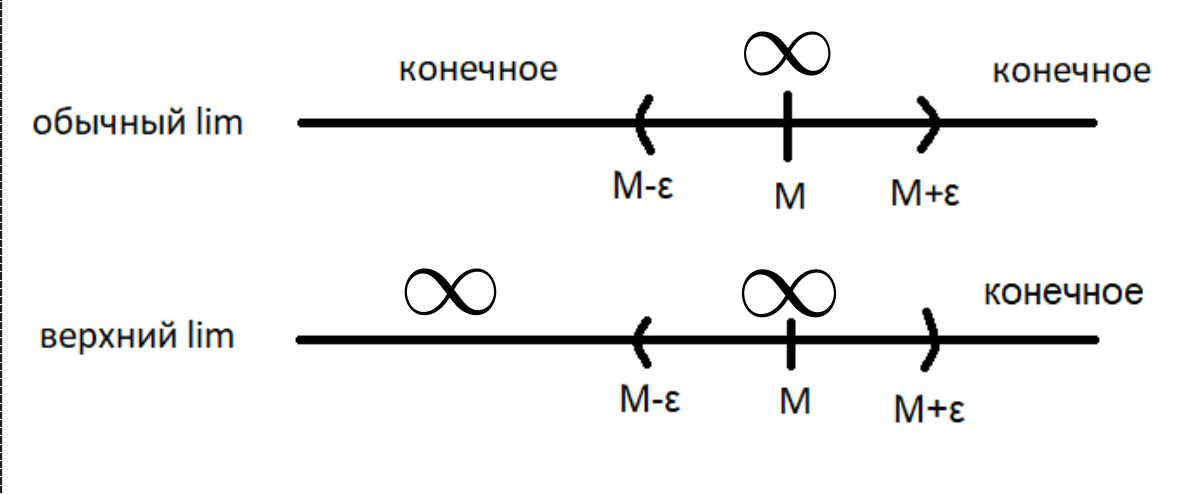
\includegraphics{2.9.1}\\
    Левее $M-\varepsilon$ в случае "обычного" предела находятся конечное число элементов $x_n$, а в случае верхнего предела - $\infty$ число элементов $x_n$.\\
    \textbf{Нижним пределом} последовательности $\{x_n\}$ называется число $m$ (конечное, $\pm \infty$):
    \begin{enumerate}
        \item $\exists$ подпоследовательность $\{x_{n_{k}}\} \Big| \lim_{k\to\infty}x_{n_{k}} = m$.
        \item $\forall$ сходящейся $\{x_{n_{k}}\} \lim_{k\to\infty} x_{n_{k}} \ge m$.\\
        Обозначение: $m = \underline{\lim}_{k\to\infty}x_n$.\\
        Замечание: если $\{x_n\}$ неограниченна сверху, то $\underline{\lim}_{k\to\infty}x_n = -\infty$.\\
        Замечание: если $\{x_n\}$ сходящаяся и $\lim_{n\to\infty} x_n = m$, то $\underline{\lim}_{k\to\infty}x_n = m$.
    \end{enumerate}
    \subsubsection*{Разница между обычным пределом (единственным) и нижним пределом}
    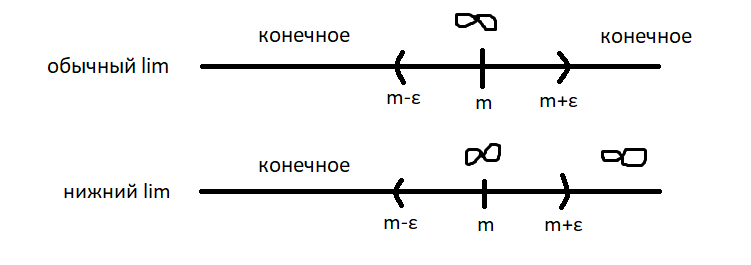
\includegraphics{2.9.2}\\
    Разница между "обычным" пределом и нижним пределом заключается в том, что правее $M+\varepsilon$ в случае "обычного" предела находятся конечное число элементов $x_n$, а в случае нижнего предела - $\infty$ число элементов $x_n$.\\
    Очевидно, $\underline{\lim}_{n\to\infty}x_n \le \overline{\lim}_{n\to\infty}x_n$.
    Для того, чтобы последовательность $\{x_n\}$ имела предел (конечный, $\pm \infty$) $\Leftrightarrow$ чтобы $\underline{\lim}_{n\to\infty} x_n = \overline{\lim}_{n\to\infty} x_n$. В этом случае $\lim_{n\to\infty} x_n = \underline{\lim_{n\to\infty}} x_n = \overline{\lim}_{n\to\infty} x_n$
    
    \subsection{Критерий Коши сходимости числовой последовательности}
    \noindent Последовательность $\{x_n\}$ называется \textbf{фундаментальной}, если она удовлетворяет условию Коши:
    \[ \forall \varepsilon > 0 \text{ } \exists \text{ } n_{0} \text{ } \big| \text{ } \forall n > n_{0}, \forall m > n_{0} \text{ } |x_n - x_{m}| < \varepsilon \]
    \begin{center}
        или
    \end{center}
    \[ \forall \varepsilon > 0 \text{ } \exists \text{ } n_{0} \text{ } \big| \text{ } \forall n > n_{0}, \forall p > 0 \text{ } |x_{n+p} - x_n| < \varepsilon \]
    \subsubsection*{Леммы о фундаментальных последовательностях}
    \noindent \textbf{Лемма 1:} если последовательность $\{x_n\}$ имеет конечный предел, то она фундаментальная.\par\noindent
    \underline{Доказательство:}
    \begin{adjustwidth}{1.5em}{1.5em}
        Пусть $\posl{x}{n}$ - сходящаяся.\\
        Тогда $\exists$ $\lim_{n\to\infty}x_n = a$, т.е.
        \[ \forall \varepsilon > 0 \text{ } \exists \text{ } N = N(\varepsilon) \text{ } \big| \text{ } \forall n > N \implies |x_{n} - a| < \frac{\varepsilon}{2} \]
        Пусть $m > N$ и $n > N$. Рассмотрим $|x_m - x_n|$.
        \[
            |x_m - x_n| = |(x_m - a) - (x_n - a)| \le |x_m - a| + |x_n - a| < \frac{\varepsilon}{2} + \frac{\varepsilon}{2} = \varepsilon
        \]
        Т.е. $\posl{x}{n}$ - фундаментальна.
        \begin{center}
            \textbf{Ч.т.д.}
        \end{center}
    \end{adjustwidth}

    \noindent \textbf{Лемма 2:} если последовательность фундаментальна, то она ограничена.\par\noindent
    \underline{Доказательство:}\par
    \begin{adjustwidth}{1.5em}{1.5em}
        Пусть $\posl{x}{n}$ - фундаментальна. Тогда по условию Коши
        \[ \exists \text{ } n_0 \text{ } \big| \text{ } \forall m,n > n_0 \implies |x_n - x_m| < \varepsilon \]
        Зафиксируем $m = n_0 + 1$. Получим $|x_n - x_{n_0+1}| < \varepsilon$.
        \begin{gather*}
            -\varepsilon < x_n - x_{n_0 + 1} < \varepsilon\\
            x_{n_0 + 1} - \varepsilon < x_n <  x_{n_0 + 1} + \varepsilon
        \end{gather*}
        Обозначим $d = max\{|x_1|, |x_2|, \dots, |x_{n_0}|, |x_{n_0+1} + \varepsilon|\}$.\\
        Тогда
        \[ \forall n \in N \Rightarrow -d \le x_n \le d \]
        То есть $\posl{x}{n}$ ограничена.
        \begin{center}
            \textbf{Ч.т.д.}
        \end{center}
    \end{adjustwidth}

    \noindent \textbf{Лемма 3:} если некоторая подпосл-ть фундаментальной посл-ти сходится, то предел этой подпосл-ти является пределом всей посл-ти.\par\noindent
    \underline{Доказательство:}
    \begin{adjustwidth}{1.5em}{1.5em}
        Пусть $\posl{x}{n}$ - фундаментальная последовательность. Пусть $\posl{x}{n_k}$ - её сходящаяся подпосл-ть.\\
        Пусть $\lim_{k\to\infty}x_{n_k} = a$\\
        Зададим $\varepsilon > 0$\\
        По условию Коши
        \[ \exists \text{ } n_0 \text{ } \big| \text{ } \forall m,n > n_0 \implies |x_n - x_m| < \frac{\varepsilon}{2} \]
        Т.к. $\lim_{k\to\infty}x_{n_k} = a$, т.е.
        \[ \exists \text{ } k_0 = k_0(\varepsilon) \implies |x_{n_k} - a| < \frac{\varepsilon}{2} \]
        Пусть $k_0$ будет таким, чтобы при $k > k_0 \implies n_k > n_0$\\
        \begin{gather*}
            |x_n - a| = |x_n - x_{n_k} + x_{n_k} - a| \le |x_n - x_{n_k}| + |x_{n_k} - a| < \frac{\varepsilon}{2} + \frac{\varepsilon}{2} = \varepsilon \implies \lim_{n\to\infty} x_n = a
        \end{gather*}
        \begin{center}
            \textbf{Ч.т.д.}
        \end{center}
    \end{adjustwidth}

    \subsubsection*{Теорема 2.10.1 (критерий Коши сходимости числовой посл-ти)}\label{th:2.10.1}
    Для того, чтобы посл-ть имела конечный предел $\Leftrightarrow$ чтобы она была фундаментальна.\par\noindent
    \underline{Доказательство:}\par
    \begin{adjustwidth}{1.5em}{1.5em}
        \textbf{Докажем необходимость} ($\Rightarrow$).\\
        Пусть посл-ть имеет конечный предел. Тогда по лемме 1 она фундаментальна.\par\noindent
        \textbf{Докажем достаточность} ($\Leftarrow$).\\
        Пусть посл-ть фундаментальная. Тогда по лемме 2 она ограничена, следовательно по \hyperref[th:2.8.1]{теореме Больцано-Вейерштрасса} можно извлечь сходящуюся подпосл-ть.\\
        Тогда по лемме 3 вся посл-ть будет иметь предел, равный пределу подпосл-ти, т.е. посл-ть сходящаяся.
        \begin{center}
            \textbf{Ч.т.д.}
        \end{center}
    \end{adjustwidth}

    \section{Теория пределов функций. Непрерывность функций в точке и на отрезке.}
    \subsection{Функция. Предел функции в точке.}
    \noindent Пусть $E \subset R$. Пусть $\forall x \in E$ по вполне определённому закону ставится в соответствие единственное число $y$. Тогда говорят, что на множестве $E$ задана \textbf{функция} $y = f(x)$.\par\noindent
    $E$ - область определения функции.\\
    $x$ - независимая переменная (аргумент функции).\\
    $y$ - зависимая переменная (функция).
    \subsubsection*{Определение предела функции в точке по Гейне (в терминах последовательностей)}
    Число $a$ называется пределом функции $f(x)$ в точке $x_0$, если $f(x)$ определена в некоторой окрестности точки $x_0$, быть может за исключением самой точки $x_0$ (такая окрестность называется выколотой окрестностью) и $\forall \posl{x}{n} \text{ } \big| \text{ } \lim_{n\to\infty}x_n = x_0$, порождаемая ею посл-ть $\{f(x_n)\}$ имеет своим пределом точку $a$, т.е. $\lim_{n\to\infty}f(x_n) = a$.\\
    \underline{Запись:}
    \[ \lim_{x \to x_0}f(x) = a \]
    \begin{center}
        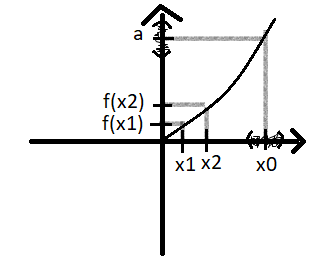
\includegraphics{3.1.1}
    \end{center}
    \underline{Пример:}
    \begin{adjustwidth}{1.5em}{1.5em}
        Рассмотрим такой предел
        \begin{gather*} 
            \lim_{x\to0}\frac{2x^2+x-1}{x-1} =
            \begin{vmatrix}
                \text{Пусть }x_n\text{ - произвольная}\\
                \lim_{n\to\infty}x_n = 0
            \end{vmatrix} =
            \lim_{n\to\infty} \frac{2x_n^2+x_n-1}{x_n-1} =\\
            \frac{\lim_{n\to\infty}(2x_n^2 + x_n - 1)}{\lim_{n\to\infty}(x_n-1)} = \frac{\lim_{n\to\infty}(2x^2_n)+\lim_{n\to\infty}x_n - 1}{\lim_{n\to\infty}x_n - 1} =\\
            \frac{2\lim_{n\to\infty}x_n \times \lim_{n\to\infty}x_n + \lim_{n\to\infty}x_n - 1}{\lim_{n\to\infty}x_n - 1} = \frac{-1}{-1} = 1
        \end{gather*}
        Другой пример: доказать, что $\lim_{x\to0}\sin\frac{1}{x} = \nexists$\par\noindent
        \underline{Доказательство:}
        \begin{adjustwidth}{1.5em}{1.5em}
            Выберем $\posl{x}{n}$ такую, что $\lim_{n\to\infty}x_n = 0$.\\
            \begin{enumerate}
                \item $x_n = \frac{1}{\pi n}$
                \[ \lim_{n\to\infty}\frac{1}{\pi n} \implies \lim_{n\to\infty}\sin \frac{1}{\frac{1}{\pi n}} = \lim_{n\to\infty}\sin \pi n = 0 \]
                \item $x_n = \frac{1}{\frac{\pi}{2} + 2\pi n}$
                \[ \lim_{n\to\infty}\frac{1}{\frac{\pi}{2} + 2\pi n} = 0 \implies \lim_{n\to\infty}\sin \frac{1}{\frac{1}{\frac{\pi}{2} + 2\pi n}} = \lim_{n\to\infty} \sin(\frac{\pi}{2} + 2\pi n) = \lim_{n\to\infty}\sin \frac{\pi}{2} = 1 \]
                Поэтому $\lim_{x\to 0}\sin \frac{1}{x} = \nexists$.
                \begin{center}
                    \textbf{Ч.т.д.}
                \end{center}
            \end{enumerate}
        \end{adjustwidth}
    \end{adjustwidth}
    
    \subsubsection*{Определение предела функции в точке по Коши}
    Число $a$ называется пределом функции $f(x)$ в точке $x_0$, если $f(x)$ определена в окрестности точки $x_0$, быть может за исключением самой точки $x_0$ и, если $\forall \varepsilon > 0$ $\exists$ $\delta = \delta(\varepsilon)$ $\big|$ $|x - x_0| < \delta \implies |f(x) - a| < \varepsilon$\\
    \begin{center}
        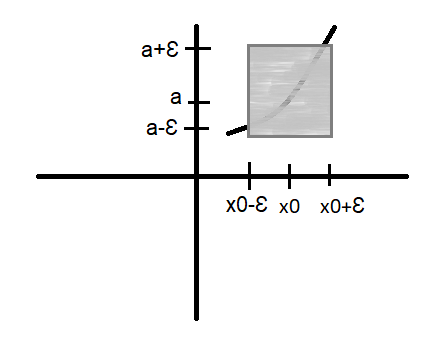
\includegraphics{3.1.2}
    \end{center}
    Если $x$ находятся в $\delta$-окрестности точки $x_0$, то все значения $f(x)$ располагаются в полосе шириной $2\varepsilon$.
    \subsubsection*{Теорема 3.1.1}\label{th:3.1.1}
    Определения предела функции $f(x)$ в точке $x_0$ по Гейне и по Коши эквивалентны.\par\noindent
    \underline{Доказательство:}
    \begin{adjustwidth}{1.5em}{1.5em}
        \begin{enumerate}
            \item \textbf{Докажем Гейне $\rightarrow$ Коши}\\
            Пусть функция имеет предел в точке $x_0$ в смысле Гейне.\\
            Предположим противное. Пусть функция $f(x)$ не имеет предел в точке $x_0$ в смысле Коши. Это значит, что $\exists$ хотя бы одно $\varepsilon_0$, для которого нельзя подобрать нужное $\delta$.\\
            То есть $\forall \delta$ среди $x$, удовлетворяющих неравенству $|x-x_0| < \delta$ должно найтись хотя бы одно $x = x(\delta) : |f(x(\delta)) - a| \ge \varepsilon$\\
            Составим последовательность. Выберем $\delta = \frac{1}{k}$ и для каждого $k$ будем искать точку $x_k$ для которой не выполняется определение Коши.
            \begin{enumerate}
                \item $k = 1$ $\delta = 1$ $|x_1 - x_0| < 1 \implies |f(x_1) - a| \ge \varepsilon_0$\\
                такой $x_1$ $\exists$
                \item $k = 2$ $\delta = \frac{1}{2}$ $|x_2 - x_0| < \frac{1}{2} \implies |f(x_2) - a| \ge \varepsilon_0$\\
                такой $x_2$ $\exists$
                \item $k = 3$ $\delta = \frac{1}{3}$ $|x_3 - x_0| < \frac{1}{3} \implies |f(x_3) - a| \ge \varepsilon_0$\\
                такой $x_3$ $\exists$
            \end{enumerate}
            То есть $\forall k > 0$ $|x_k - x_0| < \frac{1}{k} \implies \lim_{k\to\infty} x_k = x_0$, но тогда $|f(x_k) - a| \ge \varepsilon_0$, то есть $\lim_{k\to\infty} f(x_k) \ne a$. Получили противоречие, т.к. по Гейне $\lim_{k\to\infty} f(x_k) = a$.
            \item \textbf{Докажем Коши $\rightarrow$ Гейне}\\
            Пусть функция имеет предел по Коши.\\
            Зададим произвольную последовательность $\posl{x}{n} : \lim_{n\to\infty} x_n = x_0$.\\
            Так как определение по Коши выполняется, то
            \[
                \forall \varepsilon > 0 \text{ } \exists \text{ } \delta = \delta(\varepsilon) : |x - x_0| < \delta \implies |f(x) - a| < \varepsilon
            \]
            \begin{gather*}
                \text{Т.к. } \lim_{n\to\infty}x_n = x_0 \implies \forall \varepsilon > 0 \text{ } \exists n_0 = n_0(\varepsilon) : |x_n - x_0| < \delta \implies\\
                |f(x_n) - a| < \varepsilon \implies \lim_{x\to x_0} f(x) = a
            \end{gather*}
        \end{enumerate}
        \begin{center}
            \textbf{Ч.т.д.}
        \end{center}
    \end{adjustwidth}
    \subsubsection*{Предел функции в бесконечно удалённой точки}
    \[\lim_{x\to +\infty}f(x) = a\]
    Число $a$ называется пределом функции $f(x)$ при $x \to +\infty$, если 
    \[ \forall \varepsilon > 0 \text{ } \exists \text{ } k = k(\varepsilon) : x > k \implies |f(x) - a| < \varepsilon \]
    \underline{Упр.:} уметь расписывать \textbf{ВСЕГДА и ВЕЗДЕ}
    \begin{adjustwidth}{1.5em}{1.5em}
        \begin{gather*}
            \lim_{x\to -\infty}f(x) = a;
            \lim_{x\to x_0}f(x) = \infty;
            \lim_{x\to x_0}f(x) = -\infty;\\
            \lim_{x\to +\infty}f(x) = +\infty;
            \lim_{x\to +\infty}f(x) = -\infty;
            \lim_{x\to -\infty}f(x) = +\infty;\\
            \lim_{x\to -\infty}f(x) = -\infty
        \end{gather*}
        Например, распишем последнее.
        Нужны два параметра. В определении Коши есть $\delta$ для $x$ (аргумента) и $\varepsilon$ для $y$ (функции).\\
        Т.к. $x \to -\infty$, то мы не можем использовать $\delta$ (она используется для малых величин), поэтому введём параметр $K$ вместо $\delta$.\\
        Т.к. $\lim_{x\to -infty}f(x) = -\infty$, то мы не можем использовать $\varepsilon$ (он используется для малых величин), поэтому введём параметр $M$ вместо $\varepsilon$.\\
        Тогда определение принимает вид:
        \[
            \forall M > 0 \text{ } \exists \text{ } K = K(M) > 0 : x < -K \implies f(x) < -M
        \]
    \end{adjustwidth}

    \subsection{Односторонние пределы}
    Если значение функции $f(x)$ стремится к числу $a$ по мере стремления $x$ к $x_0$ со стороны меньших (больших) значений, то число $a$ называют пределом функции $f(x)$ в точке $x_0$ слева (справа)
    \begin{center}
        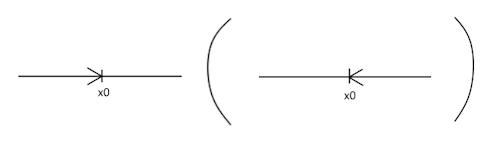
\includegraphics{3.2.1}
    \end{center}
    Обозначение:
    \begin{itemize}
        \item предел слева: $\lim_{x\to x_0 - 0}f(x) = f(x_0 - 0) = a$
        \item предел справа $\lim_{x\to x_0 + 0}f(x) = f(x_0 + 0) = a$
    \end{itemize}
    \underline{Пример:}
    \begin{adjustwidth}{1.5em}{1.5em}
        \[
            \lim_{x\to 0-0} 2^{\frac{1}{x}} = 0; \lim_{x\to 0+0} 2^{\frac{1}{x}} = \infty
        \]
        \begin{center}
            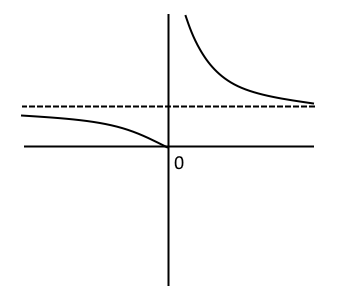
\includegraphics{3.2.2}
        \end{center}
    \end{adjustwidth}
    \underline{Пример 2:}
    \begin{adjustwidth}{1.5em}{1.5em}
        \[f(x) = \text{sign } x = \begin{cases}
            1, x > 0\\
            0, x = 0\\
            -1, x < 0
        \end{cases}
        \]
        \begin{center}
            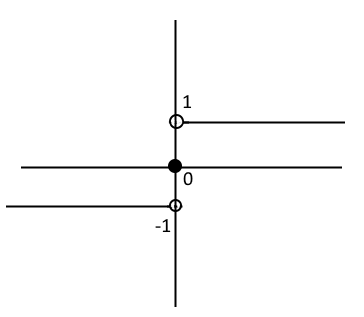
\includegraphics{3.2.3}
        \end{center}
        \[
            \lim_{x\to 0-0} \text{sign } x = -1; \lim_{x\to 0+0} \text{sign } x = 1
        \]
    \end{adjustwidth}
    \underline{Утверждение:} для того, чтобы существовал обычный двусторонний предел функции в точке $x_0$ $\Leftrightarrow$ чтобы в этой точке существовали левый и правый односторонние пределы и чтобы они были равны.
    \[ \lim_{x \to x_0} f(x) = a \Leftrightarrow \lim_{x \to x_0 - 0}f(x) = \lim_{x \to x_0 + 0} f(x) \]

    \subsection{Свойства пределов функций}
    \subsubsection*{Теорема 3.3.1}\label{th:3.3.1}
    Если $\lim_{x\to x_0}f(x) = a$, где $a$ - конечное число, то в некоторой окрестности точки $x_0$ $f(x)$ ограничена.\par\noindent
    \underline{Доказательство:}
    \begin{adjustwidth}{1.5em}{1.5em}
        По определению Коши предела функции в точке:
        \[ \forall \varepsilon > 0 \text{ } \exists \text{ } \delta = \delta(\varepsilon) : |x - x_0| < \delta \implies |f(x) - a| < \varepsilon \]
        \[ -\varepsilon < f(x) - a < \varepsilon \]
        \[ a - \varepsilon < f(x) < a + \varepsilon \]
        \begin{center}
            \textbf{Ч.т.д.}
        \end{center}
    \end{adjustwidth}

    \subsubsection*{Теорема 3.3.2 (о сохранении знака)}\label{th:3.3.2}
    Если функция $f(x)$ имеет в точке $x_0$ не равный нулю конечный предел $a$, то $\exists$ окрестность точки $x_0 : \forall x$, принадлежащего этой окрестности, выполняется
    \begin{gather*}
        f(x) > \frac{a}{2}, a > 0\\
        f(x) < \frac{a}{2}, a < 0
    \end{gather*}
    \underline{Доказательство:}
    \begin{adjustwidth}{1.5em}{1.5em}
        $\lim_{x\to x_0}f(x) = a$\\
        Обозначим $U(x_0)$ - окрестность точки $x_0$\\
        Тогда $\forall x \in U(x_0) : |f(x) - a| < \varepsilon = \frac{|a|}{2}$
        \[a - \frac{|a|}{2} < f(x) < a + \frac{|a|}{2}\]
        \begin{align*}
            a &> 0 & a &< 0\\
            f(x) &> a - \frac{a}{2} & f(x) &< a - \frac{a}{2}\\
            f(x) &> \frac{a}{2} & f(x) &< -\frac{|a|}{2}
        \end{align*}
        \begin{center}
            \textbf{Ч.т.д.}
        \end{center}
    \end{adjustwidth}

    \subsubsection*{Теорема 3.3.3}\label{th:3.3.3}
    Если $f(x) = c$ (константа), то $\lim_{x\to x_0}f(x) = c$ - уже доказана.
    
    \subsubsection*{Теорема 3.3.4}\label{th:3.3.4}
    Если $\lim_{x\to x_0}f(x) = a, \lim_{x \to x_0}g(x) = b$ и $\forall x \in R$ из окрестности точки $x_0$:
    \[ f(x) \le g(x) \implies a \le b \]
    
    \subsection{Непрерывность функции в точке. Разрывы I и II родов.}
    \noindent Функция $f(x)$ называется непрерывной в точке $x_0$, если 
    \[\lim_{x\to\infty}f(x) = f(x_0)\]
    \[\lim_{x\to\infty}f(x) = f(\lim_{x\to\infty}x) = f(x_0)\]
    \noindent Т.е. для непрерывности в точке функции множества меняются знаками предела и функции
    \begin{enumerate}
        \item Через прирождение\\
        $\varDelta x = x - x_0$ - прирождение аргумента\\
        $\varDelta y = y - y_0$ - прирождение функции\\
        Функция $f(x)$, направленная в точке $x_0$, если $\lim_{\delta x = 0} \delta y = 0$
        \item Определение Гейне\\
        Функция $f(x)$ называется непрерывной в точке $x_0$, если для $\forall$ последовательности $\lim_{x\to\infty} x_n = x_0$\\
        Порождающая её последовательность $f(x_n)$ $\lim_{n\to\infty} f(x_0) = f(x_0)$
        \item Определение Коши\\
        Функция $f(x)$ называется непрерывной в точке $x_0$ $\forall \varepsilon > 0$ $\exists$ $(\delta - \delta \varepsilon)$
    \end{enumerate}
    Функция $f(x)$ имеет в точке $x_0$ разрыв II рода, если хотя бы один из пределов (справа или слева) не существует или бесконечен.\par\noindent
    \underline{Пример 1:} рассмотрим при $x \ne 2$
    \begin{gather*}
        f(x) = \frac{x^2 - 4}{x-2}\\
        f(x) = \frac{x^2-4}{x-2} = x+2\\
        f(2) = \nexists\\
        \lim_{x\to 2-0} f(x) = \lim_{x\to 2-0}(x+2) = 4\\
        \lim_{x\to 2+0} f(x) = 4
    \end{gather*}
    \begin{center}
        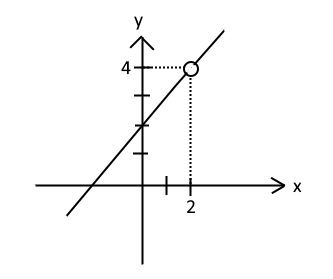
\includegraphics{3.4.2}
    \end{center}
    $f(x)$ непрерывна $\forall x \in R$, кроме $x=2$, где $f(x)$ терпит разрыв I рода устранений.\par\noindent
    \underline{Замечание:} рассмотрим 
    $ g(x) = \begin{cases}
        f(x), x \ne 2\\
        4, x = 2
    \end{cases}$;
    \noindent $g(x)$ непрерывна $\forall x \in R$\par\noindent
    \underline{Пример 2:} рассмотрим
    \[
        f(x) = [x] \text{ - целая часть }x, x > 0
    \]
    \begin{center}
        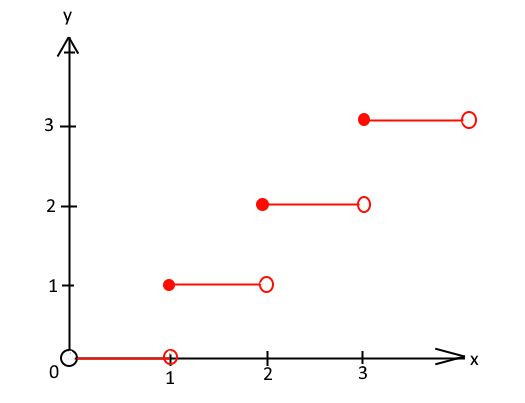
\includegraphics{3.4.3}
    \end{center}
    \begin{gather*}
        f(x) = 1\\
        \lim_{x\to 1-0} [x] = 0\\
        \lim_{x \to 1+0} [x] = 1
    \end{gather*}
    $\forall x \in N$ $f(x)$ терпит разрыв I рода (скачок), в остальных $x > 0$ $f(x)$ - непрерывна.\par\noindent
    \underline{Пример 3:} рассмотрим
    \[ f(x) = \frac{1}{x} \]
    \begin{center}
        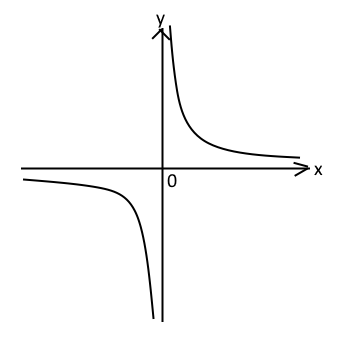
\includegraphics{3.4.4}
    \end{center}
    \begin{gather*}
        f(0) = \nexists\\
        \lim_{x \to 0-0} \frac{1}{x} = -\infty\\
        \lim_{x \to 0+0} \frac{1}{x} = \infty
    \end{gather*}
    $f(x)$ непрерывна $\forall x \in R$, кроме $x = 0$, где она терпит разрыв II рода.\\

    \subsection{Замечательные пределы}
    \subsubsection*{Теорема 3.5.1 (I Замечательный предел)}\label{th:3.5.1}
    \[ \lim_{x\to 0}\frac{\sin x}{x} = \lim_{x\to 0} \frac{x}{\sin x} = 1 \]\noindent
    \underline{Доказательство:}
    \begin{adjustwidth}{1.5em}{1.5em}
        \begin{center}
            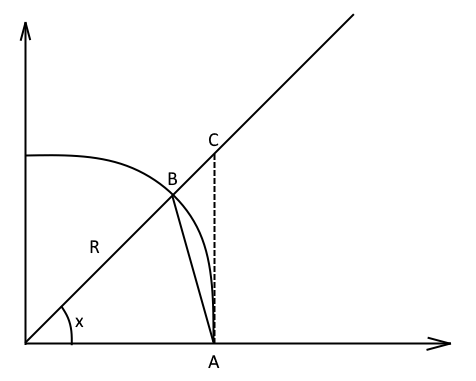
\includegraphics{3.5.1}
        \end{center}
        Рассмотрим в координатной плоскости круг радиуса $R$ с центром в начале координат\\
        \begin{gather*} 
            S_{\triangle OAB} < S_{\text{сект}OAB} < S_{\triangle OAC}\\
            \frac{1}{2}R^2\sin x < \frac{1}{2}R^2 x < \frac{1}{2} R^2 \tg  x\\
            \sin x < x < \tg  x \text{ } \big| : \sin x \text{ } (\text{пусть } \sin x > 0)\\
            1 < \frac{x}{\sin x} < \frac{1}{\cos x}\\
            \lim_{x\to 0} 1 = 1, \lim_{x\to 0} \frac{1}{\cos x} = 1 \implies \lim_{x\to 0} \frac{1}{\sin x} = 1
        \end{gather*}
        \begin{center}
            \underline{Замечание:} $f(x) = \cos x$ и $\frac{x}{\sin x}$, поэтому неравенство будет выполняться для $\frac{-\pi}{2} < x < 0$
        \end{center}
    \end{adjustwidth}

    \subsubsection*{Теорема 3.5.2 (II Замечательный предел)}\label{th:3.5.2}
    \[ \lim_{x\to\infty}(1 + \frac{1}{x})^x = e \]
    \[ \lim_{x\to 0}(1 + x)^{\frac{1}{x}} = e \]\noindent
    \underline{Доказательство:}
    \begin{adjustwidth}{1.5em}{1.5em}
        Надо показать, что \[\lim_{x\to 0-0} (1 + x)^{\frac{1}{x}} = \lim_{x\to 0+0}(1+x)^{\frac{1}{x}} = e\]
        Замена: \[x = \frac{1}{y} \implies \lim_{y\to -\infty}(1 + \frac{1}{y})^y = \lim_{y\to\infty}(1 + \frac{1}{y})^y = e\]
        \underline{Замечание:} будем считать известным фактом, что $\forall n \in N$ верно $\lim_{n\to\infty}(1+\frac{1}{n})^n = e$.\par\noindent
        Пусть $x_n \to \infty$ (доказываем по определению Гейне)\\
        Покажем, что $\lim_{x_n\to\infty}(1 + \frac{1}{x_n})^{x_n} = e$. $\posl{x}{n}$ - произвольная посл-ть: $\lim_{n\to\infty}x_n = \infty$\\
        Рассмотрим посл-ть $k_n = [x_n]$ - целая часть $x_n$.\\
        \begin{gather*}
            k_n \le x_n < k_n + 1\\
            \frac{1}{k_n + 1} < \frac{1}{x_n} \le \frac{1}{k_n}\\
            1 + \frac{1}{k_n + 1} < 1 + \frac{1}{x_n} \le 1 + \frac{1}{k_n}\\
            (1 + \frac{1}{k_n + 1})^{k_n} < (1 + \frac{1}{x_n})^{k_n} \le (1 + \frac{1}{k_n})^{k_n}\\
            \text{т.к. } k_n \le x_n < k_n + 1\\
            (1 + \frac{1}{k_n + 1})^{k_n} < (1 + \frac{1}{x_n})^{k_n} \le (1 + \frac{1}{k_n})^{k_n+1}\\
        \end{gather*}
        \begin{enumerate}
            \item \[\lim_{n\to\infty}(1+\frac{1}{k_n+1})^{k_n+1-1} = \lim_{n\to\infty}(1+\frac{1}{k_n+1})^{k_n+1}(1+\frac{1}{k_n+1})^{-1} = e \times 1 = e\]
            \item \[\lim_{n\to\infty}(1+\frac{1}{k_n})^{k_n+1} = \lim_{n\to\infty}(1+\frac{1}{k_n})^{k_n}(1+\frac{1}{k_n})^{1} = e \times 1 = e\]
        \end{enumerate}
        Тогда $\lim_{x_n \to \infty}(1 + \frac{1}{x_n})^{x_n} = e$ (по \hyperref[th:2.2.5]{теореме о двух милиционерах})
        Рассмотрим $x_n \to -\infty$. Замена: $x_n' = -x_n$.\\
        Рассмотрим $\lim_{x_n \to -\infty}(1+\frac{1}{x_n})^{x_n} = \lim_{x_n'\to\infty}(1 + \frac{1}{-x_n'})^{-x_n'} = e$\\
        \begin{center}
            \textbf{Ч.т.д.}
        \end{center}
    \end{adjustwidth}

    \subsection{Эквивалентные бесконечно малые функции в точке}
    \noindent Функция $f(x)$ называется беск. малой при $x \to x_0$, если $\lim_{x \to x_0}f(x) = 0$\\
    \underline{Замечание:} Функция, которая является беск. м. в одной точке, может не быть беск. б. в другой точке.\par\noindent
    \subsubsection*{Теорема 3.6.1}\label{th:3.6.1}
    Сумма и произведения конечного числа беск. м. функция в точке есть функция беск. м. в точке.
    \subsubsection*{Теорема 3.6.2}\label{th:3.6.2}
    Произведение беск. м. функции в точке на ограниченную есть беск. м. функция в точке.\par\noindent
    \underline{Доказательство:}
    \begin{adjustwidth}{1.5em}{1.5em}
        Пусть $f(x)$ - беск. м. функция в точке $x_0 \implies \lim_{x\to x_0}f(x)=0$\\
        Пусть $g(x)$ - ограничена в окрестности точки $x_0$ ($u(x_0)$) $\implies \exists$ $M : |g(x)| \le M$\\
        $0 \le |f(x)g(x)| \le M|f(x)|$\\
        По \hyperref[th:2.2.5]{теореме о двух милиционерах} так как $\lim_{x\to x_0}0 = 0$ и $\lim_{x\to x_0}M|f(x)| = M \times 0 = 0$, то $\lim_{x\to x_0}|f(x)g(x)| = 0 \implies \lim_{x\to x_0}f(x)g(x) = 0$
        \begin{center}
            \textbf{Ч.т.д.}
        \end{center}
    \end{adjustwidth}
    \underline{Пример:}
    \begin{adjustwidth}{1.5em}{1.5em}
        \[\lim_{x\to0} x\sin \frac{1}{x} = 0\]
        $x$ - беск. м.\\
        $\sin \frac{1}{x}$ - огр.
    \end{adjustwidth}
    \subsubsection*{Эквивалентность беск. м. функций}
    \noindent Пусть $f(x)$ и $g(x)$ являются беск. м. функциями в точке $x_0$. Тогда они называются эквивалентными беск. м. функциями в точке $x_0$, если
    \[ \lim_{x\to x_0}\frac{f(x)}{g(x)} = 1 \]
    Обозначение: $f(x) \sim g(x), x \to x_0$\\
    Например, $\sin x \sim x, x \to 0$
    \begin{center}
        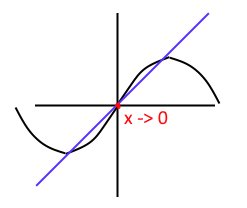
\includegraphics{3.6.1}
    \end{center}
    \underline{Замечание:} если $f_1(x) \sim f_2(x), x \to x_0$, а $g_1(x) \sim g_2(x), x \to x_0$, то
    \[ \lim_{x\to x_0}\frac{f_1(x)}{g_1(x)} = \lim_{x\to x_0}\frac{f_2(x)}{g_2(x)} = \lim_{x\to x_0}\frac{f_2(x)}{g_1(x)} = \lim_{x\to x_0}\frac{f_1(x)}{g_2(x)} \]
    \begin{adjustwidth}{1.5em}{1.5em}
        При нахождении предела дроби можно заменять на эквивалентные беск. м. или числитель, или знаменатель, или и то, и другое (но не часть числителя или знаменателя).
        \begin{center}
            Так \textbf{НЕЛЬЗЯ}:
        \end{center}
        \[ \tg  x - \sin x \sim^? 0 \]
    \end{adjustwidth}
    Основные эквивалентности при $x \to 0$
    \begin{enumerate}
        \item $\sin x \sim x$
        \item $\tg x \sim x$
        \item $\ln(1+x) \sim x$
        \item $e^x - 1 \sim x$
        \item $a^x - 1 \sim x \ln a$
        \item $(1+x)^m - 1 \sim mx$
        \item $\arcsin x \sim x$
        \item $\arctg x \sim x$
        \item $1 - \cos x \sim \frac{x^2}{2}$
    \end{enumerate}
    \underline{Доказательство:}
    \begin{adjustwidth}{1.5em}{1.5em}
        \begin{enumerate}
            \item доказано (I Замечательный предел)
            \item \[\lim_{x\to 0}\frac{\tg  x}{x} = \lim_{x\to 0}\frac{\sin x}{x \cos x} = 1\]
            \item \[\lim_{x\to 0}\frac{\ln(1+x)}{x} = \lim_{x\to 0}\frac{1}{x} \times \ln(1+x) = \lim_{x\to 0}\ln(1+x)^{\frac{1}{x}} = \ln \lim_{x\to 0}(1+x)^{\frac{1}{x}} = \ln e = 1\]
            \item частный случай пункта 5 $(a = e)$
            \item \[\lim_{x\to 0}\frac{a^x-1}{x \ln a} = \begin{vmatrix}
                a^x - 1 = y\\
                x \to 0 \implies y \to 0\\
                \ln a^x = \ln(1+y)\\
                x\ln a = \ln(1+y)
            \end{vmatrix} = \lim_{y\to 0}\frac{y}{\ln(1+y)} = 1\]
            \item \begin{gather*}
                \lim_{x\to 0}\frac{(1+x)^m-1}{mx} = \lim_{x\to 0}\frac{(1+x)^m-1}{\ln(1+x)}\frac{\ln(1+x)}{mx} =\\= \lim_{x\to 0}\frac{(1+x)^m-1}{\ln (1+x)} \lim_{x\to 0}\frac{\ln(1+x)}{mx} = \lim_{x\to 0}\frac{(1+x)^m-1}{m\ln(1+x)} = \begin{vmatrix}
                    (1+x)^m - 1 = y\\
                    x \to 0 \implies y \to 0\\
                    (1+x)^m = y + 1\\
                    \ln(1+x)^m = \ln(1+y)\\
                    m\ln(1+x) = \ln(1+y)
                \end{vmatrix} =\\= \lim_{y\to 0}\frac{y}{\ln(1+y)} = 1
            \end{gather*}
            \item \[\lim_{x\to 0}\frac{\arcsin x}{x} = \begin{vmatrix}
                \arcsin x = y\\
                x \to 0 \implies y \to 0\\
                x = \sin y
            \end{vmatrix} = \lim_{y\to 0}\frac{y}{\sin y} = 1\]
            \item \[\lim_{x\to 0}\frac{\arctg x}{x} = \begin{vmatrix}
                \arctg x = y\\
                x \to 0 \implies y \to 0\\
                x = \tg  y
            \end{vmatrix} = \lim_{y\to 0}\frac{y}{\tg  y} = \lim_{y\to 0}\frac{y\cos y}{\sin y} = 1\]
            \item \[\lim_{x\to 0}\frac{1-cos x}{\frac{x^2}{2}} = \lim_{x\to 0}\frac{2\sin^2(\frac{x}{2})}{\frac{x^2}{2}} = 1\]
        \end{enumerate}
    \end{adjustwidth}

    \subsection{Порядок переменной. Сравнение функций в окрестности заданной точки.}
    \noindent Рассмотрим функции $f(x)$ и $g(x)$, заданные в $u(x_0)$ за исключением быть может самой точки $x_0$.\par\noindent
    $x_0$ - конечная, $\pm \infty$.\\
    Пусть $g(x) \ne 0$ $\forall x \in u(x_0)$.\par\noindent
    Если $\lim_{x\to x_0}\frac{f(x)}{g(x)} = \left[ \frac{0}{0} \right] = 0$, то в этом случае $f(x) = o(g(x))$, ($o$ читается как "$o$ малое"), т.е. $f(x)$ является беск. м. более высокого порядка малости, чем $g(x)$ при $x \to x_0$.\par\noindent
    Если $\lim_{x\to x_0}\frac{f(x)}{g(x)} = k \ne 0$, то $f(x)$ и $g(x)$ называются беск. малой одного порядка при $x \to x_0$.\par\noindent
    Беск. малая $f(x)$ при $x \to x_0$ имеет $k$-ый порядок малости по отношению к $g(x)$ при $x \to x_0$, если $f(x)$ имеет тот же порядок малости, что и $g^k(x)$, т.е. $\lim_{x\to x_0}\frac{f(x)}{g^k(x)} = 0$
    
    \subsubsection*{Теорема 3.7.1}\label{th:3.7.1}
    Для того, чтобы функции $f(x)$ и $g(x)$ были эквивалентными при $x \to x_0 \Leftrightarrow f(x) = g(x) + o(g(x)), x \to x_0$\par\noindent
    \underline{Доказательство:}
    \begin{adjustwidth}{1.5em}{1.5em}
        \textbf{Докажем необходимость ($\Rightarrow$)}\par\noindent
        Пусть $f(x) \sim g(x), x \to x_0$. Тогда по определению $\lim_{x \to x_0}\frac{f(x)}{g(x)} = 1$.\\
        Следовательно, \begin{gather*}
            \lim_{x\to x_0}\varepsilon(x) = 0\\
            \frac{f(x)}{g(x)} = 1 + \varepsilon(x) \Big| \times g(x)\\
            f(x) = g(x) + \varepsilon(x) g(x) = g(x) + o(g(x))
        \end{gather*}\noindent
        \textbf{Докажем достаточность ($\Leftarrow$)}\par\noindent
        Пусть $f(x) = g(x) + o(g(x)), x \to x_0$\\
        Например, 
        \begin{gather*}
            f(x) = g(x) + \varepsilon(x) g(x) \Big| : g(x)\\
            \frac{f(x)}{g(x)} = 1 + \varepsilon(x)\\
            \lim_{x \to x_0} \frac{f(x)}{g(x)} = 1
        \end{gather*}
        Т.е. $f(x) \sim g(x), x \to x_0$.
        \begin{center}
            \textbf{Ч.т.д.}
        \end{center}
    \end{adjustwidth}

    Функция $f(x)$ называется функцией, ограниченной относительно функции $g(x)$ в $u(x_0)$, если ограничена функция $\frac{f(x)}{g(x)}$, т.е.
    \[ \left|\frac{f(x)}{g(x)}\right| \le c \text{ или } \left|f(x)\right| \le c\left|g(x)\right| \]
    В этом случае $f(x) = O(g(x)), x \to x_0$\\
    $f(x) = O(1), x \to x_0$ = "функция $f(x)$ ограничена.
    
    \subsection{Глобальные свойства функций, непрерывных на отрезке}
    \noindent Функция $f(x)$ называется непрерывной на отрезке $[a; b]$, если она непрерывна в каждой точке интервала $(a; b)$, в точке $x = a$ справа, в точке $x = b$ слева.
    \subsubsection*{Теорема 3.8.1 (I-ая теорема Вейерштрасса)}\label{th:3.8.1}
    Если функция $f(x)$ непрерывна на $[a; b]$, то она ограничена на нём, т.е.
    \[ \exists M > 0 : \left|f(x)\right| \le M \text{ } \forall x \in [a; b] \]\noindent
    \underline{Доказательство:}
    \begin{adjustwidth}{1.5em}{1.5em}
        Предположим противное. Пусть $f(x)$ непрерывна на $[a; b]$, но при этом не ограничена на нём.\\
        Составим последовательность $x_n$ следующим образом:
            \begin{gather*}
                \exists x_1 \in [a; b] : f(x_1) > 1\\
                \exists x_2 \in [a; b] : f(x_2) > 2\\
                \vdots\\
                \exists x_n \in [a; b] : f(x_n) > 2\\
                \vdots
            \end{gather*}
        В результате получили посл-ть $\posl{x}{n}$. Она ограничена ($\forall n$ $x_n \in [a; b]$). По \hyperref[th:2.8.1]{теореме Больцано-Вейерштрасса} из неё можно извлечь сходяющуся подпосл-ть $x_{n_k}$\\
        Пусть $\lim_{k\to\infty}x_{n_k} = \alpha$\\
        Так как $f(x)$ непрерывна на $[a; b]$, то по определению $\lim_{x\to x_0} f(x) = f(x_0)$\\
        В нашем случае $\lim_{k\to\infty} f(x_{n_k}) = f(\lim_{k\to\infty}x_{n_{k}}) = f(\alpha)$ - конечное число (в силу непрерывности)\\
        Однако $f(\alpha)$ является беск. б. по построению $x_n$ ($f(x_n)$ беск. б.), $f(\alpha) = \infty$.\\
        Получили противоречие, т.е. $f(x)$ ограничена.
        \begin{center}
            \textbf{Ч.т.д.}
        \end{center} 
    \end{adjustwidth}
    \subsubsection*{Теорема 3.8.2 (II-ая теорема Вейерштрасса)}\label{th:3.8.2}
    Среди значений, которые на отрезке $[a; b]$ принимает непрерывная функция, существует наибольшее и наименьшее значения (в том числе может быть и в крайних точках).\par\noindent
    \underline{Доказательство:}
    \begin{adjustwidth}{1.5em}{1.5em}
        По \hyperref[th:3.8.1]{I-ой теореме Вейерштрасса} $f(x)$ ограничена сверху, т.е. $\exists k : f(x) \le k \text{ }  \forall x \in [a; b]$\\
        Тогда существует точная верхняя грань $f(x)$ на $[a; b]$. $M = \sup f(x), x \in [a; b]$\\
        Составим вспомогательную посл-ть $\posl{x}{n}$ на основе свойства $\sup f(x)$.
        \begin{gather*}
            \exists x_1 : M - 1 < f(x_1) \le M\\
            \exists x_2 : M - \frac{1}{2} < f(x_2) \le M\\
            \vdots\\
            \exists x_n : M - \frac{1}{n} < f(x_n) \le M\\
            \vdots
        \end{gather*}
        $\posl{x}{n}$ ограничена ($\forall n x_n \in [a; b]$)\\
        Тогда по \hyperref[th:2.8.1]{теореме Больцано-Вейерштрасса} из неё можно извлечь сходящуюся подпосл-ть $x_{n_k}, \lim_{k\to\infty}x_{n_k} = \alpha$
        \begin{enumerate}
            \item С одной стороны, $f(x)$ непрерывна на $[a; b] \implies \lim_{k\to\infty}f(x_{n_k}) = f(\lim_{k\to\infty}x_{n_k}) = f(\alpha)$
            \item С другой стороны $M - \frac{1}{n} < f(x_n) \le M$, следовательно
            \[
                M - \frac{1}{n_k} < f(x_{n_k}) \le M
            \]
            Т.к. $\lim_{k\to\infty} (M - \frac{1}{n_k}) = M$ и $\lim_{k\to\infty} M = M$, то $\lim_{k\to\infty}f(x_{n_k}) = M$ (по т. о двух милиционерах), т.е. $f(\alpha) = M$.\\
            $\beta \in [a; b] : f(\beta) = m$
        \end{enumerate}
    \end{adjustwidth}
    \subsubsection*{Теорема 3.8.3 (Теорема Больцано-Коши)}\label{th:3.8.3}
    Если функция $f(x)$ непрерывна на $[a; b]$ и $f(a) = m, f(b) = n$, то на интервале $(a; b)$ $f(x)$ по крайней мере один раз принимает значение $p$, заключённое между $m$ и $n$.
    \begin{center}
        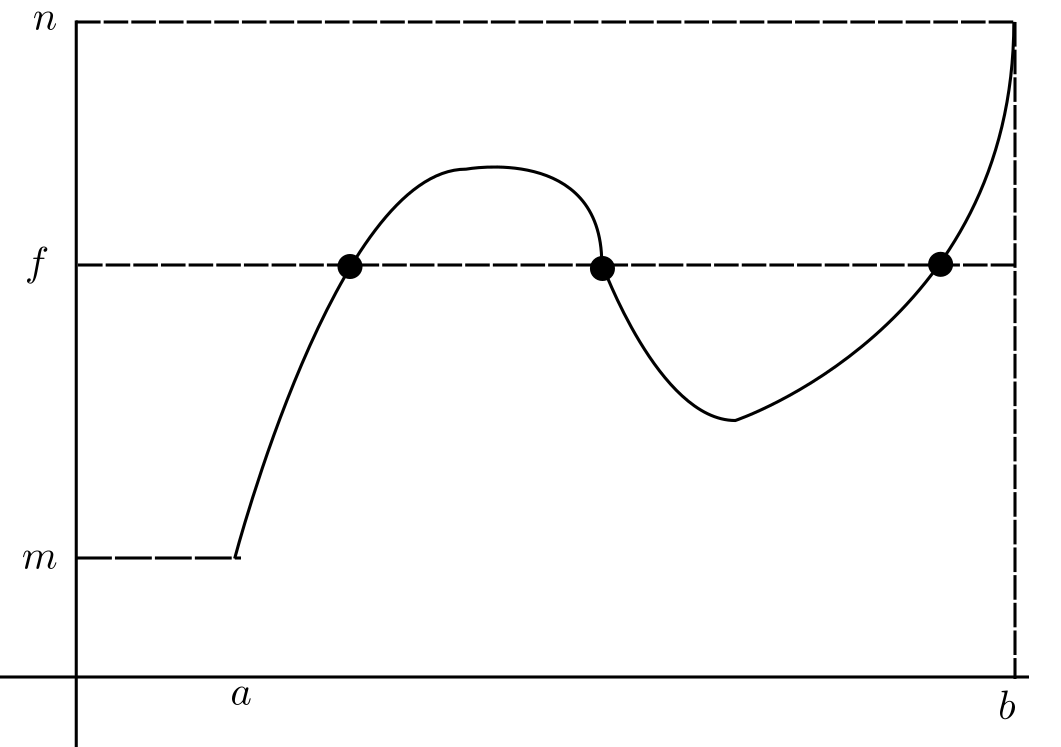
\includegraphics{3.8.1}
    \end{center}
    \underline{Доказательство:}
    \begin{adjustwidth}{1.5em}{1.5em}
        Для доказательства надо найти точку $\xi$, $f(\xi) = p$.\\
        Разобъём отрезок $[a; b]$ на 2 равных отрезка точкой $\frac{a + b}{2}$\\
        Варианты:
        \begin{enumerate}
            \item $f(\frac{a+b}{2}) = p \implies \xi = \frac{a+b}{2}$. \textbf{Ч.т.д.}
            \item $f(\frac{a+b}{2}) \ne p$. Тогда либо $f(\frac{a+b}{2}) < p$, либо $f(\frac{a+b}{2}) > p$.\\
            В первом случае далее выберем отрезок $[\frac{a+b}{2}; b]$, во втором - $[a; \frac{a+b}{2}]$. Переобозначим выбранный отрезок $[a_1; b_1]$, $f(a_1) < p < f(b_1)$. $b_1 - a_1 = \frac{b-a}{2}$.\\
            Разделим $[a_1; b_1]$ на 2 равных отрезка и выберем тот, на левом конце которого значение функции меньше $p$, а на правом - больше.\\
            Тогда либо через конечное число шагов мы получим такую точку $\xi$, либо систему вложенных отрезков $[a_n; b_n], f(a_n) < p < f(b_n), b_n - a_n = \frac{b-a}{2^n} \to_{n \to \infty} 0$\\
            Тогда по \hyperref[th:2.7.1]{теореме о вложенных отрезках} $\exists$ точка $\xi$, принадлежащая всем отрезкам одновременно и $\lim_{n\to\infty}a_n = \lim_{n\to\infty} b_n = \xi$\\
            В точке $\xi$ $f(x)$ непрерывна.
            \[ \lim_{n\to\infty}a_n = \lim_{n\to\infty}b_n = f(\xi) \]
            Тогда по \hyperref[th:2.2.5]{теореме о двух милиционерах}:
            \[ f(a_n) < p < f(b_n) \implies \lim_{n\to\infty}p = f(\xi) \]
        \end{enumerate}
        \begin{center}
            \textbf{Ч.т.д.}
        \end{center}
    \end{adjustwidth}
    \textbf{Следствие теоремы Больцано-Коши:} если функция непрерывна на отрезке и на его концах принимает значения разных знаков, то на этом отрезке существует хотя бы одна точка такая, что значение $f(x)$ в этой точке равно 0.\par\noindent
    \underline{Замечание:} будем считать элементарные функции непрерывными на своей области определения: $\lim_{x\to x_0}\tg \dots = \tg  \lim_{x\to x_0}\dots$\\
    \underline{Замечание:} замена неопределённостей может идти по такому принципу
    \begin{gather*}
        u^v \to e^{\ln u * v}\\
        1^\infty \to \left[0 \times \infty\right] \to \begin{cases}
            \left[\frac{0}{0}\right]\\
            \left[\frac{\infty}{\infty}\right]
        \end{cases}\\
        \infty^0 \to \left[\infty \times 0\right]\\
        0^0 \to \left[\infty \times 0\right]
    \end{gather*}

    \subsection{Равномерная непрерывная функция}\noindent
    Вспомним определение непрерывности функции в точке по Коши:
    \[ \forall \varepsilon > 0 \text{ } \exists \text{ } \delta = \delta(\varepsilon) : |x - x_0| < \delta \implies |f(x) - f(x_0)| < \varepsilon \]
    Зафиксируем $\varepsilon$. Вообще говоря, в каждой точке $x$ существует своё $\delta$, т.е. $\delta = \delta(\varepsilon, x)$.\\
    В связи с этим выделяют класс функций (непрерывных), для которых при фиксированном $\varepsilon > 0$ можно указать $\delta > 0$, пригодная сразу для всех $x$, принадлежащая некоторому $X$.\par\noindent
    Функция, определённая на множестве $X$, называется \textbf{равномерно-непрерывной} на этом множестве, если
    \[ \forall \varepsilon > 0 \text{ } \exists \text{ } \delta = \delta(\varepsilon) : \forall x', x'' \in X : |x' - x''| < \delta \implies |f(x') - f(x'')| < \varepsilon \]
    \begin{center}
        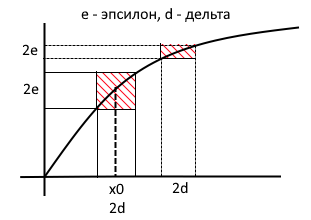
\includegraphics{3.9.1.png}
    \end{center}
    \underline{Примеры:}
    \begin{enumerate}
        \item $f(x) = x, x \in R$\\
        Пусть $x', x'' \in R : |x' - x''| < \delta$
        \[
            |f(x') - f(x'')| = |x' - x''| < \delta = \varepsilon
        \]
        \begin{center}
            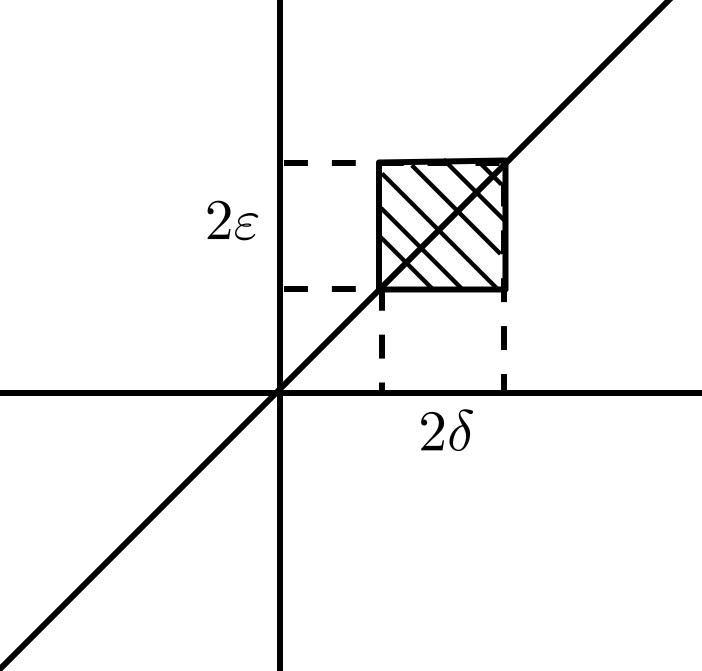
\includegraphics{3.9.2.png}
        \end{center}
        \item $f(x) = x^2, x \in R$\\
        Пусть $x', x'' \in R : |x' - x''| < \delta$\\
        Пусть $x'' = x' + h \implies |x' - x' - h| = |h| < \delta$
        \[ |f(x') - f(x'')| = |x'^2 - (x' + h)^2| = |x'^2 - x'^2 - 2x'h - h^2| = |2x'h + h^2| \]
        Так как $x' \in R$, то можно так его выбрать, что $|2x'h + h^2| = \infty \implies$ функция $f(x) = x^2$ не является непрерывной на области своего определения.
    \end{enumerate}
    \subsubsection*{Теорема 3.9.1 (Теорема Кантера)}\label{th:3.9.1}
    Если функция определена и непрерывна на отрезке $[a; b]$, то она равномерно-непрерывна на нём.\par\noindent
    \underline{Доказательство:}
    \begin{adjustwidth}{1.5em}{1.5em}
        Предположим противное. Пусть \[\forall \varepsilon > 0 \text{ } \exists \text{ } \delta = \delta(\varepsilon) : \forall x', x'' \in [a;b] :  |x' - x''| < \delta \implies |f(x') - f(x'')| \ge \varepsilon \]
        Зададим последовательность $\delta_n : \lim_{n\to\infty} \delta_n = 0$.\\
        Построим две вспомогательные последовательности $x_n'$ и $x_n''$:
        \[ \exists \text{ } x_1', x_1'' : |x_1' - x_1''| < \delta_1 \implies |f(x_1') - f(x_1'')| \ge \varepsilon \]
        \[ \exists \text{ } x_2', x_2'' : |x_2' - x_2''| < \delta_2 \implies |f(x_2') - f(x_2'')| \ge \varepsilon \]
        \[ \exists \text{ } x_n', x_n'' : |x_n' - x_n''| < \delta_n \implies |f(x_n') - f(x_n'')| \ge \varepsilon \]
        Рассмотрим $\posl{x'}{n}$: она ограничена. Тогда по \hyperref[th:2.8.1]{теореме Больцано-Вейерштрасса} из неё можно извлечь сх-ся подпосл-ть $\posl{x'}{n_k}$.\\
        Пусть $\lim_{k\to\infty} x'_{n_k} = x_0$\\
        Аналогично м. извлечь $\posl{x''}{n_k}$\\
        Т.к. $|x_n' - x_n''| < \delta_n \implies |x_{n_k}' - x_{n_k}''| < \delta_{n_k}$\\
        $\lim_{k\to\infty}x_{n_k}' = \lim_{k\to\infty}x_{n_k}'' = x_0$\\
        Так как $f(x)$ непрерывна на $[a; b]$, то она непрерывна в точке $x_0 \in [a;b]$\\
        Значит $\lim_{k\to\infty}f(x'_{n_k}) = \lim_{k\to\infty}f(x''_{n_k}) = f(x_0)$\\
        Рассмотрим $|f(x') - f(x'')| \ge \varepsilon \indent \circledast$
        \begin{adjustwidth}{1.5em}{1.5em}
            Перейдем в $\circledast$ к пределу при $k \to \infty$
            \[ \varepsilon \le | \lim_{k\to\infty}f(x'_{n_k}) - \lim_{k\to\infty}f(x''_{n_k})| = |f(x_0) - f(x_0)| = 0 \]
            Получили противоречие, т.к. $\varepsilon > 0 \implies f(x)$ - непрерывна.
        \end{adjustwidth}
    \end{adjustwidth}
    \underline{Пример:} рассмотрим $g = \sin \frac{1}{x}, x \in (0; 1)$
    \begin{adjustwidth}{1.5em}{1.5em}
        На $(0; 1)$ $y$ является непрерывна. Покажем, что на $(0; 1)$ $y$ не является равномерно-непрерывной функцией.\\
        Рассмотрим $x'_n$:
        \[x'_n = \frac{1}{\pi n}, \lim_{n\to\infty} x'_n = 0, x_n' \in (0; 1)\]
        Рассмотрим $x''_n$: 
        \[x''_n = \frac{1}{\frac{\pi}{2}+2\pi n}, \lim_{n\to\infty}x_n'' = 0, x''_n \in (0; 1)\]
        Рассмотрим 
        \[|f(x_n') - f(x_n'')| = |\sin \pi n - \sin (\frac{\pi}{2} + 2\pi n)| = 1\]
        \[ \forall \delta : |x_n' - x_n''| < \delta \implies |f(x'_n) - f(x''_n)| = 1 \]
        \[ \forall \varepsilon : 0 < \varepsilon < 1 \implies \nexists \delta(\varepsilon) \]
        Пусть $\varepsilon = \frac{1}{2}$. Тогда $\delta(\varepsilon) = \nexists$.
        \begin{center}
            \textbf{Ч.т.д.}
        \end{center}
    \end{adjustwidth}
    \underline{Замечание:} на практике, как правило, функции, которые растут больше, чем $y=x$, не является равн.-непр-ми на $D(f)$.



    \section{Дифференциальные исчисления функции}
    \subsection{Производная функции в точке}
    \noindent $y = f(x)$\\
    $\Delta x$ - приращение аргумента\\
    $\Delta y = f(x_0 + \Delta x) - f(x_0)$ - приращение функции\par\noindent
    \textbf{Производной} от функции $f(x)$ в точке $x_0$ называется предел отношения приращения функции в точке $x_0$ к приращению аргумента при стремлении последнего к 0.
    \[ \lim_{\Delta x \to 0} \frac{\Delta y}{\Delta x} = \lim_{\Delta x \to 0} \frac{f(x_0 + \Delta x) - f(x_0)}{\Delta x} = y' = \frac{dy}{dx} = \frac{d\sqcup}{dx}f \]
    \[ y'''' = y^{IV} = y^{(4)}  \]
    \underline{Замечание:} для существования производной от $f(x)$ в точке $x_0$ необходимо, чтобы $f(x)$ была определена в некоторой окрестности $x_0$ и в самой точке $x_0$.\\
    \underline{Замечание:} функция имеет производную в точке $x_0$, если $\exists$ $\lim_{\Delta x \to 0} \frac{\Delta y}{\Delta x}$\\
    \underline{Замечание:} если $\lim_{\Delta x \to 0}\frac{\Delta y}{\Delta x} = \pm \infty$, то говорят, что функция имеет бесконечную производную в точке.\par\noindent
    Если $\Delta x \to 0$ принимает только положительные значения то соответствующий предел называется правой производной от $f(x)$ в точке $x_0$.\\
    Если $\Delta x \to 0$ принимает только отрицательные значения то соответствующий предел называется левой производной от $f(x)$ в точке $x_0$.\par\noindent
    Функция $f(x)$ имеет производную на $[a; b]$, если она имеет производную во всех точках $(a; b)$, в точке $x=a$ имеет правую производную, в точку $x=b$ - левую.\par\noindent
    \underline{Утверждение:} если $f(x)$ имеет в точке $x_0$ правую и левую производные, то $f(x)$ имеет в точке $x_0$ производную.\\
    \underline{Утверждение:} если правая и левая производные в точке $x_0$ $\exists$ и не равны между собой, то производная в точке $x_0$ $\exists$.\\
    \underline{Пример:}
    \begin{adjustwidth}{1.5em}{1.5em}
        \begin{center}
            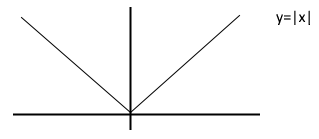
\includegraphics{4.1.1.png}
        \end{center}
        \[ \begin{matrix}
            y'\\
            \\
        \end{matrix}\Big|\begin{matrix}
            \\
            x = 0
        \end{matrix} \]
        Правая производная
        \[ \begin{matrix}
            y'_+\\
            \\
        \end{matrix}\Big|\begin{matrix}
            \\
            x = 0
        \end{matrix} = \lim_{\Delta x \to 0}\frac{f(x_0) - f(0)}{x_0 - 0} = \begin{vmatrix}
            \Delta x \to 0 \sim x_0 \to 0\\
            \\
            \\
        \end{vmatrix} = \lim_{x_0 \to 0} \frac{x_0 - 0}{x_0} = 1 \]
        Левая производная
        \[ \begin{matrix}
            y'_-\\
            \\
        \end{matrix}\Big|\begin{matrix}
            \\
            x = 0
        \end{matrix} = \lim_{\Delta x \to 0}\frac{f(-x_0) - f(0)}{-x_0 - 0} = \begin{vmatrix}
            \Delta x \to 0 \sim x_0 \to 0\\
            \\
            \\
        \end{vmatrix} = \lim_{x_0 \to 0} \frac{-x_0 - 0}{-x_0} = -1 \]
        Функция $y = |x|$ не имеет производной в точке 0.
    \end{adjustwidth}
    \underline{Пример:} докажем, что $y = x^2$ имеет производную в точке $x=0$.
    \begin{adjustwidth}{1.5em}{1.5em}
        \begin{center}
            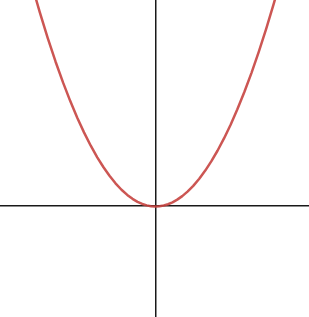
\includegraphics{4.1.2.png}
        \end{center}
        \begin{gather*}
            \lim_{x \to 0+0}\frac{f(x) - f(x_0)}{\Delta x} = \lim_{x\to 0+0} \frac{x^2 - 0}{x - 0} = 0\\
            \lim_{x \to 0-0}\frac{f(-x) - f(x_0)}{\Delta x} = \lim_{x\to 0-0} \frac{x^2 - 0}{-x-0} = 0
        \end{gather*}
        В точке $x = 0$ действительно $f'(x) = 0$.
        \begin{center}
            \textbf{Ч.т.д.}
        \end{center}
    \end{adjustwidth}
    
    \subsubsection*{Теорема 4.1.1}\label{th:4.1.1}
    Функция, имеющая конечную производную в точке, непрерывна в этой точке.\par\noindent
    \underline{Доказательство:}
    \begin{adjustwidth}{1.5em}{1.5em}
        Пусть существует $\lim_{x\to x_0} \frac{\Delta y}{\Delta x} = f'$ конечное.
        \[ \frac{\Delta y}{\Delta x} = f' + \varepsilon(\Delta x), \lim_{\Delta x \to 0}\varepsilon(\Delta x) = 0 \]
        \[ \Delta y = f' \Delta x + \varepsilon(\Delta x)\Delta x \]
        \[ \lim_{\Delta x \to 0} \Delta y = \lim_{\Delta x \to 0} (f' \Delta x + \varepsilon(\Delta x)\Delta x) = \lim_{\Delta x \to 0} f'\Delta x + \lim_{\Delta x \to 0} \varepsilon(\Delta x)\Delta x = 0 + 0 = 0 \]
        \begin{center}
            \textbf{Ч.т.д.}
        \end{center}
    \end{adjustwidth}

    \subsubsection*{Некоторые приложения производной}
    \begin{enumerate}
        \item Мгновенная скорость\par\noindent
        Пусть $S = S(t)$ - закон движения в точке.\\
        Рассмотрим $[ t, t + \Delta t ]$: $\Delta S = S(t+\Delta t) - S(t)$ - путь, пройденный за промежуток времени $\Delta t$.\\
        $v_{\text{ср}} = \frac{\Delta S}{\Delta t}$ - средняя скорость.\\
        Мгновенная скорость $v = \lim_{\Delta t \to 0} \frac{\Delta S}{\Delta t} = S'(t)$\\
        $a = \lim_{\Delta t \to 0} \frac{\Delta v}{\Delta t}$ - ускорение.    
    \end{enumerate}

    \subsection{Геометрический смысл производной}
    \begin{center}
        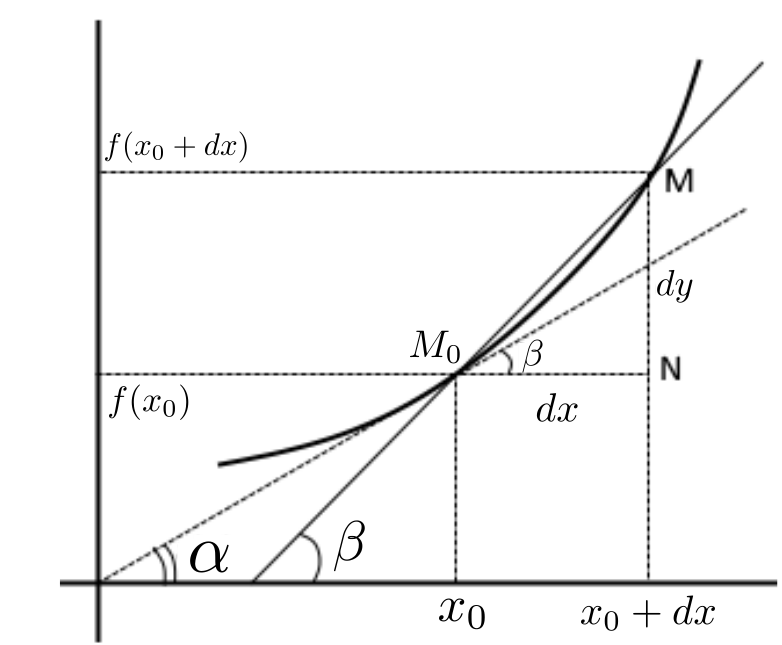
\includegraphics{4.2.1.png}
    \end{center}
    \[ M_0(x_0; f(x_0)) \]
    \[ M(x_0 + \Delta x; f(x_0 + \Delta x)) \]
    Запишем уравнение прямой $M_0M$\\
    \underline{Замечание:} уравнение прямой, проходящей через точки $(x_0; y_0)$ и $(x_1; y_1)$:
    \[ \frac{x - x_0}{x_1 - x_0} = \frac{y - y_0}{y_1 - y_0} \]
    \begin{gather*}
        \frac{x - x_0}{x_0 + \Delta x - x_0} = \frac{y - f(x_0)}{f(x_0 + \Delta x) - f(x_0)}\\
        \frac{x - x_0}{\Delta x} = \frac{y - y_0}{\Delta y}\\
        \Delta y(x - x_0) = \Delta x(y - y_0) \text{ } \big| \text{ } * \Delta x\\
        y - y_0 = \frac{\Delta y}{\Delta x}(x - x_0)\\
        y = \frac{\Delta y}{\Delta x}(x - x_0) + f(x_0) \text{ } \big| \text{ } : M_0M\\
        \tg  \angle \beta = \frac{|MN|}{|M_0N|} = \frac{\Delta y}{\Delta x}
    \end{gather*}
    Пусть $\Delta x \to 0$. Тогда точка $M$ будет стремиться к точке $M_0$, а угол $\beta$ к углу $\alpha$.
    \[ \lim_{\Delta x \to 0} \frac{\Delta y}{\Delta x} = f'(x_0) \text{ по определению} \]
    С другой стороны,
    \[ \lim_{\Delta x \to 0} \frac{\Delta y}{\Delta x} = \lim_{\Delta x \to 0} \tg  \beta = tg \lim_{\Delta x \to 0} \beta = tg \alpha \]
    Рассмотрим уравнение секущей при $\Delta x \to 0$
    \[ y = f'(x_0)(x - x_0) + f(x_0) \]
    \begin{center}
        - уравнение касательной к графику функции $f(x)$ в точке $x_0$.
    \end{center}

    Допустим $f'(x_0) = \infty$. Тогда рассмотрим уравнение секущей:
    \begin{gather*}
        y = \frac{\Delta y}{\Delta x} (x-x_0) + y_0 \text{ } \big| \text{ } : \frac{\Delta y}{\Delta x}\\
        \frac{y}{\frac{\Delta y}{\Delta x}} = x - x_0 + \frac{y_0}{\frac{\Delta y}{\Delta x}}
    \end{gather*}
    Перейдём к пределу при $\Delta x \to 0$. Тогда уравнение касательной примет вид \underline{$x = x_0$}.\par\noindent
    \underline{Замечание:} если $L_1 \perp L_2$
    \[ \begin{matrix}
        L_1: y = k_1x + b_1\\
        L_2: y = k_2x + b_2
    \end{matrix} \implies k_1k_2 = -1 \]
    Прямая, проходящая через точку $x_0$ перпендикулярно касательной, проведённой в этой точке, называется \underline{нормалью} к графику функции $f(x)$.
    \[ K_\text{н} = -\frac{1}{K_\text{кас}} = -\frac{1}{f'(x_0)} \]
    \[ y = -\frac{1}{f'(x_0)}(x - x_0) + y_0 \text{ (уравнение нормали)} \]

    \subsection{Производные элементарных функций}
    \begin{enumerate}
        \item $y = \mathbb{C} = const$\\
        $y(x) = \mathbb{C}, y(x + \Delta x) = \mathbb{C}$
        \[ y' = \lim_{\Delta x \to 0}\frac{y(x+ \Delta x) - y(x)}{\Delta x} = \lim_{\Delta x \to 0}\frac{\mathbb{C} - \mathbb{C}}{\Delta x} = 0 \]
        \item $y = \sin x$
        \[ y' = \lim_{\Delta x \to 0} \frac{\sin(x + \Delta x) - \sin x}{\Delta x} = \lim_{\Delta x \to 0}\frac{2\sin \frac{\Delta x}{2} * \cos (x + \frac{\Delta x}{2})}{\frac{\Delta x}{2} * 2} = \cos x \]
        Аналогично доказывается, что $(\cos x)' = - \sin x$
        \item $y = \log_{a}x$
        \[ \Delta y = \log_a(x+\Delta x) - \log_a(x) \]
        \[ \frac{\Delta y}{\Delta x} = \frac{\log_a(x+\Delta x) - \log_a(x)}{\Delta x} = \frac{\log_a\left(\frac{x+\Delta x}{x}\right)}{\Delta x} = \frac{1}{\Delta x} \log_a\left(1 + \frac{\Delta x}{x}\right) = \log_a\left(1+\frac{\Delta x}{x}\right)^{\frac{1}{\Delta x}} \]
        \begin{multline*}
            \lim_{\Delta x \to 0}\frac{\Delta y}{\Delta x} = \lim_{\Delta x \to 0} \log_a\left(1 + \frac{\Delta x}{x}\right)^{\frac{1}{\Delta x}} = \log_a\left(\lim_{\Delta x \to 0}\left(1 + \frac{\Delta x}{x}\right)^{\frac{1}{\Delta x} * \frac{x}{x}}\right) =\\
            = \log_a e^\frac{1}{x} = \frac{1}{x}\log_a e = \frac{1}{x\ln a} = (log_a x)'
        \end{multline*}
        \[ (\ln x)' = \frac{1}{x} \]
        \item $y = \tg (x) = \frac{\sin x}{\cos x}$
        По \hyperref[th:4.4.3]{теореме 4.4.3}
        \[ y' = \frac{(\sin x)'\cos x - (\cos x)'\sin x}{\cos^2 x} = \frac{\cos^2 x + \sin^2 x}{\cos^2 x} = \frac{1}{\cos^2 x} \]
        Аналогично доказывается, что $(\ctg  x)' = -\frac{1}{\sin^2 x}$
        \item $y = a^x$\\
        $x = \log_a y$ - обратная функция.
        \[ y'_x = \frac{1}{x'_y} \]
        \[ (a^x)'_x = \frac{1}{(\log_a y)'_y} = \frac{1}{\frac{1}{y\ln a}} = y \ln a = a^x \ln a \]
        \item $y = \arcsin x$\\
        $x = \sin y$
        \[ y'_x = \frac{1}{x'_y} \]
        \[ (\arcsin x)'_x = \frac{1}{(\sin y)'_y} = \frac{1}{\cos y} = \frac{1}{\sqrt{1 - \sin^2 y}} = \frac{1}{\sqrt{1 - \sin^2 (\arcsin x)}} = \frac{1}{\sqrt{1-x^2}} \]
        Аналогично: \begin{itemize}
            \item $(\arccos x)' = -\frac{1}{\sqrt{1-x^2}}$
            \item $(\arctg x)' = \frac{1}{1 + x^2}$
            \item $(\arcctg x)' = -\frac{1}{1+x^2}$
        \end{itemize}
        \item $y = x^\alpha = e^{\alpha \ln x}$
        По \hyperref[th:4.5.1]{теореме 4.5.1}
        \[ (x^\alpha)' = (e^{\alpha\ln x})' = e^{\alpha \ln x} * \alpha * \frac{1}{x} = x^\alpha * \alpha * \frac{1}{x} = \alpha * x^{\alpha - 1} \]
    \end{enumerate}
    \subsubsection*{Таблица производных}
    \begin{enumerate}
        \item $(x^n)' = nx^{n-1}$
        \item $(a^x)' = a^x \ln a$
        \item $(e^x)' = e^x$
        \item $(\log_ax)' = \frac{1}{x\ln a}$
        \item $(\ln x)' = \frac{1}{x}$
        \item $(\sin x)' = \cos x$
        \item $(\cos x)' = -\sin x$
        \item $(\tg x)' = \frac{1}{\cos^2 x}$
        \item $(\ctg x)' = -\frac{1}{\sin^2 x}$
        \item $(\arcsin x)' = \frac{1}{\sqrt{1 - x^2}}$
        \item $(\arccos x)' = -\frac{1}{\sqrt{1 - x^2}}$
        \item $(\arctg x)' = \frac{1}{1 + x^2}$
        \item $(\arcctg x)' = -\frac{1}{1 + x^2}$
        \item $(\sh x)' = \ch x$
        \item $(\ch x)' = \sh x$
        \item $(\th x)' = \frac{1}{\ch ^2 x}$
        \item $(\cth x)' = -\frac{1}{\sh ^2 x}$
    \end{enumerate}

    \subsection{Производная суммы, произведения, частного}
    \subsubsection*{Теорема 4.4.1}\label{th:4.4.1}
    \[ (u \pm v)' = u' \pm v' \]
    \noindent\underline{Доказательство:}
    \begin{adjustwidth}{1.5em}{1.5em}
        Рассмотрим \[y(x) = u(x) + v(x)\]
        \[\Delta y = u(x + \Delta x) + v(x + \Delta x) - u(x) - v(x)\]
        \[\frac{\Delta y}{\Delta x} = \frac{u(x+\Delta x) - u(x)}{\Delta x} + \frac{v(x + \Delta x) - v(x)}{\Delta x}\]
        \[ \lim_{\Delta x \to 0} \frac{\Delta y}{\Delta x} = \lim_{\Delta x \to 0}\frac{u(x+\Delta x) - u(x)}{\Delta x} + \lim_{\Delta x \to 0}\frac{v(x + \Delta x) - v(x)}{\Delta x} = u'(x) + v'(x)\]
        \begin{center}
            \textbf{Ч.т.д.}
        \end{center}
    \end{adjustwidth}
    \subsubsection*{Теорема 4.4.2}\label{th:4.4.2}
    \[ (uv)' = u'v + uv' \]
    \underline{Доказательство:}
    \begin{adjustwidth}{1.5em}{1.5em}
        Рассмотрим \[ y(x) = u(x)v(x) \]
        \[ \Delta y = u(x+\Delta x)v(x+\Delta x) - u(x)v(x) + u(x)v(x + \Delta x) - u(x)v(x + \Delta x) \]
        \[ \frac{\Delta y}{\Delta x} = \frac{[u(x+\Delta x) - u(x)]v(x+\Delta x)}{\Delta x} + \frac{u(x)[v(x+\Delta x)-v(x)]}{\Delta x} \]
        \[ \lim_{\Delta x \to 0}\frac{\Delta y}{\Delta x} = \lim_{\Delta x \to 0}\frac{[u(x+\Delta x) - u(x)]v(x+\Delta x)}{\Delta x} + \lim_{\Delta x \to 0}\frac{u(x)[v(x+\Delta x)-v(x)]}{\Delta x} = u'v + uv' \]
        \begin{center}
            \textbf{Ч.т.д.}
        \end{center}
    \end{adjustwidth}

    \subsubsection*{Теорема 4.4.3}\label{th:4.4.3}
    \[ \left(\frac{u}{v}\right)' = \frac{u'v - uv'}{v^2} \]
    \underline{Доказательство:}
    \begin{adjustwidth}{1.5em}{1.5em}
        Рассмотрим \[ y(x) = \frac{u(x)}{v(x)} \]
        \[ \Delta y = \frac{u(x + \Delta x)}{v(x + \Delta x)} - \frac{u(x)}{v(x)} = \frac{u(x + \Delta x)v(x) - u(x)v(x+\Delta x) + u(x)v(x) - u(x)v(x)}{v(x+\Delta x)v(x)} \]
        \[ \lim_{\Delta x \to 0}\frac{\Delta y}{\Delta x} = \lim_{\Delta x \to 0} \frac{[u(x + \Delta x) - u(x)]v(x) - u(x)[v(x+\Delta x) - v(x)]}{v(x+\Delta x)v(x)\Delta x} = \frac{u'v - uv'}{v^2} \]
        \begin{center}
            \textbf{Ч.т.д.}
        \end{center}
    \end{adjustwidth}

    \subsection{Производная сложной функции}
    Пусть функция $y = f(x)$ задана в некоторой окрестности точки $x_0 = u(x_0)$, а функция $z = g(y)$ - в некоторой окрестности $v = v(y_0)$ точки $y_0 = f(x_0)$, причём $f(u) \subset v$.\\
    Тогда определена сложная функция $F(x) = g(f(x))$.
    \subsubsection*{Теорема 4.5.1}\label{th:4.5.1}
    Если функция $y=f(x)$ имеет производную в точке $x_0$, а функция $z = g(y)$ имеет производную в точке $y_0 = f(x_0)$, то сложная функция $z = F(x) = g(f(x))$ также имеет производную в точке $x_0$, причём
    \[ \begin{matrix}F(x)\\\\\end{matrix}\Big|\begin{matrix}\\x = x_0\\\end{matrix} = \begin{matrix}y'(y)\\\\\end{matrix}\Big|\begin{matrix}\\y = y_0\\\end{matrix} * \begin{matrix}f'(x)\\\\\end{matrix}\Big|\begin{matrix}\\x = x_0\\\end{matrix} \]
    \underline{Доказательство:}
    \begin{adjustwidth}{1.5em}{1.5em}
        $\Delta x = x-x_0$\\
        $\Delta y = y-y_0$\\
        $\Delta z = g(y) - g(y_0)$\\
        Т.к. функция $g(y)$ имеет производную в точке $y_0$, то
        \[ \exists \lim_{\Delta y \to 0} \frac{\Delta z}{\Delta y} = g'(y_0) \]
        То есть
        \[ \frac{\Delta z}{\Delta y} = g'(y_0) + \varepsilon(\Delta y) \]
        \[ \lim_{\Delta y \to 0} \varepsilon(\Delta y) = o\left(g'(y_0) = \begin{matrix}g'(y)\\\\\end{matrix}\Big|\begin{matrix}\\y = y_0\\\end{matrix}\right) * \Delta y \]
        \[ \Delta z = g'(y_0) * \Delta y + \varepsilon(\Delta y) * \Delta y \text{ } \big| \text{ } : \Delta x \]
        \[ \frac{\Delta z}{\Delta x} = g'(y_0) \frac{\Delta y}{\Delta x} + \varepsilon(\Delta y)\frac{\Delta y}{\Delta x} \]
        \underline{Замечание:} по условию функция $y = f(x)$ имеет производную в точке $x_0$. Тогда по \hyperref[th:4.1.1]{теореме 4.1.1} $y = f(x)$ непрерывна в точке $x_0$, т.е. малому приращению аргумента соответствует малое приращение функции, т.е. если $\Delta x \to 0 \implies \Delta y \to 0 \implies \varepsilon(\Delta y) \to 0$
        \[ \lim_{\Delta x \to 0}\frac{\Delta z}{\Delta x} = g'(y_0)f'(x_0) + 0*f'(x_0) = \begin{matrix}g'(y)\\\\\end{matrix}\Big|\begin{matrix}\\y = y_0\\\end{matrix} * \begin{matrix}f'(x)\\\\\end{matrix}\Big|\begin{matrix}\\x = x_0\\\end{matrix} \]
        \begin{center}
            \textbf{Ч.т.д.}
        \end{center}
    \end{adjustwidth}

    \subsection{Производная обратной функции}
    \subsubsection*{Теорема 4.6.1}\label{th:4.6.1}
    Если функция непрерывна и возрастает (строго монотонна) в окрестности точки $x_0$ и имеет в точке $x_0$ производную $f'(x_0) \ne 0$, тогда обратная функция $x = f^{-1}(y)$ имеет производную в точке $y_0 = f(x_0)$ и \[ x'_y = \frac{1}{y'_x} \]
    \underline{Доказательство:}
    \begin{adjustwidth}{1.5em}{1.5em}
        \underline{Замечание 1:} если $f(x)$ возрастает и непрерывна в $u(x_0)$, то $f^{-1}(y)$ тоже возрастает и непрерывна на интервале $v = f(u)$\\
        \underline{Замечание 2:} функция $y = f(x)$ непрерывна в точке $x_0 \implies$ при $\Delta x \to 0 \implies \Delta y \to 0$\\
        \underline{Замечание 3:} т.к. $y = f(x)$ возрастает, то при $\Delta x \ne 0 \implies \Delta y \ne 0$\par\noindent
        Рассмотрим
        \[ x'_y = \lim_{\Delta y \to 0}\frac{\Delta x}{\Delta y} \overset{\text{ЗМ 2}}{=} \lim_{\Delta x \to 0}\frac{\Delta x}{\Delta y} \overset{\text{ЗМ 3}}{=} \lim_{\Delta x \to 0} \frac{1}{\frac{\Delta y}{\Delta x}} = \frac{1}{\lim_{\Delta x \to 0}\frac{\Delta y}{\Delta x}} = \frac{1}{y'_x} \]
        \begin{center}
            \textbf{Ч.т.д.}
        \end{center}
    \end{adjustwidth}

    \subsection{Гиперболические функции и их производные}
    \begin{enumerate}
        \item Гиперболический синус\\
        \[ \sh x = \frac{e^x - e^{-x}}{2} \]
        \begin{center}
            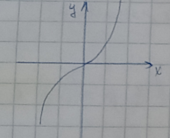
\includegraphics{4.7.1.png}\\
            $D(f) : R$\\
            $E(f) : R$\\
            нечётная, непрерывная, возрастает
        \end{center}
        \item Гиперболический косинус\\
        \[ \ch x = \frac{e^x + e^{-x}}{2} \]
        \begin{center}
            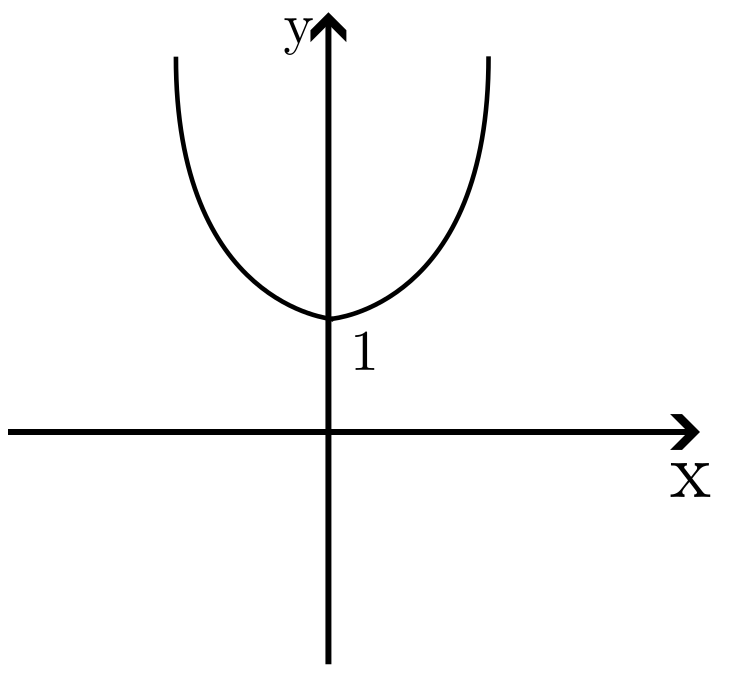
\includegraphics{4.7.2}\\
            $D(f) : R$\\
            $E(f) : [1; +\infty]$\\
            чётная, непрерывная
        \end{center}
        \item Гиперболический тангенс\\
        \[ \th x = \frac{\sh x}{\ch x} = \frac{e^x - e^{-x}}{e^x + e^{-x}} \]
        \begin{center}
            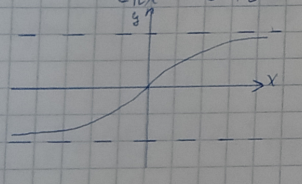
\includegraphics{4.7.3}\\
            $D(f) : R$\\
            $E(f) : (-1; 1)$\\
            нечётная, непрерывная, возрастающая
        \end{center}
        \item Гиперболический котангенс\\
        \[ \cth x = \frac{\ch x}{\sh x} = \frac{e^x + e^{-x}}{e^x - e^{-x}} \]
        \begin{center}
            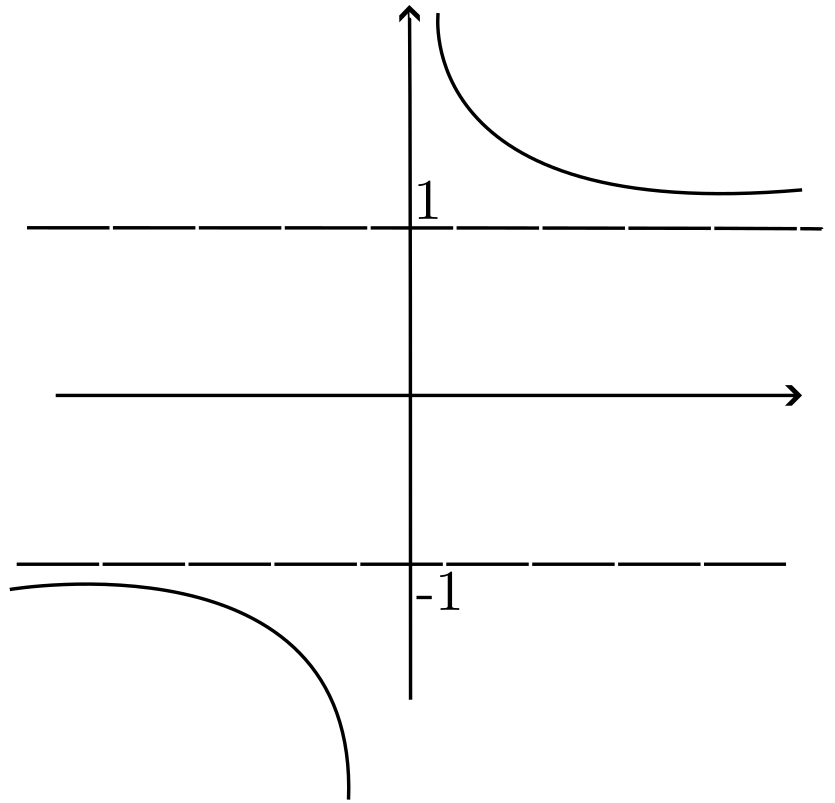
\includegraphics{4.7.4}\\
            $D(f) : R \backslash 0$\\
            $E(f) : (-\infty; -1) \cup (1; +\infty)$\\
            нечётная, в точке $x = 0$ разрыв II рода
        \end{center}
    \end{enumerate}
    \subsubsection*{Производные гиперболических функций}
    \begin{gather*}
        (\sh x)' = \left(\frac{e^x - e^{-x}}{2}\right)' = \frac{1}{2}(e^x + e^{-x}) = \ch x\\
        (\ch x)' = \left(\frac{e^x + e^{-x}}{2}\right)' = \frac{1}{2}(e^x - e^{-x}) = \sh x\\
        (\th x)' = \left(\frac{e^x - e^{-x}}{e^x + e^{-x}}\right)' = \frac{(e^x + e^{-x})(e^x + e^{-x}) - (e^x - e^{-x})(e^x - e^{-x})}{(e^x + e^{-x})^2} = \frac{e^{2x} + 2 + e^{-2x} - e^{2x} + 2 - e^{-2x}}{(e^x + e^{-x})^2} =\\
            = \frac{4}{(e^x + e^{-x})^2} = \frac{1}{\frac{(e^x + e^{-x})^2}{4}} = \frac{1}{\left(\frac{e^x + e^{-x}}{2}\right)^2} = \frac{1}{\ch^2 x}\\
        (\cth x)' \overset{\text{аналогично}}{=} -\frac{1}{\sh^2 x}
    \end{gather*}

    \subsection{Логарифмическое дифференцирование, производная от функции, заданной неявно, производная от функции, заданной параметрически}
    \begin{enumerate}
        \item \underline{Производная от функции, заданной неявно}\\
        $y = f(x)$ - явное задание функции\\
        \underline{Пример:}
        \begin{adjustwidth}{1.5em}{1.5em}
            $3x^4y^3 + 5x^3y^5 - 5 = 0$ - уравнение, определяющее неявно функцию $y = y(x)$\\
            $(x)' = 1$; $(y)' = y'$\\
            \[ 3(4x^3y^3 + x^4 * 3y^2 * y') + 5(3x^2y^5 + x^3*5y^4*y') = 0 \]
            \[ y'(9x^4y^2 + 25x^3y^4) = -12x^3y^3 - 15x^2y^5 \]
            \[ y' = \frac{-12x^3y^3 + 15x^2y^5}{9x^4y^2 + 25x^3y^4} \]
        \end{adjustwidth}
        \item \underline{Производная от функции, заданной параметрически}\\
        $\begin{cases}
            x = x(t)\\
            y = y(t)
        \end{cases}$\\
        $y = y(x)$\\
        \[ y'_x = \frac{dy}{dt} * \frac{dt}{dx} \overset{\hyperref[th:4.6.1]{\text{Th 4.6.1}}}{=} \frac{\frac{dy}{dt}}{\frac{dx}{dt}} = \frac{y'_t}{x'_t} \]
        \underline{Пример:}
        \begin{adjustwidth}{1.5em}{1.5em}
            $\begin{cases}
                x = 2\cos t\\
                y = 2\sin t
            \end{cases}$, $0 \le t \le 2\pi$\\
            $x'_t = -2\sin t$\\
            $y'_t = 2\cos t$
            \[ y'_x = \frac{2\cos t}{-2\sin t} = -\ctg t \]
        \end{adjustwidth}
        \item \underline{Логарифмическое дифференцирование}\\
        $y = u(x)^{v(x)}$ - степенно-показательная функция
        \begin{enumerate}
            \item \underline{Логарифмическое дифференцирование}\\
            \[ y = u(x)^{v(x)} \]
            \[ \ln y = \ln u(x)^{v(x)} \]
            \[ \ln y = v(x) * \ln u(x) \]
            \[ \frac{1}{y} * y' = v'(x)\ln u(x) + v(x)\frac{1}{u(x)}*u'(x) \text{ } \big| \text{ } * y \]
            \[ y' = u(x)^{v(x)}\left[v'(x)\ln(u(x)) + \frac{v(x)}{u(x)} * u'(x)\right] \]
            \item \underline{Сведение к сложной функции}
            \[ y = u(x)^{v(x)} = \left|a = b^{\log_b a}\right| = e^{\ln u(x) * v(x)} \]
            \[ y' = e^{\ln u(x) * v(x)} * \left[ \frac{1}{u(x)} * u'(x)*v(x) + \ln(u(x)) * v'(x) \right] \]
            \item \begin{align*}
                y &= u(x) & y &= (u(x))^n & y &= a^{v(x)}\\
                &\vdots & y' &= n(u(x))^{n-1} * u'(x) & y' &= a^{v(x)} * \ln(a) * v'(x)
            \end{align*}
            \[ y' = v(x)u(x)^{v(x)-1} * u'(x) + u(x)^{v(x)} * \ln u(x) * v'(x) \]
        \end{enumerate}
    \end{enumerate}

    \subsection{Дифференцируемость функции. Дифференциал, его геометрический и физический смыслы}
    Функция $y = f(x)$, заданная в $u(x_0)$, называется дифференцируемой в этой точке, если её приращение $\Delta y = f(x_0 + \Delta) - f(x_0)$ представимо в этой окрестности в виде $\Delta y = A\Delta x + o(\Delta x)$, $\Delta \to 0$, $A = const$\par\noindent
    Линейная часть приращения функции $A\Delta x $ называется дифференциалом функции в точке $x_0$ и обозначается $\begin{matrix}df\\\\\end{matrix}\Big|\begin{matrix}\\x = x_0\\\end{matrix}$ или $df(x_0)$.\\
    Тогда $\Delta y = dy+o(\Delta x)$\par\noindent
    \underline{Замечание:} $o(\Delta x)=o(A\Delta x)=o(dy)$
    \begin{adjustwidth}{1.5em}{1.5em}
        Тогда $\Delta y = dy + o(dy)| : dy$\\
        $\frac{\Delta y}{dy}=1+\frac{o(dy)}{dy}$\\
        $\lim_{\Delta x \to 0}{\frac{\Delta y}{dy}}=1$\\
        Т.е. $\Delta y \sim dy $ при $\Delta x \to 0$
    \end{adjustwidth}

    \subsection*{Теорема 4.9.1 (необходимость и достаточность условия дифференции в точке)}\label{th:4.9.1}
    Для того чтобы $f(x)$ была дифференцируема в точке $x_0$ $\Leftrightarrow$ чтобы в этой точке она имела конечную производную.\par\noindent
    \underline{Доказательство:}
    \begin{adjustwidth}{1.5em}{1.5em}
        \textbf{Докажем необходимость ($\Rightarrow$)}\\
        Пусть $f(x)$ дифференцируема в точке $x_0$. Покажем, что $\exists$ $f'(x_0)$ - конечное.\\
        Тогда по определению 
        \begin{gather*}
            \Delta y = A \Delta x+o(\Delta x)\\
            \Delta y = A \Delta x+ \varepsilon(\Delta x)*\Delta x\\
            \lim_{\Delta x \to 0}{\varepsilon(\Delta x)}= 0\\
            \frac{\Delta y}{\Delta x}=A+\varepsilon(\Delta x)\\
            lim_{\Delta x \to 0}{\frac{\Delta y}{\Delta x}}=A\\
            f'(x)|x=x_0=A=const
        \end{gather*}
        \textbf{Докажем достаточность ($\Leftarrow$)}\\
        Пусть $f(x)$ имеет конечную производную в точке $x_0$, т.е. $\exists \lim_{\Delta x \to 0}{\frac{\Delta y}{\Delta x}}=f'(x_0)$\\
        \begin{gather*}
            \frac{\Delta y}{\Delta x}=f'(x_0)+\varepsilon(\Delta x)|*\Delta x\\
            \Delta y=f'(x_0)\Delta x+\varepsilon(\Delta x)\Delta x= f'(x_0)\Delta x+o(\Delta x)    
        \end{gather*}
        \begin{center}
            \textbf{Ч.т.д.}
        \end{center}    
    \end{adjustwidth}
    \underline{Замечание:} таким образом $\begin{matrix}df\\\\\end{matrix}\Big|\begin{matrix}\\x = x_0\\\end{matrix}=f'(x_0)\Delta x$
    \subsubsection*{Геометрический смысл дифференциала}
    \begin{center}
        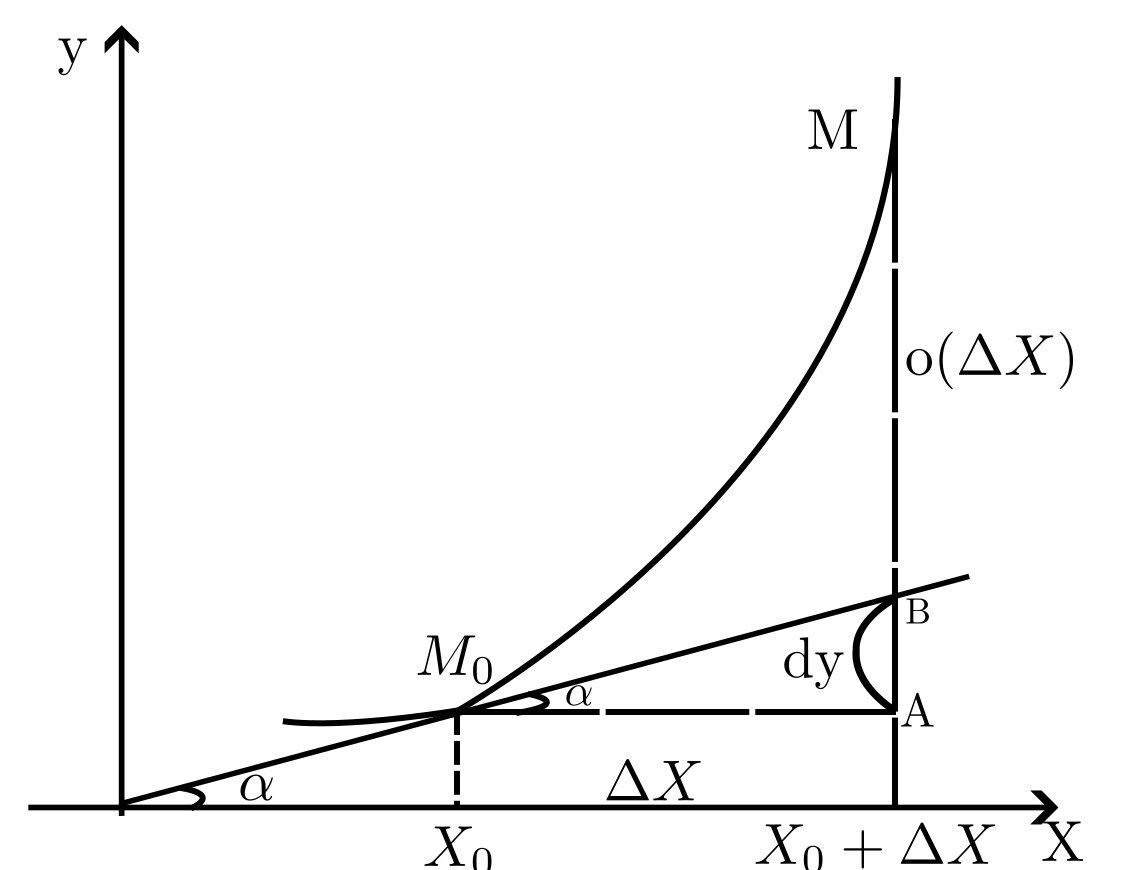
\includegraphics{4.9.1}
    \end{center}
    Рассмотрим функцию $y=f(x)$:
    \begin{gather*}
        M_0(x_0,f(x_0))\\
        M(x_0, \Delta x,f(x_0+\Delta x))\\
        \tg \alpha = f'(x_0)    
    \end{gather*}
    Рассмотрим $\Delta ABM_0$:
    \begin{gather*}
        \tg \alpha = |AB|\\
        f'(x_0)\Delta x = \Delta y\\
        |MB|=o(\Delta x)
    \end{gather*}
    \begin{center}
        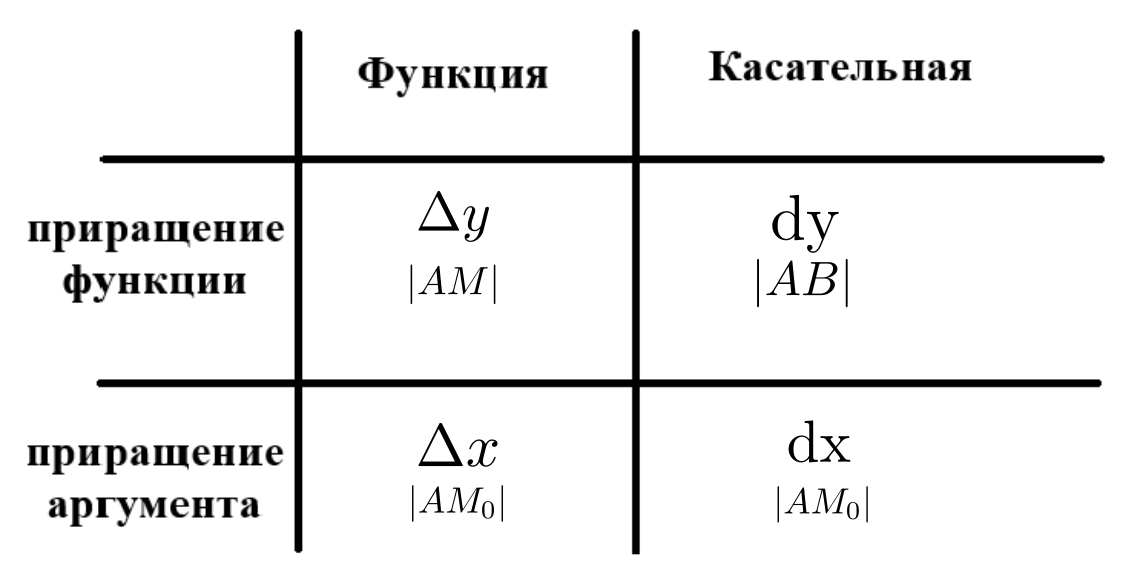
\includegraphics{4.9.2}
    \end{center}
    Отсюда для независимой переменной $x$: $\Delta x = dx$\\
    Геометрический смысл дифференциала: это есть приращение ординаты касательной, проведённой к графику функции в точке $x_0$.\par\noindent
    \underline{Замечание:} для функции $y = kx+b$ $dy = \Delta y$ для любых $x$.\\
    \underline{Замечание:} $dy = \begin{matrix}f'(x)\\\\\end{matrix}\Big|\begin{matrix}\\x=x_0\\\end{matrix} * dx \implies \begin{matrix}f'(x)\\\\\end{matrix}\Big|\begin{matrix}\\x=x_0\\\end{matrix} = \frac{dy}{dx}$
    \subsubsection*{Физический смысл диффернциала}
    \[V_{\text{мгнов}}=\begin{matrix}S'(t)\\\\\end{matrix}\Big|\begin{matrix}\\t=t_0\\\end{matrix}=\frac{dS}{dt}\]
    \[ dS = \begin{matrix}S'(t)\\\\\end{matrix}\Big|\begin{matrix}\\t=t_0\\\end{matrix} * dt = \begin{matrix}S'(t)\\\\\end{matrix}\Big|\begin{matrix}\\t = t_0\\\end{matrix} * \Delta t \]
    Дифференциал $dS$ равен пути, который прошла бы рассматриваемая точка за время $\Delta t$, начиная с момента времени $t=t_0$, если бы на этом участке пути скорость была бы постоянной и равной $\begin{matrix}S'(t)\\\\\end{matrix}\Big|\begin{matrix}\\t=t_0\\\end{matrix}$
    \subsubsection*{Свойства дифферинциалов}
    \begin{enumerate}
        \item $d(u \pm V)=du \pm dv$
        \item $d(uv)=udv+vdu$
        \item $d(Cu)=Cdu$
        \item $d(\frac{u}{v})=\frac{u'v-uv'}{v^2}=\frac{vdu-udv}{v^2}$
    \end{enumerate} 
    \underline{Доказательство 4-го пункта:}
    \begin{adjustwidth}{1.5em}{1.5em}
        \[d\left(\frac{u}{v}\right)=\left(\frac{u}{v}\right)'dx=\frac{u'v-uv'}{v^2}dx=\frac{vdu-udv}{v^2}\]
        \begin{center}
            \textbf{Ч.т.д.}
        \end{center}
    \end{adjustwidth}
    \subsection{Примемение дифференциала в приближённых вычислениях. Дифференциал сложной функции}
    \noindent Если $f(x)$ дифференцируема в точке $x_0$
    \begin{adjustwidth}{1.5em}{1.5em}
        $\Delta y=dy+o(dx)$\\
        $\Delta y \approx dy$\\
        $f(x_0+\Delta x)-f(x_0) \approx f'(x_0) \Delta x$\\
        $f(x_0+\Delta x) \approx f(x_0)+f'(x_0) \Delta x$ - \textbf{формула приближённого вычисления функции}.
    \end{adjustwidth}
    \underline{Пример:} $\sin 32^\circ$
    \begin{adjustwidth}{1.5em}{1.5em}
        Рассмотрим $f(x)=\sin x$\\
        $32 = x_0+\Delta x=30 + 2$\\
        $x_0=30;\Delta x = 2 = \frac{\pi}{90}$\\
        $f'(x)=const$\\
        $f(30)=\frac{1}{2}$
        $f'(30)=\frac{\sqrt{3}}{2}$
        $sin 32 = \frac{1}{2}+\frac{\sqrt{3}}{2}-\frac{\pi}{90}=0,53$    
    \end{adjustwidth}

    \subsubsection*{Дифференцируемость сложной функции}
    \noindent Рассмотрим $y = f(x)$\\
    $z = g(y)$\\
    Получим $F(x) = g(f(x))$
    \[ \begin{matrix}F'(x)\\\\\end{matrix}\Big|\begin{matrix}\\x=x_0\\\end{matrix} = \begin{matrix}g'(y)\\\\\end{matrix}\Big|\begin{matrix}\\y=y_0\\\end{matrix} * \begin{matrix}f'(x)\\\\\end{matrix}\Big|\begin{matrix}\\x=x_0\\\end{matrix} \]
    Рассмотрим
    \[ dF = \begin{matrix}F'(x)\\\\\end{matrix}\Big|\begin{matrix}\\x=x_0\\\end{matrix}dx = \begin{matrix}g'(y)\\\\\end{matrix}\Big|\begin{matrix}\\y=y_0\\\end{matrix} * \begin{matrix}f'(x)\\\\\end{matrix}\Big|\begin{matrix}\\x=x_0\\\end{matrix}*dx = g'(y)dy \]
    Формула показывает, что записи дифференциала посредством независимой переменной $x$ и зависимой переменной $y$ имеет один и тот же вид.\\
    Это свойство называется \textbf{инвариантностью} формы записи первого дифференциала.

    \subsection{Производные дифференциалов высших порядков}
    \noindent Пусть $y = f(x)$ имеет производную $y' = f(x)$ во всех точках некоторой окрестности точки $x_0$.\\
    Если в свою очередь $f'(x)$ имеет производную $\begin{matrix}[f'(x)]'\\\\\end{matrix}\Big|\begin{matrix}\\x=x_0\\\end{matrix}$, то она называется второй производной функции $f(x)$ в точке $x_0$.\\
    Аналогично определяются производные более высоких порядков: $f^{(n)} = (f^{(n-1)})'$.\\
    \underline{Примеры:}
    \begin{enumerate}
        \item $y = a^x$\\
        $y' = a^x \ln a$\\
        $y'' = a^x \ln^2 a$\\
        $y^{(n)} = a^x \ln^n a$
        \item $y = \sin x$\\
        $y' = \cos x = \sin (\frac{1 \pi}{2} + x)$\\
        $y'' = - \sin x = \sin (\frac{2 \pi}{2} + x)$\\
        $y^{(n)} = \sin (\frac{n \pi}{2} + x)$
        \item $y = \cos x$\\
        $y^{(n)} = \cos (\frac{n \pi}{2} + x)$
        \item $y = \ln x$\\
        $y' = \frac{1}{x}$\\
        $y'' = -\frac{1}{x^2}$\\
        $y''' = \frac{1}{x^3}$\\
        $\vdots$\\
        $y^{(n)} = (-1)^{n-1} * \frac{(n-1)!}{x^n}$
        \item $y = x^n, n \in N$\\
        $y' = nx^{n-1}$\\
        $y'' = n(n-1)x^{n-2}$\\
        $\vdots$\\
        $y^{(k)} = n(n-1)\dots(n-k+1)x^{n-k}$\\
        $\vdots$\\
        $y^{(n)} = n!$
        \item $y = \lambda_1 y_1(x) + \lambda_2 y_2(x)$\\
        $y^{(n)} = \lambda_1 y_1^{(n)}(x) + \lambda_2 y_2^{(n)}(x)$
        \item $y = uv$\\
        $y' = u'v + uv'$\\
        $y'' = u''v + u'v' + u'v' + uv'' = u''v + 2u'v' + uv''$\\
        $y''' = u'''v + 3u''v' + 3u'v'' + uv'''$\\
        $\vdots$\\
        $y^{(n)} = \sum_{k=0}^{n} C^k_n u^{(k)} v^{(n-k)} = \sum_{k=0}^{n} C^k_n u^{(n-k)} v^{(k)}$ - \textbf{формула Лейбница}\\
        $(k), (n-k)$ - символическая степень (применяем формулу бинома Ньютона, но не возводим в степень, а берём производную)
    \end{enumerate}

    \subsubsection*{Производная высшего порядка от функции, заданной параметрически}
    \[ \begin{cases}
        x = x(t)\\
        y = y(t)
    \end{cases} \]
    \[ y'_x = y'_t * t'_x = \frac{y'_t}{x'_t} = A(t) \]
    \[ y''_{xx} = (y'_x)'_x = (A(t))'_t t'_x = \frac{(y'_x)'_t}{x'_t} = B(t) \]
    \[ y'''_{xxx} = (y''_{xx})'_x = (B(t))'_t t'_x = \frac{(y''_{xx})'_t}{x'_t} \]
    \[ \boxed{y^{(n)}_{\underbrace{x \dots x}_{n}} = \frac{(y^{(n-1)}_{\underbrace{x \dots x}_{n-1}})'_t}{x'_t}} \]
    \subsubsection*{Производная высшего порядка от функций, заданных неявно}
    \underline{Пример:} $x^2 + y^2 = 25$
    \[ 2x + 2yy' = 0 \]
    \begin{align*}
        x + yy' &= 0 & y' &= -\frac{x}{y}\\
        1 + yy'' + (y')^2 &= 0 & y'' &= -\frac{1+(y')^2}{y} = f_2(x;y)\\
        y'y'' + yy'' + 2y'y'' &= 0 & y''' &= -\frac{3y'y''}{y} = f_3(x; y)
    \end{align*}

    \subsubsection*{Дифференциалы высших порядков}
    \[ y = f(x) \]
    \[ dy = f'(x)dx \]
    Пусть функция $f'(x)$ также дифференциуема в точке $x_0$ и \textbf{величина} $dx$ \textbf{имеет одно и то же фиксированное значение} для $\forall x \in u(x_0)$\\
    Рассмотрим \[ d^2f(x) = d(df(x)) = d(f'(x)dx) = (f'(x)dx)'_x dx = f''(x)dxdx = f''(x)dx^2 \] 
    \[ dx^2 = (dx)^2 \text{ } (\text{дэ икс дважды}) \]
    \[ y'' = \frac{d^2y}{dx^2} \]
    Аналогично дифференциал порядка $n$ называется дифференциал от дифференциала порядка $(n-1)$ при условии, что $dx = const$, то есть 
    \[ d^ny = d(d^{n-1}y) = y^{(n)}dx^n \text{ (дэ икс эножды)} \]
    \underline{Замечание:} дифференциалы высших порядков $(n \ge 2)$ не обладают свойством инвариантности формы записи относительно выбора переменных.\\
    \underline{Доказательство:}
    \begin{adjustwidth}{1.5em}{1.5em}
        $y = f(x), z = z(y) \indent z = z(f(x))$ - сложная функция\\
        \begin{gather*}
            dz = z'_ydy\\
            d^2z = d(dz) = d(z'_y\underset{\text{не const}}{dy}) = \begin{vmatrix}
                d(uv) = udv + vdu\\
                \\
            \end{vmatrix} = z'_yd^2y + dyd(z'y) = z'_yd^2y + z''_{yy}dy^2\\
            z'_yd^2y = 0 \text{ для линейной функции}
        \end{gather*}
    \end{adjustwidth}

    \subsection{Дифференциальные теоремы о среднем}
    Точка $x = c$ называется точкой локального максимума (минимума) функкции $y = f(x)$, если $\exists u_\delta(c) : (c - \delta; c + \delta) : $\\
    \[ f(c) \ge f(x) \text{ } \forall x \in (c - \delta; c + \delta) \]
    \[ \left( f(c) \le f(x) \text{ } \forall x \in (c - \delta; c + \delta) \right) \]
    Точка локального максимума (минимума) функции называется точкой локального экстремума.
    \subsubsection*{Теорема 4.12.1 (Ферма)}\label{th:4.12.1}
    Если $f(x)$ имеет производную в точке $c$ и достигает в этой точке экстремум, то $f'(c) = 0$\par\noindent
    \underline{Доказательство:}
    \begin{adjustwidth}{1.5em}{1.5em}
        Пусть точка $c$ - точка локального экстремума.
        \[ f'(c) = \lim_{\Delta x \to 0} \frac{f(c+\Delta x) - f(c)}{\Delta x} \]
        Пусть для определённости точка $c$ - точка максимума ($f(c) \ge f(x) \forall x \in (c-\delta; c+\delta)$)\\
        Т.к. производная в точке $c$ существует, то существует 
        \begin{align*}
            \left.\begin{array}{r@{}l}
                f'_+(c) = \lim_{\Delta x \to 0}\frac{f(c+\Delta x) - f(c)}{\Delta x} \le 0\\
                f'_-(c) = \lim_{\Delta x \to 0}\frac{f(c+\Delta x) - f(c)}{\Delta x} \ge 0
            \end{array}\right\} \text{т.к. } f'(c) \exists \implies f'(c) = 0
        \end{align*}
        \begin{center}
            \textbf{Ч.т.д.}
        \end{center}
    \end{adjustwidth}
    \underline{Замечание:} точка, в которой функция достигает экстремальное значение, является внутренней точкой интервала.

    \subsubsection*{Теорема 4.12.2 (Ролля)}\label{th:4.12.2}
    Если $f(x)$ непрерывна на $[a; b]$, дифференциуема на $(a; b)$ и $f(a) = f(b)$. Тогда на $(a;b)$ $\exists$ по крайней мере одна точка $\xi \in (a; b) : f'(\xi) = 0$\par\noindent
    \underline{Доказательство:}
    \begin{adjustwidth}{1.5em}{1.5em}
        \begin{enumerate}
            \item $f = const$. Тогда $\forall \xi \in (a; b) f'(\xi) = 0$. \textbf{Ч.т.д.}
            \item $f \ne const$. Тогда по \hyperref[th:3.8.2]{второй теореме Вейерштрасса} существуют точки $x_1, x_2$, в которых функция достигает своих наибольшего и наименьшего значений. Причём обе точки $x_1$ и $x_2$ не могут быть концами $[a;b]$ одновременно. Т.к. $\underset{x\in [a;b]}{max f(x)} = \underset{x\in [a;b]}{min f(x)} = f(a) = f(b)$ по условию. Тогда $f(x)$ была бы константой, а это не так. Т.е. одна из $x_1, x_2 \in (a;b)$. Обозначим её $\xi$. По условию $f(x)$ дифференциуема на $(a;b) \overset{\hyperref[th:4.9.1]{\text{Th 4.9.1}}}{\implies} \exists$ конечная $f'(\xi)$. А так как в этой точке функция принимает наибольшее или наименьшее значение $\implies f'(\xi) = 0$.
        \end{enumerate}
        \begin{center}
            \textbf{Ч.т.д.}
        \end{center}
    \end{adjustwidth}

    \subsubsection*{Геометрический смысл теоремы Ролля}
    \begin{center}
        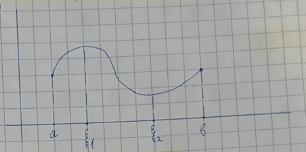
\includegraphics{4.12.1}
    \end{center}

    \subsubsection*{Теорема 4.12.3 (теорема Коши)}\label{th:4.12.3}
    Если функции $f(x)$ и $g(x)$ непрерывны на $[a;b]$, дифференциуемы на $(a;b)$, $g'(x) \ne 0 \text{ } \forall x \in (a;b)$. Тогда $\exists$ точка $\xi \in (a;b)$:
    \[ \frac{f(b) - f(a)}{g(b) - g(a)} = \frac{f'(\xi)}{g'(\xi)} \]
    \underline{Доказательство:}
    \begin{adjustwidth}{1.5em}{1.5em}
        \underline{Замечание:} $g(b) \ne g(a)$, так как, если бы это было так, то $g(x)$ удовлетворяла бы условию \hyperref[th:4.12.2]{теоремы Ролля} $\implies \exists$ точка $\xi \in (a;b) : g'(\xi) = 0$, а это не так.\par\noindent
        Составим вспомогательную функцию
        \[ F(x) = f(x) - f(a) - \frac{f(b) - f(a)}{g(b) - g(a)} * (g(x) - g(a)) \]
        Т.к. $f(x), g(x)$ непрерывны на $[a;b]$ и дифференциуемы на $(a;b) \implies F(x)$ непрерывна на $[a;b]$ и дифференциуема на $(a;b)$\\
        $F(a) = 0; F(b) = 0$\\
        Т.е. $F(x)$ удовлетворяет условию \hyperref[th:4.12.2]{теоремы Ролля} $\implies \exists$ точка $\xi \in (a;b) : F'(\xi) = 0$.\\
        Тогда:
        \[ F'(x) = f'(x) - \frac{f(b) - f(a)}{g(b) - g(a)} * g'(x) \]
        \[ F'(\xi) = 0 \implies f'(\xi) - \frac{f(b) - f(a)}{g(b) - g(a)} * g'(\xi) = 0 \]
        \[ \frac{f(b) - f(a)}{g(b) - g(a)} * g'(\xi) = f'(\xi) \text{ } \big| \text{ } * g'(\xi) \ne 0 \]
        \[ \frac{f(b) - f(a)}{g(b) - g(a)} = \frac{f'(\xi)}{g'(\xi)} \]
        \begin{center}
            \textbf{Ч.т.д.}
        \end{center}
    \end{adjustwidth}
    
    \subsubsection*{Теорема 4.12.4 (теорема Лагранжа)}\label{th:4.12.4}
    Если $f(x)$ непрерывна на $[a;b]$ и дифференциуема на $(a;b)$, тогда $\exists$ точка $\xi \in (a; b)$: 
    \[ \boxed{f(b) - f(a) = f'(\xi)(b-a)} \]
    \underline{Доказательство:}
    \begin{adjustwidth}{1.5em}{1.5em}
        Если в \hyperref[th:4.12.3]{теореме Коши} принять $g(x) = x \implies$ \textbf{ч.т.д.}\par\noindent
        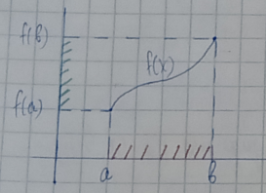
\includegraphics{4.12.2}
    \end{adjustwidth}

    \subsubsection*{Геометрический смысл теоремы Лагранжа}
    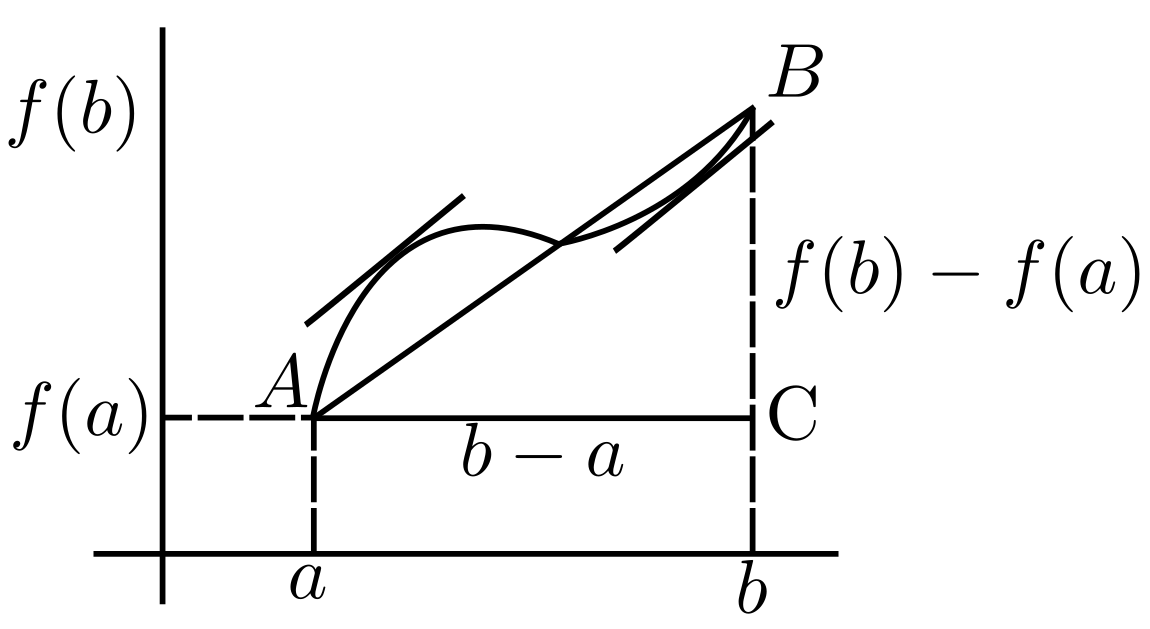
\includegraphics{4.12.3}
    \[ \frac{f(b) - f(a)}{b-a} = \tg \angle A = f'(\xi) \]
    $\exists$ точка $\xi \in (a;b)$ : касательная к графику функции в этой точке $\parallel$-на хорде $AB$\par\noindent
    \underline{Замечание:} промежуточное значение $\xi$ можно записать в виде $\xi = a + \theta(b-a), 0 < \theta < 1$\\
    Тогда
    \[ \boxed{ f(b) - f(a) = f'(a + \theta (b-a)) * (b-a) } \]
    Пусть $(b-a) = \Delta x$\\
    $f(b) - f(a) = f(x+\Delta x) - f(x)$\\
    Тогда
    \[ \boxed{ f(x+\Delta x) - f(x) = f'(x+\theta \Delta x) \Delta x } \]
    Все три формулы называются формулой конечных приращений Лагранжа.
    
    \subsubsection*{Теорема 4.12.5}\label{th:4.12.5}
    Если $f(x)$ непрерывна на $[a;b]$, дифференциуема на $(a;b)$ и $\forall x \in (a;b)$ $f'(x) = 0 \implies f(x)$ постоянная на этом отрезке.\par\noindent
    \underline{Доказательство:}
    \begin{adjustwidth}{1.5em}{1.5em}
        Выберем произвольно $x_1, x_2 \in [a; b]$. Пусть для определённости $x_1 < x_2$.\\
        Тогда $f(x)$ непрерывна $[x_1;x_2] \subset [a;b]$ и дифферецируема $(x_1; x_2) \subset (a; b)$.\\
        Тогда по \hyperref[th:4.12.4]{теореме Лагранжа} $f(x_2) - f(x_1) = f'(\xi)(x_2-x_1), x_1 < \xi < x_2$.\\
        По условию $f'(x) = 0$ $\forall x \in (a; b) \implies f'(\xi) = 0$, т.к. точка $\xi \in (x_1; x_2) \subset (a; b) \implies f(x_1) = f(x_2)$, а т.к. $x_1, x_2$ - произвольные и $\in [a; b]$, то $f(x) = const$ $\forall x \in [a;b]$.
        \begin{center}
            \textbf{Ч.т.д.}
        \end{center}
    \end{adjustwidth}

    \subsection{Раскрытие неопределённости по правилу Лопиталя}
    \subsubsection*{Теорема 4.13.1}\label{th:4.13.1}
    Если $f(x)$ и $g(x)$ определены в $u(x_0)$ и в этой точке $f(x_0) = g(x_0) = 0$, то
    \[ \lim_{x\to x_0}\frac{f(x)}{g(x)} = \left[\frac{0}{0}\right] = \frac{f'(x_0)}{g'(x_0)} = \frac{f'(x)}{g'(x)}\Big|_{x = x_0} \]
    \underline{Доказательство:}
    \begin{adjustwidth}{1.5em}{1.5em}
        \[ \lim_{x \to x_0}\frac{f(x)}{g(x)} = \lim_{x\to x_0}\frac{f(x) - f(x_0)}{g(x) - g(x_0)} = \lim_{x\to x_0} \frac{\frac{f(x)-f(x_0)}{x - x_0}}{\frac{g(x) - g(x_0)}{x - x_0}} = \frac{f'(x_0)}{g'(x_0)} \]
        \begin{center}
            \textbf{Ч.т.д.}
        \end{center}
    \end{adjustwidth}
    
    \subsubsection*{Геометрический смысл}
    \begin{center}
        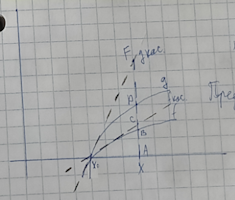
\includegraphics{4.13.1}
    \end{center}
    \[ \lim_{x\to x_0}\frac{|AB|}{|AO|} = \lim_{x\to x_0}\frac{|AC|}{|AF|} \]
    Предел отношения ординат графиков функции $f$ и $g$ равен пределу отношения касательных к этим функциям в точке $x_0$.

    \subsubsection*{Теорема 4.13.2}\label{th:4.13.2}
    \noindent Если: \begin{enumerate}
        \item Функции $f$ и $g$ дифференциуемы на $(a;b)$
        \item $g'(x) \ne 0$ $\forall x \in (a;b)$
        \item $\lim_{x\to a} f(x) = \lim_{x\to a}g(x) = 0$
        \item $\exists$ конечный или бесконечный $\lim_{x\to a} \frac{f'(x)}{g'(x)}$
    \end{enumerate}
    Тогда $\exists \lim_{x\to a}\frac{f(x)}{g(x)} = \lim_{x\to a}\frac{f'(x)}{g'(x)}$\par\noindent
    \underline{Доказательство:}
    \begin{adjustwidth}{1.5em}{1.5em}
        Так как по пункту 1 $f(x)$ и $g(x)$ дифференциуемы на $(a;b) \underset{\hyperref[th:4.1.1]{\text{Th 4.1.1}}}{\overset{\hyperref[th:4.9.1]{\text{Th 4.9.1}}}{\implies}}$ они непрерывны на $(a; b)$.\\
        Доопределим эти функции в точке $x = a$: $f(a) = g(a) = 0$.\\
        Тогда $\forall x \in (a; b)$ на $[a; x]$ $f(x)$ и $g(x)$ будут удовлетворять условию \hyperref[th:4.12.3]{теоремы Коши}, т.е. $\exists$ точка $\xi = \xi(x)$ и $\frac{f(x)}{g(x)} = \frac{f(x) - f(a)}{g(x) - g(a)} \overset{\hyperref[th:4.12.3]{\text{Th 4.12.3}}}{=} \frac{f'(\xi)}{g'(\xi)}$
        \[ \boxed{\lim_{x \to a}\frac{f(x)}{g(x)}} = \lim_{x\to a}\frac{f'(\xi)}{g'(\xi)} = \begin{vmatrix}
            a < \xi < x\\
            x \to a \implies \xi \to a
        \end{vmatrix} = \lim_{\xi to a} \frac{f'(\xi)}{g'(\xi)} = \begin{vmatrix}
            \text{Замена}\\
            x = \xi\\
            \text{(переобозначение)}
        \end{vmatrix} = \boxed{\lim_{x\to a}\frac{f'(x)}{g'(x)}} \]
        \begin{center}
            \textbf{Ч.т.д.}
        \end{center}
    \end{adjustwidth}

    \subsubsection*{Теорема 4.13.3}\label{th:4.13.3}
    \noindent Если: \begin{enumerate}
        \item Функции $f$ и $g$ дифференциуемы на $(a;b)$
        \item $g'(x) \ne 0$ $\forall x \in (a;b)$
        \item $\lim_{x\to a} f(x) = \lim_{x\to a}g(x) = \infty$
        \item $\exists$ конечный или бесконечный $\lim_{x\to a} \frac{f'(x)}{g'(x)}$
    \end{enumerate}
    Тогда $\exists \lim_{x\to a}\frac{f(x)}{g(x)} = \lim_{x\to a}\frac{f'(x)}{g'(x)}$\par\noindent
    \underline{Замечание:} в \hyperref[th:4.13.2]{теореме 4.13.2} и \hyperref[th:4.13.3]{теореме 4.13.3} рассмотрены случаи, когда $x \to a + 0$. К этому случаю сводятся те, когда $x \to a - 0$ или произвольным образом, а также случаи, когда $a = \pm \infty$.\par\noindent
    \underline{Примеры:} \begin{enumerate}
        \item \[ \lim_{x\to 0} \frac{x^2 \sin \frac{1}{x}}{\sin x} = \left[\frac{0}{0}\right] = \lim_{x\to 0}\frac{2x \sin \frac{1}{x} + x^2 \cos x * \frac{1}{x} (-\frac{1}{x^2})}{\cos x} = \lim_{x\to 0} \frac{2x \sin \frac{1}{x} - \cos \frac{1}{x}}{\cos x} = \nexists \]
        Не выполняется пункт 4!
        \item \[ \lim_{x\to 0}\frac{x^2 \sin \frac{1}{x}}{\sin x} = \lim_{x\to 0}x \sin \frac{1}{x} = 0 \]
        \begin{multline*}
            \lim_{x\to 0+0}x^x = \left[0^0\right] = \lim_{x\to 0 + 0}e^{x\ln x} = e^{\lim_{x\to 0 + 0}x \ln x} = \left[ 0 * \infty \right] = e^{\lim_{x\to 0 + 0}\frac{\ln x}{\frac{1}{x}}} = \left[ \frac{\infty}{\infty} \right] =\\= e^{\lim_{x\to 0 + 0}\frac{\frac{1}{x}}{-\frac{1}{x^2}}} = e^{\lim_{x\to 0 + 0}(-x)} = e^0 = 1
        \end{multline*}
    \end{enumerate} 

    \subsection{Формула Тейлора для многочленов}
    Рассмотрим произвольный многочлен степени $n$:
    \[ P_n(x) = b_0 + b_1x + b_2x^2 + \dots + b_nx^n = \sum_{k=0}^{n}b_kx^k \]
    Пусть $x_0$ - произвольное число, $x = (x - x_0) + x_0$.
    Тогда $\sum_{k=0}^{n}b_k((x-x_0)+x_0)^k$. После возведения в степень и приведения подобных слагаемых, получим:
    \[ P_n(x) = a_0 + a_1(x- x_0) + a_2(x-x_0)^2 + \dots + a_n(x - x_0)^n = \sum_{k=0}^{n}a_k(x-x_0)^k \]
    Это разложение многочлена $P_n(x)$ по степеням $(x-x_0)$.
    \begin{align*}
        &a_k = a_k (x_0, b_i), i = \overline{1,n} & P_n(x_0) &= a_0\\
        &P'_n(x) = a_1 + 2a_2(x-x_0) + 3a_3(x-x_0)^2 + \dots + na_n(x-x_0)^{n-1} & P'_n(x_0) &= a_1\\
        &P''_n(x) = 2a_2 + 3*2*a_3(x-x_0) + 4*3*a_4(x-x_0)^2 + \dots + n(n-1)a_n(x-x_0)^{n-2} & P''_n(x_0) &= 2a_2\\
        &\vdots & &\vdots\\
        &P^{(k)}_n(x) = 1*2*3*\dots*k*a_k + \dots + (n-k+1) \dots (n-1)na_n(x-x_0)^{n-k} & P^{(k)}_n(x_0) &= k!a_k\\
        &\vdots & &\vdots\\
        &P^{(n)}_n(x) = n!a_n & P^{(n)}_n(x_0) &= n!a_n
    \end{align*}
    \[ \boxed{ a_k = \frac{P^{(k)}_n(x_0)}{k!} } \]
    Многочлен $P_n(x)$ можно разложить по степеням $(x - x_0)$ единственным образом.
    \[ P_n(x) = P_n(x_0) + \frac{P'_n(x_0)}{1!}(x-x_0) + \frac{P''_n(x_0)}{2!}(x-x_0)^2 + \dots + \frac{P^{(n)}_n(x_0)}{n!}(x-x_0)^n = \boxed{ \sum_{k=0}^{n}\frac{P^{(k)}_n(x_0)}{k!}(x-x_0)^k } \]
    Это формула Тейлора для многочлена $P_n(x)$ по степеням $(x-x_0)$.\par\noindent
    \underline{Пример:}
    \begin{adjustwidth}{1.5em}{1.5em}
        \begin{align*}
            P(x) &= 1 + 3x + 5x^2 - 2x^3 & P(-1) &= 5
        \end{align*}
        Записать $P(x)$ по степеням $(x + 1)$, $x_0 = -1$
        \begin{align*}
            &P'(x) = 3 + 10x - 6x^2 & P'(-1) &= -13\\
            &P''(x) = 10 - 12x & P''(-1) &= 22\\
            &P'''(x) = -12 & P'''(-1) &= -12
        \end{align*}
        \[ P(x) = 5 + \frac{-13}{1!}(x+1) + \frac{22}{2!}(x+1)^2 + \frac{-12}{3!}(x+1)^3 = 5 - 13(x+1) + 11(x+1)^2 - 2(x+1)^3 \]
    \end{adjustwidth}

    \subsection{Формула Тейлора для функций}
    \noindent Рассмотрим функцию $f(x)$, имеющую непрерывные производные до $(n+1)$ порядка в $u(x_0)$\\
    Составим многочлен 
    \[ Q_n(x) = f(x_0) + \frac{f'(x_0)}{1!}(x - x_0) + \frac{f''(x_0)}{2!}(x-x_0)^2 + \dots + \frac{f^{(n)}(x_0)}{n!}(x-x_0)^n = \sum_{k = 0}^{n}\frac{f^{(k)}(x_0)}{k!}(x-x_0)^{(k)} \]
    Этот многочлен совпадает с $f(x)$ только в точке $x_0$\\
    \textbf{НО!} в остальных точках он не равен $f(x)$.
    \begin{align*}
        &Q'_n(x) = f'(x_0) + \frac{2}{2!}f''(x_0)(x-x_0) + \dots & Q'_n(x_0) &= f'(x_0)
    \end{align*}
    Аналогично
    \begin{align*}
        &Q''_n(x_0) = f''(x_0)\\
        &\vdots\\
        &Q^{(n)}_n(x_0) = f^{(n)}(x_0)
    \end{align*}
    Пусть $\boxed{ f(x) = Q_n(x) + r_n(x) }$ - формула Тейлора для $f(x)$, где $r_n(x)$ - погрешность при замене $f(x)$ на $Q_n(x)$.\par\noindent
    \underline{Найдём вид $r_n(x)$:}
    \begin{adjustwidth}{1.5em}{1.5em}
        \begin{align*}
            &f(x_0) = Q_n(x_0) \implies r_n(x_0) = 0\\
            &f'(x_0) = Q'_n(x_0) \implies r'_n(x_0) = 0\\
            &\vdots\\
            &f^{(n)}(x_0) = Q^{(n)}_n(x_0) \implies r^{(n)}_n(x_0) = 0\\
            &r^{(n+1)}(x_0) \ne 0
        \end{align*}
        Введём вспомогательную функцию $\varphi(x)$
        \[ \varphi(x) = (x-x_0)^{n+1} \]
        \[ \varphi(x_0) = 0, \varphi'(x_0) = 0, \varphi''(x_0) = 0, \dots, \varphi^{(n)}(x_0) = 0, \varphi^{(n+1)}(x_0) = (n+1)! \]
        По \hyperref[th:4.12.3]{теореме Коши} рассмотрим
        \begin{multline*}
            \boxed{ \frac{r_n(x)}{\varphi(x)} } = \frac{r_n(x) - r_n(x_0)}{\varphi(x) - \varphi(x_0)} = \underset{x_1 \in (x_0; x) \text{ или } (x; x_0)}{\frac{r'_n(x_1)}{\varphi'(x_1)}} = \frac{r'_n(x_1) - r'_n(x_0)}{\varphi'(x_1) - \varphi'(x_0)} = \underset{x_2 \in (x_0; x_1) \text{ или } (x_1; x_0)}{\frac{r''_n(x_2)}{\varphi''(x_2)}} =\\
            = \dots = \frac{r^{(n)}_n(x_n)}{\varphi^{(n)}(x_n)} = \frac{r^{(n)}(x_n) - r^{(n)}_n(x_0)}{\varphi^{(n)}(x_n)-\varphi^{(n)}(x_0)} = \underset{\xi \in (x_0;x_n) \text{ или } (x_n; x_0)}{\boxed{\frac{r^{(n+1)}_n(\xi)}{\varphi^{(n+1)}(\xi)}}}
        \end{multline*}
        Тогда \[ r_n(x) = \frac{\varphi(x) * r^{(n+1)}_n(\xi)}{\varphi^{(n+1)}(\xi)}; \varphi(x) = (x-x_0)^{(n+1)} \]
        \begin{align*}
            r^{(n+1)}_n (x) &= f^{(n+1)}(x) - Q^{(n+1)}_n(x)\\
            r^{(n+1)}_n (\xi) &= f^{(n+1)}(\xi)\\
            \varphi^{(n+1)} (x) &= (n+1)!\\
            \varphi^{(n+1)} (\xi) &= (n+1)!
        \end{align*}
        \[ r_n(x) = \frac{f^{(n+1)}(\xi)}{(n+1)!}(x-x_0)^{(n+1)} \]
    \end{adjustwidth}
    \underline{Формула Тейлора для функции $f(x)$:}
    \[ \underset{\text{формула Тейлора для функции }f(x)\text{ с остаточным членом в форме Лагранжа}}{\boxed{ f(x) = \sum_{k = 0}^{n} \frac{f^{(k)}(x_0)}{k!}(x-x_0)^k + \frac{f^{(n+1)}(\xi)}{(n+1)!}(x-x_0)^{n+1} }} \]
    \underline{Замечание:} рассмотрим 
    \[ \lim_{x\to x_0}\frac{r_n(x)}{(x-x_0)^n} = \left[\frac{0}{0}\right] = \lim_{x\to x_0} \frac{f^{(n+1)}(\xi) * (x-x_0)^{n+1}}{(n+1)!(x-x_0)^n} = 0 \implies r_n(x) = o((x-x_0)^n), x \to x_0 \]
    \[ \underset{\text{формула Тейлора для функции }f(x)\text{ с остаточным членом в форме Пеано}}{ \boxed{ f(x) = \sum_{k=0}^{n}\frac{f^{(k)}(x_0)}{k!}(x-x_0)^k + o((x-x_0)^n), x \to x_0 } } \]
    \underline{Замечание:} если в формуле Тейлора положить $x_0 = 0$, то соответствующая формула называется формулой Маклорена для функции $f(x)$.

    \subsubsection*{Теорема 4.15.1 (теорема о единственности представления функции формулы Тейлора)}\label{th:4.15.1}
    Функция $f(x)$ в $u(x_0)$ представляется единственным образом формулой Тейлора.\par\noindent
    \noindent\underline{Доказательство:}
    \begin{adjustwidth}{1.5em}{1.5em}
        Пусть
        \[ f(x) = a_0 + a_1(x-x_0) + \dots + a_n(x - x_0)^n + o((x-x_0)^n) \]
        \[ f(x) = b_0 + b_1(x-x_0) + \dots + b_n(x - x_0)^n + o((x-x_0)^n) \]
        \[ a_0 + a_1(x-x_0) + \dots + a_n(x - x_0)^n + o((x-x_0)^n) = b_0 + b_1(x-x_0) + \dots + b_n(x - x_0)^n + o((x-x_0)^n) \]
        Переходя к пределу при $x \to x_0$ получим, что
        \[ a_0 = b_0 \]
        Тогда 
        \[ a_1(x-x_0) + \dots + a_n(x-x_0)^n + o((x-x_0)^n) = b_1(x-x_0) + \dots + b_n(x - x_0)^n + o((x-x_0)^n) \indent \Big| : (x - x_0) \]
        \[ a_1 + a_2(x-x_0) + \dots + a_n(x-x_0)^{n-1} + o((x-x_0)^{n-1}) = b_1 + b_2(x-x_0) + \dots + b_n(x - x_0)^{n-1} + o((x-x_0)^{n-1})\]
        Переходя к пределу при $x \to x_0$ получим, что
        \[ a_1 = b_1 \]
        Продолжая этот процесс, получим \textbf{ч.т.д.}
    \end{adjustwidth}
    
    \subsubsection*{Разложение некоторых элементарных функций по формуле Маклорена}
    \begin{enumerate}
        \item \begin{align*}
            f(x) &= e^x & x_0 &= 0 & f(0) &= 1\\
            f'(x) &= e^x & &\vdots & f'(0) &= 1\\
            f''(x) &= e^x & &\vdots & f''(0) &= 1\\
            f'''(x) &= e^x & &\vdots & f'''(0) &= 1
        \end{align*}
        \[ e^x = 1 + \frac{1}{1!}x + \frac{1}{2!}x^2 + \dots + \frac{1}{n!}x^n + o(x^n) = \sum_{k=0}^{n} \frac{1}{k!}x^k + o(x^n) \]
        \item \begin{align*}
            f(x) &= \sin x & x_0 &= 0 & f(0) &= 0\\
            f'(x) &= \cos x & &\vdots & f'(0) &= 1\\
            f''(x) &= -\sin x & &\vdots & f''(0) &= 0\\
            f'''(x) &= -\cos x & &\vdots & f'''(0) &= -1
        \end{align*}
        \[ \sin x = \frac{1}{1!}x - \frac{1}{3!}x^3 + \frac{1}{5!}x^5 - \dots + (-1)^{n+1}\frac{1}{(2n-1)!}x^{2n-1} + o(x^{2n}) \]
        \begin{center}
            Аналогично
        \end{center}
        \[ \cos x = 1 - \frac{x^2}{2!} + \frac{x^4}{4!} - \dots + (-1)^{n}\frac{x^2n}{(2n)!} + o(x^{2n+1}) \]
        \item \begin{align*}
            f(x) &= \ln (1 + x) & x_0 &= 0 & f(0) &= 0\\
            f'(x) &= \frac{1}{1+x} & &\vdots & f'(0) &= 1\\
            f''(x) &= -\frac{1}{(1+x)^2} & &\vdots & f''(0) &= -1\\
            f'''(x) &= \frac{2}{(1+x)^3} & &\vdots & f'''(0) &= 2\\
            f''''(x) &= \frac{-6}{(1+x)^4} & &\vdots & f''''(0) &= -6
        \end{align*}
        \begin{multline*}
            \ln(1+x) = \frac{1}{1!}x - \frac{1}{2!}x^2 + \frac{2}{3!}x^3 - \frac{6}{4!}x^4 + \dots =\\
            = x - \frac{x^2}{2} + \frac{x^3}{3} - \frac{x^4}{4} + \dots + (-1)^{n-1} \frac{x^n}{n} + o(x^n)
        \end{multline*} 
        \item 
        \[ (1+x)^m = 1 + mx + \frac{m(m-1)}{2!}x^2 + \frac{m(m-1)(m-2)}{3!}x^3 + \dots + \frac{m(m-1)\dots(m-n+1)}{n!}x^n + o(x^n) \]
        Частые случаи формулы: \[ \frac{1}{1 + x}; \frac{1}{1-x}; \frac{1}{\sqrt{1+x}}; \frac{1}{\sqrt{1-x}} \]
        \item 
        \[ \arctg x = x - \frac{x^3}{3} + \frac{x^5}{5} - \dots + (-1)^{n-1} \frac{x^{2n-1}}{2n-1}+o(x^2n) \]
    \end{enumerate}

    \subsection{Монотонность функций. Необходимое и достаточное условие монотонности функций}
    \noindent Функцию $f(x)$, заданную на множестве $X$, называют неубывающей на этом множестве, если $\forall x_1, x_2 \in X \implies f(x_1) \le f(x_2)$\\
    Возрастающая \indent $f(x_1) < f(x_2)$\\
    Невозрастающая \indent $f(x_1) \ge f(x_2)$\\
    Убывающая \indent $f(x_1) > f(x_2)$\par\noindent
    Неубывающие, возрастающие, невозрастающие, убывающие функции на мн-ве $X$ называются монотонными на мн-ве $X$.
    \subsubsection*{Теорема 4.16.1 (необходимое и достаточное условие монотонности)}\label{th:4.16.1}
    Для того, чтобы диф-ая на интервале ф-ия была неубывающей (невозр.) $\Leftrightarrow$ чтобы её производная была во всех точках интервала неотрицательной (неположительной).
    Если производная ф-ии во всех точках интервала $f'(x) > 0$ $(f'(x) < 0)$, то ф-ия возрастает (убывает).\par\noindent
    \underline{Доказательство:}
    \begin{adjustwidth}{1.5em}{1.5em}
        \textbf{Докажем необходимость ($\Rightarrow$)}\par\noindent
        Пусть $f(x)$ неубывающая на $(a; b)$ и имеет в точке $x_0 \in (a; b)$ производную.\\
        Покажем, что $f'(x_0) \ge 0$.\\
        Пусть для определённости $\Delta x > 0$. Тогда $f(x_0) \le f(x_0 + \Delta x)$.
        \[ \frac{f(x_0 + \Delta x) - f(x_0)}{\Delta x} \ge 0 \implies \lim_{\Delta x \to 0} \frac{f(x_0 + \Delta x) - f(x_0)}{\Delta x} = f'(x_0) \ge 0 \]
        \textbf{Докажем достаточность ($\Leftarrow$)}\par\noindent
        Пусть $\forall x \in (a; b) \text{ } f'(x) \ge 0$\\
        Покажем, что $f(x)$ неубывающая на $(a;b)$.\\
        Выберем произвольно $x_1, x_2 \in (a; b)$. Пусть $x_1 < x_2$. Тогда по теореме Лагранжа (12.4):
        \[ f(x_2) - f(x_1) = f'(\xi)(x_2-x_1), \xi \in (x_1; x_2) \]
        По условию \[f'(x) \ge 0 \text{ } \forall x \in (a; b) \implies f'(\xi) \ge 0, x_2 - x_1 > 0 \implies f(x_2) - f(x_1) \ge 0 \implies f(x_1) \le f(x_2)\]
        Т.к. $x_1, x_2$ - произвольные и $\in (a; b) \implies$ на $(a;b)$ $f(x)$ неубывающая.
        \begin{center}
            \textbf{Ч.т.д.}
        \end{center}
    \end{adjustwidth}
    \underline{Замечание 1:} условие $f'(x) > 0$ является достаточным условием возрастания, но не является необходимым (если $f(x)$ возрастает, то не везде $f'(x) > 0$)\\
    \underline{Пример:} $y = x^3$ возрастает, но $y'(0) = 0$.
    \begin{center}
        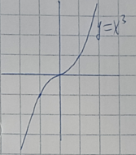
\includegraphics{4.16.1}
    \end{center}
    \underline{Замечание:} если функция непрерывна на $(a;b)$ и имеет во всех его точках, кроме, может быть \underline{конечного числа} неотрицательную (положительную) производную, то функция неубывающая (возрастающая) на $(a;b)$.

    \subsection{Необходимое и достаточное условие экстремума}
    \subsubsection*{Теорема 4.17.1}\label{th:4.17.1}
    Если $f(x)$ задана в некоторой $u(x_0)$ и точка $x_0$ - точка экстремума, тогда $f'(x_0) = 0$ или $\nexists$\par\noindent
    \underline{Доказательство:}
    \begin{adjustwidth}{1.5em}{1.5em}
        Доказательство такое же, как у \hyperref[th:4.12.1]{теоремы Ферма}.
        \begin{center}
            \textbf{Ч.т.д.}
        \end{center}
    \end{adjustwidth}
    Точки, в которых $f'(x) = 0$ будем называть \textbf{стационарными}.\\
    Если $\forall x \in u(x_0)$ $f(x) < f(x_0)$ ($f(x) > f(x_0)$), то эта точка $x_0$ - точка строгого локального максимума (минимума).
    % здесь был какой-то пример, надо будет дописать
    \subsubsection*{Теорема 4.17.2 (первое достаточное условие экстремума функции)}\label{th:4.17.2}
    %я проебал и этот моментик
    \par\noindent
    \underline{Доказательство:}
    \begin{adjustwidth}{1.5em}{1.5em}
        %да и этот
    \end{adjustwidth}
    \subsubsection*{Теорема 4.17.3 (второе достаточное условие экстремума функции)}\label{th:4.17.3}
    Пусть $x_0$ - стац. точка функции $f(x)$, $f(x)$ имеет вторую непр. производную в $u(x_0)$. Тогда, если $f''(x_0) < 0$, то точка $x_0$ - точка максимума; если $f''(x_0) > 0$, то точка $x_0$ - точка минимума.\par\noindent
    \underline{Доказательство:}
    \begin{adjustwidth}{1.5em}{1.5em}
        Разложим $f(x)$ по формуле Тейлора в точке $x_0$:
        \[ f(x) = f(x_0) + \underbrace{\frac{f'(x_0)}{1!}(x-x_0)}_{= 0} + \frac{f''(x_0)}{2!}(x-x_0)^2 + o((x-x_0)^2) \]
        Пусть $f''(x_0) < 0$. Тогда $\frac{f''(x_0)}{2!}(x-x_0)^2 < 0$. Тогда
        \[ \frac{f''(x_0)}{2!}(x-x_0)^2 + o((x-x_0)^2) < 0 \]
        Следовательно
        \[ f(x) - f(x_0) < 0 \implies f(x) < f(x_0) \]
        \[ \forall x \in u(x_0)/x_0 \]
        % мб я что-то упустил опять
        Таким образом $x_0$ - точка максимума.
        Аналогично доказывается для точки минимума.
        \begin{center}
            \textbf{Ч.т.д.}
        \end{center}
    \end{adjustwidth}
    \underline{Замечание:} если $f'(x_0) = 0$ и $f''(x_0) = 0$, то точка $x_0$ может быть точкой экстремума, а может и не быть.\\
    Точка $x_0$ называется точкой возрастания функции, если $\exists u(x_0) : \forall x \in u(x_0)/x_0$ %Я ОПЯТЬ ЧТО-ТО ПРОЕБАЛ АХВАЫХВАХЫВХА
    \subsubsection*{Теорема 4.17.4}\label{th:4.17.4}
    %ну))0
    \par\noindent

    \subsection{какой-то параграф}
    % потерял начало параграфа и определение выпуклости-вогнутости
    \subsubsection*{Теорема 4.18.1}\label{th:4.18.1}
    Если $f(x)$ имеет в точке $x_0$ вторую производную и $f'(x_0) > 0$ $(< 0)$, то $f(x)$ вогнута (выпукла) в точке $x_0$.\par\noindent
    \underline{Доказательство:}
    \begin{adjustwidth}{1.5em}{1.5em}
        Разложим $f(x)$ по формуле Тейлора в окрестности точки $x_0$.
        \[ f(x) = f(x_0) + f'(x_0)(x-x_0) + \frac{f''(\xi)}{2!}(x-x_0)^2 \]
        Уравнение касательной в точке $x_0$:
        \[ y = f(x_0) + f'(x_0)(x-x_0) \]
        Рассмотрим разность $f(x) - y$ (оценивает превышение функции над касательной)
        \[ f(x) - y = \frac{f''(\xi)}{2!}(x-x_0)^2 \]
        Пусть $f''(x_0) > 0 \implies f''(\xi) > 0$ по \hyperref[th:3.3.2]{теореме о сохранении знака} $\implies f(x) - y \ge 0 \implies f(x) \ge y$.\\
        Тогда $f(x)$ вогнута в точке $x_0$ по определению.\\
        Аналогично, если $f''(x_0) < 0$, то $f(x)$ выпукла в точке $x_0$.
        \begin{center}
            \textbf{Ч.т.д.}
        \end{center}
    \end{adjustwidth}
    \textbf{Следствие:} если $f''>0$ во всех точках $(a; b)$, то $f(x)$ вогнута на $(a; b)$.\par\noindent
    Точка $x_0$ называется точкой \textbf{перегиба} кривой $y = f(x)$, если она:
    \begin{enumerate}
        \item определена в этой точке,
        \item непрерывна в этой точке, 
        \item имеет конечную или бесконечную $f'(x_0)$, 
        \item при переходе через точку $x_0$ точка кривой, имеющая абциссу $x$, переходит с одной стороны касательной на другую или слева и справа от точки $x_0$ $f(x)$ имеет разное направление выпуклости.
    \end{enumerate}

    \subsubsection*{Теорема 4.18.2 (необходимое условие точки перегиба)}\label{th:4.18.2}
    Если точка $x_0$ - точка перегиба, то $f''(x_0) = 0$\par\noindent
    \underline{Доказательство:}
    \begin{adjustwidth}{1.5em}{1.5em}
        Предположим противное. Пусть $f''(x_0) \ne 0$.
        \[ f(x) = f(x_0) + f'(x_0)(x-x_0) + \frac{f''(x_0)}{2!}(x-x_0)^2 + o((x-x_0)^2) \]
        \[ y_{\text{кас}} = f(x_0) + f'(x_0)(x-x_0) \]
        \[ f(x)-y_{\text{кас}} = \boxed{\frac{f''(x_0)}{2!}(x-x_0)^2} + o((x-x_0)^2) \]
        Знак $f(x) - y_{\text{кас}}$ зависит от знака $f''(x_0)$.\\
        Пусть $f''(x_0) > 0 \implies \exists u(x_0) : \forall x \in u(x_0) \implies f''(x) > 0$ по \hyperref[th:3.3.2]{теореме о сохранении знака}.\\
        А это значит, что $f(x) - y_{\text{кас}} \ge 0$ $\forall x \in u(x_0) \implies x_0$ - не точка перегиба.\\
        Получили противоречие с тем, что $x_0$ - точка перегиба.
        \begin{center}
            \textbf{Ч.т.д.}
        \end{center}
    \end{adjustwidth}

    \subsubsection*{Теорема 4.18.3 (первое достаточное условие точки перегиба)}\label{th:4.18.3}
    Если $f(x)$ определена и непрерывна в точке $x_0$, имеет конечную или бесконечную производную в этой точке и при переходе через точку $x_0$ $f''(x)$ меняет знак, то точка $x_0$ - точка перегиба функции $f(x)$.\par\noindent
    \underline{Доказательство:}
    \begin{adjustwidth}{1.5em}{1.5em}
        %успешно проебал
    \end{adjustwidth}
    
    \subsubsection*{Теорема 4.18.4 (второе достаточное условие точки перегиба)}\label{th:4.18.4}
    Если $f(x)$ определена и непрерывна в точке $x_0$, $f'(x_0)$ конечна или бесконечна, $f'''$ непрерывна в точке $x_0$, $f''(x_0) = 0, f'''(x_0) \ne 0 \implies x_0$ - точка перегиба функции $f(x)$.\par\noindent
    \underline{Доказательство:}
    \begin{adjustwidth}{1.5em}{1.5em}
        \[ f(x) = f(x_0) + f'(x_0)(x-x_0) + \frac{f'''(\xi)}{3!}(x-x_0)^3 \]
        \[ y_{\text{кас}} = f(x_0) + f'(x_0)(x-X_0) \]
        \[ f(x) - y_{\text{кас}} = \boxed{ \frac{f'''(\xi)}{3!}(x-x_0)^3 } \]
        $f'''(x_0) \ne 0 \implies f'''(x)$ сохраняет знак в некоторой окрестности $x_0$\\
        При переходе через точку $x_0$ $f'''(\xi)$ знак не меняет, а $(х - х_0)^3$ меняет знак $\implies f(x) - y_{\text{кас}}$ меняет знак $\implies x_0$ - точка перегиба.
        \begin{center}
            \textbf{Ч.т.д.}
        \end{center}
    \end{adjustwidth}

    \subsubsection*{Теорема 4.18.5}\label{th:4.18.5}
    Пусть $f(x)$ определена и непрерывна в точке $x_0$, $f'(x_0)$ конечна или бесконечна,
    \[ f''(x_0) = f'''(x_0) = \dots = f^{(n)}(x_0) = 0, f^{(n+1)}(x_0) \ne 0 \]
    при $f^{(n+1)}(x)$ непрерывной в точке $x_0$, тогда \begin{itemize}
        \item если $n$ - нечётное, то в точке $x_0$ перегиба нет и функция вогнута или выпукла в точке $x_0$ в зависимости от знака $f^{(n+1)}(x_0)$,
        \item если $n$ - чётное, то $x_0$ - точка перегиба функции $f(x)$.
    \end{itemize}
    \underline{Доказательство:}
    \begin{adjustwidth}{1.5em}{1.5em}
        \[ f(x) = f(x_0) + f'(x_0)(x-x_0) + \frac{f^{(n+1)}(\xi)}{(n+1)!}(x-x_0)^{n+1} \]
        \[ y_{\text{кас}} = f(x_0) + f'(x_0)(x-x_0) \]
        \[ f(x) - y_{\text{кас}} = \frac{f^{(n+1)}(\xi)}{(n+1)!}(x-x_0)^{n+1} \]
        \begin{itemize}
            \item $n$ - чётное $\implies$ при переходе через точку $x_0$ знак $f(x) - y_{\text{кас}}$ меняется $\implies x_0$ - точка перегиба.
            \item $n$ - нечётное $\implies f(x) - y_{\text{кас}}$ не меняет знак при переходе через точку $x_0 \implies x_0$ - не точка перегиба.
        \end{itemize}
        \begin{center}
            \textbf{Ч.т.д.}
        \end{center}
    \end{adjustwidth}
    
    \subsection{Асимптоты графиков функции}
    \noindent Прямая $x = a$ называется \textbf{вертикальной асимптотой} графика функции $y = f(x)$, если хотя бы один из пределов $\lim_{x\to a-0} f(x)$ или $\lim_{x\to a + 0} f(x)$ равен $\pm \infty$.\par\noindent
    Если функция задана для $x > a$ ($x < a$) и $\exists$ такая прямая $y = kx+b$ такая, что $\lim_{x \to \infty} [ f(x) - (kx+b) ] = 0$ ($x \to -\infty$), то эта прямая называется \textbf{наклонной асимптотой} графика функции $f(x)$ при $x \to \infty$ ($x \to -\infty$).
    
    \subsubsection*{Теорема 4.19.1}\label{th:4.19.1}
    Для того, чтобы график функции $y = f(x)$ имел при $x \to \infty$ ($x \to -\infty)$ накл. асимптоту $\Leftrightarrow$ чтобы $\exists$-ли \underline{конечные} пределы
    \[ \lim_{\underset{(x \to -\infty)}{x\to +\infty}} \frac{f(x)}{x} = k; \lim_{\underset{(x \to -\infty)}{x\to +\infty}} (f(x) - kx) = b \]
    \underline{Доказательство:}
    \begin{adjustwidth}{1.5em}{1.5em}
        \textbf{Докажем необходимость ($\Rightarrow$)}\par\noindent
        Пусть $f(x)$ имеет конечную асимптоту при $x \to +\infty$.\\
        Тогда по определению
        \[ \lim_{x\to +\infty} [ f(x) - (kx+b) ] = 0 \]
        Тогда
        \[ f(x) - (kx+b) = 0 + \alpha(x); \lim_{x \to +\infty} \alpha(x) = 0 \]
        \[ \lim_{x \to +\infty}\frac{f(x)}{x} = \lim_{x\to +\infty} (k + \frac{b}{x} + \frac{\alpha(x)}{x}) = k \]
        \[ \lim_{x \to +\infty} (f(x) - kx) = \lim_{x \to +\infty}(b + \alpha(x)) = b \]
        \textbf{Докажем достаточность ($\Leftarrow$)}\par\noindent
        Пусть $\lim_{x\to +\infty} (f(x) - kx) = b$, тогда 
        \[f(x) - kx = b + \alpha(x)\]
        \[f(x) - kx - b = \alpha(x)\]
        \[ \lim_{x\to +\infty} (f(x) - (kx+b)) = 0 \]
        Т.е. $y = kx+b$ - накл. асимптота при $x \to +\infty$.

        \begin{center}
            \textbf{Ч.т.д.}
        \end{center}
    \end{adjustwidth}
    
    % -----------------------------------
    %
    %  КОНЕЦ ПЕРВОГО СЕМЕСТРА
    %
    % -----------------------------------

    
    \section{Неопределённые интегралы}
    \subsection{Определение. Основные понятия}
    \underline{Задача}. Известна производная функции $f(x)$. Требуется найти саму функцию $f(x)$.\\
    Или: по известной скорости восстановить закон движения.\par\noindent
    Функция $F(x)$ называется первообразной для функции $f(x)$ на некотором интервале $(a; b)$, если $F(x)$ дифференциуема на $(a; b)$ и $F'(x) = f(x)$.
    \subsubsection*{Теорема 5.1.1}\label{th:5.1.1}
    Если $F(x)$ первообразная для $f(x)$ на $(a; b)$, то $F(x) + \mathbb{C}$, $C = const$, тоже первообразная.\par\noindent
    \underline{Доказательство:}
    \[ (F(x) + \mathbb{C})' = F'(x) = f(x) \]
    \begin{center}
        \textbf{Ч.т.д.}
    \end{center}
    \subsubsection*{Теорема 5.1.2}\label{th:5.1.2}
    Для того, чтобы две дифференциуемые на $(a;b)$ функции были первообразными для одной и той же функции $\Leftrightarrow$ чтобы на $(a; b)$ они отличались на постоянную.\par\noindent
    \underline{Доказательство:}
    \begin{adjustwidth}{1.5em}{1.5em}
        \textbf{Докажем необходимость ($\Rightarrow$)}\par\noindent
        Пусть $F_1(x)$ и $F_2(x)$ - две первообразные для $f(x)$ на $(a; b)$.\\
        Тогда по определению $F_1'(x) = F_2'(x) = f(x)$.\\
        Пусть $\varphi(x) = F_1(x) - F_2(x), \phi'(x) = F_1'(x) - F_2'(x) = f(x) - f(x) = 0$.\\
        Тогда по \hyperref[th:4.12.5]{теореме 4.12.5} $\varphi(x) = const$.\par\noindent
        
        \textbf{Докажем достаточность ($\Leftarrow$)}\par\noindent
        Пусть
        \begin{gather*}
            F_1(x) - F_2(x) = const\\
            F_1(x) = C + F_2(x)\\
            F_1'(x) = (C + F_2(x))'\\
            f(x) = f(x)
        \end{gather*}
        \begin{center}
            \textbf{Ч.т.д.}
        \end{center}
    \end{adjustwidth}
    Совокупность всех первообразующих функции $f(x)$ на $(a; b)$ называется \underline{неопределенным интегралом} от функции $f(x)$ и обозначается 
    \[ \int f(x)dx \]
    $\int$ - знак интеграла, $f(x)dx$ - подынтегральное выражение, $f(x)$ - подынтегральная функция; $dx$ - знак.
    
    \subsection{Свойства неопределённого интеграла}
    \begin{enumerate}
        \item \[ d \int f(x) dx = f(x)dx \]
        \underline{Доказательство:}
        \[ d \int f(x)dx = d(F(x) + \mathbb{C}) = (F(x) + \mathbb{C})'dx = f(x)dx \]
        \begin{center}
            \textbf{Ч.т.д.}
        \end{center}
        \item \[ \int dF(x) = F(x) + \mathbb{C} \]
        \underline{Доказательство:}
        \[ \int dF(x) = \int F'(x)dx = \int f(x)dx = F(x) + \mathbb{C} \]
        \begin{center}
            \textbf{Ч.т.д.}
        \end{center}
        \item \[ \int k f(x) dx = k \int f(x) dx, k = const \]
        \underline{Доказательство:}
        \begin{adjustwidth}{1.5em}{1.5em}
            $F'(x) = f(x)$\\
            $(k(F(x)))' = kf(x)$, т.е. $kF(x)$ является первообразной для $kf(x)$ на $(a; b)$\\
            Т.е. левая часть: $\int kf(x)dx = kF(x) + \mathbb{C}_1$\\
            А правая часть: $k \int f(x)dx = k(F(x) + \mathbb{C}_2) = kF(x) + kC_2$, если обозначать $C_1 = kC_2$, то \textbf{ч.т.д.}
        \end{adjustwidth}
        \item \[ \int (f(x) \pm g(x)) dx = \int f(x) dx \pm \int g(x)dx \]
        \underline{Доказательство:}
        \begin{adjustwidth}{1.5em}{1.5em}
            Докажем для "+"\par\noindent
            По определению: $F_1'(x) = f(x)$, $F_2'(x) = g(x)$\\
            $(F_1 + F_2)' = F_1' + F_2' = f(x) + g(x)$\\
            Т.е. по определению $F_1(x) + F_2(x)$ является первообразной для функции $f(x) + g(x)$\\
            левая часть: $\int (f(x) + g(x))dx = F_1(x) + F_2(x) + \mathbb{C}_1$\\
            правая часть: $\int f(x)dx + \int g(x)dx = F_1(x) + \mathbb{C}_2 + F_2(x) + \mathbb{C}_3$\\
            Если обозначать $C_1 = kC_2$, то \textbf{ч.т.д.}
        \end{adjustwidth}
        \item \[ \int (k_1 f(x) + k_2 g(x))dx = k_1 \int f(x)dx + k_2 \int g(x)dx \]
        \underline{Доказательство:}
        \begin{adjustwidth}{1.5em}{1.5em}
            По определению: $F_1'(x) = f(x), F_2'(x) = g(x)$\\
            $(k_1F_1(x) + k_2F_2(x))' = k_1f(x) + k_2g(x)$, т.е. по определению $(k_1F_1(x) + k_2F_2(x))$ является первообразной для функции $k_1f(x) + k_2g(x)$ на $(a; b)$\\
            Т.е. левая часть: $\int (k_1f(x) + k_2g(x))dx = k_1F_1(x) + k_2F_2(x) + \mathbb{C}_1$\\
            правая часть: $k_1\int f(x)dx + k_2\int g(x)dx = k_1(F_1(x) + \mathbb{C}_2) + k_2(F_2(x) + \mathbb{C}_3) = k_1F_1(x) + k_1\mathbb{C}_2 + k_2F_2(x) + k_2\mathbb{C}_3$\\
            Если обозначать $\mathbb{C}_1 = k_1\mathbb{C}_2 + k_2\mathbb{C}_3$, то \textbf{ч.т.д.}
        \end{adjustwidth}
    \end{enumerate}

    \subsection{Формула замены переменной в неопределённом интеграле}
    \subsubsection*{Теорема 5.3.1}\label{th:5.3.1}
    Пусть функции $y=f(x)$ и $x=\varphi(t)$ определены на $\Delta x$ и $\Delta t$ и $\varphi(\Delta t) \subset \Delta x$.\\
    Если $f(x)$ имеет на $\Delta x$ первообразную $F(x)$, т.е. $\int \,f(x)dx = F(x) + \mathbb{C}$, а $\varphi(t)$ дифференциуема на $\Delta t$, то функция $F(\varphi(t))\phi'(t)$ имеет на $\Delta t$ первообразная $F(\varphi(t))$
    \[ \boxed{\int \, f(x)dx = \int f(\varphi(t))\phi'(t)dt} \]
    \underline{Доказательство:}
    \begin{adjustwidth}{1.5em}{1.5em}
        Функции $f(x)$ и $F(x)$ определены на $\Delta x$, $\phi (\Delta t)$ с $\Delta x$, т.е. определены сложные функции\\
        $f(\varphi(t))$ и $F(\varphi(t))$
        \[ F(\varphi(t))' = F'(\varphi(t)) * \phi'(t) = f(\varphi(t)) * \phi'(t) \]
        Т.е. по определению функция $F(\varphi(t))$ является первообразной для $f(\varphi(t))\phi'(t)$\\
        Тогда $\underbrace{ f(\varphi(t))\phi'(t)dt } = F(\varphi(t)) + \mathbb{C} = F(x) + \mathbb{C} = \underbrace{ \int f(x)dx }$
        \begin{center}
            \textbf{Ч.т.д.}
        \end{center}
    \end{adjustwidth}
    \underline{Примеры:}
    \begin{enumerate}
        \item \begin{gather*}
            \int \tg(x)dx = \int \frac{\sin x dx}{\cos x} = \begin{vmatrix}
                t = \cos x\\
                x = \arccos t\\
                dx = - \frac{1}{\sqrt{1 - t^2}}dt
            \end{vmatrix} = - \int \frac{\sqrt{1 - t^2}dt}{\sqrt{1 - t^2}t} = - \int \frac{dt}{t} =\\
            = -\ln |t| + \mathbb{C} = -\ln |\cos x| + \mathbb{C}
        \end{gather*}
        \item \begin{gather*}
            \int \sqrt{1 - x^2}dx = \begin{vmatrix}
                x = \sin t\\
                dx = \cos t dt
            \end{vmatrix} = \int \sqrt{1 - \sin^2 t}\cos t dt = \int \cos^2 t dt =\\
            = \int \frac{1+\cos 2t}{2}dt = \int \frac{1}{2}dt + \int \frac{\cos 2t}{2}dt = \frac{1}{2}t + \frac{1}{4}\sin 2t + \mathbb{C} = \frac{1}{2}\arcsin x + \frac{1}{4}\sin (2\arcsin x) + \mathbb{C}
        \end{gather*}
    \end{enumerate}

    \subsubsection*{Таблица интегралов}
    % я не буду это писать
    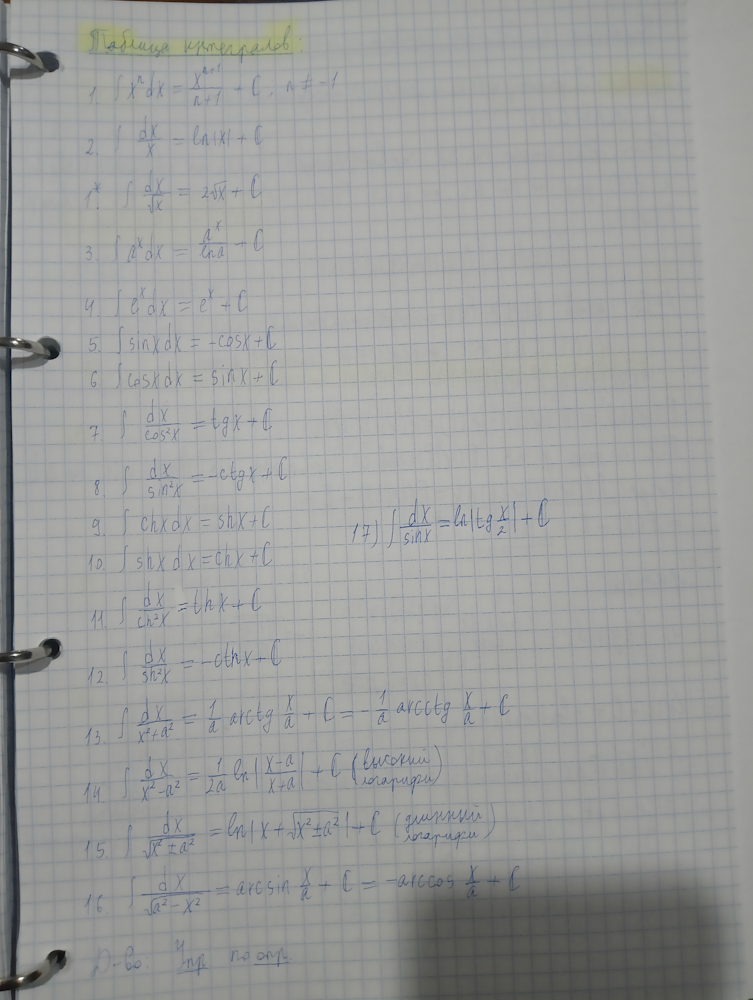
\includegraphics[width=0.7\linewidth,keepaspectratio]{5.3.1.png}

    \subsection{Формула интегрирования по частям}
    \subsubsection*{Теорема 5.4.1}\label{th:5.4.1}
    Если функции $u(x)$ и $v(x)$ дифференциуемы на некотором промежутке и на этом промежутке $\exists \int vdu$, то на нём $\exists \int udv$ и
    \[ \boxed{\int udv = uv - \int vdu} \]
    \underline{Доказательство:}
    \begin{adjustwidth}{1.5em}{1.5em}
        \begin{gather*}
            \int udv = \int uv'dx = \left| (uv)' = u'v + uv' \right| =\\
            = \int [(uv)' - u'v]dx = \int (uv)'dx - \int u'vdx = uv - \int vdu
        \end{gather*}
        \begin{center}
            \textbf{Ч.т.д.}
        \end{center}
    \end{adjustwidth}

    \subsubsection*{Формула интегрирования по частям применяется в случаях:}    
    \begin{enumerate}
        \item \begin{gather*}
            \int P_n(x) * \underset{\text{таблич. интегралы}}{\begin{Bmatrix}
                \sin \alpha x\\
                \cos \alpha x\\
                e^{\alpha x}\\
                \dots
            \end{Bmatrix}}dx,\, \begin{matrix}
                u = P_n(x) & du = \dots \\
                dv = \underset{\text{табл}}{\left\{ \dots \right\}}dx & v = \dots
            \end{matrix}
        \end{gather*}
        \item \begin{gather*}
            \int P_n(x) * \underset{\text{не таблич.}}{\begin{Bmatrix}
                \arcsin \alpha x\\
                \arctg \alpha x\\
                ln \alpha x\\
                \dots
            \end{Bmatrix}}dx,\,\begin{matrix}
                u = \left\{ \dots \right\} & du = \dots \\
                dv = P_n(x)dx & v = \dots
            \end{matrix}
        \end{gather*}
        \item \begin{gather*}
            \int \underset{\text{не таблич.}}{\begin{Bmatrix}
                \arcsin \alpha x\\
                \arctg \alpha x\\
                ln \alpha x\\
                \dots
            \end{Bmatrix}}dx,\,\begin{matrix}
                u = \left\{ \dots \right\} & du = \dots \\
                dv = dx & v = x
            \end{matrix}
        \end{gather*}
        % \item \begin{gather*} 
        %     = \int \frac{(Bx + \mathbb{C})dx}{(x+\frac{p}{2})^2 + a^2} = \begin{vmatrix}
        %         x + \frac{p}{2} = t\\
        %         x = t - \frac{p}{2}\\
        %         dx = dt
        %     \end{vmatrix} = \int \frac{(B(t-\frac{p}{2})+C)dt}{t^2 + a^2} = B \int \frac{tdt}{t^2+a^2} + (-\frac{Bp}{2} + \mathbb{C}) \int \frac{dt}{t^2+a^2} =\\
        %     = \frac{B}{2}\ln|t^2+a^2| + \frac{1}{a}\left(-\frac{Bp}{2} + \mathbb{C}\right)\arctg \frac{t}{a} + \mathbb{C}
        % \end{gather*}
        % \item \begin{gather*}
        %     \int \frac{(Ax+B)}{(x^2 + px + q)^k}dx = \int \frac{(Ax+B)}{(x^2 + \boxed{2} * \frac{1}{2}p\boxed{x} + \frac{p^2}{4} - \frac{p^2}{4} + q)^k}dx =\\
        %     = \int \frac{(Ax+B)dx}{[(x + \frac{p}{2})^2 + \underbrace{q - \frac{p^2}{4}}_{a^2, \, >0}]^k} = \begin{vmatrix}
        %         t = x + \frac{p}{2}\\
        %         x = t - \frac{p}{2}\\
        %         dx = dt
        %     \end{vmatrix} = \int \frac{A(t - \frac{p}{2}) + B}{(t^2 + a^2)^k}dt =\\
        %     = A \int \frac{tdt}{(t^2 + a^2)^k} + \left(-\frac{Ap}{2} + B\right)\int \frac{dt}{(t^2 + a^2)^k} = \frac{A}{2}
        % \end{gather*}
    \end{enumerate}
    \underline{Примеры:}
    \begin{enumerate}
        \item \[ \int \ln x dx = \begin{vmatrix}
            u = \ln x & du = \frac{dx}{x} \\
            dv = dx & v = x
        \end{vmatrix} = x\ln x - \int dx = x\ln x - x + \mathbb{C} \]
        \item \[ \int x \sin x dx = \begin{vmatrix}
            u = x & du = dx\\
            dv = \sin x dx & v = -\cos x
        \end{vmatrix} = -x \cos x + \int \cos x dx = -x \cos x + \sin x + \mathbb{C} \]
    \end{enumerate}

    \subsection{Интегрирование рациональных дробей}
    \subsubsection*{Элементарные дроби}
    \begin{enumerate}
        \item \[\frac{A}{x-a}\]
        \item \[\frac{A}{(x-a)^k}\]
        \item \[\frac{Bx+C}{x^2+px+q}\]
        \item \[\frac{Bx+C}{(x^2+px+q)^k}\]
    \end{enumerate}
    Покажем, что элементарные дроби интегрируются:
    \begin{enumerate}
        \item \[ \int \frac{A}{x - a}dx = A\int \frac{d(x-a)}{x-a} = A\ln|x-a| + \mathbb{C} \]
        \item \[ \int \frac{A}{(x - a)^k}dx = A\int (x-a)^{-k} \frac{d(x-a)}{x-a} = A \frac{(x-a)^{-k+1}}{-k+1} + \mathbb{C} \]
        \item \begin{gather*} 
            \int \frac{(Bx+C)}{x^2+px+q}dx = \int \frac{(Bx+C)dx}{x^2+2*\frac{1}{2}px + \frac{p^2}{4} - \frac{p^2}{4} + q} =\\
            = \int \frac{(Bx+C)dx}{(x+\frac{p}{2})^2 + \underset{a^2}{\underbrace{q - \frac{p^2}{4}}}} = \int \frac{(Bx+C)dx}{(x+\frac{p}{2})^2+a^2} =\\
            = \begin{vmatrix}
                t = x + \frac{p}{2}\\
                x = t - \frac{p}{2}\\
                dx = dt
            \end{vmatrix} = \int \frac{(B(t - \frac{p}{2}) + C)dt}{t^2 + a^2} = B \int \frac{tdt}{t^2+a^2} + (-\frac{Bp}{2} + \mathbb{C})\int \frac{dt}{t^2+a^2} =\\
            = \frac{B}{2}\ln|t^2+a^2| + \frac{1}{a}(-\frac{Bp}{2} + \mathbb{C})\arctg \frac{t}{a} + \mathbb{C} = \left|t = x+\frac{p}{2}\right| =\\
            = \frac{B}{2}\ln\left|(x + \frac{p}{x})^2 + a^2\right| + \frac{1}{a}(-\frac{Bp}{2} + \mathbb{C})\arctg \frac{x+2}{a} + \mathbb{C}
        \end{gather*}
        \item \begin{gather*}
            \int \frac{Ax+B}{(x^2 + px + q)^k}dx = \int \frac{(Ax+B)dx}{(x^2+2*\frac{1}{2}px + \frac{p^2}{4} - \frac{p^2}{4} + q)^k} = \int \frac{(Ax+B)dx}{[(x+\frac{p}{2})^2 + \underset{a^2}{\underbrace{q - \frac{p^2}{4}}}]^k} =\\
            = \begin{vmatrix}
                t = x + \frac{p}{2}\\
                x = t - \frac{p}{2}\\
                dx = dt
            \end{vmatrix} = \int \frac{A(t - \frac{p}{2}) + B}{(t^2 + a^2)^k}dt = A \int \frac{tdt}{(t^2 + a^2)^k} + (-\frac{Ap}{2} + B)\int \frac{dt}{(t^2 + a^2)^k} =\\
            = \frac{A}{2}\frac{(t^2 + a^2)^{-k+1}}{-k+1} + (-\frac{Ap}{2} + B)\int \frac{dt}{(t^2 + a^2)^k}
        \end{gather*}
        Рассмотрим
        \begin{gather*}
            I_k = \int \frac{1dt}{(t^2 + a^2)^k} = \frac{1}{a^2} \int \frac{(t^2 + a^2 - t^2)dt}{(t^2 + a^2)^k} = \frac{1}{a^2} \int \frac{dt}{(t^2+a^2)^{k-1}} - \frac{1}{a^2}\int\frac{t^2dt}{(t^2 + a^2)^k} =\\
            = \frac{1}{a^2}I_{k-1} - \begin{vmatrix}
                u = t & du = dt\\
                dv = \frac{tdt}{(t^2 + a^2)^k} & v = \frac{1}{2}\frac{(t^2+a^2)^{-k+1}}{(1-k)}\\
            \end{vmatrix} =\\
            = \frac{1}{a^2}I_{k-1} - \frac{1}{a^2} \left( \frac{t}{2(1-k)(t^2+a^2)^{k-1}} - \frac{1}{2(1-k)} \right) \int \frac{dt}{(t^2 + a^2)^{k-1}} =\\
            = \frac{1}{a^2}I_{k-1} + \frac{t}{2a^2(k-1)(t^2+a^2)^{k-1}} - \frac{1}{2a^2(k-1)}I_{k-1} =\\
            = \left| \frac{1}{a^2}(1 - \frac{1}{2(k-1)}) = \frac{1}{a^2}\frac{(2k-3)}{2(k-1)} \right| =\\
            = \frac{t}{2a^2(k-1)(t^2+a^2)^{k-1}} + \frac{2k-3}{a^2(2k-2)}I_{k-1}
        \end{gather*}
    \end{enumerate}
    \underline{Пример:}
    \begin{gather*}
        \int \frac{7x^2 + 26x - 9}{x^4 + 4x^3 + 4x^2 - 9}dx = \int \frac{7x^2 + 26x - 9}{(x-1)(x+3)(x^2 + 2x + 3)dx} \boxed{=}
    \end{gather*}
    \begin{gather*}
        \frac{7x^2 + 26x - 9}{(x-1)(x+3)(x^2+2x+3)} = \frac{A}{x-1} + \frac{B}{x+3} + \frac{Cx+D}{x^2+2x+3} =\\
        = \frac{A(x+3)(x^2+2x+3) + B(x-1)(x^2+2x+3) + (Cx+D)(x-1)(x+3)}{(x-1)(x+3)(x^2+2x+3)2C}
    \end{gather*}
    \begin{align*}
        &x^3 : & 0 &= A+B+C\\
        &x^2 : & 7 &= 5A+B+2C+D\\
        &x^1 : & 26 &= 9A+B-3C+2D\\
        &x^0 : & -9 &= 9A-3B-3D
    \end{align*}
    \begin{gather*}
        A = 1, B = 1, C = -2, D = 5
    \end{gather*}
    \begin{gather*}
        \boxed{=} \int \frac{dx}{x-1} + \int \frac{dx}{x+3} + \int \frac{-2x+5}{x^2+2x+3}dx =\\
        = \int \frac{dx}{x-1} + \int \frac{dx}{x+3} + (-1) \int \frac{2x+2 - 2 - 1*5}{x^2+2x+3}dx =\\
        = \int \frac{dx}{x-1} + \int \frac{dx}{x+3} - \int \frac{2x+2}{x^2+2x+3}dx + 7\int \frac{d(x+1)}{(x+1)^2+2} =\\
        = \int \frac{dx}{x-1} + \int \frac{dx}{x+3} - \int \frac{d(x^2+2x+3)}{x^2+2x+3}dx + 7\int \frac{d(x+1)}{(x+1)^2+2} =\\
        = \ln |x-1| + \ln |x+3| - \ln |x^2+2x+3| + \frac{7}{\sqrt{2}}\arctg \frac{x+1}{\sqrt{2}} + \mathbb{C}
    \end{gather*}

    \subsection{Интегрирование тригонометрических функций}
    \begin{enumerate}
        \item $\int \cos^{2n+1}x dx; \int \sin^{2n+1}x dx$\\
        \underline{Замены:} используем метод подстановки: $t = \sin x$ и $t = \cos x$ соответственно.
        \item $\int \cos^{2n}x dx; \int \sin^{2n}x dx$\\
        \underline{Замены:} используем тригонометрические формулы уменьшения степени:
        \[ \cos^{2}x = \frac{1+\cos 2x}{2}; \sin^2x = \frac{1-\cos 2x}{2} \]
        \underline{Замечание:} аналогично решаются примеры вида $\int \sin^{2n}x \cos^{2n}x dx$
        \item $\int \sin mx \cos nx dx; \int \sin mx \sin nx dx; \int \cos mx \cos nx dx$\\
        \underline{Замены:} используем тригонометрические формулы:
        \begin{gather*}
            \sin mx \cos nx = \frac{1}{2}\left[ \sin(m-n)x + \sin(m+n)x \right]\\
            \sin mx \sin nx = \frac{1}{2}\left[ \cos(m-n)x - \cos(m+n)x \right]\\
            \cos mx \cos nx = \frac{1}{2}\left[ \cos(m-n)x + \cos(m+n)x \right]
        \end{gather*}
        \item $\int \tg^nx dx; \int \ctg^nx dx$\\
        \underline{Замены:} 
        \[ \boxed{ \tg^2x = \frac{1}{\cos^2x}-1; \ctg^2x = \frac{1}{\sin^2x}-1 } \]
        \item Интегралы вида $\int R(\sin x; \cos x)dx$\\
        \subsubsection*{Универсальная тригонометрическая подстановка}
        \[ \boxed{t = \tg \frac{x}{2}} \]
        \[ \boxed{\sin x = \frac{2\tg\frac{x}{2}}{1 + \tg^2 \frac{x}{2}} = \frac{2t}{1 + t^2}} \]
        \[ \boxed{\cos x = \frac{1-t^2}{1 + t^2}} \]
        \[ \frac{x}{2} = \arctg t, \,\,\, x = 2 \arctg t, \,\,\, \boxed{ dx = \frac{2dt}{1+t^2}} \text{ - ВЫУЧИТЬ!} \]
        Интеграл от дробно-рациональной функции:
        \[ \int R(\sin x; \cos x)dx = \int R\left( \frac{2t}{1+t^2}\frac{1-t^2}{1+t^2} \right)\frac{2dt}{1+t^2} \]
        \underline{Примеры:}
        \begin{enumerate}
            \item \begin{gather*} 
                \int \frac{dx}{3 + 5\cos x} = \begin{vmatrix}
                    t = \tg \frac{x}{2}\\
                    \cos x = \frac{1 - t^2}{1 + t^2}\\
                    dx = \frac{2dt}{1 + t^2}
                \end{vmatrix} = \int \frac{\frac{2dt}{1+t^2}}{3 + \frac{5-5t^2}{1 + t^2}} = \int \frac{\frac{2dt}{1 + t^2}}{\frac{3 + 3t^2 + 5 - 5t^2}{1 + t^2}} =\\
                = 2 \int \frac{dt}{-2t^2 + 8} = - \int \frac{dt}{t^2 - 4} = -\frac{1}{4} \ln \left|\frac{t-2}{t+2}\right| + \mathbb{C} = -\frac{1}{4}\ln \left|\frac{\tg\frac{x}{2} - 2}{\tg\frac{x}{2} + 2}\right| + \mathbb{C}
            \end{gather*}
            \item \begin{gather*}
                \int \frac{dx}{\sin x} = \begin{vmatrix}
                    t = \tg \frac{x}{2}\\
                    \sin x = \frac{2t}{1+t^2}\\
                    dx = \frac{2dt}{1+t^2}
                \end{vmatrix} = \int \frac{\frac{2dt}{1+t^2}}{\frac{2t}{1+t^2}} = \int \frac{2dt}{2t} = \ln |t| + \mathbb{C} = \ln |\tg \frac{x}{2}| + \mathbb{C}
            \end{gather*}
        \end{enumerate}
        \textbf{Частные случаи:}
        \begin{enumerate}
            \item Подынтегральная функция нечётна относительно $\sin x$.
            \[ \int R (-\sin x; \cos x)dx = - \int R(\sin x; \cos x)dx \]
            \underline{Пример:} $\frac{\sin^3x}{\cos^4x}$. \underline{Замена:} $\boxed{t = \cos x}$
            \item Подынтегральная функция нечётна относительно $\cos x$.
            \[ \int R (\sin x; -\cos x)dx = - \int R(\sin x; \cos x)dx \]
            \underline{Пример:} $\cos^5x\sin^8x$. \underline{Замена:} $\boxed{t = \sin x}$
            \item Подынтегральная функция чётна или нечётна относительно обоих $\sin x$ и $\cos x$.
            \[ \int R (-\sin x; -\cos x)dx = \int R(\sin x; \cos x)dx \]
            \underline{Пример:} $\sin^2x \cos^6x$ или $\sin^3x \cos^5x$. \underline{Замены:}
            \[ t = \tg x \] 
            \[\boxed{\sin x = \frac{\tg x}{\sqrt{1 + \tg^2 x}} = \frac{t}{\sqrt{1 + t^2}}} \]
            \[ \boxed{\cos x = \frac{1}{\sqrt{1 + t^2}}} \]
            \[ x = \arctg t \]
            \[ \boxed{dx = \frac{dt}{1+t^2}} \text{ - ВЫУЧИТЬ!} \]
        \end{enumerate}
        \underline{Примеры:}
        \begin{enumerate}
            \item \begin{gather*}
                \int \frac{\sin^3 xdx}{\cos^4 x} = \begin{vmatrix}
                    t = \cos x
                \end{vmatrix} = - \int \frac{\sin^2x d\cos x}{\cos^4 x} = - \int \frac{(1 - \cos^2x)d\cos x}{\cos^4 x} =\\
                = -\int\frac{d\cos x}{\cos^4 x} - \int \frac{\cos^2 x d\cos x}{\cos^4 x} = \frac{1}{3\cos^3 x} - \frac{1}{\cos x} + \mathbb{C}
            \end{gather*}
            \item \begin{gather*}
                \int \frac{dx}{4\cos^2x + 3\sin^2x} = \begin{vmatrix}
                    t = \tg x\\
                    \sin x = \frac{t}{\sqrt{1 + t^2}}\\
                    \cos x = \frac{1}{\sqrt{1 + t^2}}\\
                    dx = \frac{dt}{1 + t^2}
                \end{vmatrix} = \int \frac{\frac{dt}{1+t^2}}{\frac{4}{1+t^2} + \frac{3t^2}{1 + t^2}} = \int \frac{dt}{3t^2+4} =\\
                = \frac{1}{\sqrt{3}}\int \frac{d(\sqrt{3}t)}{(\sqrt{3}t)^2 + 4} = \frac{1}{2\sqrt{3}}\arctg \frac{\sqrt{3}\tg x}{2} + \mathbb{C}
            \end{gather*}
        \end{enumerate}
    \end{enumerate}
    
    \subsection{Интегрирование иррациональных функций}
    \begin{enumerate}
        \item $\int R(x, \sqrt{a^2 - x^2})dx$\\
        \underline{Замена:} 
        \[ x = a \sin t \text{ или } x = a \cos t \]
        Замена $a \sin t$ удобнее:
        \[ \sqrt{a^2 - x^2} = \sqrt{a^2 - a^2 \sin^2 t} = \sqrt{a^2(1 - \sin^2 t)} = a \cos t \]
        \[ dx = a \cos t dt \]

        \item $\int R(x, \sqrt{x^2 + a^2})dx$\\
        \underline{Замена:} 
        \[ x = a \tg t \text{ или } x = a \ctg t \]
        Замена $a \tg t$ удобнее:
        \[ \sqrt{x^2 + a^2} = \sqrt{a^2 tg^2 t + a^2} = \frac{a}{\cos t} \]
        \[ dx = \frac{a}{\cos^2 t}dt \]

        \item $\int R(x, \sqrt{x^2 - a^2})dx$\\
        \underline{Замена:}
        \[ x = \frac{a}{\cos t} \text{ или } x = \frac{a}{\sin t} \]
        Замена $\frac{a}{\cos t}$ удобнее:
        \[ \sqrt{x^2 - a^2} = \sqrt{\frac{a^2}{\cos^2 t} - a^2} = a \tg t \]
        \[ dx = \frac{a \sin t}{\cos^2 t}dt \]
        \underline{Пример:}
        \begin{gather*}
            \int \frac{\sqrt{1 - x^2}dx}{x} = \begin{vmatrix}
                x = \sin t\\
                t = \arcsin x\\
                dx = \cos t dt
            \end{vmatrix} = \int \frac{\cos^2 t}{\sin t}dt = \int \frac{1 - \sin^2 t}{\sin t}dt = \int \frac{dt}{\sin t} - \int \sin t dt =\\
            = \ln \left| \tg \frac{t}{2} \right| + \cos t + \mathbb{C} = \ln \left| \tg \frac{\arcsin x}{2} \right| + \cos (\arcsin x) + \mathbb{C}
        \end{gather*}

        \item \[ I = \int R\left( x, \left(\frac{ax+b}{cx+d}\right)^{r_1}, \dots, \left( \frac{ax+b}{cx+d} \right)^{r_n} \right)dx \boxed{=}\]
        $r_1, \dots, r_n$ - рац. числа.
        \[ r_1 = \frac{p_1}{m},\, r_2 = \frac{p_2}{m}, \dots, r_n = \frac{p_n}{m} \]
        $m$ - общий знаменатель дробей $r$.\\
        \underline{Замена:}
        \[ \boxed{\frac{ax + b}{cx + d} = t^m} \]
        \[ x = \frac{t^m * d - b}{a - ct^m} = p(t) \]
        \[ dx = p'(t)dt \]
        \[ \boxed{=} \int R (p(t), (t^m)^{\frac{p_1}{m}}, \dots, (t^m)^{\frac{p_n}{m}})p'(t)dt = \underbrace{\int R_1(t)dt}_{\text{дробно рац. ф-ия}} \]
        \underline{Частный случай:}
        \[ I = \int R(x, (ax+b)^{r_1}, \dots, (ax+b)^{r_n})dx \to ax+b = t^m \]
        \[ I = \int R(x, x^{r_1}, \dots, x^{r_n} ) \to x = t^m \]
        \underline{Пример:}
        \begin{gather*}
            \int \frac{xdx}{\sqrt[3]{1+x} - \sqrt{1 + x}} = \begin{vmatrix}
                \frac{1}{3} : \frac{1}{2} \to 6\\
                t = \sqrt[6]{1 + x}\\
                1 + x = t^6\\
                x = t^6 - 1\\
                dx = 6t^5dt
            \end{vmatrix} = \int \frac{(t^6 - 1)6t^5dt}{t^2 - t^3} = -6 \int \frac{(t^6 - 1)t^3}{t-1}dt =\\
            = -6 \int t^3(t^5 + t^4 + t^2 + t + 1)dt = \dots \text{(дальше разбивать на сумму интегралов и всё по старому)}
        \end{gather*}

        \item Интегралы от дифференциального бинома
        \[ \int (a + bx^n)^p x^m dx \]
        \[ a,b \in R; m,n,p \in Q \]
        Интегрируются только в трёх случаях:
        \begin{enumerate}
            \item $p$ - целое. \underline{Замена:} $x = t^s$, где $s$ - общий знаменатель дробей $m$ и $n$.
            \item $p$ - дробь, $\frac{m+1}{n}$ - целое. \underline{Замена:} $a + bx^n = t^s$, где $s$ - знаменатель дроби $p$.
            \item $p$ - дробь, $\frac{m+1}{n}$ - дробь, $p + \frac{m+1}{n}$ - целое. \underline{Замена:} $ax^{-n} + b = t^s$, где $s$ - знаменатель дроби $p$.
        \end{enumerate}
        \underline{Пример:}
        \begin{gather*}
            \int \frac{\sqrt[3]{(1+2x^3)^2}dx}{x^6} = \int (1 - 2x^3)^{\frac{2}{3}}x^{-6}dx \boxed{=}\\
            p = \frac{2}{3}\, n = 3\, m = 6\\
            \boxed{=} \begin{vmatrix}
                x^{-3} + 2 = t^3\\
                -3x^{-4}dx = 3t^2dt\\
                x^{-4}dx = -t^2dt
            \end{vmatrix} = \int [x^3(x^{-3}+2)]^{\frac{2}{3}}x^{-6}dx = \int x^2(x^{-3}+2)^\frac{2}{3}x^{-6}dx = \int (x^{-3} + 2)^{\frac{2}{3}}x^{-4}dx =\\
            = \int (t^3)^\frac{2}{3} - t^2dt = -\int t^4dt = -\frac{t^5}{5} + \mathbb{C} = \begin{vmatrix}
                x^{-3} = t^3-2\\
                t^3 = x^{-3} + 2\\
                t = (x^{-3}+2)^{\frac{1}{3}}
            \end{vmatrix} = -\frac{\sqrt[3]{(x^{-3}+2)^2}(x^{-3}+2)}{5}
        \end{gather*}

        \item Интеграл вида
        \[ \int R (x, \sqrt{ax^2 + bx + c})dx \]
        \underline{\textbf{Подстановки Эйлера:}}
        \begin{enumerate}
            \item I подстановка Эйлера (при $a > 0$)
            \[ \sqrt{ax^2 + bx + c} = t \pm x\sqrt{a} \]
            \[ \cancel{ax^2} + bx + c = t^2 \pm 2tx\sqrt{a} + \cancel{ax^2} \Rightarrow x, dx \]
            \item II подстановка Эйлера (при $c > 0$)
            \[ \sqrt{ax^2 + bx + c} = tx \pm \sqrt{c} \]
            \[ ax^2 + bx + \cancel{c} = t^2x^2 \pm 2tx\sqrt{c} + \cancel{c} \]
            \[ ax+b = t^2x \pm 2t\sqrt{c} \Rightarrow x, dx \]
            \item III подстановка Эйлера (при $ax^2 + bx + c = 0 \Rightarrow \exists x_1, x_2 \in R$)
            \[ \sqrt{\frac{a(x-x_1)}{x-x_2}} = t \sqrt{ax^2 + bx + c} = \sqrt{a(x-x_1)(x-x_2)} = \sqrt{\frac{a(x-x_1)(x-x_2)^2}{x-x_2}} = t(x-x_2) \]
            \[ \frac{a(x-x_1)}{x-x_2} = t^2 \Rightarrow x, dx \]
        \end{enumerate}
        \underline{Пример:}
        \begin{gather*}
            \int \frac{dx}{x + \sqrt{x^2+x+1}} = \begin{vmatrix}
                \sqrt{x^2 + x + 1} = t - x & dx = \frac{2t(2t+1)-2(t^2-1)}{(2t+1)^2} \\
                x^2 + x + 1 = t^2 - 2tx + x^2 & dx = \frac{2t^2 + 2t + 2}{(2t+1)^2}dt\\
                x(1 + 2t) = t^2 - 1\\
                x = \frac{t^2 - 1}{2t + 1}
            \end{vmatrix} = \int \frac{2t^2 + 2t + 2}{(2t+1)^2t}dt \boxed{=}\\
            \frac{2t^2 + 2t + 2}{(2t+1)^2t} = \frac{A}{2t+1} + \frac{B}{(2t+1)^2} + \frac{C}{t} = \frac{2At^2 + At + Bt + 4t^2C + 4Ct + C}{(2t+1)^2t}\\
        \end{gather*}
        \begin{align*}
            t^2 :\, &2A + 4C = 2\\
            t^1 :\, &A + B + 4C = 2\\
            t^0 :\, &C = 2
        \end{align*}
        \begin{gather*}
            A = -3\, B = -3\, C = 2\\
            \boxed{=} \int \frac{-3dt}{2t+1} - \int \frac{3dt}{(2t+1)^2}+2 \int \frac{dt}{t} = -3 \int \frac{dt}{2t+1} - 3 \int \frac{dt}{(2t+1)^2} + 2 \int \frac{dt}{t} =\\
            = -\frac{3}{2}\int \frac{d(2t+1)}{2t+1} - \frac{3}{2}\int \frac{d(2t+1)}{(2t+1)^2} + 2\int\frac{dt}{t} = -\frac{3}{2}\ln |2t+1| + \frac{3}{2}\frac{1}{2t+1} + 2 \ln |t| + \mathbb{C} =\\
            = -\frac{3}{2} \ln |2\sqrt{x^2+x+1}+2x+1| + \frac{3}{2}\frac{1}{2\sqrt{x^2+x+1}+2x+1} + 2 \ln |\sqrt{x^2+x+1}+x| + \mathbb{C}
        \end{gather*}

        \item Интегралы вида
        \[ \int \frac{dx}{(x-\alpha)\sqrt{ax^2 + bx + c}} \]
        \underline{Замена:} 
        \[ \boxed{t = \frac{1}{x-\alpha}} \]
        \underline{Пример:}
        \[ \int \frac{dx}{(x-1)\sqrt{-x^2+3x-2}} = \begin{vmatrix}
            t = \frac{1}{x-1}\\
            x - 1 = \frac{1}{t}\\
            x = \frac{1}{t} + 1\\
            dx = -\frac{1}{t^2}dt
        \end{vmatrix} = \int \frac{-\frac{1}{t^2}dt}{\frac{1}{t}\sqrt{-\left( \frac{1}{t} + 1 \right)^2 + \frac{3}{t} + 3 - 2}} \]
    \end{enumerate}

    \section{Определенный интеграл. Геометрические и физические приложения определенного интеграла. Несобственные интегралы}
    \subsection{Задачи приводящие к понятию определённого интеграла.}
    \subsection*{1. Площадь криволинейной трапеции} 
    \begin{center}
        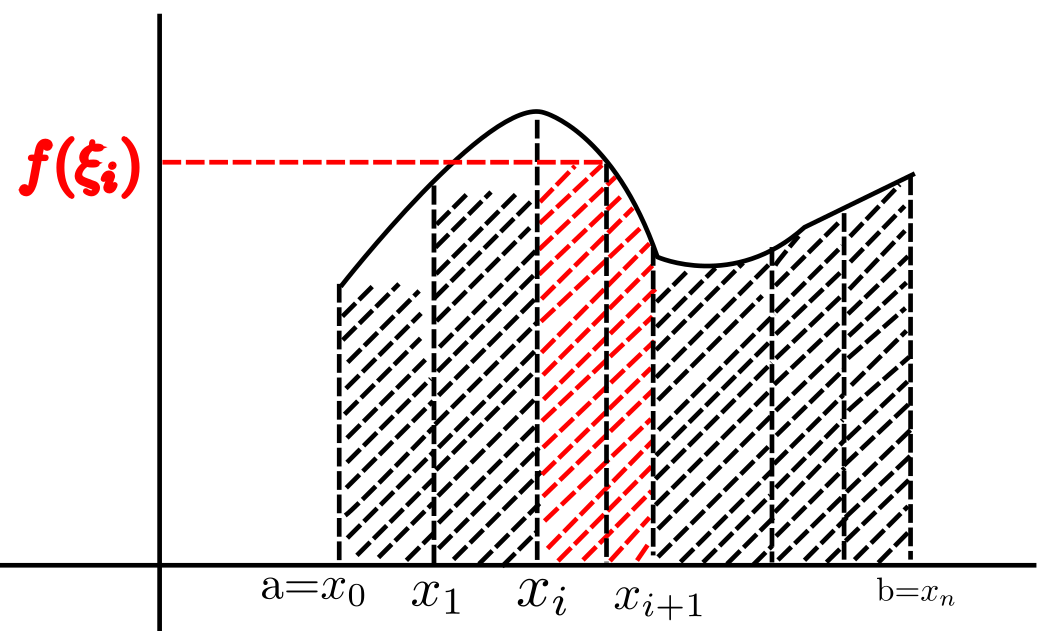
\includegraphics[width=0.8\linewidth]{6.1.1.png}
    \end{center}
    \indent $Пусть f(x)\geq 0$\\
    \begin{enumerate}
        \item Произведём разбиение [a;b] R\\ a=$x_0<x_1<\dots<x_n=b$
        \item В каждом элементарном отрезке [$x_i;x_{i+1}$] произвольным образом выберем (.) $\xi_i$
        \item Вычислим $f(\xi_i)$
        \item Вычислим $f(\xi_i) \Delta x_i$
        \item Вычислим $\sigma_r = \sum_{i=0}^{n-1} f(\xi_i) \Delta x_i$
        \item Обозначим $\lambda_R - диаметр разбиения\\ \sigma_r=[x_i;x_i+1]\\ Пусть \sigma_r \rightarrow 0 \\ Вычислим \lim_{n \to \inf} \sigma_R = S$
    \end{enumerate}
    
    \subsection*{2. Вычисление массы неоднородного тонкого стержня}
    \begin{center}
        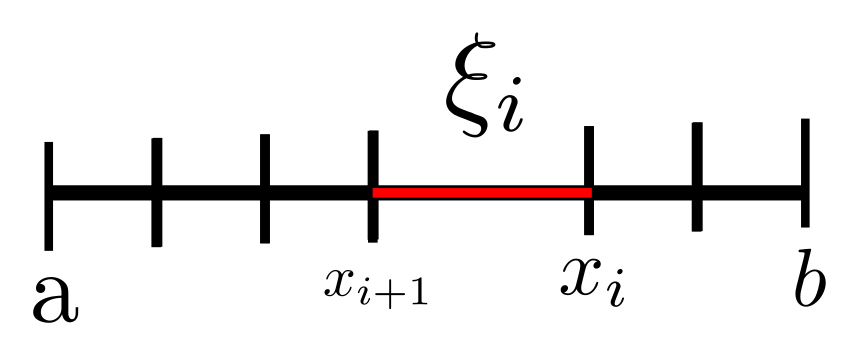
\includegraphics[width=0.8\linewidth]{6.2.1}
    \end{center}

    P$(\xi_i)$ Пусть $\rho = const = \rho (\xi_i) \forall x \in [x_i;x_{i+1}]$\\
    $m_i=\rho(\xi_i) \Delta x_i$\\ $m \approx \sum_{i} \rho(\xi_i) \Delta x_i=\delta_r; m=\lim_{n \to \inf} \delta_r$

    \subsection{Определение определённого интеграла}
    \indent Пусть на [a;b] задана ф-ия f(x)\\
    \begin{enumerate}
        \item Произведём разбиение отрезка [a;b]\\
        a=$x_0<x_1<\dots<x_n=b\,$ R Пусть $\lambda_r = \underset{i}{max}[x_i;x_{i+1}]$ - диаметр разбиения
        \item В каждом элементарном [$x_i;x_{i+1}$] произвольным образом выберем $\xi_i$
        \item Вычислим $f(\xi_i)\Delta x_i$
        \item Составим $\sigma_r=\sum_{i=0}^{n-1} f(\xi_i) \Delta x_i$ - интегральная сумма
        \item Если $\exists$ \underline{конечный} предел интегральной суммы $\sigma_r$ при $\lambda_r \to 0$,
        не зависящий от способа разбиения [a;b] и выбора (.) $\xi_i$, то он называется определённым интегралом
        от функции f(x) на [a;b]
    \end{enumerate}

    \underline{Обозначение} : $\lim_{\sigma_R \to 0} \delta_r = \int_{a}^{b} f(x)dx$

    \subsection*{Определение определённого интеграла на языке "$\varepsilon - \delta$"}
    \underline{Определение} : Число I называется определённым интегралом от функции f(x)
    на [a;b], если $\forall \varepsilon>0 \exists \delta = \delta(\varepsilon)>0: 
    \forall \lambda_r < \delta \Rightarrow 1I-\sigma_r | <\varepsilon$

    \subsection{Необходимое условие интегрируемости функции}
    \subsubsection*{Теорема 6.3.1}\label{th:6.3.1}
    Если функция интегрируема на некотором отрезке, то она ограничена на нем \par\noindent
    \underline{Доказательство:}
    \begin{adjustwidth}{1.5em}{1.5em}
        Пусть f(x) интегрируема на [a;b] и I = $\int_{a}^{b} f(x)dx$($\exists$ конечное число)\\
        Зафиксируем $\varepsilon$. Тогда по \underline{определению} $\exists \delta: \sigma_r<\delta \Rightarrow 1\delta_r - I|<\varepsilon$
        I-$\varepsilon<\sigma_r<I+\varepsilon$ - множество интегральных сумм\\ $\sigma_r$ ограничено
        Пойдем от противного: Пусть f(x) интегрируема на [a;b], но не ограничена на нём.\\
        Произведем разбиение R отрезка [a;b]\\
        Т.к. f(x) неограниченна на [a;b] $\Rightarrow$ f неограниченна по крайней мере на одном из элементарных отрезков [$x_i;x_{i+1}$]
        Пусть для определённости этот отрезок $[x_0;x_1]$. Тогда $\forall n \in N \exists(.) \xi^{(n)}_0
        :f(\xi^{(n)}_0)>n$, $\xi^{(n)}_0 \in [x_0;x_1]$\\
        Тогда $\lim_{n \to \inf} f(\xi^{(n)}_0) = \inf$\\
        Составим $\sigma_R$:\\
        $\sigma_R = f(\xi^{(n)}_0) \Delta x_o + \sum_{i=1}^{n} f(\xi_i) \Delta x_i$\\
        $\lim_{n \to inf} \sigma_r = \inf$; т.е. $\sigma_R$ неограниченна. Получили противоречие. f(x) ограничена
        \begin{center}
            \textbf{Ч.т.д.}
        \end{center}
    \end{adjustwidth}

    \underline{Замечание:} Ограниченность функции является необходимым условием, но не является достаточным.\\
    \indent Если функция ограничена, она не обязана быть интегрируемой!!!\\
    \underline{Пример:} Функция Дирихле́\\
    $f(x) = \begin{cases}
        1,x \in Q\\
        0,x \in I
    \end{cases}$
    \begin{enumerate}
        \item $[a;b]$ R\\
        Пусть (.) $\xi_i \in Q \Rightarrow f(\xi_i) = 1 \Rightarrow \sum_{i=0}^{n} f(\xi_i) \Delta x_i =
        \sum_{i=0}^{n} \Delta x_i = b-a$\\
        $\lim_{\lambda_R \to 0} \sigma_r = \lim_{\lambda_R \to 0} (b-a) = b-a$
        \item $[a;b]$ R\\
        Пусть (.) $\xi_i \in I \Rightarrow f(\xi_)i=0$\\
        $\sigma_R = \sum_{i=0}^{n} f(\xi_i) \Delta x_i =0$\\
        $\lim_{\lambda_R \to 0} \sigma_R = 0$\\
        $\lim_{\lambda_R \to 0} \sigma_R = \not \exists$
    \end{enumerate}

    \subsection{Суммы Дарбу}
    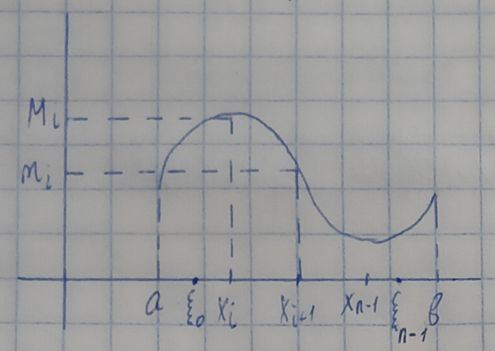
\includegraphics[width=0.8\linewidth]{6.4.1.png}\\
    Пусть f(x) задана на [a;b] и ограничена на нём\\
    R $a=x_0<x_1<\dots<x_n=b$\\
    Пусть $mi = \underset{x \in [x_i;x_{i+1}]}{inf f(x)}$, $Mi = \underset{x \in [x_i;x_{i+1}]}{sup f(x)}$
    Составим $\sigma_R = \sum_{i=0}^{n-1} f(\xi_i) \Delta x_i$\\
    Рассмотрим\\
    Суммы Дарбу $\begin{cases}
        \underline{S_r} = \sum_{i=0}^{n-1} mi \Delta x_i\\
        \overline{S_r} = \sum_{i=0}^{n-1} Mi \Delta x_i
    \end{cases}$\\
    Очевидно \underline{$S_R$}$\leq \sigma_R \leq \overline{S_r}$\\
    Суммы Дарбу - необязательно интегрируемые суммы\\
    \subsection*{Свойства сумм Дарбу:}
    \begin{enumerate}
        \item Нижняя (верхняя) сумма Дарбу является точный нижней (верхней) гранью интегральным сумм
        Римана, соответствующих данному разбиению R
        \underline{Доказательство:}
        \begin{adjustwidth}{1.5em}{1.5em}
            \underline{$S_R$} = $\sum_{i=0}^{n-1} mi \Delta x_i = \sum_{i=0}^{n-1}
            \underset{\xi_i \in \Delta x_i}{inf} f(\xi_i) \Delta x_i = \underset{\xi_i \in \Delta x_i}{inf}
            \sum_{i=0}^{n-1} f(\xi_i) \Delta x_i = \underset{\xi_i \in \Delta x_i}{inf} \sigma_R$
        \end{adjustwidth}
        \item Если к имеющимся у разбиения R точкам деления добавить новые точки, то верхняя сумма Дарбу
        не возрастает, а нижняя сумма Дарбу не убывает.\\
        \underline{Доказательство:}
        \begin{adjustwidth}{1.5em}{1.5em}
            \underline{Замечание:} для доказательства достаточно показать, что свойство выполняется при 
            добавлении одной (.)\\
            Пусть $\overline{S_R}$ - верхняя сумма Дарбу, отвечающая разбиению R\\
            Пусть $\overline{S_R}$ - верхняя сумма Дарбу, отвечающая разбиению R' R'=R+(.)\\
            $\overline{S_R}$ будет отличаться от $\overline{S_R}'$ тем, что вместо слагаемого Mi
            $\Delta x_i$ будут Mi'(x'-$x_i$)+Mi''($x_{i+1}-x'$)\\
            $M_i' = \underset{x \in [x_i;x']}{sup f(x)}$  $M_i''= \underset{x \in [x_i;x']}{sup f(x)}$\\
            Так как $[x_i;x'] \sqsubset [x_i;x_{i+1}]$\\
            $[x';x_{i+1}] \sqsubset [x_i;x_{i+1}]$, то $M_i' \leq M_i, M_i''\leq M_i$\\
            Получим что $M_i'(x'-x_i)+M_i''(x_{i+1}-x') \leq M_i(x'-x_i+x_{i+1}-x') = M_i(x_{i+1}-x_i)$\\
            Т. е. $\overline{S_r'} \leq \overline{S_r}$ Аналогично $\underline{S_R'} \leq \underline{S_R}$\\
            \begin{center}
                \textbf{Ч.т.д.}
            \end{center}
        \end{adjustwidth}
        \item Каждая нижняя сумма Дарбу не больше любой верхней\\
        \underline{Доказательство:}
        \begin{adjustwidth}{1.5em}{1.5em}
            Рассмотрим $R_1,R_2$ - различные разбиения\\
            Составим новое разбиение $R_3=R_1+R_2$\\
            $\underline{S_{R_1}} \underset{\text{св-во 2}}{\leq} \underline{S_{R_3}} \underset{\text{по определению}}{\leq} \overline{S_{R_3}} \leq \overline{S_{R_2}}$\\
            \begin{center}
                \textbf{Ч.т.д.}
            \end{center}
        \end{adjustwidth}
        \underline{Замечание:} Множество нижних сумм Дарбу \{$\underline{S_r}$\} всегда
        ограничено какой-либо верхней суммой Дарбу. Значит это множество ограничено сверху. Тогда существует
        точная верхняя грань множества нижних сумм Дарбу.\\
        $\underset{R}{sup} \underline{S_r} = I*$\\
        Аналогично $\exists I^* = \underset{R}{\text{inf}} \overline{S_r}$\\
        $I_* \leq I^* \forall R$\\
        $\underline{S_R} \leq I_* \leq I^* \leq \overline{S_R}$
        \item \subsubsection*{Теорема О существовании интеграла}\label{th:6.4.1}
        Для того, чтобы определённый интеграл, ограниченный функции f(x) существовал $\Leftrightarrow \lim_{\lambda_R \to 0} (\overline{S_r}-\underline{S_r})=0$,
        т.е. $\lim_{\lambda_R \to 0}\sum_{i=0}^{n-1} \omega_i \Delta x_i$ \par\noindent
        \underline{Доказательство:}
        \begin{adjustwidth}{1.5em}{1.5em}
            $\Rightarrow$ Пусть определённый интеграл от ограниченной функции f(x) существует на [a;b]\\
            Тогда $\lim_{\lambda_R \to 0} \sigma_R = I$, т.е. $\forall \varepsilon > 0 \exists \delta > 0:\lambda_R < \delta \Rightarrow 1 \sigma_R - I1 < \varepsilon$\\
            $I-\varepsilon < \sigma_R < I+\varepsilon \forall R$\\
            $\lim_{\lambda_R}(\overline{S_r}-\underline{S_r})=0\begin{cases}
                I-\varepsilon < \underline{S_r}<I+\varepsilon \Rightarrow \lim_{\lambda_R \to 0} \underline{S_r}=I\\
                I-\varepsilon < \overline{S_R} < I + \varepsilon \Rightarrow \lim_{\lambda_R} \overline{S_r} = I\\
            \end{cases}$\\
            $\Leftarrow$ Пусть $\lim_{\lambda_R \to 0}(\overline{S_r}-\underline{S_R})=0$\\
            Т. е. $\lim_{\lambda_R \to 0} \overline{S_R} = \lim_{\lambda_R \to 0} \underline{S_r}$\\
            $\{\overline{S_R}\}$ Невозрастающая, ограниченная снизу, те $\lim_{\lambda_R} \overline{S_R} = I^*$\\
            Аналогично $\lim_{\lambda_R} \underline{S_R} = I_*$. Тогда $I^* = I_* = I$\\
            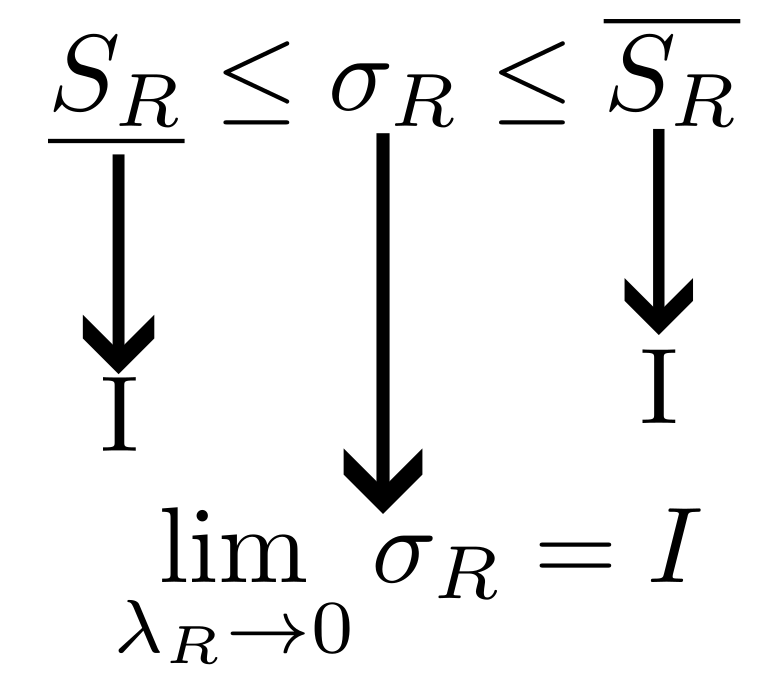
\includegraphics[width=0.8\linewidth]{6.4.2.png}
            \begin{center}
                \textbf{Ч.т.д.}
            \end{center}
        \end{adjustwidth}
    \end{enumerate}
    %параграф 5 дописать надо%
    \subsection{Достаточное условия интегрируемости функций}
    \subsubsection*{Теорема 6.5.1 }\label{th:6.5.1}
    Функция непрерывная на отрезке интегрируема на нем \par\noindent
    \underline{Доказательство:}
    \begin{adjustwidth}{1.5em}{1.5em}
        Если f(x) непрерывна на [a;b], то она равномерно непрерывна на нем.\\
        Тогда $\forall \varepsilon>0 \exists \delta'>0:\forall x',x'' \in [a;b]: |x'-x''|<\delta \Rightarrow |f(x')-f(x'')|<\varepsilon$\\
        Произведём разбиение R:$\lambda_R < \delta$\\
        Тогда $\forall x',x'' \in [x_i;x_{i+1}]|x'-x''|\leq x_{i+1}-x_i=\Delta x_i < \delta \Rightarrow |f(x')-f(x'')|<\varepsilon$\\
        Рассмотрим колебание функции f(x) на элементарном отрезке: $\omega_i=M_i-m_i = \underset{\Delta x_i}{sup}f(x)-\underset{\Delta x_i}{\text{inf}}f(x) \fbox{=}$\\
        \underline{Замечание:}
        \begin{math}
            \underset{[a;b]}{sup} \lambda f(x) = \lambda \underset{[a;b]}{\text{inf}} f(x),\lambda < 0\\
            \underset{[a;b]}{sup}(f(x)-g(x))=\underset{[a;b]}{sup} (f(x)+\underset{[a;b]}{sup} (-g(x))) = \underset{[a;b]}{sup} f(x)-\underset{[a;b]}{\text{inf}} g(x)\\
        \end{math}
        $\fbox{=} \underset{x',x'' \in \Delta x}{sup}|f(x')=f(x'')|<\varepsilon$\\
        \begin{center}
            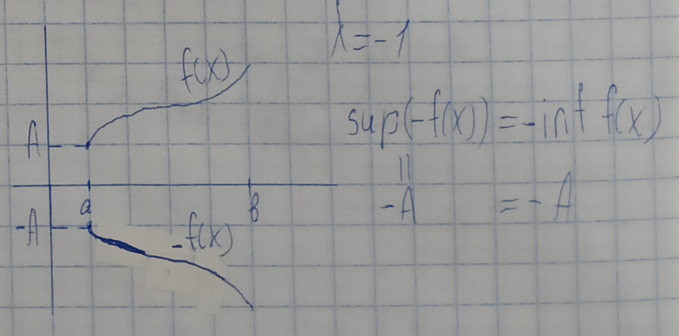
\includegraphics[width=0.6\linewidth]{6.5.1.png}\\
        \end{center}
        Рассмотрим $\sum_{i=0}^{n-1} \omega_i \Delta x_i < \varepsilon \sum_{i=0}^{n-1} \Delta x_i = \varepsilon (b-a)\\
        \lim_{\lambda_R \to 0} \sum_{i=0}^{n-1} \omega_i \Delta x_i = 0 \Rightarrow$ f(x) интегрируема на [a;b]\\
        \begin{center}
            \textbf{Ч.т.д.}
        \end{center}
    \end{adjustwidth}

    \subsubsection*{Теорема 6.5.2}\label{th:6.5.2}
    Ограниченная монотонная функция на отрезке, интегрируема на нём \par\noindent
    \underline{Доказательство:}
    \begin{adjustwidth}{1.5em}{1.5em}
        Пусть для определённости f(x) возрастает на [a;b]\\
        f(a)<f(x)<f(b) $\forall x \in (a;b)$\\
        \begin{math}
            m_i=\underset{[x_i;x_{i+1}]}{\text{inf}} f(x) = f(x_i)\\
            M_i = \underset{[x_i;x_{i+1}]}{sup}f(x)=f(x_{i+1})\\
            \overline{S_R}-\underline{S_r}=\sum_{i=0}^{n-1} (M_i-m_i) \Delta x_i = \sum_{i=0}^{n-1}(f(x_{i+1})-f(x_i))\Delta x_i < \sum_{i=0}^{n-1}(f(x_{i+1}-f(x_i)))\delta = (f(x_n)-f(x_o))\delta=(f(b)-f(a))\delta \fbox{=}\\
            \text{Пусть } \delta=\frac{f(b)-f(a)}{\varepsilon} \fbox{=} \varepsilon \\
        \end{math}
        Т.е. $\lim_{\lambda_R \to 0}(\overline{S_R}-\underline{S_R})=0$. Т.е.f(x) интегрируема на [a;b]
        \begin{center}
            \textbf{Ч.т.д.}
        \end{center}
    \end{adjustwidth}  
    \underline{Замечание:}
    Монотонные функции могут быть разрывными.\\
    Т.е. по   $\hyperref[th:6.5.2]{\text{Теореме 6.5.2 }} \exists$ разрывные интегрируемые функции\\
    \begin{center}
        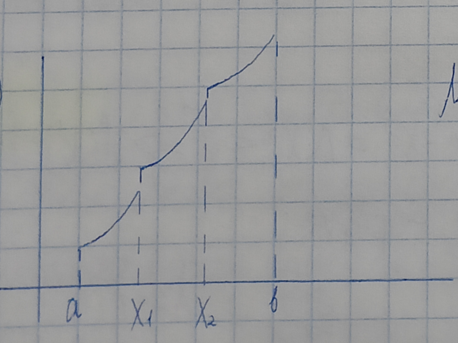
\includegraphics[width=0.5\linewidth]{6.5.2.png}
    \end{center}
    \subsection{Свойства интегрируемых функций}
    \begin{enumerate}
        \item $\int_{a}^{b} dx = b-a$\\
        $\int_{a}^{b} dx = \int_{a}^{b} 1*dx$\\
        $\sigma_R = \sum_{i=0}^{n-1} f(\xi_i)\Delta x_i=\sum_{i=0}^{n-1}\Delta x_i=b-a$\\
        $\lim_{\lambda_R \to 0} \sigma_R=b-a$
        \item Если f(x) интегрируема на каждом из [a;c],[c;b](a<c<b), то она интегрируема на [a;b]\\
        $\int_{a}^{b}f(x)dx=\int_{a}^{c}f(x)dx+\int_{c}^{b}f(x)dx$
        \underline{Доказательство:}\\
        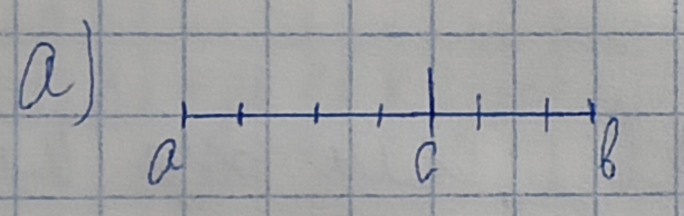
\includegraphics[width=0.5\linewidth]{6.6.1.png}\\
        \begin{adjustwidth}{1.5em}{1.5em}
            Произведем разбиение R[a;b]\\
            R:$a=x_0<x_1<\dots<x_m=c<\dots<x_n=b$\\
            Пусть $R_1: a=x_0<x_1<\dots<x_m=c$\\
            $R_2:c=x_m<x_{m+1}<\dots<x_n=b$\\
            Составим $\sigma_R$\\
            \begin{math}
                \sigma_R = \sum_{i=0}^{n-1}f(\xi_i)\Delta x_i=\sum_{i=0}^{m-1}f(\xi_i)\Delta x_i+\sum_{i=m}^{n-1}f(\xi_i)\Delta x_i=\sigma_{R_1}+\sigma{R_2}\\
                \lim_{\lambda_R \to 0}\sigma_R=\lim_{\lambda_R \to 0}(\sigma_{R_1}+\sigma_{R_2})=
                \begin{vmatrix}
                    \text{Если } \lambda_R \to 0 \Rightarrow \\
                    \lambda_{R_1} \to 0, \lambda_{R_2} \to 0
                \end{vmatrix}
                = \lim_{\lambda_R \to 0}\sigma_{R_1}=\lim_{\lambda_R \to 0}\sigma_{R_2}=
                \int_{a}^{c}f(x)dx+\int_{c}^{b}f(x)dx\\
            \end{math}
            \begin{center}
                a)
                \textbf{Ч.т.д.}
            \end{center}
            б) Пусть R - произвольное разбиение, не содержащее (.) C.\\
            R' - разбиение, содержащее (.) C.\\
            Пусть известно $\lim_{\lambda_R \to 0}\sigma_R'=I$. Покажет, что $\lim_{\lambda_R \to 0}\sigma_R=I \forall R$\\
            Пусть $R: a=x_0<x_1<\dots<\underset{x_m<c<x_{m+1}}{x_m<x_{m+1}}<x_n=b\\$
            \begin{center}
                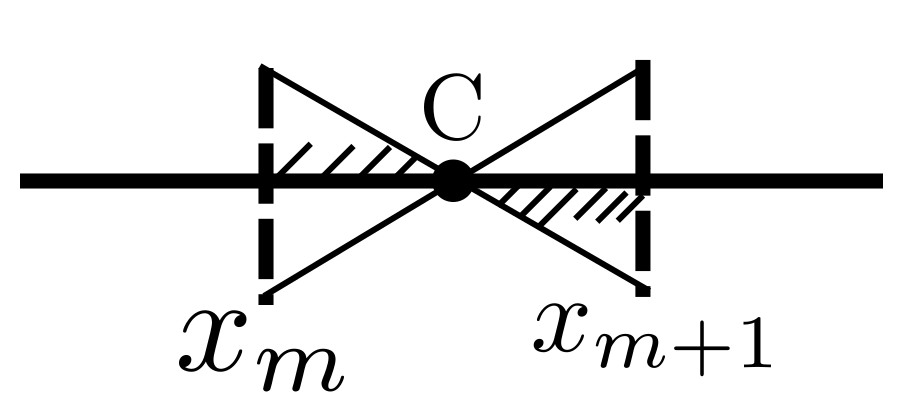
\includegraphics[width=0.5\linewidth]{6.6.2.png}
            \end{center}
            \begin{math}
                \sigma_R'=\sigma_R-f(\xi_m)(x_{m+1}-x+m)+f(\xi_m')(c-x_m)+f(\xi_m'')(x_{m+1}-c) \Rightarrow \sigma_R=\sigma_R'+A\\
                \text{Рассмотрим }|A|=|f(\xi_m)(x_{m+1}-x+m)+f(\xi_m')(c-x_m)+f(\xi_m'')(x_{m+1}-c)| \leq 
                |M(x_{m+1}-x_m)+M(c-x_m)+M(x_{m+1}-C)|=|2M(x_{m+1}-x_m)|\\ 
                \lim_{\lambda_R \to 0}|A|=0 \text{   } \lim_{\lambda_R \to 0} \sigma_R = \lim_{\lambda_R \to 0}(\sigma_R'+A)=
                \lim_{\lambda_R \to 0}\sigma_R'+\lim_{\lambda_R \to 0}A=
                \begin{vmatrix}
                    \text{Если } \lambda_R \to 0, \\
                    \text{то} \lambda_R' \to 0
                \end{vmatrix} 
                = \lim_{\lambda_R \to 0}\sigma_R' +\lim_{\lambda_R \to 0}A=I
            \end{math}
            \begin{center}
                \textbf{Ч.т.д.}
            \end{center}
        \end{adjustwidth}
        \textbf{Следствие:} Из 2 следует интегрируемость кусочно-непрерывных функций\\
        \underline{Определение:}
        Функция называется кусочно-непрерывной на [a;b] если она имеет на нём \underline{конечное} число (.) разрыв I рода\\
        На концах отрезка функция может быть не определена. Т.е. f(x) кусочно-непрерывна если \\$\exists R:\forall(.)x_k \text{   }k=\overline{0,n-1}$\\
        $\exists \text{ конечные пределы } \lim_{x \to x_k+0} f(x), \lim_{x\to x_k-0}f(x)$\\
        В (.) $x_k$ f(x) может быть определена или нет\\
        \begin{center}
            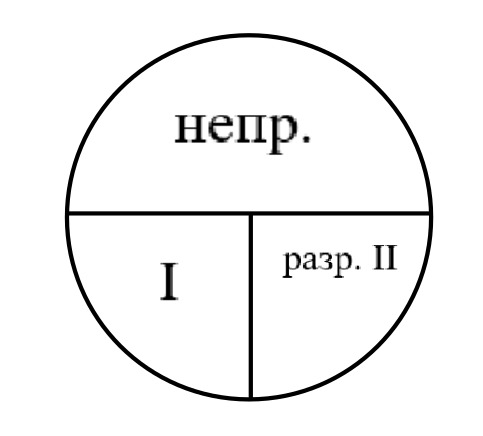
\includegraphics[width=0.4\linewidth]{6.6.3.png}\\
            \begin{math}
                f_k(x)=\begin{cases}
                f(x_k+0),x=x_k\\
                f(x),x_k<x<x_{k+1}\\
                f(x_{k+1}-0),x=x_k+1\\
            \end{cases}
            \end{math}
        \end{center}
        Тогда для таких функций свойство 2 выполняется $f_k$ в (.) $x_k$ может быть неопределенна.
        В этой случае нужно доопределить f(x) в этих (.). Т.е. $\int_{a}^{b} f(x) dx=\sum_{i=0}^{n-1}\int_{x_k}^{x_{k+1}}f_k(x)dx$
        \item Если функции f(x) и g(x) интегрируемы на [a;b],то $\forall \lambda , \mu$ функция $\lambda f-\mu g$ также интегрируема на [a;b].\\
        $\int_{a}^{b}[\lambda f(x) + \mu g(x)]dx=\lambda \int_{a}^{b}f(x)dx + \mu \int_{a}^{b} g(x) dx$\\
        \underline{Доказательство:}
        \begin{adjustwidth}{1.5em}{1.5em}
            Пусть R - произвольное разбиение\\
            $\sigma_R(\lambda f(x) + \mu g(x))=\sum_{i=0}^{n-1}(\lambda f(\xi_i) + \mu g(\xi_i))\Delta x_i = \lambda \sum_{i=0}^{n-1} f(\xi_i) \Delta x_i +
            \mu \sum_{i=0}^{n-1} g(\xi_i)\Delta x_i = \lambda \sigma_R(f)+\mu\sigma_R(g)$\\
            Т. К.f(x) и g(x) интегрируемы на [a;b] то существует конечный предел правой части => существует конечный 
            $\lim_{\lambda_R \to 0}\sigma_R (\lambda f + \mu g) = \lambda \lim_{\lambda_R \to 0}\sigma_R(f)+\mu \lim_{\lambda_R \to 0}\sigma_R(g)\\
            \int_{a}^{b}[\lambda f(x)+\mu g(x)]dx=\lambda \int_{a}^{b}f(x)dx+\mu \int_{a}^{b} g(x)dx$
            \begin{center}
                \textbf{Ч.т.д.}
            \end{center}
        \end{adjustwidth}
        \item Интегрируемость произведения интегрируемых функций: Если f(x) и g(x) интегрируемы на [a;b], то их произведение тоже интегрируемо.\\
        \underline{Доказательство:}
        \begin{adjustwidth}{1.5em}{1.5em}
            Если f(x) и g(x) интегрируемы на [a;b] то они ограничены на нём (необходимое условие интегрируемости).Т.е. $\forall
            x \in [a;b] |f(x)|\leq A,|g(x)|\leq A \Rightarrow |f(x)g(x)|\leq A^2,\text{Т.е. } |f(x)g(x)|$ ограничены.
            \underline{Замечание:} Рассмотрим 
            \begin{math}
                f(x')g(x')-f(x)g(x)=f(x')g(x')-f(x)g(x)-f(x)g(x')+f(x)g(x')=(f(x')-f(x)g(x'))+(g(x')-g(x))f(x)\\
                |f(x')g(x')-f(x)g(x)| \leq |f(x')-f(x)||g(x')|+|g(x')-g(x)||f(x)| \leq A(|f(x')-f(x)|+|g(x')-g(x)|)\\
            \end{math}
            Введем разбиение R и выберем (.) x и x' в одном и том же отрезке разбиения $[x_k;x_{k+1}]\\ \omega_k(fg)\leq A(\omega_k(f)+\omega_k(g))$\\
            Т.е. $\sum_{k=0}^{n-1} \omega_k (fg) \Delta x_k \leq A \sum_{k=0}^{n-1}\omega_k(f)\Delta x_k+\sum_{i=0}^{n-1}\omega_k(g)\Delta x_k$\\
            Переходя к lim при $\lambda_k \to 0$, получим $\lim_{\lambda_R \to 0} \sum_{k=0}^{n-1} \omega_k(fg) \Delta x_k=0$, Т.е.  f(x)g(x) интегрируема на [a;b] по \hyperref[th:6.4.1]{Теореме 6.4.1}\\
            \begin{center}
                \textbf{Ч.т.д.}
            \end{center}
        \end{adjustwidth}
        \item $\int_{a}^{a} f(x)dx=0 (\Delta x_i=0)$
        \item $\int_{a}^{b} f(x)dx=-\int_{b}^{a} f(x)dx(x_{k+1}-x_k=-(x_k-x_{k+1}))$
    \end{enumerate}
    \subsection{Оценки интегралов. Формулы среднего значения.}
    \begin{enumerate}
        \item Оценки интегралов:\\
        \begin{adjustwidth}{1.5em}{1.5em}
            a) Если f(x) интегрируема и $\forall x \in [a;b] f(x)\geq 0,\text{ то } \int_{a}^{b} f(x)dx \geq 0$
            \underline{Доказательство:}
            \begin{adjustwidth}{1.5em}{1.5em}
                Составим $\sigma_R=\sum_{k=0}^{n-1} f(\xi_k)\Delta x_k \geq 0\\
                \lim_{\lambda_R \to 0}\sigma_R=\int_{a}^{b}f(x)dx\geq 0$
                \begin{center}
                    \textbf{Ч.т.д.}
                \end{center}
            \end{adjustwidth}
            \textbf{Следствие:} Если f(x) и g(x) интегрируемы на [a;b] и $\forall x \in [a;b] f(x)\geq g(x), \text{ то } 
            \int_{a}^{b}f(x)dx \geq \int_{a}^{b} g(x)dx$\\
            \underline{Доказательство:}
            \begin{adjustwidth}{1.5em}{1.5em}
                Рассмотрим f(x)-g(x)$\geq 0 \overset{a)}{\Rightarrow} \int_{a}^{b} (f(x)-g(x))dx \geq 0 \\
                \int_{a}^{b} f(x)dx-\int_{a}^{b}g(x)dx\geq 0 \text{ (св-во 3) } \Rightarrow \int_{a}^{b}f(x)dx\geq\int_{a}^{b}g(x)dx$
                \begin{center}
                    \textbf{Ч.т.д.}
                \end{center}
            \end{adjustwidth}
            б) Если f(x) интегрируема на [a;b], то |f(x)| тоже интегрируема на [a;b] и $|\int_{a}^{b}f(x)dx|\leq \int_{a}^{b}|f(x)| dx$\\
            \underline{Доказательство:}
            \begin{adjustwidth}{1.5em}{1.5em}
                \begin{math}
                    \sigma_R=\sum_{k=0}^{n-1} f(\xi_k)\Delta x_k\\
                    |\sigma_R|=|\sum_{k=0}^{n-1} f(\xi_k)\Delta x_k| \leq \sum_{k=0}^{n-1}|f(\xi_k)|\Delta x_k
                    =\sigma_R(|f|)\\
                    \lim_{\lambda_R \to 0}|\sigma_R|=|\int_{a}^{b}f(x)dx|\leq \lim_{\lambda_R \to 0}\sigma_R (|f|)=\int_{a}^{b}|f(x)|dx\\
                \end{math}
            \end{adjustwidth}
        \end{adjustwidth}
        \item Непрерывность интегралов:\\
        \underline{Определение: } Функция F(x) = $\int_{a}^{x}f(t)dt$ - функция с переменным верхним пределом\\
        \begin{center}
            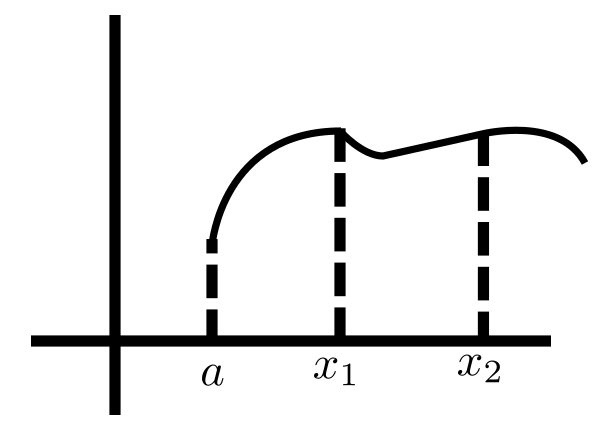
\includegraphics[width=0.6\linewidth]{6.7.1.png}
        \end{center}
        Аналогично G(x) = $\int_{x}^{b}f(t)dt$ - функция с переменным нижним пределом
        \subsubsection*{Теорема 6.7.1}\label{th:6.7.1}
        Если функция f(x) интегрируема на [a;b], то F(x),G(x) непрерывна на [a;b].\par\noindent
        \underline{Доказательство:}
        \begin{adjustwidth}{1.5em}{1.5em}
            Д-во проведем для F(x)\\
            f(x) ограничена на [a;b] (необходимое условие интегрируемости), Т.е. $\forall x \in [a;b]\\ |f(x)|\leq C\\
            F(x+\Delta x)=\int_{a}^{x+\Delta x}f(t)dt=\int_{a}^{x}f(t)dt = \int_{a}^{x} f(t)dt+\int_{x}^{x+\Delta x}f(t)dt$\\
            Рассмотрим $\Delta F(x) = F(x + \Delta x) - F(x)=\int_{a}^{x} f(t)dt+\int_{x}^{x+\Delta x}f(t)dt-\int_{a}^{x}f(t)dt=
            \int_{x}^{x+\Delta x}f(t)dt\\
            |\Delta F(x)| = | \int_{x}^{x+\Delta x }f(x)dt| \leq C |\int_{x}^{x+\Delta x}dt|=C|\Delta x|\\
            \lim_{\Delta x \to 0}|\Delta F(x)| = 0 \Rightarrow \lim_{\Delta x \to 0}\Delta F(x)=0 \Rightarrow$F(x) непрерывна в (.) X\\
            Т.К. x- производная в (.) [a;b] $\Rightarrow$F(x) непрерывна на [a;b]
            \begin{center}
                \textbf{Ч.т.д.}
            \end{center}
            \textbf{Следствие:} Если f(x) интегрируема на [a;b](и непрерывна на нём), то $\lim_{\varepsilon \to 0} \int_{a+\varepsilon}^{b-\varepsilon}
            f(x)dx=\int_{a}^{b}f(x)dx$\\
            \underline{Доказательство:}
            \begin{adjustwidth}{1.5em}{1.5em}
                \begin{math}
                    \lim_{\varepsilon \to 0} \int_{a+\varepsilon}^{b-\varepsilon}f(x)dx = \lim_{\varepsilon \to 0}(\int_{a+\varepsilon}^{C}f(x)dx+\int_{C}^{b-\varepsilon}f(x)dx) =
                    \lim_{\varepsilon \to 0} \int_{a+\varepsilon}^{C} f(x)dx+\lim_{\varepsilon \to 0}\int_{c}^{b-\varepsilon}f(x)dx=
                    \int_{a}^{c} f(x)dx+\int_{c}^{b} f(x)dx = \int_{a}^{b}f(x)dx
                \end{math}
                \begin{center}
                    \textbf{Ч.т.д.}
                \end{center}
            \end{adjustwidth}
        \end{adjustwidth}
        \subsubsection*{Теорема 6.7.2 Интегральная теорема о среднем}\label{th:6.7.2}
        Пусть f(x) и g(x) интегрируемы на [a;b] $\forall x \in [a;b] m \leq f(x) \leq M$ g(x) не меняет знак на [a;b]\\ Тогда $\exists \mu : m\leq \mu \leq M: 
        \int_{a}^{b} f(x)g(x)dx = \mu \int_{a}^{b}g(x)dx$\par\noindent
        \underline{Доказательство:}
        \begin{adjustwidth}{1.5em}{1.5em}
            \begin{math}
                m \leq f(x) \leq M | * g(x)\\
                g(x)\geq 0 : mg(x)\leq f(x)g(x)\leq Mg(x) \Rightarrow m \int_{a}^{b} g(x) dx \leq \int_{a}^{b}f(x)g(x)dx \leq M \int_{a}^{b}g(x)dx | : \int_{a}^{b} g(x)dx\\
                g(x)\leq 0 : mg(x)\geq f(x)g(x)\geq Mg(x) \Rightarrow m \int_{a}^{b} g(x) dx \geq \int_{a}^{b}f(x)g(x)dx \geq M \int_{a}^{b}g(x)dx | : \int_{a}^{b} g(x)dx\\
                \text{Если } \int_{a}^{b} g(x)dx = 0 \Rightarrow \int_{a}^{b} f(x)g(x)dx =0 \text{ в обоих случаях и } \mu \text{ любое} 
            \end{math}
            \begin{center}
                \textbf{Ч.т.д.}
            \end{center}
            Если $\int_{a}^{b} g(x) dx \not = 0$ при $\Rightarrow  \underset{g(x)<0 \Rightarrow \int_{a}^{b} g(x)dx<0}{g(x) > 0 \int_{a}^{b} g(x)dx >0} $\\
            Разделим на $\int_{a}^{b} g(x)dx,$ в обоих случаях получим: $m \leq \frac{\int_{a}^{b}f(x)g(x)dx}{\underset{\mu}{\int_{a}^{b}g(x)dx}}\leq M\\
            m\leq \mu \leq M \text{   } \int_{a}^{b} f(x)g(x)dx=\mu\int_{a}^{b}g(x)dx$
            \begin{center}
                \textbf{Ч.т.д.}
            \end{center}
            \textbf{Следствие:} При дополнительно условии о том, что f(x) непрерывна на [a;b], тогда на (a;b) $\exists (.) \xi:\int_{a}^{b}f(x)g(x)dx=f(\xi)\int_{a}^{b}g(x)dx$\\
            В частности, пусть $g(x)=1 \text{   } \int_{a}^{b} f(x) dx=f(\xi)(b-a) \Rightarrow f(\xi)=\frac{1}{b-a}\int_{a}^{b}f(x)dx$ - формула среднего значения\\
            $f(\xi)=\frac{\int_{a}^{b} f(x)dx}{b-a}$\\
            \begin{center}
                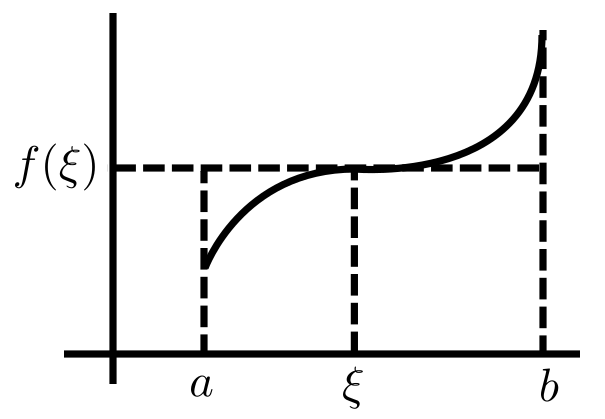
\includegraphics[width=0.7\linewidth]{6.7.2.png}
            \end{center}
            \underline{Доказательство:}
            \begin{adjustwidth}{1.5em}{1.5em}
                Если $\int_{a}^{b} g(x)dx=0,$ то верно $\forall \xi$\\
                Пусть $\int_{a}^{b} g(x)dx \not = 0$ и для определенности g(x)>0,$\underset{m=\underset{x \in [a;b]}{\text{inf}}f(x) M=\underset{x \in [a;b]}{sup}f(x)}{m\leq f(x) \leq M}$\\ 
            \end{adjustwidth}
            и по \hyperref[th:6.7.2]{Теореме 6.7.2} $m \leq \mu \leq M$\\
            \begin{enumerate}
                \item Случай: Пусть $m<\mu<M$\\
                По 2-ой теореме Вейерштрасса $\exists \alpha, \beta \in [a;b]: f(\alpha) = m,f(\beta) = M$\\
                Тогда по Теореме Больцано-Коши $\exists (.) \xi:\underset{m<\mu <M \text{   } \mu=f(\xi)}{m<f(\xi)<(M)}$
                \begin{center}
                    \textbf{Ч.т.д.}
                \end{center}
                \item Случай: $\mu=M \text{ или } \mu=m$\\
                Пусть для определенности $\mu=M$\\
                Покажем, что и в этом случае на (a;b) $\exists (.) \xi: f(\xi)=\mu=M$\\
                Пойдем от противного: Пусть на (a;b) $\not \exists (.) \xi:f(\xi)=\mu=M.$ Тогда своего наибольшего значения
                f(x) достигает в какой-либо (.) или x=a или x=b\\
                Рассмотрим [$a+\varepsilon;b-\varepsilon$] f(x) непрерывна на нём $\Rightarrow$ по 2-ой Теореме Вейерштрасса\\
                Пусть (.) $x_0$, в которой f(x) достигает своего наибольшего значения.\\
                Тогда $M-f(x_0)=\underset{x \in [a+\varepsilon;b-\varepsilon]}{min}f(x)$\\
                Т.К. $\mu=M,$ то по \hyperref[th:6.7.2]{Теореме 6.7.2} $\int_{a}^{b} f(x)g(x)dx=M\int_{a}^{b}g(x)dx \Rightarrow \int_{a}^{b}
                (M-f(x))g(x)dx=0$\\
                Рассмотрим $\int_{a}^{b}(M-f(x))g(x)dx\geq\int_{a+\varepsilon}^{b-\varepsilon}(M-f(x))g(x)dx \geq (M-f(x_0)) \underset{>0}{\int_{a+\varepsilon}^{b-\varepsilon} g(x)dx>0}$ Получили противоречие
                $\Rightarrow \exists (.) \xi \in (a;b): f(\xi)=M=\mu$\\
                \begin{center}
                    \textbf{Ч.т.д.}
                \end{center}
            \end{enumerate}
        \end{adjustwidth}
        \subsubsection*{Теорема 6.7.3 Дифференцирование интеграла по верхнему пределу}\label{th:6.7.3}
        Если f(x) интегрируема на [a;b] и непрерывна в (.) $x_0 \in [a;b]$, то $F(x)=\int_{a}^{x}f(t)dt$ дифференцируема в этой (.) и F'($x_0$)=f($x_0$) \par\noindent
        \underline{Доказательство:}\\
        \begin{adjustwidth}{1.5em}{1.5em}
            \begin{math}
                \lim_{\Delta x \to 0}  \frac{\Delta F}{\Delta x} = F'(x_0)\\
                \Delta F=\int_{x_0}^{x_0+\Delta x}f(t)dt \text{   } x_0 \in [a;b],x_0+\Delta x \in [a;b]\\
                \frac{1}{\Delta x}\int_{x_0}^{x_0+\Delta x}dt=1\\
                \text{\underline{Замечание: } Рассмотрим} |\frac{\Delta F}{\Delta X}-f(x_0)| = |\frac{1}{\Delta x}\int_{x_0}^{x_0+\Delta x}f(t)dt-\frac{f(x_0)}{\Delta x}\int_{x_0}^{x_0+\Delta x}dt|=
                |\frac{1}{\Delta x}\int_{x_0}^{x_0+\Delta x}(f(t)-f(x_0))dt| \leq \frac{1}{|\Delta x|}\int_{x_0}^{x_0+\Delta X}|f(t)-f(x_0)|dt| \fbox{<}\\
                \text{Т.к. f(x) непрерывна в (.) $x_0$, то} \forall \varepsilon > 0 \exists \delta>0:|x-x_0|<\delta \Rightarrow |f(x)-f(x_0)|<\varepsilon\\
                \text{Пусть $|\Delta x| < \delta$. Тогда } \forall t \in [x_0;x_0+\Delta x]\\
                |t-x_0|\leq|\Delta x| < \delta \Rightarrow |f(t)-f(x_0)| < \varepsilon\\
                \fbox{<} \frac{\varepsilon}{\Delta x}|\int_{x_0}^{x_0+\Delta x}dt|=\varepsilon. \text{Т.е. } \lim_{\Delta x \to 0} \frac{\Delta F}{\Delta x} = F'(x_0)=f(x_0)
            \end{math}
            \begin{center}
                \textbf{Ч.т.д.}
            \end{center}
        \end{adjustwidth}
        \underline{Замечание:} Рассмотрим
        \begin{math}
            \int_{a}^{b} f(x)dx=\int_{a}^{b}f(t)dt\\
            \int_{a}^{b} f(t)dt=\int_{a}^{x}f(t)dt+\int_{x}^{b} f(t)dt \text{   } x \in (a;b)\\
            \int_{a}^{b} f(t) dt = F(x)+G(x) \text{   } G'(x)=-F'(x)\\
            0=F'(x)+G'(x)\text{   }G'(x_0)=-F'(x_0)=-f(x_0)
        \end{math}
    \end{enumerate}
    \subsection{Существование первообразных для непрерывных функций. \\Основные правила интегрирования}
    \subsubsection*{Теорема 6.8.1 О Существовании первообразных для непрерывной функции}\label{th:6.8.1}
    Если f(x) непрерывна $\forall x \in [a;b],$ то на [a;b] у нее существует первообразная\\
    Если $x_0$ - производная: $x_0 \in [a;b]$, то $F(x)=\int_{x_0}^{x}f(t)dt $ является одной из первообразных на [a;b]\par\noindent
    \underline{Доказательство:}
    \begin{adjustwidth}{1.5em}{1.5em}
        Для доказательства надо показать, что F'(x)=f(x). \hyperref[th:6.7.3]{Теорему 6.7.3}\\
        ()$F'(x_0)=f(x_0)$. Но так как $x_0$ - производная: $x_o \in [a;b],$ то это равенство выполняется $\forall x \in [a;b]$)
    \end{adjustwidth}
    \begin{center}
        \textbf{Ч.т.д.}
    \end{center}
    \underline{Замечание:}$F(x)=\int_{x_0}^{x}f(t)dt$\\
    Если $x>x_0, F'(x)=f(x)$\\
    Если $x<x_0, F'(x)=[\underset{G(x)}{\underline{-\int_{x}^{x_0}f(t)dt}}]=-(-f(x))=f(x)$\\
    \underline{Замечание:}$\int f(x)dx=F(x)+C$\\
    $\underset{\text{связь между неопределенным и определённым интегралом}}{\int f(x)dx = \int_{x_0}^{x}f(t)dt+C}$
    \subsubsection*{Теорема 6.8.2 Основная теорема интегрального исчисления}\label{th:6.8.2}
    Если f(x) непрерывна на [a;b], то какова бы не была на [a;b] её первообразная Ф(x), то справедлива формула 
    $\int_{a}^{b}f(x)dx=$Ф(x)$\Big|^{b}_{a}=$Ф(b)-Ф(a)- функция Ньютона-Лейбница \par\noindent
    \underline{Доказательство:}\\
    \begin{adjustwidth}{1.5em}{1.5em}
        По \hyperref[th:6.8.1]{Теореме 6.8.1} F(x)=$\int_{a}^{x} f(t)dt$ - является первообразной для f(x) на [a;b]\\
        Т.к. F(x) и Ф(x) - две первообразные для одной и той же f(x) на [a;b], то \\
        \begin{math}
            F(x)=\text{Ф(x)}+C\\
            \int_{a}^{x}f(t)dt = \text{Ф(x)+C}\\
        \end{math}
        Пусть x=a 0=Ф(а)+С $\Rightarrow C=-$Ф(а). Тогда $\int_{a}^{x}f(t)dt=$Ф(x)-Ф(а)\\
        Пусть x=b $\int_{a}^{b} f(t)dt=$Ф(b)-Ф(а)\\
        Если переобозначить, то $\int_{a}^{b}f(x)dx=F(b)-F(a)$
    \end{adjustwidth}
    \begin{center}
        \textbf{Ч.т.д.}
    \end{center}
    \subsubsection*{Теорема 6.8.3 Замена переменной в определённом интеграле}\label{th:6.8.3}
    Пусть f(x) задана на $\Delta x,x=\phi(t)$ задана на $\Delta t$. $\phi(\Delta t) \subset \Delta x$, Т.е. задана сложная функция ($f(\phi(t))$). Если f(x) непрерывна на 
    $\Delta t$, то $\int_{a}^{b}f(x)dx=\int_{a}^{x}f(\phi(t))\phi'(t)dt, a=\phi(\alpha),b=\phi(\beta)$\par\noindent
    \underline{Доказательство:}
    \begin{adjustwidth}{1.5em}{1.5em}
        Пусть F(x) - является первообразной для f(x) на [a;b]\\
        $\int_{a}^{b} f(x)dx=F(x)\Big|^{b}_{a}$\\
        $(F(\phi(t)))'=F'(\phi(t))\phi'(t)=f(\phi (t))\phi'(t)$\\
        Т.е. $F(\phi(t))$ является первообразной для $f(\phi(t))\phi'(t) $ на [$\alpha;\beta$]\\
        $\int_{\alpha}^{\beta}f(\phi(t))\phi'(t)dt=F(\phi(t))\Big|^{\beta}_{\alpha}=F(\phi(\beta))-F(\phi(\alpha))=F(b)-F(a)=\int_{a}^{b}f(x)dx$
    \end{adjustwidth}
    \begin{center}
        \textbf{Ч.т.д.}
    \end{center}
    \subsubsection*{Теорема 6.8.4 Формула интегрирования по частям}\label{th:6.8.4}
    Если u(x),u'(x),v(x),v'(x) непрерывна на [a;b] то $\int_{a}^{b} udv = uv \Big|^b_a-\int_{a}^{b}vdu$\par\noindent
    \underline{Доказательство:}
    \begin{adjustwidth}{1.5em}{1.5em}
        $(uv)'=u'v+uv'\\ \int_{a}^{b} (uv)'dx=\int_{a}^{b} u'v dx+\int_{a}^{b}uv'dx\\ uv \Big|^b_a=\int_{a}^{b}vdu + \int_{a}^{b} udv\\
        \int_{a}^{b}udv=uv\Big|^b_a-\int_{a}^{b} vdu$
    \end{adjustwidth}
    \begin{center}
        \textbf{Ч.т.д.}
    \end{center}
    \subsection{Геометрические приложения определённого интеграла. Площадь криволинейной трапеции}
    \begin{enumerate}
        \item f(x) задана явно на [a;b], пусть f(x) $\geq 0$\\
        $R: a=x_0<x_1<\dots<x_n=b$\\
        В каждом $[x_i;x_{i+1}]$ произвольно (.)$\xi_i$. Вычислим f($\xi_i$). Вычислим $f(\xi_i)\Delta x_i$.\\
        Составим $\sigma_R=\sum_{i=0}^{n-1}f(\xi_i)\Delta x_i\\
        \lim_{\lambda_R \to 0}\sigma_R=\int_{a}^{b} f(x)dx=S\\ S=S_1+S_2+S_3$
        \begin{center}
            $S=S_1+S_2+S_3$\\
            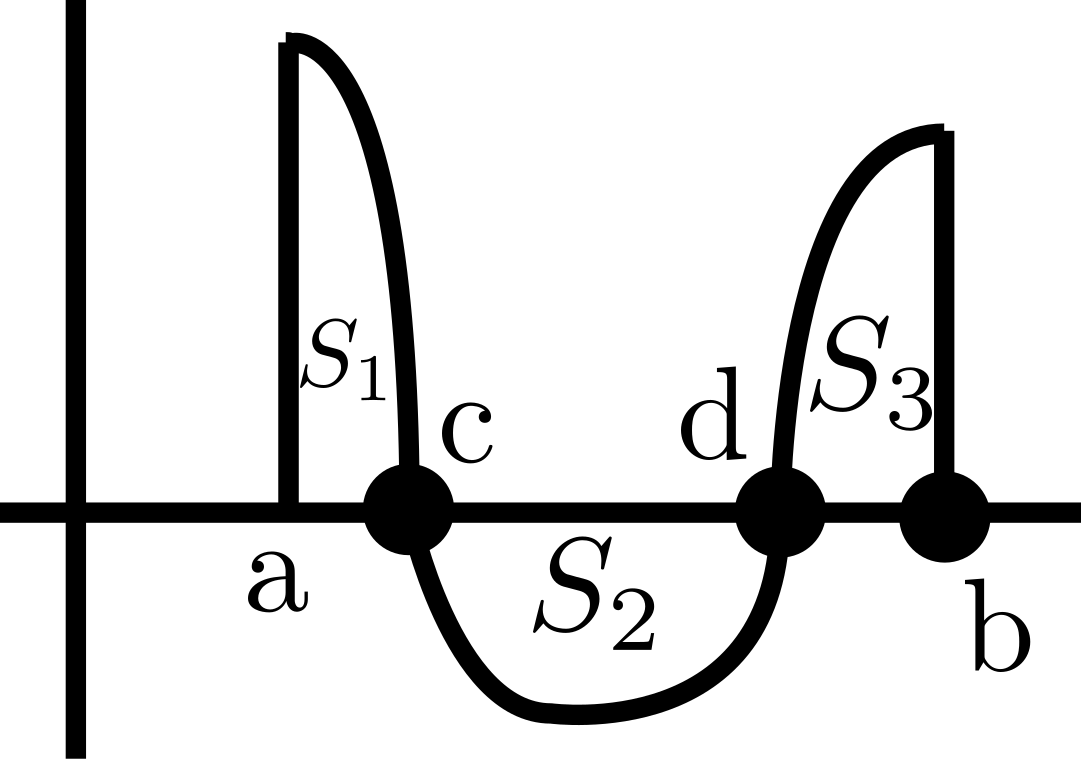
\includegraphics[width=0.6\linewidth]{6.9.1.png} 
        \end{center}
        \begin{center}
            S=$\int_{a}^{b}(\underset{большая}{f_1(x)} -  \underset{меньшая}{f_2(x)})dx$\\
            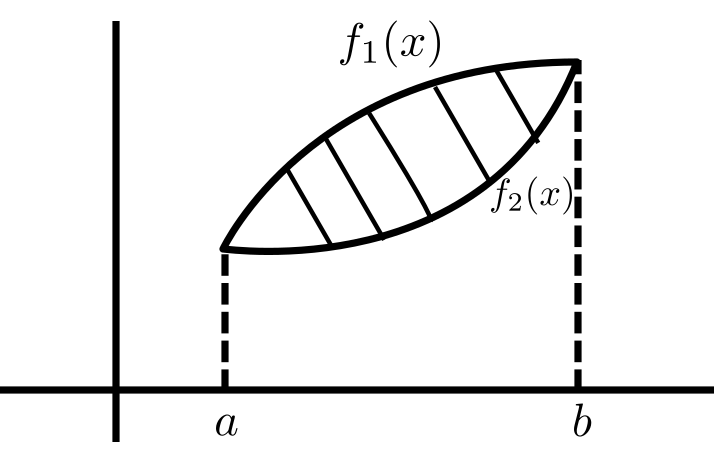
\includegraphics[width=0.7\linewidth]{6.9.2.png}
        \end{center}
        \item Если функция задана параметрически\\
        $\begin{cases}
            x=(t)\\
            y=y(t)
        \end{cases} \alpha \leq t \leq \beta$\\
        $\begin{cases}
            x=cos(t)\\
            y=sin(t)
        \end{cases} 0 \leq t \leq 2 \pi$\\
        S=$\int_{a}^{b} f(x)dx = \int_{a}^{b} ydx=
        \begin{vmatrix}
            x=x(t)\\
            a=x(\alpha)\\
            b=x(\beta)
        \end{vmatrix} = $\fbox{$\int_{a}^{b}y(t)x'(t)dt=S$}
        \item Вычисление S криволинейной трапеции в полярной системе координат. \\ Полярная система координат:
        \begin{center}
            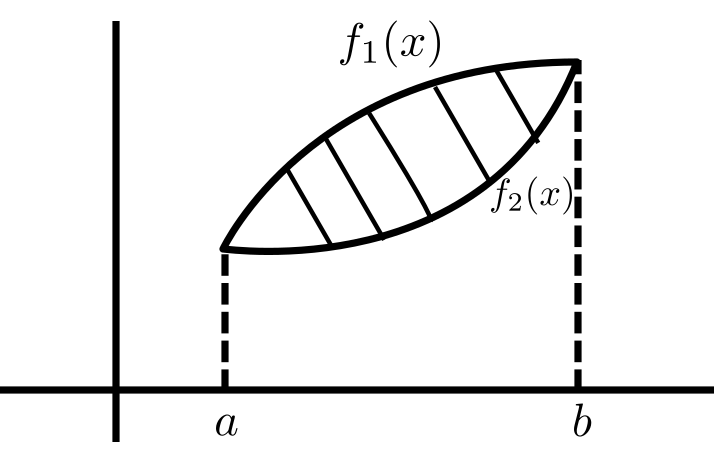
\includegraphics[width=0.9\linewidth]{6.9.3.png}\\
        \end{center}
        Некоторые кривые в полярной системе координат:
        \begin{center}
            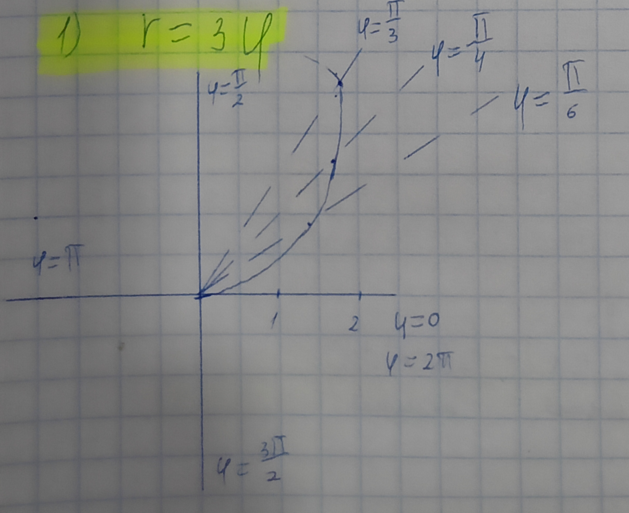
\includegraphics[width=0.7\linewidth]{6.9.4.png}\\
        \end{center}
        \begin{center}
            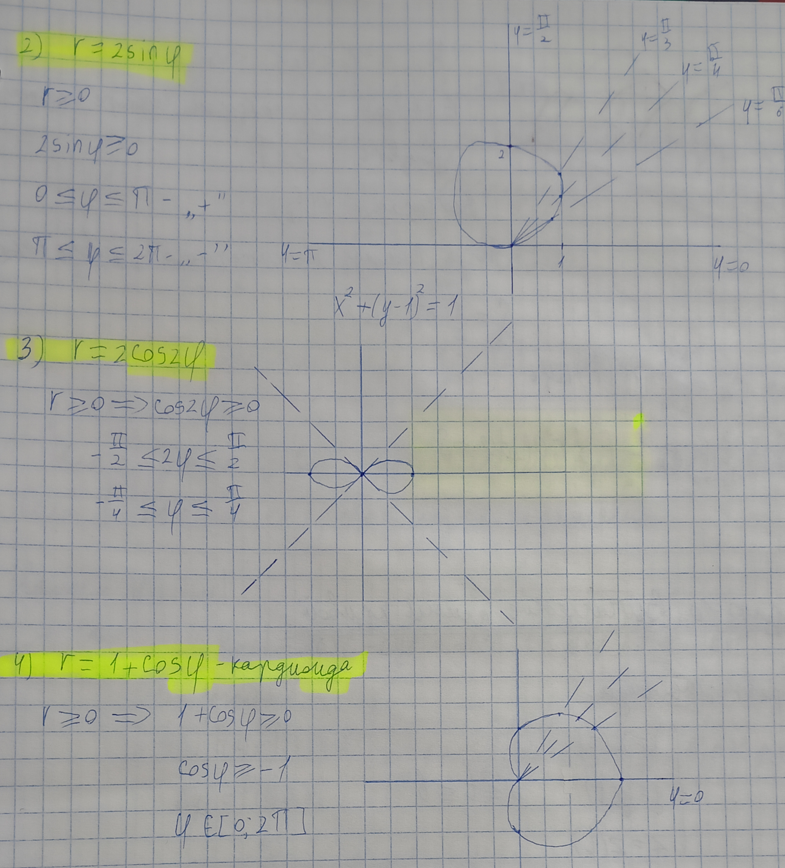
\includegraphics[width=0.9\linewidth]{6.9.5.png}\\
        \end{center}
        \underline{Площадь криволинейной трапеции в полярной системе координат:}\\
        Найти площадь криволинейной сектора, ограниченного дугой\\
        r$=r(\phi)$ и двумя полярными радиусами $\phi = \alpha$ и $\phi = \beta$\\
        $R: \alpha=\phi_0<\phi_1<\dots<\phi_n=\beta$\\
        В каждом элементарном секторе выберем произвольно:$\phi=\xi_i$\\
        Вычислим $r(\xi_i)$\\
        Тогда площадь элементарного кругового сектора: $S_i=\frac{1}{2} r^2(\xi_i) \Delta \phi_i$\\
        Составим $\sigma_R=\sum_{i=0}^{n-1} \frac{1}{2} r^2(\xi_i) \Delta \phi_i$\\
        Тогда $S=\lim_{\lambda_R \to 0}\sigma_r = \int_{a}^{b}\frac{1}{2} r^2(\xi_i) \Delta \phi_i=S$
        \begin{center}
            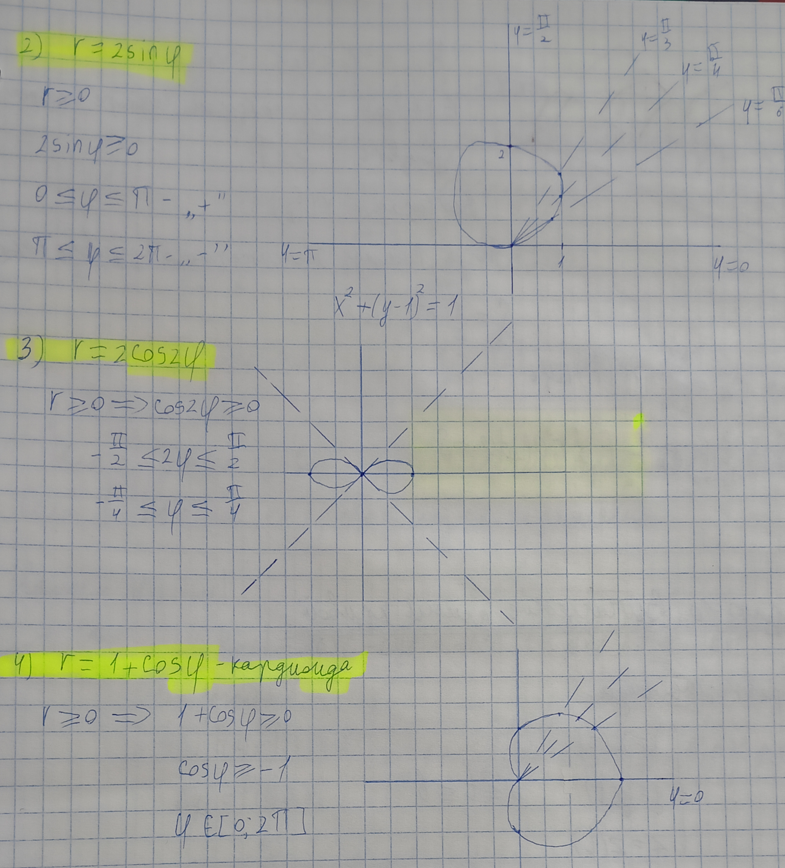
\includegraphics[width=0.7\linewidth]{6.9.6.png}
        \end{center}
    \end{enumerate}
    \subsection{Вычисление длины кривой.}
    \underline{Определение: } Уравнения вида: $\begin{cases}
        x=x(t)\\
        y=y(t)\\
        z=z(t)
    \end{cases} a\leq t \leq b$\\
    Где x(t),y(t),z(t) непрерывны определяют в пространстве непрерывную кривую Г\\
    \underline{Определение: } если функции x(t),y(t),z(t) не точно непрерывны, но и имеют непрерывные x'(t),y'(t),z'(t),
    одновременно не образующиеся в ноль $\forall t \int [a;b] (x'(t)^2,y'(t)^2,z'(t)^2 \ne 0), $ то кривая называется гладкой.\\
    $R:a=x_0<x_1<\dots<x_n=b$\\
    Каждой (.) $x_i$ на кривой соответствует $(.) M_i$. Соединим все соседние (.) ломанными $M_i,M_{i+1}$.\\
    $|\text{Г}_n|=\sum_{i=0}^{n-1}|M_iM_{i+1}|$
    \begin{center}
        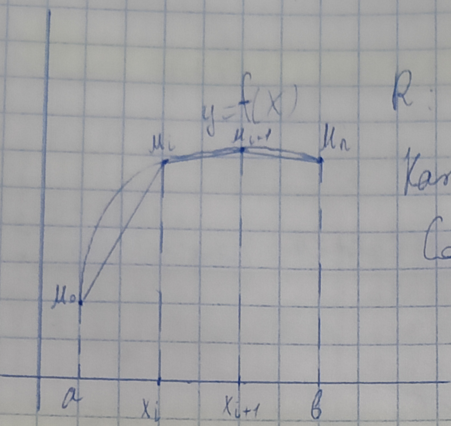
\includegraphics[width=0.5\linewidth]{6.10.1.png}
    \end{center}
    \underline{Определение: } Если существует конечный предел $\lim_{\lambda_R \to 0} |\text{Г}_n|$, то он называется длиной кривой y=f(x) на [a;b].\\
    Или: длина кривой - точная верхняя грань $|\text{Г}_n|$. l=sup|$\text{Г}_n$|. Если l - конечное, то кривая называется спрямляемой.\\
    Найдем |$M_iM_{i+1}$|.\\
    |$M_iM_{i+1}$|=$\sqrt{\Delta x_i^2+\Delta y_i^2}=\sqrt{\Delta x_i^2(1+\frac{\Delta y_i^2}{\Delta x_i^2})}+\sqrt{1+\frac{\Delta y_i^2}{\Delta x_i^2}}*\Delta x_i=
    \begin{vmatrix}
        \text{Теорема Лагранжа}\\
        f(b)-f(a)=f'(\xi)(b-a)\\
        \Delta y_i=f'(\xi)\Delta x_i
    \end{vmatrix}=\sqrt{1+\frac{f'(\xi)^2 \Delta x_i^2}{\Delta x_i^2}}\Delta x_i=\sqrt{1+f'(\xi_i)^2}\Delta x_i$\\
    Составим $\sigma_R=\sum_{i=0}^{n-1}\sqrt{1+f'(\xi_i)^2}\Delta x_i$\\
    \underline{Замечание:} (.) $\xi_i$ берется из Теоремы Лагранжа, но можно показать, что lim будет существовать при произвольном
    выборе $(.) \xi_i$\\
    Тогда $\lim_{\lambda_R \to 0} \sigma_R = l =\int_{a}^{b} \sqrt{1+y'(x)^2}dx$
    \subsection*{Длина дуги для функции, заданной параметрически:}
    \begin{math}
        \text{Пусть } \begin{cases}
            x=x(t)\\
            y=y(t)
        \end{cases} \alpha \leq t \leq \beta \text{  Пусть  } x(\alpha)=a,x(\beta)=b\\
        \text{Рассмотрим } l=\int_{a}^{b} \sqrt{1+f'(x)^2}dx=
        \begin{vmatrix}
            x=x(t)\\
            dx=x'(t)dt\\
            x=a \Rightarrow t=\alpha\\
            x=b \Rightarrow t= \beta
        \end{vmatrix}=\int_{\alpha}^{\beta} \sqrt{1+(\frac{y'_t}{x'_t})^2}x'(t)dt=\int_{\alpha}^{\beta} 
        \sqrt{\frac{x'(t)^2+y'(t)^2}{x'(t)^2}}x'(t)dt=\int_{\alpha}^{\beta}\sqrt{x'(t)^2+y'(t)^2}dt = l
    \end{math}
    \subsection*{Длина дуги для функции, заданной в полярной системе координат:}
    Пусть задана функция в виде\\
    $r=r(\phi) \text{   } \alpha \leq \phi \leq \beta \text{   } r(\phi)=r$\\
    $\begin{cases}
        x=rcos(\phi)\\
        y=rsin(\phi)
    \end{cases}=
    \begin{cases}
        x=r(\phi)cos(\phi)\\
        y=r(\phi)sin(\phi)
    \end{cases}=
    \begin{cases}
        x'=r'cos(\phi)-rsin(\phi)\\
        y'=r'sin(\phi)+rcos(\phi)
    \end{cases}\\
    x'^2=r'^2cos^2\phi-2rr'sin\phi cos\phi+r^2sin^2\phi\\
    y^2=r'^2sin^2\phi+2rr'sin\phi cos\phi + r^2cos^2\phi\\
    x'^2+y'^2=r'^2r^2$\\
    \begin{center}
        \fbox{$l=\int_{\alpha}^{\beta} \sqrt{r^2(\phi)+r'(\phi)^2}d\phi$}
    \end{center}
    $l=\int_{a}^{b}\sqrt{1+f'(x)^2}dx=\underset{(l)}{\int}dl \\ 
    \underset{\text{дифференциал дуги}}{dl} = \sqrt{1+f'(x)^2}dx \\
    dl=\sqrt{r^2+r'^2}d\phi \\
    dl=\sqrt{x'^2+y'^2}dt$
    \subsection{Вычисление объема тела вращения}
    Пусть задана кривая y=f(x) $a\leq x\leq b$\\
    $R:a=x_0<x_1<\dots<x_n=b$\\
    В каждом элементарном $[x_i;x_{i+1}]$ произвольно выберем (.) $\xi_i$\\
    Вычислим f($\xi_i$). Тогда $V_i=\pi f^2(\xi_i)\Delta x_i$\\
    Составим $\sigma_R=\sum_{i=0}^{n-1}V_i=\sum_{i=0}^{n-1}\pi f^2(\xi_i)\Delta x_i$\\
    $V=\pi R^2h\text{   } \lim_{\lambda_R \to 0}\sigma_R = \pi \int_{a}^{b}f^2(x)dx=V_x$
    \begin{center}
        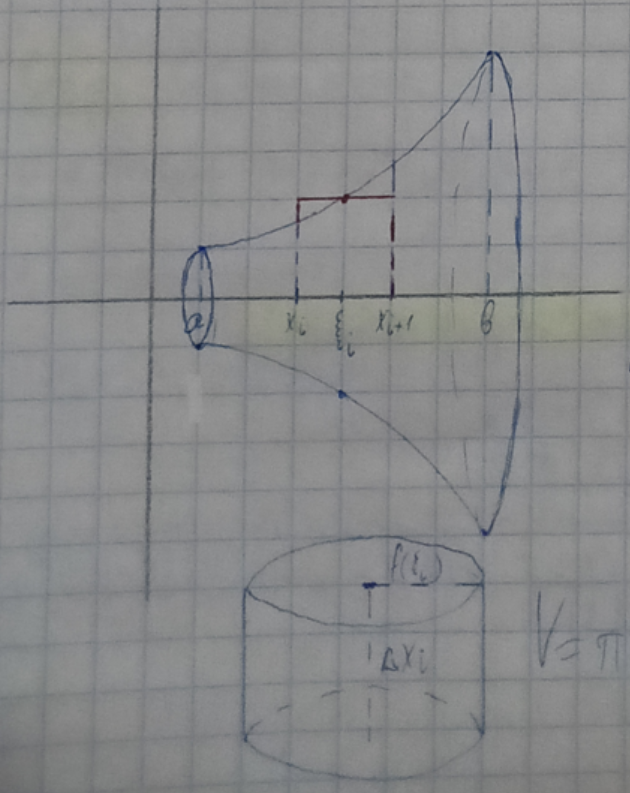
\includegraphics[width=0.7\linewidth]{6.11.1.png}
    \end{center}
    \subsection*{\underline{Если кривая задана в параметрическом виде:}}
    \begin{math}
        \begin{cases}
            x=x(t)\\
            y=y(t)
        \end{cases} \alpha \leq t \leq \beta \; x(\alpha)=a \; x(\beta)=b\\
        V=\pi \int_{a}^{b}f^2(x)dx =
        \begin{vmatrix}
            x=x(t)\\
            dx=x'(t)dt\\
            x=a \Rightarrow t=\alpha\\
            x=a \Rightarrow t=\beta
        \end{vmatrix}=
        \fbox{$\pi \int_{\alpha}^{\beta} y^2(t)x'(t)dt=V_x$}\\
        \fbox{$V_y=\pi \int_{c}^{d} x^2(y)dy=\pi \int_{\alpha_1}^{\beta_1} x^2(t)y'(t)dt$}
    \end{math}
    \subsection*{\underline{Если кривая задана в полярной системе координат:}}
    Пусть $r=r(\phi) \; \alpha \leq \phi \leq \beta$\\
    \begin{math}
        \begin{cases}
            x=rcos(\phi)=r(\phi)cos\phi\\
            y=r(\phi)sin\phi
        \end{cases}\\
        x'(\phi)=r'cos\phi-rsin\phi\\
        \fbox{$V_x=\pi \int_{\alpha}^{\beta} r^2(\phi)sin^2\phi (r'(\phi)cos \phi -r(\phi)sin\phi)d\phi$}\\
        \fbox{$V_y=\pi \int_{\alpha_1}^{\beta_1}r^2(\phi)cos^2(\phi)(r'(\phi)sin\phi + r(\phi)cos\phi)d\phi$}
    \end{math}
    \subsection{Площадь поверхностей тела вращения}
    Пусть f(x) $\geq 0 \; \forall x \in [a;b]\\
    R:a=x_0<x_1<x_2<\dots<x_n=b$\\
    Обозначим $f(a)=M_0,\dots,f(\xi_i)=M_i,\dots,f(b)=M_n$\\
    Соединим (.) $M_i$ ломанными\\
    $\Delta l_i = |M_iM_{i=1}| = \sqrt{1+f'(\xi_i)^2}\Delta x_i \; \Delta x_i$ - произвольная (.)$\in [x_i;x_{i+1}].
    \\P_i=\pi(f(x_{i+1}+f(x_i)))\sqrt{1+f'(\xi_i)^2}\Delta x_i$\\
    Составим $\sigma_R = \sum_{i=0}^{n-1}P_i=\sum_{i=0}^{n-1}\pi(f(x_{i+1}+f(x_i)))\sqrt{1+f'(\xi_i)^2 \Delta x_i}$
    $S_\text{бок} = \pi (R+r)L$\\
    Обозначим $S_\text{бок} = P$.\\
    \begin{center}
        \includegraphics[width=0.5\linewidth]{6.12.1.png}
    \end{center}
    $\sigma_R$ не является интегральной суммой т.к. её значение зависит от $\overset{\underline{x}}{3} (.): \xi_i,x_i,x_{i+1}$
    Рассмотрим $\overline{\sigma_r} = \sum_{i=0}^{n-1} \pi(f(\xi_i)+f(\xi_i))\sqrt{1+f'(\xi_i)^2}\Delta x_i=2\pi \sum_{i=0}^{n-1}f(\xi_i)sqrt{1+f'(\xi_i)^2}\Delta x_i$\\
    $\overline{\sigma_R}$ - интегральная сумма\\
    Можно показать что: $\forall \delta > 0 \exists \varepsilon > 0: \lambda_R<\delta \Rightarrow |\sigma_R-\overline{\sigma_R}|<\varepsilon$\\
    Это значит что $\lim_{\lambda_R \to 0}\sigma_R=\lim_{\lambda_R \to 0}\overline{\sigma_R}$\\
    $\lim_{\lambda_R \to 0} \sigma_R = \lim_{\lambda_R \to 0} \overline{\sigma_R}=2\pi \int_{a}^{b}f(x)\sqrt{1+f'(x)^2}dx=P$\\
    \subsection*{Если функция задана в параметрическом виде:}
    Пусть $\begin{cases}
        x=x(t)\\
        y=y(t)
    \end{cases} \alpha \leq t \leq \beta \; x(\alpha)=a,x(\beta)=b\\
    P_x=\int_{a}^{b}f(x)\sqrt{1+f'(x)^2}dx=\begin{vmatrix}
        x=x(t)\\
        dx=x'(t)dt\\
        x=a \Rightarrow t=\alpha\\
        x=b \Rightarrow t=\beta
    \end{vmatrix}=$\fbox{$2\pi \int_{\alpha}^{\beta}y(t) \underset{dl}{\sqrt{x'(t)^2+y'(t)^2}dt}$}\\
    \fbox{$P_y=\int_{\alpha_1}^{\beta_1}x(t)\sqrt{x'(t)^2+y'(t)^2}dt$}
    \subsection*{Если функция задана в полярной системе координат:}
    Пусть $r=r(\alpha), \alpha \leq \phi \leq \beta$\\
    \fbox{$P_x=2\pi \int_{\alpha}^{\beta}r(\phi)sin(\phi)\sqrt{r^2(\phi)+r'(\phi)^2}d\phi$}\\
    \fbox{$P_x=2\pi \int_{\alpha}^{\beta}r(\phi)cos(\phi)\sqrt{r^2(\phi)+r'(\phi)^2}d\phi$}
    \subsection{Физические приложения определенного интеграла}
    \begin{enumerate}
        \item Вычисление рабочей силы\\
        Пусть (.) движется вдоль оси oX под действием переменной силы F(x). \\Точка перемещается из x=a в x=b перемещается\\
        \begin{enumerate}
            \item R: $a=x_0<x_1<\dots<x_n=b$
            \item Выберем $\xi_i$
            \item Вычислим F($\xi_i$)
            \item Составим $\sigma_R=\sum_{i=0}^{n-1}A_i=\sum_{i=0}^{n-1}F(\xi_i)\Delta x_i$
            $A=\lim_{\lambda_R \to 0}\sigma_R=\int_{a}^{b}F(x)dx$
        \end{enumerate}
        \item Центр тяжести кривой и её моменты относительно осей: рассмотрим f(x) $\geq$ 0 на [a;b]\\
        R:a=$x_0<x_1<\dots<x_n=b$\\
        Будем рассматривать $M_i,M_{i+1}$ - как ломанные, имеющие массу. $\rho =$[кг/м] - линейная плотность\\
        Составим сумму $\sigma_R=\sum_{i=0}^{n-1}f(\xi_i)\rho(\xi_i)\Delta L_i=\sum_{i=0}^{n-1} f(\xi_i)\rho(\xi_i)\sqrt{1+f'(\xi_i)^2}\Delta x_i$\\
        $\lim_{\lambda_R \to 0}\sigma_R=\int_{a}^{b}\underset{r}{f(x)} \underset{m}{\rho\sqrt{1+f'(x)^2}}=M_x$ - момент кривой относительно оси oX\\
        С другой стороны ($x_0,y_0$) - центр тяжести кривой.\\$Mx=my_0$\\
        $my_0=\int_{a}^{b}f(x)\rho\sqrt{1+f'(x^2)}dx;\rho ly_0=\int_{a}^{b}f(x)\rho(x)\sqrt{1+f'(x)^2}dx|пусть \rho = const\\
        ly_0=\int_{a}^{b}f(x)\sqrt{1+f'(x)^2}dx\\
        l2\pi y_0=2 \pi \int_{a}^{b} f(x)\sqrt{1+f'(x)^2}dx$\\
        \subsubsection*{Теорема 6.13.1  1-ая Теорема Гульдена}\label{th:6.13.1}
        Площадь поверхности, полученной вращением кривой относительно оси oX, равна длине этой кривой, умноженной на длину окружности, которую описывает центр тяжести вокруг оси oX.\par\noindent
        \underline{Доказательство:}
        \begin{adjustwidth}{1.5em}{1.5em}
            См. выше\\
            $\begin{cases}
                x_0=\frac{M_y}{m}\\
                y_0=\frac{M_x}{m}
            \end{cases} =
            \begin{cases}
                x_0=\frac{\int_{a}^{b}x\rho (x)\sqrt{1+f'(x)^2}dx}{\int_{a}^{b}\underset{\rho}{\rho (x)}\underset{dl}{\sqrt{1+f'(x)^2}dx}dx}\\
                y_0=\frac{\int_{a}^{b}y\rho (x)\sqrt{1+f'(x)^2}dx}{\int_{a}^{b}\rho (x)\sqrt{1+f'(x)^2}dx}
            \end{cases}$
        \end{adjustwidth}
        \item Центр тяжести плоской фигуры и её момент относительно осей:\\
        Пусть $f(x)\geq 0,g(x)\geq 0. \forall x \in [a;b]$
        Пусть $0 \leq g(x) \leq f(x)\\
        R:a=x_0<x_1<\dots<x_n=b$\\
        Выберем произвольно (.) $\xi_i\in [x_i,x_{i+1}]. \rho(\xi_i)=const$\\
        Составим $\sigma_R$\\
        $\sigma_R=\sum_{i=0}^{n-1}\frac{1}{2} \underset{r_x}{[f[\xi_i]+g(\xi_i)]}\rho(\xi_i)\overset{\text{высота}}{[f(\xi_i)-g(\xi_i)]}\overset{\text{ширина}}{\Delta x_i}$\\
        $[\rho]-\frac{\text{кг}}{\text{м}^2} - $поверхностная плотность\\
        $\lim_{\lambda_R \to 0} = \int_{R}^{b}\frac{1}{2}\rho (x) [f^2(x)-g^2(x)]dx=M_x$\\
        С другой стороны $M_x=my_0(y_0$ - у координата центра тяжести)\\
        \begin{math}
            my_0=\int_{a}^{b}\frac{1}{2}\rho (x)[f^2(x)-g^2(x)]dx\\
            \rho Sy_0=\int_{a}^{b}\frac{1}{2}\rho (x)[f^2(x)-g^2(x)]dx|:\rho=const|*2\pi\\
            S*2\pi y_0=\pi \int_{a}^{b} [f^2(x)-g^2(x)]dx\\
        \end{math}
        \subsubsection*{Теорема 6.13.2 2-ая Теорема Гульдена}\label{th:6.13.2}
        Объём тела, полученного вращением плоской фигуры вокруг оси oX, равен площади этой фигуры, умноженной на длину окружности, которую описывает центр тяжести вокруг оси oX.\par\noindent
        $\begin{cases}
            y_0=\frac{M_x}{m}=\frac{\frac{1}{2}\int_{a}^{b}\rho (x)[f^2(x)-g^2(x)]dx}{\int_{a}^{b}\rho(x)[f(x)-g(x)]dx}\\
            x_0=\frac{M_y}{m}=\frac{\int_{a}^{b}x\rho (x)[f(x)-g(x)]dx}{\int_{a}^{b}\rho (x)[f(x)-g(x)]dx}
        \end{cases}$
    \end{enumerate}
    \subsection{Несобственные интегралы I рода}
    \underline{Определение: } Пусть f(x) задана на конечном [a;b)\\
    Допустим что f(x) интегрируема на [a;b'],b'<b и неограниченна в (.) x=b. Тогда f(x) не интегрируема по Риману на [a;b] \\
    Если существует конечный $\lim_{b' \to b} \int_{a}^{b'}f(x)dx,$ то он называется несобственным интегралом от f(x) на [a;b]\\
    $\int_{a}^{b}f(x)dx=\lim_{b' \to b}\int_{a}^{b'} f(x)dx$\\
    \underline{Определение: } Если b=$\inf$, т.е. f(x) задана на [a;$+ \infty]$ и интегрируема на $\forall [a;A],a<A<\infty$ и существует конечный
    $\lim_{A \to \inf}\int_{a}^{A} f(x)dx,$ то он называется несобственным интегралом 1-рода от функции f(x) на [a;$+\infty$]\\
    Аналогично, $\int_{-\infty}^{b}f(x)dx=\lim_{B \to -\infty} \int_{B}^{b}f(x)dx\\
    \int_{-\infty}^{\infty} f(x)dx=\int_{-\infty}^{C}f(x)dx+\int_{C}^{+\infty}f(x)dx$
    \subsection{Несобственные интегралы 2-го рода}
    \underline{Определение: } Пусть f(x) непрерывна $\forall x \in [a;b]/c \; a \leq c \leq b$\\
    Тогда $\int_{a}^{b}f(x)dx=\int_{a}^{c} f(x)dx+\int_{c}^{b} f(x)dx=\lim_{\varepsilon \to 0}\int_{a}^{c-\varepsilon}f(x)dx+\lim_{\varepsilon \to 0}\int_{c+\varepsilon}^{b}f(x)dx$\\
    Если оба предела существуют то интеграл сходится.\\
    Если хотя бы один не существует или $\pm \infty$, то расходится.\\
    \underline{Замечание:} (.) C может быть c=a или c=b\\
    \underline{Замечание:} Можно записать в виде $\int_{a}^{b}f(x)dx=\lim_{x \to c-0}\int_{a}^{c}f(x)dx+\lim_{x \to c+0} \int_{c}^{b}f(x)dx$\\
    \underline{Пример:}\\
    \begin{enumerate}
        \item Рассмотрим $\int_{1}^{\infty}\frac{dx}{x^k}$
        \begin{enumerate}
            \item k=1. $\int_{1}^{\infty}\frac{dx}{x}=\lim_{A \to \infty}\int_{1}^{A} \frac{dx}{x}=\lim_{A \to \infty} ln |x|\Big|^A_1 = \lim_{A \to \infty}(ln |A|-ln1)=\infty$ - рсх.
            \item k $\ne, k \geq 0 \; \int_{1}^{\infty} \frac{dx}{x^k}=\lim_{A \to \infty}\int_{1}^{A} \frac{dx}{x^k}=\lim_{A \to \infty} (\frac{x^{-k+1}}{-k+1}\Big|^A_1)=\lim_{A \to \infty}
            (\frac{A^{1-k}}{1-k}-\frac{1}{1-k})=\begin{cases}
                \infty,0\leq k<1 \text{-рсх}\\
                \frac{1}{k-1},k>1\text{-сх}
            \end{cases} \int_{1}^{\infty}\frac{dx}{x^k}=\begin{cases}
                \text{сх при k>1}\\
                \text{рсх при k$\leq 1$}
            \end{cases}$
        \end{enumerate}
        \item $\int_{0}^{1} \frac{dx}{x^k} \; \varepsilon>0$
        \begin{enumerate}
            \item k=1, $\int_{0}^{1} \frac{dx}{x}=\lim_{\varepsilon \to 0}\int_{0+\varepsilon}^{1}\frac{dx}{x}=\lim_{\varepsilon \to 0}ln|x|\Big|^1_\varepsilon =\lim_{\varepsilon \to 0}(ln1-ln|\varepsilon|)=+\infty$ - рсх
            \item $k\ne 1, \int_{0}^{1} \frac{dx}{x^k} = \lim_{\varepsilon \to 0}\int_{\varepsilon}^{1}\frac{dx}{x^k}=\lim_{\varepsilon \to 0}\frac{x^{-k+1}}{-k+1}\Big|^1_\varepsilon =\lim_{\varepsilon \to 0}
            (\frac{1}{1-k}-\frac{\varepsilon^{1-k}}{1-k})=\begin{cases}
                \frac{1}{1-k},k<1\\
                \infty,k>1
            \end{cases} \\\int_{0}^{1}\frac{dx}{x^k}=\begin{cases}
                \frac{1}{1-k},k<1\\
                \text{рсх}, k\geq 1
            \end{cases}$
        \end{enumerate}
    \end{enumerate}
    \subsection{Свойство несобственных интегралов}
    \underline{Замечание:} в (.) x=b - особенность
    \begin{enumerate}
        \item Линейность\\
        Если $\int_{a}^{b}f(x)dx и \int_{a}^{b} g(x)dx$ сходятся, то $\int_{a}^{b} [\lambda f(x)+\mu g(x)]dx$ тоже сходятся\\
        $\int_{a}^{b}[\lambda f(x)+\mu g(x)]dx=\lambda \int_{a}^{b} f(x)dx + \mu \int_{a}^{b}g(x)dx$\\
        \underline{Доказательство:}
        \begin{adjustwidth}{1.5em}{1.5em}
            Рассмотрми $\int_{a}^{b}[\lambda f(x)+\mu g(x)]dx=\lim_{b' \to b} \int_{a}^{b}[\lambda f(x)+\mu g(x)]dx= \\ \lim_{b' \to b}[\lambda \int_{a}^{b'}f(x)dx+\mu \int_{a}^{b'}g(x)dx]=
            \lambda\lim_{b' \to b} \int_{a}^{b'}f(x)dx+\mu\lim_{b' \to b}\int_{a}^{b'}g(x)dx=\\ \lambda \int_{a}^{b}f(x)dx+\mu \int_{a}^{b}g(x)dx$
            \begin{center}
                \textbf{Ч.т.д.}
            \end{center}
        \end{adjustwidth}
        \item Если $\int_{a}^{b} f(x)dx$ и $\int_{a}^{b} g(x)dx$ сходятся и $\forall x \in [a;b) f(x) \leq g(x), $ то $\int_{a}^{b}f(x)dx \leq \int_{a}^{b}g(x)dx$\\
        \underline{Доказательство:}
        \begin{adjustwidth}{1.5em}{1.5em}
            $\forall b<b' \; \int_{a}^{b'} f(x) \leq \int_{a}^{b'} g(x)dx$(оценки интервалов)\\
            Переходя к $\lim_{b' \to b}$ при $b' \to b$, получим
            \begin{center}
                \textbf{Ч.т.д.}
            \end{center}
        \end{adjustwidth}
        \item Формула замены переменной\\
        Если f(x) непрерывна $\forall x \in [a;b) = \Delta x$\\
        $\phi(t)$ непрерывно дифференцируема на [$\alpha;\underset{\Delta t}{\beta})(\phi(t)$ непрерывна и $\phi'(t)$ непрерывна)\\
        $\phi(\Delta t) \subset \Delta x,a=\phi(\alpha),b=\lim_{t \to \beta}\phi(t)$\\
        Тогда $\int_{a}^{b}f(x)dx=\int_{\alpha}^{\beta} f(\phi(t))\phi'(t)dt$
        \item Формула интегрирования по частям\\
        Если u(x) и v(x) непрерывна на [a;b), u'(x),v'(x) конечно-непрерывна на [a;b'] a<b'<b, \\ то $\int_{a}^{b}udv=uv\Big|^b_a - \int_{a}^{b}vdu$\\
        $\int_{a}^{b}udv=\lim_{b' \to b} (u(b')v(b')-u(a)v(a)-\int_{a}^{b'}vdu)$
    \end{enumerate}
    \underline{Пример:}\\

    \[\int_{1}^{\infty}\frac{dx}{x\sqrt{x^2-1}}=\lim_{\substack{A \to \infty \\ \varepsilon \to 0}} \int_{1+\varepsilon}^{A} \frac{dx}{x\sqrt{x^2-1}} =
    \begin{vmatrix}
        x=\frac{1}{t} & x=1 \Rightarrow t=1\\
        dx=-\frac{1}{t^2}dt & x=\infty \Rightarrow t=0
    \end{vmatrix} = \int_{1}^{0} \frac{-\frac{dt}{t^2}}{\frac{1}{t}\sqrt{\frac{1}{t^2}-1}}=\int_{0}^{1}\frac{dt}{t\sqrt{\frac{1-t^2}{t^2}}}=\] \\
    \[\int_{0}^{1} \frac{dt}{t\sqrt{\frac{1-t^2}{t^2}}}=
    \int_{0}^{1}\frac{dt}{\sqrt{1-t^2}}=\lim_{\varepsilon \to 0} \int_{0}^{1-\varepsilon}\frac{dt}{\sqrt{1-t^2}}=\lim_{\varepsilon \to 0} arcsin t\Big|^{1-\varepsilon}_0=\\
    \lim_{\varepsilon \to 0}[arcsin(1-\varepsilon)-arcsin(0)]=\frac{\pi}{2} \] \\
    \subsection{Несобственные интегралы от неотрицательных функций}
    \textbf{Лемма :} Если f(x) неотрицательна на [a;b), то для сходимости $\int_{a}^{b}f(x)dx \longleftrightarrow $ чтобы множество
    интегралов $\int_{a}^{b'} f(x)dx \; b' \in [a;b)$ было ограничено сверху. Т.е. чтобы $\exists c>0:\forall b':\int_{a}^{b'}f(x)dx \leq C$\\
    \underline{Доказательство:}
    \begin{adjustwidth}{1.5em}{1.5em}
        Рассмотрим $\phi(b') = \int_{a}^{b'} f(x)dx - $ функия с переменным верхним пределом.\\
        Пусть a<b'<b''<b\\
        Рассмотрим $\phi(b'')=\int_{a}^{b''}f(x)dx = \int_{a}^{b'}f(x)dx+\int_{b'}^{b''}f(x)dx\geq \int_{a}^{b'}f(x)dx=\phi(b'),$ Т.е. если $b'<b'' \Rightarrow
        \phi(b')\leq \phi(b'').$ Т.е. $\phi(b') $ неубывающая функция.\\
        Существование $\int_{a}^{b}f(x)dx$ означает по определению существование конечного предела $\lim_{b' \to b}\phi(b')=\int_{a}^{b}f(x)dx,$ который существует $\longleftrightarrow$ когда $\phi(b')$
        ограничена сверху, Т.е. $\phi(b') \leq C.$
    \end{adjustwidth}
    \begin{center}
        \textbf{Ч.т.д.}
    \end{center}
    \subsubsection*{Теорема 6.17.1 Признак сравнения несобственных интегралов (Первый признак)}\label{th:6.17.1}
    Пусть $0\leq g(x) \leq f(x). x\in [a;b)$\par\noindent
    Тогда \begin{enumerate}
        \item Если $\int_{a}^{b}f(x)dx$ сх $\Rightarrow \int_{a}^{b}g(x)dx$ сх
        \item Если $\int_{a}^{b}g(x)dx$ рсх $\Rightarrow \int_{a}^{b}f(x)dx$ рсх 
    \end{enumerate}
    \underline{Доказательство:}
    \begin{adjustwidth}{1.5em}{1.5em}
        \begin{enumerate}
            \item Пусть $\int_{a}^{b}f(x)dx $ сх, тогда множество интегралов $\int_{a}^{b'}f(x)dx$ по лемме ограничены сверху.
            Т.к. $g(x) \leq f(x) \Rightarrow \int_{a}^{b'}g(x)dx \leq \int_{a}^{b'}f(x)dx \Rightarrow \forall b' \in (a;b)$ множество интегралов $\int_{a}^{b'}
            g(x)dx$ будут ограничены сверху. $\Rightarrow$ по лемме $\int_{a}^{b}g(x)dx$ сх.
            \item Пусть $\int_{a}^{b}g(x)dx$ рсх, тогда $\int_{a}^{b}f(x)dx$ не может сходится,т.к. если бы они сх, то $\int_{a}^{b}g(x)dx$ тоже сх по п.1, а это не так.
        \end{enumerate}
        \begin{center}
            \textbf{Ч.т.д.}
        \end{center}
    \end{adjustwidth}
    \subsubsection*{Теорема 6.17.2 Следствие признака сравнения (Второй признак сравнения)}\label{th:}
    Пусть $\forall x \in [a;b) f(x)\geq 0,g(x)\geq 0$ и $\lim_{x \to b}\frac{f(x)}{g(x)}=k$\par\noindent
    \begin{enumerate}
        \item Если $\int_{a}^{b}g(x)dx$ - сх. $0\leq k< \infty$ - конечные $\Rightarrow \int_{a}^{b}f(x)dx$ сх.
        \item Если $\int_{a}^{b}g(x)dx$ - рсх. $0<k\leq \infty \Rightarrow \int_{a}^{b}f(x)dx$ - рсх.
    \end{enumerate}
    \underline{Доказательство:}
    \begin{adjustwidth}{1.5em}{1.5em}
        \begin{enumerate}
            \item Пусть $0\leq k < \infty$\\
            Т.К. $\lim_{x \to b} \frac{f(x)}{g(x)} = k$, то $\exists b' \in [a;b):\forall x\in (b';b) \frac{f(x)}{g(x)}<{k+1}$\\
            $\int_{a}^{b}g(x)dx - $сх $\Rightarrow \int_{b}^{b}g(x)dx$ сх $\Rightarrow \int_{b'}^{b}(k+1)g(x)dx$ сх $\Rightarrow \int_{b'}^{b}f(x)dx$ сх 
            по признаку сравнения $\Rightarrow \int_{a}^{b}f(x)dx$сх.
            \item Пусть $0<k\leq \infty$. Пусть $0<k'<k$.\\
            $\int_{a}^{b}g(x)dx$ - рсх. Тогда $\forall x \in (b';b) \frac{f(x)}{g(x)}>k'$\\
            f(x)>k'g(x)\\
            $\int_{a}^{b}g(x)dx$ рсх. $\Rightarrow \int_{b'}^{b} g(x)dx$ рсх. $\Rightarrow \int_{b'}^{b} k'g(x)dx$ рсх. $\Rightarrow \int_{b'}^{b}f(x)dx$ по признаку
            сравнения $\Rightarrow \int_{a}^{b}f(x)dx$ рсх. 
            \begin{center}
                \textbf{Ч.т.д.}
            \end{center}
        \end{enumerate}
    \end{adjustwidth}
    \underline{Пример:}  $\int_{0}^{1} ln(x)dx$\\
    Пусть f(x)=ln(x)\\
    $g(x)=\frac{1}{x^2} \; \int_{0}^{1}\frac{dx}{x^2}$ - рсх.\\
    $\lim_{x \to 0}\frac{ln(x)}{\frac{1}{x^2}}=\lim_{x \to 0}\frac{\frac{1}{x}}{-\frac{2}{x^3}}=\lim_{x \to 0}\frac{x^2}{-2}=0$\\
    $g(x)=\frac{1}{\sqrt{x}} \; \int_{0}^{1}=\frac{dx}{\sqrt{x}}-$ сх.\\
    Рассмотрим $\lim_{x \to 0}\frac{ln(x)}{\frac{1}{\sqrt{x}}}=\lim_{x \to 0}\frac{\frac{1}{x}}{-\frac{1}{2x^{\frac{3}{2}}}}=\lim_{x \to 0}(-2\sqrt{x})=0
    \Rightarrow \int_{0}^{1}ln(x)dx$- сх.
    \subsection{Критерий Коши сходимсоти несобственных интегралов. Абсолютно сходящиеся интегралы.}
    \subsubsection*{Теорема 6.18.1}\label{th:6.18.1}
    $\int_{a}^{b}f(x)dx$ сх $\Longleftrightarrow$ когда $\forall \varepsilon > 0 \exists a<b_0<b:\forall b',b'':b_0<b'<b''<b$\par\noindent
    $\Big| \int_{b'}^{b''}f(x)dx \Big| < \varepsilon$
    \underline{Доказательство:}
    \begin{adjustwidth}{1.5em}{1.5em}
        Рассмотрим $\phi(b_0)=\int_{a}^{b_0}f(x)dx$ - функция с переменным верхним пределом.\\
        Существование $\int_{a}^{b}f(x)dx$ означает существование $\lim_{b_0 \to b}\phi(b_0)$\\
        $\lim_{b_0 \to b}\phi(b_0) \exists \Longleftrightarrow$ когда $\exists$ окружность (.) b: $\forall b',b'' \in $ окружности: $|b''-b'|<\delta \Rightarrow |\phi(b'')-\phi(b')|<\varepsilon$\\
        А это означает $\Big| \int_{a}^{b''}f(x)dx - \int_{a}^{b'}f(x)dx \Big| < \varepsilon \Rightarrow \Big| \int_{b'}^{b''} f(x)dx \Big| < \varepsilon$
    \end{adjustwidth}
    \begin{center}
        \textbf{Ч.т.д.}
    \end{center}
    \underline{Определение: } Пусть f(x) задана на [a;b) и интегрируема по Риману $\forall [a;b'] a<b'<b$\\
    $\int_{a}^{b}f(x)dx$ называется пбсолютно сходящимися, если сходятся $\int_{a}^{b}|f(x)|dx$
    \subsubsection*{Теорема 6.18.2 Критерий Коши абсолютной сходимости несобственных интегралов}\label{th:6.18.2}
    Для того, чтобы $\int_{a}^{b}f(x)dx$ абсолютно сх $\Longleftrightarrow \forall \varepsilon >0 \exists b_0:a<b_0<b: \forall b',b'':\\b_0<b'<b''<b \Rightarrow |\int_{b'}^{b''}|f(x)dx|| < \varepsilon$\par\noindent
    \underline{Доказательство:}
    \begin{adjustwidth}{1.5em}{1.5em}
        следует из критерия Коши для интеграла $\int_{a}^{b}|f(x)|dx$
    \end{adjustwidth}
    \begin{center}
        \textbf{Ч.т.д.}
    \end{center}
    \subsubsection*{Теорема 18.3}\label{th:6.18.3}
    Если несобственный интеграл абсолютно сходится, то он сходится.\par\noindent
    \underline{Доказательство:}
    \begin{adjustwidth}{1.5em}{1.5em}
        $\int_{a}^{b}|f(x)|dx$ сх, тогда по критерию Коши на (a;b) $\exists b_0:b_0<b'<b''<b \Rightarrow |\int_{b'}^{b''}|f(x)|dx|< \varepsilon$\\
        Рассмотрим $|\int_{b'}^{b''}f(x)dx|\leq |\int_{b'}^{b''}|f(x)|dx|<\varepsilon,$ Т.е. выполняется критерий Коши сходимости интеграла $\int_{a}^{b}f(x)dx$
    \end{adjustwidth}
    \begin{center}
        \textbf{Ч.т.д.}
    \end{center}
    \underline{Свойство: } Если $\int_{a}^{b}f(x)dx$ абсолютно сходится\\
    g(x) интегируема по Риману $\forall [a;b'] \subset [a;b)$ и ограничена на [a;b), то $\int_{a}^{b}f(x)g(x)dx$ сх.\\
    \underline{Доказательство:}
    \begin{adjustwidth}{1.5em}{1.5em}
        $\int_{a}^{b'}f(x)dx \exists $ по условию, $\int_{a}^{b'}g(x)dx \exists$ по условию $\Rightarrow \int_{a}^{b'}f(x)g(x)dx \exists$(по свойству)\\
        Рассмотрим $\int_{a}^{b}|f(x)g(x)|dx \leq \underset{\text{абсолютная сх по условию}}{c\int_{a}^{b}|f(x)|dx}$\\
        Тогда $\int_{a}^{b}|f(x)g(x)|dx$ сх, по 1-му признаку сравнения.\\
        Тогда $\int_{a}^{b}f(x)g(x)dx$ сх. абсолютно по Опр.
    \end{adjustwidth}
    \begin{center}
        \textbf{Ч.т.д.}
    \end{center}
    \subsection{Признаки сходимости Дирихле́ и Абеля несобственных интегралов 1-го рода}
    \subsubsection*{Теорема 6.19.1 Признак Дирихле́}\label{th:6.19.1}
    Если на полуоси $x\geq a$\par\noindent
    \begin{enumerate}
        \item f(x) непрерывна и имеет ограниченную первообразную на $x\geq a$
        \item g(x) непрерывно дифференцируема и убывает при этом $\lim_{x \to \infty}g(x)=0$
    \end{enumerate}
    Тогда $\int_{a}^{\infty}f(x)g(x)dx$ сх.\\
    \underline{Доказательство:}
    \begin{adjustwidth}{1.5em}{1.5em}
        Пусть F(x) - ограниченная первообразная f(x) на $x \geq a$\\
        Рассмотрим $\int_{a}^{b}f(x)g(x)dx=\int_{a}^{b}\underset{u}{g(x)} \underset{du}{d(F(x))}=g(x)F(x)\Big|^b_a-\int_{a}^{b}F(x)g'(x)dx=
        g(b)F(b)-g(a)F(a)-\int_{a}^{b}F(x)g'(x)dx$\\
        Рассмотрим $\lim_{b \to \infty}\underset{\rightarrow 0}{g(b)} \underset{\rightarrow \text{огр.}}{F(b)}=0.$ Докажем что $\int_{a}^{\infty}F(x)g'(x)dx$ сх.\\
        Рассмотрим $\int_{a}^{b}|F(x)g'(x)|dx=-\int_{a}^{b}|F(x)|g'(x)dx \leq -c \int_{a}^{b}g'(x)dx=-c g(x)\Big|^b_a=\\c(g(a)-g(b))\leq cg(a)-const$
        Получим что множество интегралов $\int_{a}^{b}|F(x)g'(x)|dx$ ограничены сверху $\Rightarrow \int_{a}^{\infty}|F(x)g'(x)|dx$ сх(по Лемме \S 17)
        $\Rightarrow \int_{a}^{\infty}F(x)g'(x)dx$ абсолютно сходится по опрделению $\Rightarrow$ сх.(\hyperref[th:6.18.3]{Th. 6.18.3})\\
        Тогда $\int_{a}^{\infty}f(x)g(x)dx$ сходятся. 
    \end{adjustwidth}
    \begin{center}
        \textbf{Ч.т.д.}
    \end{center}
    \subsubsection*{Теорема 6.19.2 Признак Абеля}\label{th:6.19.2}
    Если на $x\geq a$\par\noindent
    \begin{enumerate}
        \item f(x) непрерывна на $x \geq a$ и $\int_{a}^{\infty}f(x)dx$ сх.
        \item g(x) непрерывно дифференцируема, ограниченна и монотонна.
    \end{enumerate}
    Тогда $\int_{a}^{\infty}f(x)g(x)dx$ сх.\\
    \underline{Доказательство:}
    \begin{adjustwidth}{1.5em}{1.5em}
        \underline{Замечание:} $\int_{a}^{\infty}f(x)g(x)dx$ и $\int_{a}^{\infty}f(x)(-g(x))dx$ сх. или рсх. одновременно.\\
        Тогда одна из функция g(x) или (-g(x)) будет убывающей(невозрастающей).\\
        Пусть для определённости g(x) убывает.\\
        По условию $\lim_{x \to \infty}g(x)=C$\\
        Т.е. $\lim_{x \to \infty}(g(x)-C)=0$\\
        Рассмотрим f(x)g(x) = f(x)g(x)-cf(x)+cf(x)=f(x)[g(x)-c]+cf(x)\\
        Надо показать что $\int_{a}^{\infty}f(x)[g(x)-c]dx$ сх. и $\int_{a}^{\infty}cf(x)dx$ сх.\\
        $c\int_{a}^{\infty}f(x)dx$ сх. по условию.\\
        Рассмотрим $\int_{a}^{\infty}f(x)dx=\int_{a}^{\infty}f(t)dt=\lim_{x \to \infty}\int_{a}^{x}f(t)dt=
        \lim_{x \to \infty}F(x); \int_{a}^{\infty}f(x)dx$ сх.  $\Rightarrow \lim_{x \to \infty}F(x) \exists \Rightarrow F(x)$ ограничена в окржуности бесконечно удалённой точки.\\
        F(x) первообразная для f(x) на $x \leq a$\\
        Рассмотрим $\int_{a}^{\infty}f(x)[g(x)-c]dx.$ Тогда интеграл сходится по признаку Дирихле́, Т.е. $\int_{a}^{\infty}f(x)g(x)dx$ сх.\\
    \end{adjustwidth}
    \begin{center}
        \textbf{Ч.т.д.}
    \end{center}
    \underline{Примеры:}\\
    \begin{enumerate}
        \item $\int_{1}^{\infty}\frac{sin(x)}{x^\alpha}dx \; \alpha>0$\\
        f(x) = sin(x)(непр. имеет огр. перв.) \; g(x)=$\frac{1}{x^\alpha}$(непрерывно диф-ма $\lim_{x \to \infty}\frac{1}{x^\alpha}=0$, убывает)\\
        Интеграл сходится по признаку Дирихле́
        \item $\int_{1}^{\infty}\frac{sin(x)arctg(x)}{x^\alpha}dx \; \alpha>0$\\
        $f(x)=\frac{sin(x)}{x^\alpha}$(непр. и $\int_{1}^{\infty}\frac{sin(x)}{x^\alpha}$ сх.) \; g(x)=arctg(x)(непр. дифф-ма,огр. возрастает)\\
        Тогда $\int_{1}^{\infty}\frac{sin(x)arctg(x)}{x^\alpha}dx$ сх. по признаку Абеля.
    \end{enumerate}

    \section{Функции нескольких переменных}
    \subsection{Основные понятия}
    Рассмотрим упорядоченное множество $E$ пар чисел $(x; y)$\\
    Пары $(x_1; y_1)$ и $(x_2; y_2)$ равны $\Leftrightarrow$ $x_1 = x_2, y_1 = y_2$.\par\noindent
    Пусть каждой паре $(x; y) \in E$ по некоторому закону ставится в соответствие единственное число $z$. Тогда говорят, что на $E$ определена функция $z = f(x; y)$.\\
    \underline{Примеры:}
    \begin{center}
        \includegraphics{7.1.1.png}
    \end{center}
    Рассмотрим множество упорядоченных систем
    \[ (x_1, x_2, \dots, x_n), n \in N \]
    Элементы этого множества можно рассматривать как точку $n$-мерного пространства $R^n$, а можно как $n$-мерные векторы.\\
    В первом случае для них вводится понятие расстояния, во втором случае - соответствующие векторные операции.\par\noindent
    \textbf{В случае вектора:}
    \begin{align*}
        \text{Пусть }&\overline{x} (x_1, \dots, x_n)\\
        &\overline{y}(y_1,\dots,y_n)
    \end{align*}
    \begin{gather*}
        \lambda\overline{x} + \mu \overline{y} = (\lambda x_1 + \mu y_1; \lambda x_2 + \mu y_2; \dots; \lambda x_n + \mu y_n)\\
        \overline{x}\overline{y} = x_1y_1 + \dots + x_ny_n
    \end{gather*}
    Множество всех упорядоченных систем $\overline{x} = (x_1, \dots, x_n)$, для которых определены линейная комбинация и скалярное произведение двух элементов называется $n$-мерным арифметическим Евклидовым пространством.\par\noindent
    \textbf{В случае точки:}
    \begin{gather*}
        \rho (x,y) \text{ - расстояние между точками}\\
        \rho (x,y) = |x - y| = \sqrt{ \sum_{i = 1}^{n} (x_i - y_i)^2 }
    \end{gather*}
    Множество точек $x = (x_1, \dots, x_n)$, для которых выполняется неравенство $\rho (x, x^0) < \varepsilon$, называется $\varepsilon$-окрестностью точки $x^0$.\\
    Точки множества называется внутренними точками, если $\exists$ $\varepsilon$-окрестность, целиком содержащаяся в этом множестве.\\
    Точки множества называется граничными точками, если $\forall$ её $\varepsilon$-окрестность содержит как внутренние, так и внешние точки.\\
    Точки множества называется внешними точками, если $\exists$ $\varepsilon$-окрестность, не содержащая ни одной точки множества.\par\noindent
    Пусть в $R^n$
    \begin{center}
        \includegraphics{7.1.2.png}
    \end{center}
    Т.е. в пространстве $R^n$ задана последовательность $\{x^k\}$.\\
    Точка $x^0 = (x^0_1, x^0_2, x^0_3, \dots, x^0_n)$ называется пределом последовательности $\{x^k\}$, если $\lim_{k\to\infty} \rho(x^k, x^0) = 0$\\
    Обозначение: $\lim_{k\to\infty}x^k=x^0$\\
    Или: Точка $x^0 = (x^0_1, x^0_2, x^0_3, \dots, x^0_n)$ называется пределом последовательности $\{x^k\}$, если $\forall \varepsilon > 0$ $\exists \text{ } n_0 \text{ } \big| \text{ } \forall n > n_0 : \rho(x^n, x^0) < \varepsilon$\\
    Определение $\lim_{k\to\infty}x^k=x^0$ эквивалентно $n$ одномерным пределам.
    \[ \lim_{k\to\infty}x^k_1 = x^0_1; \lim_{k\to\infty}x^k_2 = x^0_2; \dots; \lim_{k\to\infty}x^k_n = x^0_n \]

    \subsection{Предел функций нескольких переменных в точке}
    \noindent Пусть функция $f(x_1, \dots, x_n)$ определена в $u(x^0)$, быть может за исключением самой точки $x^0$.\\
    \textbf{По Гейне:} точка $a$ (одномерное число) называется пределом функции $f$ в точке $x^0$ ($f(x_1, \dots, x_n)$), если $\forall$ последовательности $\{x^k\} : \lim_{k\to\infty}x^k=x^0$, числовая последовательность $\{ f(x^k) \}$ (одномерная) имеет своим пределом точку $a$ ($\lim_{k\to x^0}f(x)=a$).\par\noindent
    \textbf{По Коши:} точка $a$ называется пределом функции $f(x_1, \dots, x_n)$ в точке $x^0$, если
    \[ \forall \varepsilon > 0 \text{ } \exists \text{ } \delta = \delta(\varepsilon) > 0 : \rho(x, x^0) < \delta \implies |f(x_1, \dots, x_n) - a| < \varepsilon \]
    Рассмотрим функцию $f(x,y)$, заданную в окрестности точки $(x_0; y_0)$
    \begin{adjustwidth}{1.5em}{1.5em}
        Пусть $\overline{\omega} (\omega_x, \omega_y)$ - единичный вектор.\\
        $\frac{x - x_0}{\omega_x} = \frac{y - y_0}{\omega_y}$ - уравнение прямой, проходящей через точку $(x_0; y_0)$ с направляющим вектором $\overline{\omega}$.
        \[ \begin{cases}
            x = \omega_xt + x_0\\
            y = \omega_yt + y_0
        \end{cases}\text{ - параметрическое уравнение прямой} \]
        Пусть $t \ge 0$. Получим луч, выходящий из точки $(x_0; y_0)$ в направлении $\overline{\omega}$.
        \begin{center}
            \includegraphics{7.2.1.png}
        \end{center}
        Рассмотрим $\underbrace{f(x; y)}_{\text{ф. 2-х перем. x, y}} = \underbrace{f(x_0+\omega_xt; y_0+\omega_yt)}_{\text{ф. 1 перем. t}}$.
    \end{adjustwidth}
    $\lim_{t \to 0} f(x_0+\omega_xt; y_0+\omega_yt)$, если он $\exists$, называется пределом функции $f(x, y)$ в точке $(x_0; y_0)$ по направлению $\overline{\omega}$.\\
    \underline{Пример:}
    \begin{adjustwidth}{1.5em}{1.5em}
        Рассмотрим $f(x,y) = \frac{x^2y}{x^4 + y^2}$; $f(x,y)$ определена $\forall x, y \in R$, кроме точки $(0, 0)$.
        \[ \lim_{x \to 0\,y \to 0} \frac{x^2y}{x^4 + y^2} = \left[ \frac{0}{0} \right] = \begin{vmatrix}
            y = kx\\
            x \to 0 \Rightarrow y \to 0
        \end{vmatrix} = \lim_{x\to 0} \frac{kx^3}{x^4+k^2x^2} = \lim_{x \to 0}\frac{kx}{x^2+k^2} = 0 \]
        Проверим, может ли быть несовпадение пределов при другом значении $y$.
        \[ \lim_{x \to 0\,y \to 0} \frac{x^2y}{x^4 + y^2} = \begin{vmatrix}
            y = x^2\\
            x \to 0 \Rightarrow y \to 0
        \end{vmatrix} = \lim_{x \to 0}\frac{x^4}{x^4+x^4} = \frac{1}{2} \]
        Пределы не совпали $\Rightarrow$ предел $\nexists$.
    \end{adjustwidth}
    Определение:
    \[\begin{matrix}
        \lim_{x \to x_0\, y \to y_0}f(x;y)=\infty & \forall M > 0\, \exists\, \delta = \delta(M): \rho(\underset{M(x,y)}{M}, \underset{M_0(x_0, y_0)}{M_0}) < \delta \Rightarrow |f(x;y)| > M\\
        \lim_{x\to\infty\, y\to\infty}f(x,y) = a & \forall \varepsilon > 0\, \exists\, K = K(\varepsilon): |x| > K, |y| > K \Rightarrow |f(x,y) - a| < \varepsilon\\
        \lim_{x\to-\infty\, y\to y_0}f(x,y) = -\infty & \forall M > 0\, \exists\, \delta = \delta(M): x < -\frac{1}{\delta}, |y-y_0|<\delta \Rightarrow f(x,y) < -M
    \end{matrix}\]

    \subsection{Непрерывность функций нескольких переменных.}
    Функция $f(x_1, \dots, x_n)$ называется непрерывной в точке $x^0 = (x^0_1, x^0_2, \dots, x^0_n)$, если она определена в некоторой окрестности точки $x^0$, в том числе и в самой точке $x^0$ и $\lim_{x \to x_0} f(x) = f(x^0)$ при $x = (x_1, \dots, x_n)$, $x^0 = (x^0_1, \dots, x^0_n)$.\par\noindent
    \textbf{В эквивалентной форме:}
    \begin{enumerate}
        \item \[ \lim_{\Delta x_i \to 0} f(x^0_1 + \Delta x_1; x^0_2 + \Delta x_2; \dots; x^0_n + \Delta x_n) = f(x^0_1; x^0_2; \dots; x^0_n) \]
        \item Пусть $\Delta f = f(x_1 + \Delta x_1; x_2 + \Delta x_2; \dots; x_n + \Delta x_n) - f(x_1; x_2; \dots; x_n)$ - приращение $f$.\\
        $f(x_1; \dots; x_n)$ непрерывна в точке $x^0$, если $\lim_{\Delta x_i \to 0}\Delta f = 0$.
    \end{enumerate}
    \underline{Замечание:} сумма, разность, произведение и частное непрерывных функций в точке так же являются непрерывной функцией в точке.\par\noindent
    \underline{Замечание:} функции
    \[ \begin{cases}
        x_1 = \varphi_1(t)\\
        x_2 = \varphi_2(t)\\
        \vdots\\
        x_n = \varphi_n(t)
    \end{cases} \]
    $a \le t \le b$, непрерывные на $[a;b]$, определяют непрерывную кривую в $R^n$, соединяющую точки $x^1 = (\varphi_1(a); \varphi_2(a); \dots; \varphi_n(a))$ и $x^2 = (\varphi_1(b); \varphi_2(b); \dots; \varphi_n(b))$, где $t$ - параметр кривой.\\
    Множество $G$ называется связным, если $\forall$ его две точки можно соединить непрерывной кривой, целиком лежащей в $G$.
    
    \subsection{Частные производные функций нескольких переменных.}
    \[ f'(x) = \frac{df}{dx} = \lim_{\Delta x \to 0}\frac{f(x+\Delta x) - f(x)}{\Delta x} \]
    Пусть функция $f(x_1, \dots, x_n)$ определена в некоторой окрестности точки $x^0 = (x^0_1, x^0_2, \dots, x^0_n)$\\
    $\Delta x_k f = f(x_1, x_2, \dots, x_k + \Delta x_k, \dots, x_n) - f(x_1, x_2, \dots, x_k, \dots, x_n)$ - частное приращение функции по переменной $x_k$.
    \[ \lim_{\Delta x_k \to 0} \frac{\Delta x_k f}{\Delta x_k} = \frac{\partial f}{\partial x_k} = f'_{x_k} \]
    Т.е. частная производная по переменной $x_k$ - это обычная производная по этой переменной при условии, что все остальные фиксированные.\\
    \underline{Пример:}
    \[ f(x,y) = x^y \]
    \[ \frac{\partial f}{\partial x} = yx^{y-1} \]
    \[ \frac{\partial f}{\partial y} = x^y \ln x \]
    \underline{Замечание (\textbf{!!!}):} из существования у функции всех частных производных \textbf{НЕ} следует непрерывность этой функции в рассматриваемой точке (в отличие от функции одной переменной).
    \begin{center}
        \includegraphics{7.4.1.png}
    \end{center}
    \begin{gather*}
        f(x, y) = \begin{cases}
            0, xy = 0\\
            1, xy \ne 0
        \end{cases}\\
        \frac{\partial f}{\partial x} \Big|_{(0; 0)} = \frac{\partial f}{\partial y} \Big|_{(0; 0)} = 0\\
        \text{Но } f \text{ не является непрерывной в точке } (0; 0)\\
        \lim_{x\to 0\, y\to 0}f(x,y) = | y = x | = 1 \ne f(0;0) = 0
    \end{gather*}

    \subsection{Дифференциуемость функций нескольких переменных.}\noindent
    Пусть функция $z = f(x;y)$ определена в некоторой окрестности точки $M_0 = u(M_0, \delta)$.\\
    Пусть точка $M (x; y) \in u(M_0; \delta)$.
    \begin{center}
        \includegraphics{7.5.1.png}
    \end{center}
    Функция $z = f(x;y)$ называется дифференциуемой в точке $M_0 (x_0; y_0)$, если существуют конечные $A$ и $B$ такие, что приращение $\Delta z$ в окрестности точки $M_0$ представимо в виде
    \[ \Delta z = A \Delta x + B \Delta y + o(\rho), \rho \to 0, \rho = \sqrt{\Delta x^2 + \Delta y^2} \]
    \underline{Замечание:} рассмотрим $\varepsilon = \varepsilon (\Delta x; \Delta y): \lim_{\rho \to 0}\varepsilon = 0$. Тогда $o(\rho) = \underset{\text{б. малое}}{\varepsilon(\Delta x; \Delta y)} * \underset{\text{б. малое}}{\rho}$. Тогда:
    \[ \Delta z = A \Delta x + B \Delta y + \varepsilon (\Delta x; \Delta y) * \rho \]
    Если $z = f(x; y)$ дифференциуема в точке $(x_0; y_0)$, то линейная часть приращения $\Delta z = A \Delta x + B \Delta y$ называется дифференциалом функции $z$ в точке $(x_0; y_0)$.
    \begin{gather*}
        \Delta x = dx, \Delta y = dy\\
        \Delta z = Adx + Bdy
    \end{gather*}
    \subsubsection*{Теорема 7.5.1}\label{th:7.5.1}
    Для того, чтобы функция $z = f(x;y)$, заданная в $u(M_0; \delta)$, была дифференциуемой в точке $M_0$ $\Leftrightarrow$ чтобы существовали: 
    \[\varepsilon_1 = \varepsilon_1(\Delta x; \Delta y)\]
    \begin{center}
        и
    \end{center}
    \[\varepsilon_2 = \varepsilon_2 (\Delta x; \Delta y)\] 
    \begin{center}
        такие, что
    \end{center}
    \[\lim_{\rho \to 0}\varepsilon_1 = \lim_{\rho \to 0}\varepsilon_2 = 0\]
    \begin{center}
        и что $\Delta z$ в $u(M_0; \delta)$ имело бы вид
    \end{center}
    \[ \Delta z = A \Delta x + B \Delta y + \varepsilon_1 (\Delta x; \Delta y)\Delta x + \varepsilon_2 (\Delta x; \Delta y)\Delta y \]
    \noindent\underline{Доказательство:}
    \begin{adjustwidth}{1.5em}{1.5em}
        \textbf{Докажем необходимость ($\Rightarrow$)}\par\noindent
        Пусть $z = f(x; y)$ дифференциуема в точке $M_0$. Тогда по определению:
        \[ \Delta z = A \Delta x + B \Delta y + \varepsilon (\Delta x; \Delta y)\rho \]
        Рассмотрим 
        \[ \varepsilon_\rho = \varepsilon \sqrt{\Delta x^2 + \Delta y^2} = \frac{\varepsilon (\Delta x^2 + \Delta y^2)}{\sqrt{\Delta x^2 + \Delta y^2}} = \left( \frac{\varepsilon \Delta x}{\sqrt{\Delta x^2 + \Delta y^2}} \right)\Delta x + \left( \frac{\varepsilon \Delta y}{\sqrt{\Delta x^2 + \Delta y^2}} \right)\Delta y \]
        Положим
        \[ \varepsilon_1 (\Delta x; \Delta y) = \left( \frac{\varepsilon \Delta x}{\sqrt{\Delta x^2 + \Delta y^2}} \right) \]
        \[ \varepsilon_2 (\Delta x; \Delta y) = \left( \frac{\varepsilon \Delta y}{\sqrt{\Delta x^2 + \Delta y^2}} \right) \]
        Пусть $\varepsilon_1 (0; 0) = \varepsilon_2 (0; 0) = 0$ (доопределили в точке $(0; 0)$).\\
        Тогда $\varepsilon_\rho = \varepsilon_1 \Delta x + \varepsilon_2 \Delta y$.
        \[ \left| \frac{\Delta x}{\rho} \right| \le 1\, \left| \frac{\Delta y}{\rho} \right| \le 1\, \rho \ne 0 \]
        \[ | \varepsilon_1 | = \left| \frac{\varepsilon \Delta x}{\rho} \right| \le \underset{\to 0\, \rho \to 0}{|\varepsilon|} \]
        \[ | \varepsilon_2 | = \left| \frac{\varepsilon \Delta y}{\rho} \right| \le \underset{\to 0\, \rho \to 0}{|\varepsilon|} \]
        \[ \rho \ne 0 \]
        При $\rho = 0$ $\varepsilon = \varepsilon_1 = \varepsilon_2$.\\
        Тогда $\lim_{\rho \to 0}\varepsilon_1 = 0$ и $\lim_{\rho \to 0}\varepsilon_2 = 0$.\par\noindent

        \textbf{Докажем достаточность ($\Leftarrow$)}\par\noindent
        Пусть 
        \[ \Delta z = A \Delta x + B \Delta y + \varepsilon_1 \Delta x + \varepsilon_2 \Delta y \]
        Рассмотрим 
        \[ \varepsilon_1 \Delta x + \varepsilon_2 \Delta y = \left( \frac{\varepsilon_1 \Delta x}{\rho} + \frac{\varepsilon_2 \Delta y}{\rho} \right) \rho, \rho \ne 0 \]
        Пусть
        \[ \varepsilon(\Delta x; \Delta y) = \begin{cases}
            \frac{\varepsilon_1 \Delta x}{\rho} + \frac{\varepsilon_2 \Delta y}{\rho}, \rho \ne 0\\
            0, \rho = 0
        \end{cases} \]
        Тогда
        \[ \varepsilon_1 \Delta x + \varepsilon_2 \Delta y = \varepsilon_\rho\, \forall \rho \]
        Рассмотрим
        \[ |\varepsilon| = \left| \varepsilon_1 \frac{\Delta x}{\rho} + \varepsilon_2 \frac{\delta y}{\rho} \right| \le |\varepsilon_1| \underbrace{\frac{|\Delta x|}{\rho}}_{= 1} + |\varepsilon_2| \underbrace{\frac{|\Delta y|}{\rho}}_{= 1} \le |\varepsilon_1| + |\varepsilon_2| \]
        \[ \lim_{\rho \to 0}\varepsilon = 0 \]
        То есть
        \[ \Delta z = A \Delta x + B \Delta y + \varepsilon (\Delta x; \Delta y)\rho \]
        \begin{center}
            \textbf{Ч.т.д.}
        \end{center}
    \end{adjustwidth}
    \subsubsection*{Теорема 7.5.2}\label{th:7.5.2}
    Если функция дифференциуема в некоторой точке, то она непрерывна в этой точке.\par\noindent
    \underline{Доказательство:}
    \begin{adjustwidth}{1.5em}{1.5em}
        Так как функция дифференциуема в точке $M_0$, то по определению:
        \[ \Delta z = A \Delta x + B \Delta y + \varepsilon_1 \Delta x + \varepsilon_2 \Delta y \]
        \[ \lim_{\rho \to 0} \Delta z = 0 \]
        \begin{center}
            \textbf{Ч.т.д.}
        \end{center}
    \end{adjustwidth}
    \subsubsection*{Теорема 7.5.3}\label{th:7.5.3}
    Если функция $z = f(x; y)$ дифференциуема в точке $(x_0; y_0)$, то в этой точке $\exists$ частные производные по $x$ и по $y$:
    \[ \frac{\partial f}{\partial x} \Big|_{M_0} = A \]
    \[ \frac{\partial f}{\partial y} \Big|_{M_0} = B \]
    Тогда 
    \[ dz = A\Delta x + B\Delta y = \frac{\partial f}{\partial x} \Big|_{M_0}dx + \frac{\partial f}{\partial y} \Big|_{M_0}dy \]
    \underline{Доказательство:}
    \begin{adjustwidth}{1.5em}{1.5em}
        Т.к. $z = f(x;y)$ дифференциуема в точке $M_0$, то по определению:
        \[ \Delta z = A \Delta x + B \Delta y + \varepsilon_1 \Delta x + \varepsilon_2 \Delta y \]
        Пусть $\Delta y = 0$. Тогда 
        \[ \Delta_x z = A \Delta x + \varepsilon_1 \Delta x \]
        \[ \frac{\Delta_x z}{\Delta x} = A + \varepsilon_1 \]
        \[ \lim_{\Delta x \to 0} \frac{\Delta_x z}{\Delta x} = \lim_{\Delta x \to 0}(A + \varepsilon_1) \]
        \[ \frac{\partial z}{\partial x} \Big|_{M_0} = A \]
        Аналогично
        \[ \frac{\partial z}{\partial y} \Big|_{M_0} = B \]
        \begin{center}
            \textbf{Ч.т.д.}
        \end{center}
    \end{adjustwidth}
    \underline{Замечание:} функция, имеющая в некоторой точке частные производные, может быть недифференцируемой функцией в этой точке, т.к. дифференциуемая функция обязана быть непрерывной, а есть случаи, когда функция имеет конечные частные производные, но не является непрерывной.
    \subsubsection*{Теорема 7.5.4 (достаточное условие дифференциуемости)}\label{th:7.5.4}
    Если функция имеет в окрестности точки частные производные и они \underline{непрерывны} в этой точке, то функция дифференциуема в этой точке.\par\noindent
    \underline{Доказательство:}
    \begin{adjustwidth}{1.5em}{1.5em}
        Пусть $z = f(x;y)$ задана в $u(M_0; \delta)$, имеет частную производную $\frac{\partial f}{\partial x} \Big|_{M_0}$ и $\frac{\partial f}{\partial y} \Big|_{M_0}$, $\frac{\partial f}{\partial x}$ и $\frac{\partial f}{\partial y}$ непрерывны в точке $M_0$.\\
        Рассмотрим
        \[ \Delta z = f(x_0 + \Delta x; y_0 + \Delta y) - f(x_0; y_0) = [ f(x_0 + \Delta x; y_0 + \Delta y) - f(x_0; y_0 + \Delta y) ] + [f(x_0; y_0 + \Delta y) - f(x_0; y_0)] \]
        По \hyperref[th:4.12.4]{теореме Лагранжа}:
        \begin{gather*}
            f(b) - f(a) = f'(\xi)(b-a), \xi \in (a, b)\\
            f(b) - f(a) = f'(a + \theta(b-a))(b-a), 0 < \theta < 1\\
            f(x + \Delta x) - f(x) = f'(x + \theta \Delta x) \Delta x
        \end{gather*}
        Тогда
        \[ \Delta z = f'_x (x_0 + \theta_1 \Delta x; y_0 + \Delta y)\Delta x + f'_y(x_0; y_0 + \theta_2 \Delta y)\Delta y\,\,\,\,\, (*) \]
        Т.к. частные производные $f'_x$ и $f'_y$ непрерывны в точке $(x_0; y_0)$, то
        \[ \lim_{\rho \to 0} f'_x(x_0 + \theta_1 \Delta x; y_0 + \Delta y) = f'_x(x_0; y_0) \]
        \[ \lim_{\rho \to 0} f'_y(x_0; y_0 + \theta_2 \Delta y) = f'_y(x_0; y_0) \]
        \underline{Замечание:}
        \[ \lim_{n\to\infty} x_n = a \]
        \[ \lim_{x \to x_0} f(x) = a \]
        \[ x_n = a + \alpha_n, \{ \alpha_n \}\text{ - беск. малая} \]
        \[ \forall x \in u(x_0)\, f(x) = a + \varepsilon(x), \lim_{x\to x_0} \varepsilon(x) = 0 \]
        Тогда
        \[ \begin{vmatrix}
            f'_x(x_0 + \theta_1 \Delta x; y_0 + \Delta y) = f'_x (x_0; y_0) + \varepsilon_1 (\Delta x; \Delta y); \lim_{\rho \to 0} \varepsilon_1(\Delta x; \Delta y) = 0\\
            f'_y(x_0; y_0 + \theta_2 \Delta y) = f'_y (x_0; y_0) + \varepsilon_2 (\Delta x; \Delta y); \lim_{\rho \to 0} \varepsilon_2(\Delta x; \Delta y) = 0
        \end{vmatrix} \,\,\,\,\, (**) \]
        Подставим $(**)$ в $(*)$. Тогда
        \[ \Delta z = f'_x(x_0; y_0)\Delta x + f'_y(x_0; y_0)\Delta y + \varepsilon_1\Delta x + \varepsilon_2 \Delta y \]
        Т.е. по определению функция дифференциуема в точке $(x_0; y_0)$.
        \begin{center}
            \textbf{Ч.т.д.}
        \end{center}
    \end{adjustwidth}

    \subsection{Дифференциуемость сложной функции.}
    \subsubsection*{Теорема 7.6.1 (о производной сложной функции)}\label{th:7.6.1}
    Если $x = x(t)$, $y = y(t)$ дифференциуемы в точке $t_0$, а функция $z = f(x;y)$ дифференциуема в точке $(x_0; y_0)$, где $x_0 = x(t_0)$, $y_0 = y(t_0)$, тогда сложная функция $f(x(t), y(t))$ дифференциуема в точке $t_0$ и 
    \[ \frac{df}{dt} = \frac{\partial f}{\partial x} * \frac{dx}{dt} + \frac{\partial f}{\partial y} * \frac{dy}{dt} \]
    \underline{Доказательство:}
    \begin{adjustwidth}{1.5em}{1.5em}
        Так как $f(x;y)$ дифференциуема в точке $(x_0; y_0)$, то по определению:
        \[ \Delta z = \frac{\partial z}{\partial x} \Delta x + \frac{\partial z}{\partial y} \Delta y + \varepsilon_1 \Delta x + \varepsilon_2 \Delta y \,\,\,\,\, (*) \]
        \[ \lim_{\rho \to 0} \varepsilon_1 = \lim_{\rho \to 0} \varepsilon_2 = 0 \]
        Так как $x(t), y(t)$ дифференциуемы в точке $t_0 \Rightarrow$ они непрерывны в точке $t_0 \Rightarrow$ т.е. при $\Delta t \to 0 \Rightarrow \Delta x, \Delta y \to 0 \Rightarrow \Delta t \to 0 \Rightarrow \rho \to 0$.\\
        То есть $\lim_{\rho \to 0} \varepsilon_1 = \lim_{\rho \to 0}\varepsilon_2 = \lim_{\Delta t \to 0} \varepsilon_1 = \lim_{\Delta \to 0}\varepsilon_2 = 0$.\\
        Разделим (*) на $\Delta t$:
        \[ \frac{\Delta z}{\Delta t} = \frac{\partial f}{\partial x} * \frac{dx}{dt} + \frac{\partial f}{\partial y} * \frac{dy}{dt} + \varepsilon_1 \frac{\Delta x}{\Delta t} + \varepsilon_2 \frac{\Delta y}{\Delta t} \]
        \[ \lim_{\Delta t \to 0} \frac{\Delta z}{\Delta t} = \frac{dz}{dt} = \frac{\partial f}{\partial x} * \frac{dx}{dt} + \frac{\partial f}{\partial y} * \frac{dy}{dt} \]
        \begin{center}
            \textbf{Ч.т.д.}
        \end{center}
    \end{adjustwidth}
    \underline{Замечание:} пусть $f = f(x_1, \dots, x_n)$
    \begin{gather*}
        x_1 = x_1(t_1, \dots, t_m)\\
        x_2 = x_2(t_1, \dots, t_m)\\
        \vdots\\
        x_n = x_n(t_1, \dots, t_m)\\
    \end{gather*}
    \[ \frac{\partial f}{\partial t_j} = \frac{\partial f}{\partial x_1} * \frac{\partial x_1}{\partial t_j} + \frac{\partial f}{\partial x_2} * \frac{\partial x_2}{\partial t_j} + \dots + \frac{\partial f}{\partial x_n} * \frac{\partial x_n}{\partial t_j} = \sum_{i=1}^{n} \frac{\partial f}{\partial x_i} * \frac{\partial x_i}{\partial t_j} = \frac{\partial f}{\partial t_j} \]

    \subsection{Инвариантность формы записи первого дифференциала.}
    Если функции $x_i = x_i(t_1, \dots, t_m)$ ($i = \overline{1,n}$) непрерывны в точке $(t^0_1, \dots, t^0_m)$, а функция $y = f(x_1, \dots, x_n)$ имеет непрерывные частные производные в точке $x^0 = (x^0_1, \dots, x^0_n)$, где $x^0_i = x^0_i(t)$ ($i = \overline{1,n}$), тогда запись первого дифференциала обладает свойством инвариантности относительно независимых и зависимых переменных.
    \[ dy = \frac{\partial f}{\partial x_1}dx_1 + \frac{\partial f}{\partial x_2}dx_2 + \dots + \frac{\partial f}{\partial x_n}dx_n = \sum_{i=1}^{n}\frac{\partial f}{\partial x_i}dx_i \]
    \[ dx_i = \frac{\partial x_i}{\partial t_1}dt_1 + \frac{\partial x_i}{\partial t_2}dt_2 + \dots + \frac{\partial x_i}{\partial t_m}dt_m = \sum_{j=1}^{m} \frac{\partial x_i}{\partial t_j}dt_j \]

    \subsection{Геометрический смысл частных производных и дифференциалов.}
    Рассмотрим $z = f(x; y)$. Пусть $z$ в точке $(x_0; y_0)$ имеет частную производную.
    \[ \frac{\partial f}{\partial x} \Big|_{(x_0; y_0)} = \frac{df(x; y_0)}{dx} \Big|_{x = x_0} = \tg \alpha \]
    \[ \alpha{ - угол наклона касательной к графику функции } z = f(x; y) \]
    \[ \left(\text{к кривой} \begin{cases}
        z = f(x; y)\\
        y = y_0
    \end{cases} \text{в точке } (x_0; y_0)\right) \]
    \begin{center}
        \includegraphics{7.8.1.png}
    \end{center}
    Пусть $z = f(x;y)$ дифференциуема в точке $(x_0; y_0)$.
    \[ \Delta z = \frac{\partial f}{\partial x} \Big|_{(x_0; y_0)} \Delta x + \frac{\partial f}{\partial y} \Big|_{(x_0; y_0)} \Delta y + o(\rho), \rho \to 0 \]
    \[ \Delta z = z - z_0 \]
    \[ \Delta y = y - y_0 \]
    \[ \Delta x = x - x_0 \]
    \[ z = z_0 + \frac{\partial f}{\partial x} \Big|_{(x_0; y_0)} (x-x_0) + \frac{\partial f}{\partial y} \Big|_{(x_0; y_0)} (y-y_0) + o(\rho) \,\,\,\,\, (1) \]
    Плоскость, определяемая уравнением
    \[ z = z_0 + \frac{\partial f}{\partial x} \Big|_{(x_0; y_0)} (x-x_0) + \frac{\partial f}{\partial y} \Big|_{(x_0; y_0)} (y-y_0) \,\,\,\,\, (2) \]
    называется касательной плоскостью к графику функции $z = f(x;y)$ в точке $(x_0; y_0)$.\\
    Обозначим в $(2)$ $z = z_{\text{кас}}$\\
    Тогда из $(1)$ и $(2)$ следует, что $z - z_{\text{кас}} = o(\rho), \rho \to 0$.
    \begin{center}
        \includegraphics{7.8.2.png}
    \end{center}
    Рассмотрим $(2)$:
    \[ 1 * z_{\text{кас}} = z + \underbrace{\frac{\partial f}{\partial x} \Big|_{(x_0; y_0)} (x-x_0) + \frac{\partial f}{\partial y} \Big|_{(x_0; y_0)} (y-y_0)} \]
    \[ z_{\text{кас}} = z_0 + df \Big|_{(x_0; y_0)} \]
    \[ df \Big|_{x_0; y_0} = z_{\text{кас}} - z_0 \]
    \[ \bar{n} \left(\frac{\partial f}{\partial x} \Big|_{(x_0; y_0)} (x-x_0); \frac{\partial f}{\partial y} \Big|_{(x_0; y_0)} (y-y_0); -1\right) \]
    Прямая вида
    \[ \frac{x - x_0}{\left( \frac{\partial f}{\partial x} \right) \Big|_{(x_0; y_0)}} = \frac{y - y_0}{\left( \frac{\partial f}{\partial y} \right) \Big|_{(x_0; y_0)}} = \frac{z - z_0}{-1} \]
    называется нормалью к поверхности $z = f(x; y)$ в точке $(x_0; y_0)$.\par\noindent
    \underline{Замечание:} если поверхность задана неявно $F(x,y,z) = 0$:
    \begin{adjustwidth}{1.5em}{1.5em}
        Уравнение касательной плоскости: 
        \[ \frac{\partial F}{\partial x} \Big|_{(x_0; y_0; z_0)} (x-x_0) + \frac{\partial F}{\partial y} \Big|_{(x_0; y_0; z_0)} (y-y_0) + \frac{\partial F}{\partial z} \Big|_{(x_0; y_0; z_0)} (z-z_0) = 0 \]
        Уравнение нормали:
        \[ \frac{x - x_0}{\left( \frac{\partial F}{\partial x} \right) \Big|_{M_0}} = \frac{y - y_0}{\left( \frac{\partial F}{\partial y} \right) \Big|_{M_0}} = \frac{z - z_0}{\left( \frac{\partial F}{\partial z} \right) \Big|_{M_0}} \]
    \end{adjustwidth}
    \subsubsection*{Частные дифференциалы}
    Если частное приращение функции $z = f(x;y)$ и $\Delta_x f$ можно представить в виде $\Delta_x f = A \Delta x + \varepsilon$, то $A \Delta x$ называются частным дифференциалом функции $f(x;y)$ в точке 
    \[ d_x f = A\Delta x = Adx = \frac{\partial f}{\partial x} \Big|_{M_0}dx \]
    Аналогично
    \[ d_y f = \frac{\partial f}{\partial y} \Big|_{M_0}dy \]
    Рассмотрим $z = f(x;y)$
    \[ dz = \frac{\partial f}{\partial x} \Big|_{M_0}dx + \frac{\partial f}{\partial y} \Big|_{M_0}dy = d_x f \Big|_{M_0} + d_y f \Big|_{M_0} \]
    $dz$ - полный дифференциал.

    \subsection{Применение дифференциалов в приближённых вычислениях.}\noindent
    Рассмотрим $f = f(x; y; z)$.\\
    Пусть $f$ дифференциуема в точке $M_0 (x_0; y_0; z_0)$.\\
    Тогда 
    \[ \Delta f = \frac{\partial f}{\partial x} \Big|_{M_0}dx + \frac{\partial f}{\partial y} \Big|_{M_0}dy + \frac{\partial f}{\partial z} \Big|_{M_0}dz + o(\rho), \rho \to 0\]
    \[ \Delta f = df \Big|_{M_0} + \cancel{o(\rho)}, \rho \to 0 \]
    \[ \underbrace{\Delta f}_{f - f_0} \approx df \Big|_{M_0} \]
    \[ \boxed{ f(x; y; z) \approx f(x_0; y_0; z_0) + \frac{\partial f}{\partial x} \Big|_{M_0}dx + \frac{\partial f}{\partial y} \Big|_{M_0}dy + \frac{\partial f}{\partial z} \Big|_{M_0}dz  } \]
    \underline{Пример:} вычислить приближённо.
    \begin{adjustwidth}{1.5em}{1.5em}
        \[ \frac{1.03^2}{\sqrt[3]{0.98} * \sqrt[4]{1.05}} = ? \]
        Рассмотрим 
        \[ f(x; y; z) = \frac{x^2}{\sqrt[3]{y} * \sqrt[4]{z}} \]
        \begin{gather*}
            x = 1.03 = x_0 + \Delta x = 1 + 0.03\\
            y = 0.98 = y_0 + \Delta y = 1 - 0.02\\
            z = 1.05 = z_0 + \Delta z = 1 + 0.05
        \end{gather*}
        \[ (x_0; y_0; z_0) = (1; 1; 1) \]
        \[ \Delta x = 0.03\,\, \Delta y = -0.02\,\, \Delta z = 0.05 \]
        \[ f(x_0; y_0; z_0) = 1 \]
        \begin{align*}
            \frac{\partial f}{\partial x} &= \frac{2x}{\sqrt[3]{y} * \sqrt[4]{z}} & \frac{\partial f}{\partial x} \Big|_{M_0} &= 2\\
            \frac{\partial f}{\partial y} &= \frac{x^2}{\sqrt[4]{z}}\frac{(-\frac{1}{3})}{\sqrt[3]{y^4}} & \frac{\partial f}{\partial y} \Big|_{M_0} &= -\frac{1}{3}\\
            \frac{\partial f}{\partial z} &= \frac{x^2}{\sqrt[3]{y}}\frac{(-\frac{1}{4})}{\sqrt[4]{z^5}} & \frac{\partial f}{\partial z} \Big|_{M_0} &= -\frac{1}{4}\\
        \end{align*}
        \[ \frac{1.03^2}{\sqrt[3]{0.98} * \sqrt[4]{1.05}} \approx 1 + 2 * 0.03 - \frac{1}{3} * (-0.02) - \frac{1}{4} * 0.05 \approx 1.0482 \]
    \end{adjustwidth}

    \subsection{Производная по направлению функции в точке. Градиент функции в точке.}\noindent
    Рассмотрим функцию $f = f(x; y; z)$.\\
    Пусть она определена в окрестности точки $(x_0; y_0; z_0)$ и пусть задан произвольный вектор $\overline{l} \ne 0$.\\
    Пусть $\overline{l_0} = \frac{\overline{l}}{|\overline{l}|} = \underset{\text{направленные косинусы}}{\left( \overline{\cos \alpha; \cos \beta; \cos \gamma} \right)}$
    \begin{center}
        \includegraphics{7.10.1.png}
    \end{center}
    Запишем уравнение луча, выходящего из точки $(x_0; y_0; z_0)$ в направлении вектора $l$:
    \[ \frac{x - x_0}{\cos \alpha} = \frac{y - y_0}{\cos \beta} = \frac{z - z_0}{\cos \gamma} = t \]
    \[ \begin{cases}
        x = x_0 + t\cos \alpha\\
        y = y_0 + t\cos \beta\\
        z = z_0 + t\cos \gamma
    \end{cases}\,\,\,\,\, t \ge 0 \]
    \underline{Замечание:}
    \[ \sqrt{\cos^2 \alpha + \cos^2 \beta + \cos^2 \gamma} = 1\text{, т.к. } |\overline{l_0}| = 1 \]
    \[ \cos^2 \alpha + \cos^2 \beta + \cos^2 \gamma = 1\]
    \[ \sqrt{\frac{(x - x_0)^2}{t^2} = \frac{(y - y_0)^2}{t^2} = \frac{(z - z_0)^2}{t^2}} = 1 \]
    \[ \sqrt{(x - x_0)^2 = (y - y_0)^2 = (z - z_0)^2} = t\text{ - расстояние от точки } (x_0; y_0; z_0) \text{ до } (x; y; z) \]
    Рассмотрим $f(x;y;z)$ на построенном луче.\\
    Получится функция $f(x_0 + t\cos \alpha; y_0 + t \cos \beta; z_0 + t \cos \gamma)$.\par\noindent
    Производная сложной функции $f$ по переменной $t$ в точке $t = 0$ называется производной функции $f$ в точке $(x_0; y_0; z_0)$ по направлению $l$.
    \[ \frac{\partial f}{\partial l} \Big|_{(x_0; y_0; z_0)} = \frac{df}{dt}\Big|_{t_0} \]
    \begin{center}
        или
        \end{center}
    \[ \frac{\partial f}{\partial l} \Big|_{(x_0; y_0; z_0)} = \lim_{t \to 0}\frac{f(M) - f(M_0)}{t} \]
    Вычислим
    \begin{gather*}
        \frac{d}{dt}f(\underbrace{x_0 + \cos \alpha t}_x; \underbrace{y_0 + \cos \beta t}_y; \underbrace{z_0 + \cos \gamma t}_z) = \frac{\partial f}{\partial x} \frac{dx}{dt} + \frac{\partial f}{\partial y} \frac{dy}{dt} + \frac{\partial f}{\partial z} \frac{dz}{dt} =\\
        = \frac{\partial f}{\partial x} \cos \alpha + \frac{\partial f}{\partial y} \cos \beta + \frac{\partial f}{\partial z} \cos \gamma = \left( \overline{\frac{\partial f}{\partial x}; \frac{\partial f}{\partial y}; \frac{\partial f}{\partial z}} \right)\left( \overline{\cos \alpha; \cos \beta; \cos \gamma} \right) \boxed{=}
    \end{gather*}
    Вектор с координатами 
    \[ \left( \overline{\frac{\partial f}{\partial x}; \frac{\partial f}{\partial y}; \frac{\partial f}{\partial z}} \right) \]
    вычисленный в точке $(x_0; y_0; z_0)$, называется \textbf{градиентом} функции $f(x; y; z)$ в точке $(x_0; y_0; z_0)$.\\
    Обозначение: $\overline{\text{grad}f} \Big|_{M_0}$.\par\noindent
    $\overline{\nabla}$ - оператор Набла.
    \[ \overline{\nabla} = \left( \overline{ \frac{\partial \sqcup}{\partial x}; \frac{\partial \sqcup}{\partial y}; \frac{\partial \sqcup}{\partial z} } \right) \]
    *вместо $\sqcup$ подставляем функцию (например, $f$), относительно которой применяем оператор Набла.
    \[ \overline{\nabla} f = \overline{\text{grad}f}\text{,} \]
    \[ \boxed{=} \, \boxed{ \overline{\text{grad}f}\Big|_{M_0} * \overline{l_0} = \frac{\partial f}{\partial l}\Big|_{M_0} } \]
    \[ \overline{a}\overline{b} = |\overline{a}||\overline{b}|\cos(\underbrace{\overline{a}, \overline{b}}_{\varphi}) = \text{пр}_{\overline{b}} \overline{a} * |\overline{b}| \]
    \begin{center}
        \includegraphics{7.10.2.png}
    \end{center}
    \[ \boxed{ \frac{\partial f}{\partial l} \Big|_{M_0} = \text{пр}_{\overline{l_0}}\overline{\text{grad}f}\Big|_{M_0} } \]
    \[ \frac{\partial f}{\partial l}\Big|_{M_0} = \overline{\text{grad}f}\Big|_{M_0} * \overline{l_0} = |\overline{\text{grad}f}|\Big|_{M_0} * |\underset{=1}{\overline{l_0}}| * \cos \varphi \Rightarrow \frac{\partial f}{\partial l} \to \max \Leftrightarrow \varphi = 0 \]
    Наибольшее значение $\frac{\partial f}{\partial l}\Big|_{M_0}$ будет иметь в направлении градиента в этой точке.\par\noindent
    \underline{Замечание:} Если $\overline{\nabla} f\Big|_{M_0} = \overline{0}$, то это значит, что производные функции по всем направлениям в этой точке равны $0$.

    \subsection{Линии и поверхности уровня}\noindent
    Рассмотрим $z = f(x;y)$.\\
    Линия вида $f(x;y) = \mathbb{C}$ называется \textbf{линией уровня от функции} $Z$.
    \begin{center}
        \includegraphics{7.11.1.png}
    \end{center}
    \[ \frac{x-x_0}{\frac{\partial f}{\partial x}} = \frac{y-y_0}{\frac{\partial f}{\partial y}} \]
    Вектор градиента функции в точке $M_0$ направлен перпендикулярно линии уровня.\\
    Рассмотрим $f = f(x;y;z)$.\\
    Поверхность вида $f(x;y;z) = \mathbb{C}$ называется \textbf{поверхностью уровня функции} $f$.\\
    Вектор $\overline{\text{grad}f \Big|_{M_0}}$ направлен по нормали к этой поверхности.

    \subsection{Частные производные и дифференциалы высших порядков}\noindent
    Рассмотрим $f = f(x;y)$. Имеем $\frac{\partial f}{\partial x}$; $\frac{\partial f}{\partial y}$.\\
    $\frac{\partial f}{\partial x}$ является функцией от $x$ и $y$: 
    \[ \frac{\partial f}{\partial x} = \frac{\partial f}{\partial x} (x; y) \]
    \[ \frac{\partial f}{\partial y} = \frac{\partial f}{\partial y} (x; y) \]
    Поэтому они тоже имеют частные производные.
    \begin{align*}
        f_{xx}'' &= (f'_x)'_x = \frac{\partial }{\partial x} \left( \frac{\partial f}{\partial x} \right) = \frac{\partial^2 f}{\partial x^2}; & f_{yy}'' &= (f'_y)'_y = \frac{\partial }{\partial y} \left( \frac{\partial f}{\partial y} \right) = \frac{\partial^2 f}{\partial y^2}\\
        f_{xy}'' &= (f'_x)'_y = \frac{\partial }{\partial y} \left( \frac{\partial f}{\partial x} \right) = \frac{\partial^2 f}{\partial y \partial x}; & f_{yx}'' &= (f'_y)'_x = \frac{\partial }{\partial x} \left( \frac{\partial f}{\partial y} \right) = \frac{\partial^2 f}{\partial x \partial y}
    \end{align*} 
    Аналогично определяются производные более высокого порядка.
    \[ \frac{\partial^5 f}{\partial x^5}; \frac{\partial^5 f}{\partial x^2 \partial y^3}; \frac{\partial^5 f}{\partial x \partial y \partial x \partial y \partial x}; \frac{\partial^2 f}{\partial x \partial y} \overset{?}{=} \frac{\partial^2 f}{\partial y \partial x} \]
    \subsubsection*{Теорема 7.12.1 (Шварца)}\label{th:7.12.1}
    Если функция определена вместе со своими частными производныи $f'_x; f'_y; f_{xy}''; f_{yx}''$ в некоторой окрестности точки $(x_0; y_0)$ и \underline{$f_{xy}''; f_{yx}''$ непрерывны} в этой точке, то:
    \[ \frac{\partial^2 f}{\partial x \partial y} \Big|_{(x_0; y_0)} = \frac{\partial^2 f}{\partial y \partial x} \Big|_{(x_0; y_0)} \]
    \underline{Доказательство:}
    \begin{adjustwidth}{1.5em}{1.5em}
        Рассмотрим повторные приращения:
        \[ \Delta_{xy} f = \Delta x (\Delta y f) = \Delta x [ f(x_0; y_0 + \Delta y) - f(x_0; y_0) ] = [ f(x_0 + \Delta x; y_0 + \Delta y) - f(x_0 + \Delta x; y_0) ] - [ f(x_0; y_0 + \Delta y) - f(x_0; y_0) ] \]
        \[ \Delta_{yx} f = \Delta y (\Delta x f) = \Delta y [ f(x_0 + \Delta x; y_0) - f(x_0; y_0) ] = [ f(x_0 + \Delta x; y_0 + \Delta y) - f(x_0; y_0 + \Delta y) ] - [ f(x_0 + \Delta x; y_0) - f(x_0; y_0) ] \]
        \[ \Delta_{xy}f = \Delta_{yx}f \]
        Обозначим
        \[ \varphi(x) = f(x, y_0 + \Delta y) - f(x; y_0) \]
        \[ \varphi'(x) = f'(x; y_0 + \Delta y) - f'(x;y_0) \]
        Тогда
        \begin{gather*}
            \Delta_{xy}f = \varphi (x_0 + \Delta x) - \varphi(x_0) \underset{\hyperref[th:4.12.4]{Th. Лагранжа}}{=} \varphi'(\xi)\Delta x = \varphi'(x_0 + \theta_1 \Delta x)\Delta x =\\
            = [ f'_x(x_0 + \theta_1 \Delta x; y_0 + \Delta y) - f'_x(x_0 + \theta_1 \Delta x; y_0) ] \Delta x \underset{\hyperref[th:4.12.4]{Th. Лагранжа}}{=}\\
            = f_{xy}''(x_0 + \theta_1 \Delta x; y_0 + \theta_2 \Delta y)\Delta x \Delta y
        \end{gather*}
        Аналогично 
        \[ \Delta_{yx}f = f_{yx}''(x_0 + \theta_3 \Delta x; y_0 + \theta_4 \Delta y)\Delta x \Delta y \]
        Т.к. $\Delta_{xy}f = \Delta_{yx}f$, то
        \[ f_{xy}''(x_0 + \theta_1 \Delta x; y_0 + \theta_2 \Delta y)\Delta x \Delta y = f_{yx}''(x_0 + \theta_3 \Delta x; y_0 + \theta_4 \Delta y)\Delta x \Delta y \]
        Т.к. $f_{xy}''; f_{yx}''$ непрерывны в точке $(x_0; y_0)$, то
        \[ \left.\begin{aligned}
            \lim_{\substack{\Delta x \to 0 \\ \Delta y \to 0}} f_{xy}'' (x_0 + \theta_1 \Delta x; y_0 + \theta_2 \Delta y) = f_{xy}'' (x_0; y_0)\\
            \lim_{\substack{\Delta x \to 0 \\ \Delta y \to 0}} f_{yx}'' (x_0 + \theta_3 \Delta x; y_0 + \theta_4 \Delta y) = f_{yx}'' (x_0; y_0)
        \end{aligned}\right\rbrace \Rightarrow f_{xy}'' (x_0; y_0) = f_{yx}''(x_0; y_0) \]
        \begin{center}
            \textbf{Ч.т.д.}
        \end{center}
    \end{adjustwidth}
    \textbf{Следствие:} в случае выполнения условий теоремы Шварца следует независимость результата дифференцирования от порядка переменных для функций любого числа переменных.
    \[ f_{xyz}''' = (f'_x)_{yz}'' = (f'_x)_{zy}'' = (f''_{xz})'_y = (f''_{zx})'_y = (f'_z)''_{xy} = (f'_z)''_{yx} \]
    \[ f_{xyz}''' = f_{zyx}''' \]
    \subsubsection*{Дифференциалы высших порядков}
    Рассмотрим $f = f(x_1; \dots; x_n)$.
    \[ df = \frac{\partial f}{\partial x_1}dx_1 + \frac{\partial f}{\partial x_2}dx_2 + \dots + \frac{\partial f}{\partial x_n}dx_n = \sum_{i=1}^{n}\frac{\partial f}{\partial x_i}dx_i \]
    \underline{Замечание:} в общем случае $df$ - функция $2n$ переменных $(x_1\, \dots\, x_n; dx_1\, \dots\, dx_n)$.\par\noindent
    Найдём второй дифференциал, рассматривая $df$ только как функцию $x_1\, \dots\, x_n$ (при фиксированных $dx_1\, \dots\, dx_n$).\\
    Обозначим дифференциал при повторном дифференцировании $\delta$:
    \[ \delta(df) = \sum_{i=1}^{n}\left[ \delta(\frac{\partial f}{\partial x_i}) \right] = \sum_{i=1}^{n} ( \sum_{j=1}^{n} \frac{\partial^2 f}{\partial x_j \partial x_i} \delta x_j )dx_i = \underbrace{\sum_{i=1}^{n} \sum_{j=1}^{n} \frac{\partial^2 f}{\partial x_j \partial x_i} dx_i \delta x_j}_{\substack{\text{билинейная форма} \\ \text{относительно переменных} \\ dx_1\, \dots\, dx_n;\,\, \delta x_1\, \dots\, \delta x_n}} \]
    Соответствующая билинейной форме квадратичная форма $(dx_1 = \delta x_1; dx_2 = \delta x_2; \dots; dx_n = \delta x_n)$ называется \textbf{вторым дифференициалом функции} $f$.
    \[ d^2 f = \delta (df) \Big|_{dx_i = \delta x_i} \]
    \[ d^2 f = \sum_{i=1}^{n} \sum_{j=1}^{n} \frac{\partial^2 f}{\partial x_i \partial x_j} dx_i dx_j \]
    Аналогично определяются дифференциалы более высокого порядка:
    \[ d^k f = \delta(d^{k-1}f)\Big|_{dx_i = \delta x_i} \]
    $y = f(x)$\\
    $dy = f'(x)dx$\\
    Рассмотрим $f = f(x_1\, \dots\, x_n)$:
    \[ d^k f = \left( \frac{\partial}{\partial x_1} dx_1 + \frac{\partial}{\partial x_2} dx_2 + \dots + \frac{\partial}{\partial x_n} dx_n \right)^{(k)}f \]
    $(k)$ - символическая степень.\par\noindent
    Рассмотрим $f = f(x;y)$:
    \begin{gather*}
            d^2 f=\left(\frac{\partial}{\partial x} d x+\frac{\partial}{\partial y} d y\right)^{(2)} f=\left(\frac{\partial^2}{\partial x^2} d x^2+2 \frac{\partial^2}{\partial x \partial y} d x d y+\frac{\partial^2}{\partial y^2} d y^2\right) f= \\
            = \frac{\partial^2 f}{\partial x^2} d x^2+2 \frac{\partial^2 f}{\partial x \partial y} d x d y+\frac{\partial^2 f}{\partial y^2} d y^2 \\
            d^3 f=\left(\frac{\partial}{\partial x} d x+\frac{\partial}{\partial y} d y\right)^{(3)} f=\frac{\partial^3 f}{\partial x^3} d x^3+3 \frac{\partial^3 f}{\partial x^2 \partial y} d x^2 d y+3 \frac{\partial^3 f}{\partial x \partial y^2} d x d y^2+\frac{\partial^3 f}{\partial y^3} d y^3
    \end{gather*}
    Рассмотрим $g = g(x; y; z)$:
    \begin{gather*}
        d^2 g=\left(\frac{\partial}{\partial x} d x+\frac{\partial}{\partial y} d y+\frac{\partial}{\partial z} d z\right)^2 g=\frac{\partial^2 g}{\partial x^2} d x^2+\frac{\partial^2 g}{\partial y^2} d y^2+\frac{\partial^2 g}{\partial z^2} d z^2+ \\
        +2 \frac{\partial^2 g}{\partial x \partial y} d x d y+2 \frac{\partial^2 g}{\partial x \partial z} d x d z+2 \frac{\partial^2 g}{\partial y \partial z} d y d z
    \end{gather*}
    Рассмотрим $f = f(x_1\, \dots\, x_n)$. Пусть $x_i = x_i(t_1\, \dots\, t_k)$ - зависимые переменные.
    \begin{gather*}
        d^2 f=\delta(d f) \Big|_{\delta x_i=d x_i}=\delta\left(\sum_{i=1}^n \frac{\partial f}{\partial x_i} d x_i\right)=\begin{vmatrix}d(u v)=u d v+v d u\\\\\end{vmatrix} \boxed{=} \\
        \boxed{=} \sum_{i=1}^n \frac{\partial f}{\partial x_i}\left(\delta d x_i\right)+\sum_{i=1}^n \delta\left(\frac{\partial f}{\partial x_i}\right) d x_i=\sum_{i=1}^n \frac{\partial f}{\partial x_i} d^2 x_i+\sum_{i=1}^n \sum_{i=j}^n \frac{\partial^2 f}{\partial x_j \partial x_i} d x_i d x_j
    \end{gather*}
    В случае зависимости переменных $x_i$ первая сумма $\ne 0$, т.е. второй дифференциал не обладает свойством инвариантности формы записи относительно переменных.

    \subsection{Формула Тейлора для функции двух переменных}
    \subsubsection*{Теорема 7.13.1}\label{th:7.13.1}
    Пусть $f = f(x;y)$ непрерывна вместе со своими частными производными до $(n+1)$ порядка в окрестности точки $(x_0; y_0)$. Тогда $\forall\, \Delta x; \Delta y : \rho = \sqrt{\Delta x^2 + \Delta y^2} < \delta$ справедлива формула:
    \[ f(\underbrace{x_0 + \Delta x}_{x}; \underbrace{y_0 + \Delta y}_{y}) = \underbrace{ \sum_{k=0}^{n} \frac{d^k f \Big|_{(x_0; y_0)}}{k!} }_{\text{многочлен Тейлора}} + \underbrace{ \frac{d^{n+1} f \Big|_{(x_0 + \theta_1 \Delta x; y_0 + \theta_2 \Delta y)}}{(n+1)!} }_{\text{остаточный член в форме Лагранжа}} \]
    \begin{center}
        или
    \end{center}
    \[ f(x_0 + \Delta x; y_0 + \Delta y) = \sum_{k=0}^{n} \frac{1}{k!}\left( \frac{\partial }{\partial x}\Delta x + \frac{\partial }{\partial y}\Delta y \right)^{(k)} f \Big|_{(x_0; y_0)} + \underbrace{o(\rho^n)}_{\text{ост. член в форме Пеано}} \]
    \underline{Доказательство:}
    \begin{adjustwidth}{1.5em}{1.5em}
        Рассмотрим $F(t)$. Пусть $F(t)$ $(n + 1)$ раз дифференциуема в точке $t_0$. Тогда:
        \[ F(t) = F(t_0) + \frac{F'(t_0)}{1!}(t-t_0) + \frac{F''(t_0)}{2!}(t-t_0)^2 + \dots + \frac{F^{(n)}(t_0)}{n!}(t-t_0)^n + \frac{F^{(n+1)}(\xi)}{(n+1)!}(t-t_0)^{n+1} \]
        \[ \underbrace{F(t) - F(t_0)}_{\Delta F} = \frac{1}{1!}dF\Big|_{t=t_0} + \frac{1}{2!}d^2F\Big|_{t=t_0} + \dots + \frac{1}{n!}d^nF\Big|_{t=t_0} + \frac{1}{(n+1)!}d^{n+1}F\Big|_{t=\xi} \]
        Рассмотрим $f = f(x; y)$. Пусть $M_0(x_0; y_0)$, $M(x; y) = M(x_0 + \Delta x; y_0 + \Delta y)$.\\
        Запишем уравнение отрезка $M_0M$ в параметрическом виде:
        \[ \frac{x - x_0}{x_1 - x_0} = \frac{y - y_0}{y_1 - y_0} \]
        \[ \frac{x - x_0}{\Delta x} = \frac{y - y_0}{\Delta y} = t \]
        Рассмотрим $f = f(x; y)$ вдоль отрезка $M_0M$:
        \[ f = f(x_0 + t \Delta x; y_0 + t \Delta y) \text{ - функция одной переменной} \]
        А для неё справедлива формула Тейлора ($t_0 = 0$).
        \[ \begin{cases}
            x = x_0 + t \Delta x\\
            y = y_0 + t \Delta y
        \end{cases}\,\,\, t \in [0; 1] \]
        \[ F(t) = F(0) + F'(0)t + \dots + \frac{1}{n!}F^{(n)}(0)t^n + \frac{1}{(n+1)!}F^{(n+1)}(\xi)t^{n+1} \]
        Рассмотрим
        \[ \Delta f = f(x_0 + \Delta x; y_0 + \Delta y) - f(x_0; y_0) = \overset{\xi \in (0; 1)}{F(1) - F(0)} \]
        \[ \Delta f = F(1) - F(0) = F'(0) + \frac{F''(0)}{2!} + \dots + \frac{F^{(n)}(0)}{n!} + \frac{F^{(n+1)}(\xi)}{(n+1)!} \]
        Найдём $F'(0)$:
        \[ F(t) = f(\underbrace{x_0 + t\Delta x}_{x}; \underbrace{y_0 + t\Delta y}_{y}) \]
        \begin{gather*}
            F'(t)=\frac{\partial f}{\partial x} \frac{d x}{d t}+\frac{\partial f}{\partial y} \frac{d y}{d t}=\frac{\partial f}{\partial x} \Delta x+\frac{\partial f}{\partial y} \Delta y=d f \quad F'(0)=d f \Big|_{(x_0, y_0)} \\
            F''(t)=\left(\frac{\partial f}{\partial x} \Delta x+\frac{\partial f}{\partial y} \Delta y\right)'_t =\left(\frac{\partial f}{\partial x}\right)'_t \Delta x+\left(\frac{\partial f}{\partial y}\right)'_t \Delta y= \\
            =\begin{vmatrix}
                \frac{\partial f}{\partial x}=\frac{\partial f}{\partial x}\left(x_0+t\Delta x, y_0+t \Delta y\right)\\
                \frac{\partial f}{\partial y}=\frac{\partial f}{\partial y}\left(x_0+t \Delta x, y_0+t \Delta y\right)
            \end{vmatrix} =\left[\frac{\partial^2 f}{\partial x^2} \Delta x+\frac{\partial^2 f}{\partial y \partial x} \Delta y\right] \Delta x+\left[\frac{\partial^2 f}{\partial x \partial y} \Delta x+\frac{\partial^2 f}{\partial y^2} \Delta y\right] \Delta y \boxed{=}  \\
            \boxed{=} \frac{\partial^2 f}{\partial x^2} \Delta x^2+2 \frac{\partial^2 f}{\partial x \partial y} \Delta x \Delta y+\frac{\partial^2 f}{\partial y^2} \Delta y^2=d^2 f \Rightarrow F^{\prime \prime}(0)=d^2 f \Big|_{(x_0, y_0)}
        \end{gather*}
        и т.д.
        \[ F^{(n)}(0) = d^n f \Big|_{(x_0; y_0)} \]
        \begin{center}
            \textbf{Ч.т.д.}
        \end{center}
    \end{adjustwidth}

    \subsection{Экстремум функции нескольких переменных}
    Рассмотрим $f = f(x_1\, \dots\, x_n)$. Пусть она определена в окрестности точки $(x^0_1\, \dots\, x^0_n)$.\\
    Точка $x^0$ называется \textbf{точкой локального максимума (минимума)}, если существует окрестность этой точки:
    \begin{align*} 
        \forall x = (x_1\, \dots\, x_n) \in \text{ окрестности } \quad &f(x) \le f(x^0) \\
        &(f(x) \ge f(x^0))
    \end{align*}
    \underline{Замечание:} если неравенство строгое, то точка $x^0$ называется точкой \textbf{строгого} локального максимума (минимума).\par\noindent
    Точки локального максимума и минимума функции называются \textbf{точками экстремума} функции.\\
    Точка $x^0$ называется точкой локального максимума (минимума), если существует окрестность этой точки такая, что $\Delta f = f(x) - f(x^0)$ не меняет знак.\\
    $\Delta f \ge 0$ - точка локального минимума.\\
    $\Delta f \le 0$ - точка локального максимума.
    \subsubsection*{Теорема 7.14.1 (необходимое условие экстремума)}\label{th:7.14.1}
    Если функция определена в окрестности точки экстремума $x^0$ и если в этой окрестности существует частная производная первого порядка $\frac{\partial f}{\partial x_i}\,(i = \overline{1;n})$, то все они равны нулю в этой точке.\par\noindent
    \underline{Доказательство:}
    \begin{adjustwidth}{1.5em}{1.5em}
        Пусть $i = 1$. Докажем, что $\frac{\partial f}{\partial x_1} \Big|_{x^0} = 0$.\\
        Зафиксируем координаты: $x_2 = x^0_2; x_3 = x^0_3; \dots; x_n = x^0_n$.\\
        Тогда $f = f(x_1, x^0_2, x^0_3, \dots, x^0_n)$ - функция одной переменной.\\
        Так как по условию точка $x^0 = (x^0_1, x^0_2, \dots, x^0_n)$ - точка локального экстремума функции $f(x_1\, \dots\, x_n)$, то точка $x^0_1$ - точка локального экстремума функции $f(x_1, x^0_2, \dots, x^0_n)$.\\
        Тогда по \hyperref[th:4.12.1]{теореме Ферма}:
        \[ \frac{df(x_1, x^0_2, \dots, x^0_n)}{dx_1} \Big|_{x_1 = x^0_1} = \frac{\partial f(x_1\, \dots\, x_n)}{\partial x_1} \Big|_{(x^0_1\, \dots\, x^0_n)} = 0 \]
        Аналогично можно доказать, что все остальные частные производные тоже равны нулю в точке $(x^0_1\, \dots\, x^0_n)$.
        \begin{center}
            \textbf{Ч.т.д.}
        \end{center}
    \end{adjustwidth}
    Точки, в которых все $\frac{\partial f}{\partial x_i} = 0 \quad i = \overline{1,n}$ называются \textbf{стационарными} точками функции $f$.\\
    Точки, в которых все частные производные равны нулю или не существуют, называются \textbf{критическими} точками функции $f$.\par\noindent
    \underline{Замечание:} пусть точка $x^0 = (x^0_1\, \dots\, x^0_n)$ - стационарная точка. Тогда
    \[ df \Big|_{x^0} = 0 \]
    \[ \overline{\text{grad}f} \Big|_{x^0} = \overline{0} \]
    \underline{Замечание:} условие равенства нулю всех частных производных в точке является необходимым условием, но не является достаточным.\\
    \underline{Пример:}
    \begin{adjustwidth}{1.5em}{1.5em}
        \begin{gather*}
            f = x^2 y\\
            \left.\begin{aligned}
                \frac{\partial f}{\partial x} = 2xy &= 0\\
                x^2 &= 0
            \end{aligned}\right\rbrace \Rightarrow \text{ точка } (0; 0) \text{ - стац. (одна из)}\\
            \frac{\partial f}{\partial y} = x^2 = 0
        \end{gather*}
        Рассмотрим $\Delta f$ в окрестности точки $(0; 0)$:
        \[ \Delta f = f(x) - f(x^0) = f(x_0 + \Delta x, y_0 + \Delta y) - f(\underset{= 0}{x_0};y_0) = (x_0 + \Delta x)^2 (y_0 + \Delta y) - x^2_0 y_0 = \boxed{\Delta x^2 \Delta y} \]
        Приращение $\Delta f$ в окрестности точки $(0; 0)$ имеет разные знаки $\Rightarrow$ точка $(0; 0)$ не является точкой экстремума.
    \end{adjustwidth}

    \subsection{Достаточные условия локального экстремума}
    Рассмотрим
    \begin{gather*}
        d^2 f \Big|_{x^0} = \sum_{i=1}^{n}\sum_{j=1}^{n} \frac{\partial^2 f}{\partial x_i \partial x_j} \Big|_{x^0} dx_i dx_j = \quad (x^0 \text{ - стац. точка})\\
        \sum_{i=1}^{n}\sum_{j=1}^{n}a_{ij}(x_i - x^0_i)(x_j - x^0_j) \text{ - квадратичная форма}
    \end{gather*}
    Рассмотрим $\Phi (h) = \Phi (h_1\, \dots\, h_n)$ - квадратичная форма.\\
    Если для любого набора $(h_1\, \dots\, h_n)$ $\Phi(h) > 0$, то квадратичная форма называется \textbf{положительно определённой}.\\
    Если для любого набора $(h_1\, \dots\, h_n)$ $\Phi(h) < 0$, то квадратичная форма называется \textbf{отрицательно определённой}.\\
    Рассмотрим $f = f(x_1\, \dots\, x_n)$:
    \[ d^2 f \Big|_{x^0} = \sum_{i=1}^{n}\sum_{j=1}^{n} \frac{\partial^2 f}{\partial x_i \partial x_j} \Big|_{x^0} dx_i dx_j = \sum_{i=1}^{n}\sum_{j=1}^{n}a_{ij}h_ih_j = \Phi(h_1\, \dots\, h_n) \]
    Если для любого набора $(h_1\, \dots\, h_n)$ $\Phi(h_1\, \dots\, h_n) > 0$, то квадратичная форма называется \textbf{положительно определённой}.\\
    Если для любого набора $(h_1\, \dots\, h_n)$ $\Phi(h_1\, \dots\, h_n) < 0$, то квадратичная форма называется \textbf{отрицательно определённой}.\\
    Если $\Phi(h_1\, \dots\, h_n)$ принимает как положительные значений, так и отрицательные, то квадратичная форма называется \textbf{знакопеременной}.\\
    Если для любого набора $(h_1\, \dots\, h_n)$ $\Phi(h_1\, \dots\, h_n) \underset{(\le 0)}{\ge 0}$, то квадратичная форма называется \textbf{квазизнакоопределённой}.\\
    Если $\Phi(h_1\, \dots\, h_n)$ принимает как положительные значений, так и отрицательные, так и нулевые значения, то квадратичная форма называется \textbf{квазизнакопеременной}.
    \subsubsection*{Теорема 7.15.1 (достаточные условия экстремума)}\label{th:7.15.1}
    Пусть $f = f(x_1\, \dots\, x_n)$ дважды непрерывно дифференциуема в окрестности критической точки $x^0 = (x^0_1; x^0_2; \dots; x^0_n)$. Тогда, если:
    \begin{enumerate}
        \item $d^2f \Big|_{x^0}$ является положительно определённой квадратичной формой, тогда $x^0$ - точка минимума.
        \item $d^2f \Big|_{x^0}$ является отрицательно определённой квадратичной формой, тогда $x^0$ - точка максимума.
        \item $d^2f \Big|_{x^0}$ является знакопеременной или квазизнакопеременной, тогда $x^0$ - не является точкой экстремума.
        \item $d^2f \Big|_{x^0}$ является квазизнакоопределённой, тогда необходимо провести дополнительное исследование на экстремум (по определению точки экстремума).
    \end{enumerate}
    Для определения знакоопределённости квадратичной формы используется \textbf{критерий Сильвестра}:
    \begin{adjustwidth}{1.5em}{1.5em}
        Обозначим: 
        \[ \frac{\partial^2 f}{\partial x_i \partial x_j} \Big|_{x^0} = a_{ij} \quad x^0 \text{ - стац. точка.} \]
        Составляем матрицу квадратичной формы второго дифференциала:
        \[
            \begin{pmatrix}
                a_{11} & a_{12} & \dots & a_{1n} \\
                a_{21} & a_{22} & \dots & a_{2n} \\
                \dots & \dots & \dots & \dots \\
                a_{n1} & a_{n2} & \dots & a_{nn} \\
            \end{pmatrix} 
        \]
        \begin{enumerate}
            \item Положительно определённая квадратичная форма (т. минимума): \[ \begin{pmatrix}
                + & & & \\
                & + & & \\
                & & \dots & \\
                & & & + \\
            \end{pmatrix} \]
            \item Отрицательно определённая квадратичная форма (т. максимума): \[ \begin{pmatrix}
                \overset{\text{обяз.}}{-} & & & & & \\
                & + & & & & \\
                & & - & & & \\
                & & & + & & \\
                & & & & - & \\
                & & & & & \dots \\
            \end{pmatrix} \]
            \item Знакопеременная квадратичная форма (экстремума нет): \[ \underset{\text{произвольное чередование + и -}}{\begin{pmatrix}
                + & & & & & & \\
                & + & & & & & \\
                & & - & & & & \\
                & & & - & & & \\
                & & & & + & & \\
                & & & & & - & \\
                & & & & & & \dots \\
            \end{pmatrix}} \]
            \item Квазиположительноопределённая квадратичная форма (требуется доп. исследование $\Rightarrow$ точка минимума или экстремума нет): \[ \begin{pmatrix}
                + & & & & & \\
                & + & & & & \\
                & & 0 & & & \\
                & & & + & & \\
                & & & & 0 & \\
                & & & & & \dots \\
            \end{pmatrix} \]
            \item Квазиотрицательноопределённая квадратичная форма (требуется доп. исследование $\Rightarrow$ точка максимума или экстремума нет): \[ \begin{pmatrix}
                - & & & & & & & & \\
                & + & & & & & & & \\
                & & 0 & & & & & & \\
                & & & 0 & & & & & \\
                & & & & - & & & & \\
                & & & & & + & & & \\
                & & & & & & 0 & & \\
                & & & & & & & + & \\
                & & & & & & & & \dots \\
            \end{pmatrix} \]
            \item Квазизнакопеременная квадратичная форма (экстремума нет): \[ \begin{pmatrix}
                + & & & & & & & & \\
                & - & & & & & & & \\
                & & - & & & & & & \\
                & & & 0 & & & & & \\
                & & & & - & & & & \\
                & & & & & - & & & \\
                & & & & & & 0 & & \\
                & & & & & & & + & \\
                & & & & & & & & \dots \\
            \end{pmatrix} \]
        \end{enumerate}
    \end{adjustwidth}
    
    \subsection{Неявные функции}
    Если $F(x;y)$ определена на некотором множестве $R_2$ и $\exists$ функция одной переменной, определённой на некотором $R_1$ и $F(x, f(x)) = 0$, то функция $f(x)$ называется \textbf{неявной функцией}, определённой уравнением $F(x;y) = 0$.
    \[ F(x;\underset{f(x)}{y}) = 0 = (x-x_0)^2 + (y-y_0)^2 \quad (x_0; y_0) \]
    \[ F(x;\underset{f(x)}{y}) = 0 = x^2 + y^2 + 1 \]
    \subsubsection*{Теорема 7.16.1 (о существовании неявной функции)}\label{th:7.16.1}
    Если $F(x;y)$ непрерывна в некоторой окрестности точки $(x_0; y_0)$ и $F(x_0; y_0) = 0$, $F'_y(x_0; y_0) \ne 0$, то $\exists$ $u(x_0)$ и $u(y_0)$ такие, что $\forall x \in u(x_0)$ $\exists$ единственное решение $y \in u(y_0)$ уравнения $F(x;y) = 0$\\
    Это решение обозначается $y = f(x)$. Оно непрерывно в $u(x_0)$ и $y_0 = f(x_0)$.\\
    Если дополнительно в окрестности точки $(x_0; y_0)$ $\exists$ непрерывная $F'_x(x; y)$, то функция $y = f(x)$ в точке $x_0$ имеет производную
    \[ \boxed{ y' = -\frac{F'_x}{F'_y} \Big|_{x_0; y_0} } \]
    \underline{Доказательство:}
    \begin{adjustwidth}{1.5em}{1.5em}
        Пусть $F(x; y)$ непрерывна в окрестности точки $(x_0; y_0)$.\\
        По условию $F'_y(x_0; y_0) \ne 0$. Пусть для определённости $F'_y(x_0; y_0) > 0$.\\
        По условию $F'_y$ непрерывна в точке $(x_0; y_0) \implies F'_y$ непрерывна в некоторой окрестности точки $(x_0; y_0)$ и (по \hyperref[th:3.3.2]{теореме о сохранении знака}) $F'_y > 0$ в этой окрестности точки $(x_0; y_0)$.\\
        Так как $F'_y > 0 \implies F(x; y)$ возрастает по переменной $y$ на $[y_0 - \varepsilon; y_0 + \varepsilon]$ и $F(x_0; y_0) = 0$ по условию.\\
        Тогда $F(x_0; y_0 - \varepsilon) < 0$, $F(x_0; y_0 + \varepsilon) > 0$.\\
        Так как $F(x;y)$ непрерывна в окрестности точки $(x_0; y_0)$, то $\exists\, \delta$ такая, что в $u_\delta(x_0)$ функция $F(x; y)$ сохраняет такой же знак, как и в точке $(x_0; y_0 - \varepsilon)$ и $(x_0; y_0 + \varepsilon)$.\\
        Таким образом $\forall x \in (x_0 - \delta; x_0 + \delta)$ выполняется
        \begin{align*}
            F(x; y_0 - \varepsilon) < 0\\
            F(x; y_0 + \varepsilon) > 0
        \end{align*}
        Зафиксируем произвольное $x \in (x_0 - \delta; x_0 + \delta)$ и рассмотрим $F(x; y)$ функцию только переменной $y$ на $[ y_0 - \varepsilon; y_0 + \varepsilon ]$.\\
        Эта функция непрерывна, строго возрастает и имеет противоположные знаки на концах отрезка. Тогда по \hyperref[th:3.8.3]{теореме Больцано-Коши (следствие)} $\exists$ значение $y^*$ (единственное) $\in (y_0 - \varepsilon; y_0 + \varepsilon)$ такое, что $F(x; y^*) = 0$.\\
        Таким образом определена однозначная функция такая, что каждому $x \in (x_0 - \delta; x_0 + \delta)$ соответствует единственное значение $y^* \in (y_0 - \varepsilon; y_0 + \varepsilon)$.\\
        Обозначим эту функцию $y^* = f(x)$.
        \[ \forall x \in (x_0 - \delta; x_0 + \delta) \quad F(x; y^*) = F(x; f(x)) = 0 \]
        Докажем, что $y^* = f(x)$ непрерывна в точке $x_0$: она непрерывна, т.к. 
        \[ \forall \varepsilon > 0\,\exists\,\delta > 0 : |x - x_0| < \delta \implies |y^* - f(x_0)| < \varepsilon \]
        Функция $y^* = f(x)$ будет непрерывна $\forall x \in (x_0 - \delta; x_0 + \delta)$.\\
        Пусть $x^* \in u(x_0; y_0)$. Всегда $\exists$ $u(x^*; y^*) < u(x_0; y_0)$. Тогда
        \[ \forall \varepsilon_1 > 0\, \exists\, \delta_1 > 0 : |x - x^*| < \delta_1 \implies | f(x) - f(x^*)| < \varepsilon_1 \]
        Т.е. $y^* = f(x)$ непрерывна в точке $x^* \implies$ она непрерывна $\forall x \in (x_0 - \delta; x_0 + \delta)$.\\
        Пусть функция $F(x; y)$ в $u(x_0; y_0)$ имеет непрерывную частную производную $F'_x$.\\
        Тогда по \hyperref[th:7.5.4]{достаточному условию дифференциуемости (Th. 7.5.4)} $F(x; y)$ дифференциуема в точке $(x_0; y_0)$.\\
        Тогда по определению дифференциуемости функции в точке
        \[ \Delta F = F'_x \Big|_{(x_0; y_0)} \Delta x + F'_y \Big|_{(x_0; y_0)} \Delta y + \overbrace{\varepsilon_1 \Delta x + \varepsilon_2 \Delta y}^{\text{\hyperref[th:7.5.1]{Th. 7.5.1}}} \]
        \[ F(\underset{=0}{x_0 + \Delta x}; y_0 + \Delta y) - F(\underset{=0}{x_0}; y_0) = F'_x \Big|_{(x_0; y_0)} \Delta x + F'_y \Big|_{(x_0; y_0)} \Delta y + \varepsilon_1 \Delta x + \varepsilon_2 \Delta y \]
        \underline{Замечание:} 
        \[ \begin{aligned}
            &f(x_0) = y_0\\
            &f(x_0 + \Delta x) = y_0 + \Delta y
        \end{aligned} \]
        Тогда
        \begin{gather*}
            F'_x \Big|_{(x_0; y_0)} \Delta x + F'_y \Big|_{(x_0; y_0)} \Delta y + \varepsilon_1 \Delta x + \varepsilon_2 \Delta y = 0 \quad \Big| : \Delta x\\
            F'_x \Big|_{(x_0; y_0)} + F'_y \Big|_{(x_0; y_0)} \frac{\Delta y}{\Delta x} + \varepsilon_1 + \varepsilon_2 \frac{\Delta y}{\Delta x} = 0\\
            \frac{\Delta y}{\Delta x} \left( F'_y \Big|_{(x_0; y_0)} + \varepsilon_2 \right) = - \left( F'_x \Big|_{(x_0; y_0)} + \varepsilon_1 \right)\\
            \frac{\Delta y}{\Delta x} = - \frac{F'_x \Big|_{(x_0; y_0)} + \varepsilon_1}{F'_y \Big|_{(x_0; y_0)} + \varepsilon_2}
        \end{gather*}
        \underline{Замечание:} $\rho = \sqrt{\Delta x^2 + \Delta y^2}$
        Так как функция $y^* = f(x)$ непрерывна в $u(x_0)$, то $\lim_{\Delta x \to 0} \Delta y = 0$.
        \[
            \lim_{\Delta x \to 0}\rho = \lim_{\Delta x \to 0} \sqrt{\Delta x^2 + \Delta y^2} = 0
        \]
        Рассмотрим
        \[ \lim_{\Delta x \to 0} \frac{\Delta y}{\Delta x} = \boxed{ - \frac{F'_x}{F'_y} \Big|_{(x_0; y_0)} = y' \Big|_{x^0} } \]
        \begin{center}
            \textbf{Ч.т.д.}
        \end{center}
    \end{adjustwidth}
    Рассмотрим $F(x; \underset{y(x)}{y}) = 0$
    \[ \frac{\partial f}{\partial x} + \frac{\partial f}{\partial y} \frac{dy}{dx} = 0 \]
    \[ y' = - \frac{F'_x}{F'_y} \]
    \subsubsection*{Теорема 7.16.2}\label{th:7.16.2}
    Пусть $F(x_1\, \dots\, x_n; y)$ определена в окрестности точки $(x^0_1\, x^0_2\, \dots\, x^0_n; y_0)$ и непрерывна вместе со своей частной производной $F'_y(x^0_1\, \dots\, x^0_n; y_0) \ne 0$ и $F(x^0_1\, x^0_2\, \dots\, x^0_n; y_0) = 0$. Тогда $\exists$ окрестность $u(x^0_1\, x^0_2\, \dots\, x^0_n)$ и $u(y_0)$ такие, что уравнение $F(x_1\, \dots\, x_n; y) = 0$ однозначно разрешимо в этих окрестностях.\\
    Это решение $y^* = f(x_1\, \dots\, x_n)$ непрерывно в $u(x^0_1\, \dots\, x^0_n)$.\\
    При дополнительном условии $F'_{x_i}$ непрерывна в точке $(x^0_1\, \dots\, x^0_n; y_0)$, функция $y^* = f(x_1\, \dots\, x_n)$ имеет в точке $(x^0_1\, \dots\, x^0_n)$ частную производную:
    \[ \frac{\partial f}{\partial x_i} = -\frac{F'_{x_i}}{F'_{y}} \quad i = \overline{1,n} \]
    Рассмотрим $F(x_1\, \dots\, x_n; y) = 0$.
    \[ \frac{\partial y}{\partial x_2} = \frac{\partial F}{\partial x_2} * 1 + \frac{\partial F}{\partial y}\frac{\partial y}{\partial x_2} = 0 \]
    \[ \frac{\partial y}{\partial x_2} = -\frac{F'_{x_2}}{F'_y} \]
    \subsubsection*{Системы функций, заданных неявно}\noindent
    Рассмотрим совокупность неявных функций $y_1\, \dots\, y_n$, определяемых системой уравнений
    \[ \begin{cases}
        F_1(x_1\, \dots\, x_m; y_1\, \dots\, y_n) = 0\\
        F_2(x_1\, \dots\, x_m; y_1\, \dots\, y_n) = 0\\
        \dots\\
        F_n(x_1\, \dots\, x_m; y_1\, \dots\, y_n) = 0\\
    \end{cases} \]
    При определённых условиях эта система разрешима относительно функций
    \[ \begin{aligned}
        y_1 &= y_1(x_1\, \dots\, x_m)\\
        y_2 &= y_2(x_1\, \dots\, x_m)\\
        \dots\\
        y_n &= y_n(x_1\, \dots\, x_m)\\
    \end{aligned} \]
    Определитель вида
    \[ 
        \begin{vmatrix}
            \frac{\partial F_1}{\partial y_1} & \dots & \frac{\partial F_1}{\partial y_n}\\
            \frac{\partial F_2}{\partial y_1} & \dots & \frac{\partial F_2}{\partial y_n}\\
            \dots & \dots & \dots\\
            \frac{\partial F_n}{\partial y_1} & \dots & \frac{\partial F_n}{\partial y_n}\\
        \end{vmatrix}
    \]
    называется \textbf{определителем Якоби} или \textbf{Якобианом}
    \subsubsection*{Теорема 7.16.3}\label{th:7.16.3}
    Если функции $F_i(x_1\, \dots\, x_m; y_1\, \dots\, y_n) \quad i = \overline{1, n}$ имеют непрерывные частные производные в окрестности точки $M_0(x^0_1\, \dots\, x^0_m; y^0_1\, \dots\, y^0_n)$ и $F_i(M_0)=0$ и Якобиан $\frac{D(F_1\, \dots\, F_n)}{D(y_1\, \dots\, y_n)}\Big|_{M_0} \ne 0$, то $\exists$ окрестность $u(x^0_1\, \dots\, x^0_m)$ и $u(y^0_1\, \dots\, y^0_n)$ такие, что система уравнений $F_i(x_1\, \dots\, x_m; y_1\, \dots\, y_n) = 0 \quad i = \overline{1, n}$ однозначно разрешима в окрестности точки $M_0$ относительно переменных $y_1\, \dots\, y_n$, т.е. 
    \[ y^0_i = f_i(x_1\, \dots\, x_m) \quad i = \overline{1, n} \]
    Все $y^*_i$ имеют непрерывную частную производную в окрестностях $u(x^0_1\, \dots\, x^0_n)$.

    \subsection{Условный экстремум}
    Пусть задана функция $F = F(x_1\, \dots\, x_m; y_1\, \dots\, y_n)$\\
    \underline{Задача:} найти экстремум этой функции, если переменные $x_i, y_j$ связаны между собой уравнениями 
    \[ \begin{cases}
        f_1(x_1\, \dots\, x_m; y_1\, \dots\, y_n) = 0\\
        f_2(x_1\, \dots\, x_m; y_1\, \dots\, y_n) = 0\\
        \dots\\
        f_n(x_1\, \dots\, x_m; y_1\, \dots\, y_n) = 0\\
    \end{cases} \quad \text{\underline{условия связи}} \] 
    Точка $M_0 (x^0_1\, \dots\, x^0_m; y^0_1\, \dots\, y^0_n)$, \underline{удовлетворяющая условиям связи}, называется точкой \textbf{условного максимума (минимума)}, если $\exists$ окрестность точки $M_0$ такая, что 
    \[ \forall (x_1\, \dots\, x_m; y_1\, \dots\, y_n) \in u(M_0) : \underset{(F(M) \ge F(M_0))}{F(M) \le F(M_0)} \]
    \underline{Пример:}
    Рассмотрим $F(x;y) = x^2 + y^2$. Найти экстремум $F$ при условии: $x + y - 1 = 0$.
    \begin{center}
        \includegraphics{7.17.1.png}
    \end{center}
    1 способ:
    \begin{gather*}
        y = 1 - x\\
        F(x, y(x)) = x^2 + (1 - x)^2 = x^2 + 1 - 2x + x^2 = 2x^2 - 2x + 1\\
        F' = 4x - 2 = 0
        x = \frac{1}{2}, y = 1 - x = \frac{1}{2}
    \end{gather*}
    Получили точку $\left( \frac{1}{2}; \frac{1}{2} \right)$
    \begin{center}
        \includegraphics{7.17.2.png}
    \end{center}
    Ответ: точка $\left( \frac{1}{2}; \frac{1}{2} \right)$ - точка условного минимума.\\
    \underline{В общем виде:}
    \begin{adjustwidth}{1.5em}{1.5em}
        Рассмотрим $F(x_1\, \dots\, x_m; y_1\, \dots\, y_n) = F$\\
        Рассмотрим $f_i = f_i(x_1\, \dots\, x_m; y_1\, \dots\, y_n) = 0 \quad i = \overline{1, n}$ - условия связи.\\
        Пусть $\frac{D(f_1\, \dots\, f_n)}{D(y_1\, \dots\, y_n)} \Big|_{M_0} \ne 0$. Тогда по \hyperref[th:7.16.3]{теореме 7.16.3} система условий связи разрешима в окрестности точки $M_0$.
        \[ y_i = \varphi (x_1\, \dots\, x_m) \quad i = \overline{1, n} \]
        Все $y_i$ имеют непрерывную частную производную в точке $(x^0_1\, \dots\, x^0_n)$.\\
        Подставляя все $y_i$ в $F$, получим функцию переменных $x_1\, \dots\, x_n$.
        \[ F(x_1\, \dots\, x_m; y_1\, \dots\, y_n) = \Phi (x_1\, \dots\, x_m; y_1(x_1\, \dots\, x_m)\, \dots\, y_n(x_1\, \dots\, x_m)) = \Phi (x_1\, \dots\, x_m) \]
        Если $F$ достигает условного экстремума в точке $M_0 (x^0_1\, \dots\, x^0_m; y^0_1\, \dots\, y^0_n)$, то $\Phi$ достигает обычного экстремума в точке $P_0(x^0_1\, \dots\, x^0_m)$.\\
        Сложность - в разрешении системы условий связи.
    \end{adjustwidth}

    \subsection{Метод неопределённых множителей Лагранжа}
    Рассмотрим $F = F(x_1\, \dots\, x_m; y_1\, \dots\, y_n) \quad (1)$.
    \[ \begin{cases}
        f_1(x_1\, \dots\, x_m; y_1\, \dots\, y_n) = 0\\
        \dots\\
        f_n(x_1\, \dots\, x_m; y_1\, \dots\, y_n) = 0\\
    \end{cases} \quad (2) \]
    Пусть $M_0 (x^0_1\, \dots\, x^0_m; y^0_1\, \dots\, y^0_n)$ - точка условного экстремума.\\
    Тогда по необходимому условию жкстремума:
    \[ 
        \begin{cases}
            \frac{\partial f_1}{\partial x_1}dx_1 + \frac{\partial f_1}{\partial x_2}dx_2 + \dots + \frac{\partial f_1}{\partial x_n}dx_m + \frac{\partial f_1}{\partial y_1}dy_1 + \dots + \frac{\partial f_1}{\partial y_n}dy_n = 0\\
            \dots\\
            \frac{\partial f_n}{\partial x_1}dx_1 + \frac{\partial f_n}{\partial x_2}dx_2 + \dots + \frac{\partial f_n}{\partial x_n}dx_m + \frac{\partial f_n}{\partial y_1}dy_1 + \dots + \frac{\partial f_n}{\partial y_n}dy_n = 0\\
        \end{cases} \quad (3)
    \]
    Получили систему $n$ уравнений $(n + m)$ неизвестных.\\
    По \hyperref[th:7.16.3]{теореме 7.16.3}:
    \[ \frac{D(f_1\, \dots\, f_n)}{D(y_1\, \dots\, y_n)} \ne 0 \implies \text{rang}(3) = n \]
    Тогда векторы $\overline{\text{grad}}f_1\, \dots\, \overline{\text{grad}}f_n$ являются линейно независимыми.\\
    Значит её можно выбрать в качестве базиса.\\
    Рассмотрим $(1)$. Т.к. $M_0$ - точка условного экстремума:
    \[ dF = 0 \implies \frac{\partial F}{\partial x_1}dx_1 + \frac{\partial F}{\partial x_2}dx_2 + \dots + \frac{\partial F}{\partial x_m}dx_m + \frac{\partial F}{\partial y_1}dy_1 + \dots + \frac{\partial F}{\partial y_n}dy_n = 0 \]
    Значит 
    \[ -\overline{\text{grad}}F = \lambda_1 \overline{\text{grad}}f_1 + \dots + \lambda_n \overline{\text{grad}}f_n \]
    \[ \overline{\text{grad}(F + \lambda_1 f_1 + \lambda_2 f_2 + \dots + \lambda_n f_n)} = 0 \]
    Функция $L = F + \lambda_1 f_1 + \lambda_2 f_2 + \dots + \lambda_n f_n$ называется \textbf{функцией Лагранжа}.\\
    $\lambda_1\, \dots\, \lambda_n$ - множители Лагранжа.\\
    Составим систему:
    \[ \begin{cases}
        \frac{\partial L}{\partial x_1} = \frac{\partial F}{\partial x_1} + \lambda_1 \frac{\partial f_1}{\partial x_1} + \dots + \lambda_n \frac{\partial f_n}{\partial x_1} = 0\\
        \dots\\
        \frac{\partial L}{\partial x_m} = \frac{\partial F}{\partial x_m} + \lambda_1 \frac{\partial f_1}{\partial x_m} + \dots + \lambda_n \frac{\partial f_n}{\partial x_m} = 0\\
        \frac{\partial L}{\partial y_1} = \frac{\partial F}{\partial y_1} + \lambda_1 \frac{\partial f_1}{\partial y_1} + \dots + \lambda_n \frac{\partial f_n}{\partial y_1} = 0\\
        \dots\\
        \frac{\partial L}{\partial y_n} = \frac{\partial F}{\partial y_n} + \lambda_1 \frac{\partial f_1}{\partial y_n} + \dots + \lambda_n \frac{\partial f_n}{\partial y_n} = 0\\
    \end{cases} \]
    Уравнений: $n + m$.\\
    \underline{Неизвестные:} $x_1\, \dots\, x_m, y_1\, \dots\, y_n, \lambda_1\, \dots\, \lambda_n \quad m + 2n$.\\
    Добавляем к этой системе уравнения связи
    \[ \begin{cases}
        f_1(x_1\, \dots\, x_m; y_1\, \dots\, y_n) = 0\\
        \dots\\
        f_n(x_1\, \dots\, x_m; y_1\, \dots\, y_n) = 0\\
    \end{cases} \]
    Получим $2n+m$ уравнений с $2n+m$ неизвестных.\\
    Для каждого набора $\lambda_1\, \dots\, \lambda_n$ будет найдена стационарная точка $(x^0_1\, \dots\, x^0_m; y^0_1\, \dots\, y^0_n)$.\\
    Применяя критерий Сильвестра при выполнении условий связи к функции Лагранжа, можно определить характер стационарной точки.\par\noindent
    \underline{Пример:}
    \begin{adjustwidth}{1.5em}{1.5em}
        Рассмотрим $F = x + y + z$.\\
        Условие связи: $xy + yz + xz = 3$.\\
        Найти условный экстремум.
        Решение: составим функцию Лагранжа.
        \[ L = x + y + z + \lambda (xy + yz + xz - 3) \]
        Составим систему
        \[ \left\lbrace\begin{aligned}
            \frac{\partial L}{\partial x} &= 1 + \lambda (y + z) = 0 & x &= y = z = -\frac{1}{2\lambda}\\
            \frac{\partial L}{\partial y} &= 1 + \lambda (x + z) = 0 & \lambda &= \pm\frac{1}{2}\\
            \frac{\partial L}{\partial z} &= 1 + \lambda (y + x) = 0 & \lambda_1 &=-\frac{1}{2}: \quad A(1; 1; 1)\\
            xy &+ yz + xz - 3 = 0 & \lambda_2 &= \frac{1}{2}: \quad B(-1; -1; -1)
        \end{aligned}\right. \]
        \begin{align}
            \frac{\partial^2 L}{\partial x^2} &= 0 & \frac{\partial^2 L}{\partial y^2} &= 0 & \frac{\partial^2 L}{\partial z^2} &= 0\\
            \frac{\partial^2 L}{\partial x \partial y} &= \lambda & \frac{\partial^2 L}{\partial x \partial z} &= \lambda & \frac{\partial^2 L}{\partial y \partial z} &= \lambda
        \end{align}
        \[ d^2 L = \left( \frac{\partial}{\partial x}dx + \frac{\partial}{\partial y}dy + \frac{\partial}{\partial z}dz \right)^{(2)}L = 2\lambda dx dy + 2\lambda dy dz + 2 \lambda dx dz \boxed{=} \]
        \[ xy + yz + xz - 3 = 0 \]
        \[ df = 0 \quad \frac{\partial f}{\partial x}dx + \frac{\partial f}{\partial y}dy + \frac{\partial f}{\partial z}dz = 0 \]
        \[ (y+z)dx + (x+z)dy + (x+y)dz = 0 \]
        В точках $A$ и $B$:
        \[ dx + dy + dz = 0 \]
        \[ dz = -(dx + dy) \]
        \[ \boxed{=} 2\lambda dxdy - 2\lambda dy(dx + dy) - 2\lambda dx(dx + dy) = -2 \lambda (dx^2 + dy^2 + dxdy) \]
        \[ \text{Точка }A \quad \begin{pmatrix}
            -2\lambda & -\lambda \\
            -\lambda & -2\lambda
        \end{pmatrix} = \begin{pmatrix}
            1 & \frac{1}{2}\\
            \frac{1}{2} & 1
        \end{pmatrix} = \boxed{ + } \implies \text{ точка } A \text{ - т. условного минимума.} \]
        \[ \text{Точка }B \quad \begin{pmatrix}
            -1 & -\frac{1}{2}\\
            -\frac{1}{2} & -1
        \end{pmatrix} = \boxed{ - } \implies \text{ точка } B \text{ - т. условного максимума.} \]
        \[ d^2 L > 0 \text{ для точки }A \]
        \[ d^2 L < 0 \text{ для точки }B \]
    \end{adjustwidth}
\end{document}